%Page Setup, don't remove
\documentclass[12pt]{book} 
\setlength{\columnsep}{0.7truecm}
\setlength{\parindent}{0cm}
\usepackage[top=2truecm,bottom=2.8truecm, left=2.2truecm, right=2.2truecm,headsep=10pt, paperwidth=19.3truecm, paperheight=27.6truecm]{geometry} 
\usepackage[usenames,dvipsnames]{xcolor}
\usepackage{tcolorbox}
\definecolor{ocre}{RGB}{52,177,201} 
\usepackage{pdfpages}
\usepackage{avant}
\usepackage{bussproofs}
\usepackage{mathptmx}
%\usepackage{ebgaramond}
% \usepackage{xeCJK}
% \setCJKmainfont{SimSun}
\usepackage{tikz}
\usepackage{tkz-euclide}
\usepackage{matchsticks}
\usepackage{wrapfig}
\usepackage{listings}
\usepackage[utf8]{vietnam}
\usepackage{babel}
\usepackage[LSBC5,T1]{fontenc}

%----------------------------------------------------------------------------------------
%	VARIOUS REQUIRED PACKAGES
%----------------------------------------------------------------------------------------
\usepackage{titlesec} % Allows customization of titles
\usepackage{multicol}
\usepackage{graphicx} % Required for including pictures
%\graphicspath{{Pictures/}} % Specifies the directory where pictures are stored
\usepackage{lipsum} % Inserts dummy text
\usepackage{tikz} % Required for drawing custom shapes
%\usepackage{enumitem} % Customize lists
%\setlist{nolistsep} % Reduce spacing between bullet points and numbered lists
\usepackage{booktabs} % Required for nicer horizontal rules in tables
\usepackage{eso-pic} % Required for specifying an image background in the title page
\usepackage{titletoc} % Required for manipulating the table of contents
\contentsmargin{0cm} % Removes the default margin
\usepackage{adjustbox} 
\usepackage{amsmath,amsfonts,amssymb,amsthm} % For math equations, theorems, symbols, etc
%\usepackage[framemethod=tikz]{mdframed} 
\usepackage[sexy]{evan}
\usepackage{hyperref}
\urlstyle{same}
\usepackage{tikz} % figure in two column
\usepackage{float}
\usepackage{biblatex}
\usepackage{caption}% dinh dang figure caption
%\usepackage[font=normalsize]{caption}
\usepackage{changepage}
\usepackage{booktabs}

\usepackage{chngcntr}
\usepackage{array}
\usepackage{eurosym}
\usepackage{multirow}
\usepackage{mathtools}
\usepackage{setspace}
\usepackage{afterpage}
\usepackage{scalerel}
\usepackage{blindtext}
\usepackage{tabularx}
\usepackage{afterpage}
\usepackage{array}
%\usepackage{transparent}
\usepackage{efbox}
\usepackage{tabulary}
% \usepackage{CJKutf8}
\usepackage{subcaption}
\usepackage{rotating}
\usepackage{microtype}
\usepackage{pgfplots}

\usetikzlibrary{lindenmayersystems}
\usetikzlibrary{shapes,shapes.geometric}
\usetikzlibrary{decorations.pathreplacing}
\usetikzlibrary{calc,intersections}
\usetikzlibrary[shadings]
\usetikzlibrary{decorations.fractals}

\newmdenv[skipabove=7pt,
skipbelow=7pt,
backgroundcolor=black!5,
linecolor=ocre,
leftline=true,
innerleftmargin=6pt,
innerrightmargin=6pt,
innertopmargin=8pt,
leftmargin=0cm,
rightmargin=0cm,
innerbottommargin=8pt]{tBox}

\def\PIbox#1{\tikz\node[draw = ocre,fill=black!5,rounded corners,align=justify,text width=.95\linewidth,inner sep=2mm]{#1};}%
\renewcommand{\qedsymbol}{}	
\usepackage{fancyhdr} % Required for header and footer configuration
%%%% Header for duong vao toan hoc
\fancypagestyle{duongvaotoanhoc}{
	\fancyhf{}
	\fancyhead[E]{
		\insertpic{63}{740}{1}{duongvao1}
		\insertpic{333}{35}{1}{fduongvao1}
}
	\fancyhead[O]{
		\insertpic{1}{740}{1}{duongvao2}
		\insertpic{59}{34.9}{1}{fduongvao2}
}	
\renewcommand{\footrulewidth}{0pt}
\fancyfoot[LE,RO]{\sffamily\footnotesize	\thepage}

\fancyfoot[LO,RE]{\sffamily\scriptsize TẬP 6 -- SỐ 9 THÁNG 9/2022}
}

\fancypagestyle{duongvaotoanhocnone}{
	\fancyhf{}
	\fancyhead[E]{
		\insertpic{333}{35}{1}{fduongvao1}
	}
	\fancyhead[O]{
		\insertpic{59}{34.9}{1}{fduongvao2}
	}	
	\renewcommand{\footrulewidth}{0pt}
	\fancyfoot[LE,RO]{\sffamily\footnotesize	\thepage}
	
	\fancyfoot[LO,RE]{\sffamily\scriptsize TẬP 6 -- SỐ 9 THÁNG 9/2022}
}

\fancypagestyle{thachthuctoanhoc}{
	\fancyhf{}
	\fancyhead[E]{
		\insertpic{63}{740}{1}{thachthuc1}
		\insertpic{333}{35}{1}{fthachthuc1}
	}
	\fancyhead[O]{
		\insertpic{1}{740}{1}{thachthuc2}
		\insertpic{59}{34.9}{1}{fthachthuc2}
	}	
	\renewcommand{\footrulewidth}{0pt}
	\fancyfoot[LE,RO]{\sffamily\footnotesize	\thepage}
	
	\fancyfoot[LO,RE]{\sffamily\scriptsize TẬP 6 -- SỐ 9 THÁNG 9/2022}
}

\fancypagestyle{thachthuctoanhocnone}{
	\fancyhf{}
	\fancyhead[E]{
		\insertpic{333}{35}{1}{fthachthuc1}
	}
	\fancyhead[O]{
		\insertpic{59}{34.9}{1}{fthachthuc2}
	}	
	\renewcommand{\footrulewidth}{0pt}
	\fancyfoot[LE,RO]{\sffamily\footnotesize	\thepage}
	
	\fancyfoot[LO,RE]{\sffamily\scriptsize TẬP 6 -- SỐ 9 THÁNG 9/2022}
}


%%%% Header for Toán học và đời sống
\fancypagestyle{toanhocvadoisong}{
			\fancyhf{}
		\fancyhead[E]{
			\insertpic{63}{740}{1}{toanhocds1}
			\insertpic{333}{35}{1}{ftoanhocds1}
		}
		\fancyhead[O]{
			\insertpic{1}{740}{1}{toanhocds2}
			\insertpic{59}{34.9}{1}{ftoanhocds2}
		}	
		\renewcommand{\footrulewidth}{0pt}
		\fancyfoot[LE,RO]{\sffamily\footnotesize	\thepage}
		
		\fancyfoot[LO,RE]{\sffamily\scriptsize TẬP 6 -- SỐ 9 THÁNG 9/2022}
}
\fancypagestyle{toanhocvadoisongnone}{
	\fancyhf{}
	\fancyhead[E]{
		\insertpic{333}{35}{1}{ftoanhocds1}
	}
	\fancyhead[O]{
		\insertpic{59}{34.9}{1}{ftoanhocds2}
	}	
	\renewcommand{\footrulewidth}{0pt}
	\fancyfoot[LE,RO]{\sffamily\footnotesize	\thepage}
	
	\fancyfoot[LO,RE]{\sffamily\scriptsize TẬP 6 -- SỐ 9 THÁNG 9/2022}
}

\fancypagestyle{doisongtoanhoc}{
	\fancyhf{}
	\fancyhead[E]{
		\insertpic{63}{740}{1}{dstoanhoc1}
		\insertpic{333}{35}{1}{fdstoanhoc1}
	}
	\fancyhead[O]{
		\insertpic{1}{740}{1}{dstoanhoc2}
		\insertpic{59}{34.9}{1}{fdstoanhoc2}
	}	
	\renewcommand{\footrulewidth}{0pt}
	\fancyfoot[LE,RO]{\sffamily\footnotesize	\thepage}
	
	\fancyfoot[LO,RE]{\sffamily\scriptsize TẬP 6 -- SỐ 9 THÁNG 9/2022}
}
\fancypagestyle{doisongtoanhocnone}{
	\fancyhf{}
	\fancyhead[E]{
		\insertpic{333}{35}{1}{fdstoanhoc1}
	}
	\fancyhead[O]{
		\insertpic{59}{34.9}{1}{fdstoanhoc2}
	}	
	\renewcommand{\footrulewidth}{0pt}
	\fancyfoot[LE,RO]{\sffamily\footnotesize	\thepage}
	
	\fancyfoot[LO,RE]{\sffamily\scriptsize TẬP 6 -- SỐ 9 THÁNG 9/2022}
}

%%% doi thoai toan hoc
\fancypagestyle{doithoaitoanhoc}{
	\fancyhf{}
	\fancyhead[E]{
		\insertpic{63}{740}{1}{doithoai1}
		\insertpic{333}{35}{1}{fdoithoai1}
	}
	\fancyhead[O]{
		\insertpic{1}{740}{1}{doithoai2}
		\insertpic{59}{34.9}{1}{fdoithoai2}
	}	
	\renewcommand{\footrulewidth}{0pt}
	\fancyfoot[LE,RO]{\sffamily\footnotesize	\thepage}
	
	\fancyfoot[LO,RE]{\sffamily\scriptsize TẬP 6 -- SỐ 9 THÁNG 9/2022}
}
\fancypagestyle{doithoaitoanhocnone}{
	\fancyhf{}
	\fancyhead[E]{
		\insertpic{333}{35}{1}{fdoithoai1}
	}
	\fancyhead[O]{
		\insertpic{59}{34.9}{1}{fdoithoai2}
	}	
	\renewcommand{\footrulewidth}{0pt}
	\fancyfoot[LE,RO]{\sffamily\footnotesize	\thepage}
	
	\fancyfoot[LO,RE]{\sffamily\scriptsize TẬP 6 -- SỐ 9 THÁNG 9/2022}
}

%%%% Header for co dien hien dai
\fancypagestyle{codienhiendai}{
	\fancyhf{}
	\fancyhead[E]{
		\insertpic{63}{740}{1}{codien1}
		\insertpic{333}{35}{1}{fcodien1}
	}
	\fancyhead[O]{
		\insertpic{1}{740}{1}{codien2}
		\insertpic{59}{34.9}{1}{fcodien2}
	}	
	\renewcommand{\footrulewidth}{0pt}
	\fancyfoot[LE,RO]{\sffamily\footnotesize	\thepage}
	
	\fancyfoot[LO,RE]{\sffamily\scriptsize TẬP 6 -- SỐ 9 THÁNG 9/2022}
}
\fancypagestyle{codienhiendainone}{
	\fancyhf{}
	\fancyhead[E]{
		\insertpic{333}{35}{1}{fcodien1}
	}
	\fancyhead[O]{
		\insertpic{59}{34.9}{1}{fcodien2}
	}	
	\renewcommand{\footrulewidth}{0pt}
	\fancyfoot[LE,RO]{\sffamily\footnotesize	\thepage}
	
	\fancyfoot[LO,RE]{\sffamily\scriptsize TẬP 6 -- SỐ 9 THÁNG 9/2022}
}

\fancypagestyle{diendandayvahoctoan}{
	\fancyhf{}
	\fancyhead[E]{
		\insertpic{63}{740}{1}{diendan1}
		\insertpic{333}{35}{1}{fdiendan1}
	}
	\fancyhead[O]{
		\insertpic{1}{740}{1}{diendan2}
		\insertpic{59}{34.9}{1}{fdiendan2}
	}	
	\renewcommand{\footrulewidth}{0pt}
	\fancyfoot[LE,RO]{\sffamily\footnotesize	\thepage}
	
	\fancyfoot[LO,RE]{\sffamily\scriptsize TẬP 6 -- SỐ 9 THÁNG 9/2022}
}
\fancypagestyle{diendandayvahoctoannone}{
	\fancyhf{}
	\fancyhead[E]{
		\insertpic{333}{35}{1}{fdiendan1}
	}
	\fancyhead[O]{
		\insertpic{59}{34.9}{1}{fdiendan2}
	}	
	\renewcommand{\footrulewidth}{0pt}
	\fancyfoot[LE,RO]{\sffamily\footnotesize	\thepage}
	
	\fancyfoot[LO,RE]{\sffamily\scriptsize TẬP 6 -- SỐ 9 THÁNG 9/2022}
}

\fancypagestyle{cackithitoan}{
	\fancyhf{}
	\fancyhead[E]{
		\insertpic{63}{740}{1}{cackithi1}
		\insertpic{333}{35}{1}{fcackithi1}
	}
	\fancyhead[O]{
		\insertpic{1}{740}{1}{cackithi2}
		\insertpic{59}{34.9}{1}{fcackithi2}
	}	
	\renewcommand{\footrulewidth}{0pt}
	\fancyfoot[LE,RO]{\sffamily\footnotesize	\thepage}
	
	\fancyfoot[LO,RE]{\sffamily\scriptsize TẬP 6 -- SỐ 9 THÁNG 9/2022}
}
\fancypagestyle{cackithitoannone}{
	\fancyhf{}
	\fancyhead[E]{
		\insertpic{333}{35}{1}{fcackithi1}
	}
	\fancyhead[O]{
		\insertpic{59}{34.9}{1}{fcackithi2}
	}	
	\renewcommand{\footrulewidth}{0pt}
	\fancyfoot[LE,RO]{\sffamily\footnotesize	\thepage}
	
	\fancyfoot[LO,RE]{\sffamily\scriptsize TẬP 6 -- SỐ 9 THÁNG 9/2022}
}

\fancypagestyle{lichsutoanhoc}{
	\fancyhf{}
	\fancyhead[E]{
		\insertpic{63}{740}{1}{lichsu1}
		\insertpic{333}{35}{1}{flichsu1}
	}
	\fancyhead[O]{
		\insertpic{1}{740}{1}{lichsu2}
		\insertpic{59}{34.9}{1}{flichsu2}
	}	
	\renewcommand{\footrulewidth}{0pt}
	\fancyfoot[LE,RO]{\sffamily\footnotesize	\thepage}
	
	\fancyfoot[LO,RE]{\sffamily\scriptsize TẬP 6 -- SỐ 9 THÁNG 9/2022}
}
\fancypagestyle{lichsutoanhocnone}{
	\fancyhf{}
	\fancyhead[E]{
		\insertpic{333}{35}{1}{flichsu1}
	}
	\fancyhead[O]{
		\insertpic{59}{34.9}{1}{flichsu2}
	}	
	\renewcommand{\footrulewidth}{0pt}
	\fancyfoot[LE,RO]{\sffamily\footnotesize	\thepage}
	
	\fancyfoot[LO,RE]{\sffamily\scriptsize TẬP 6 -- SỐ 9 THÁNG 9/2022}
}

%%%% Header for Tìm hiểu khoa học
\fancypagestyle{timhieukhoahoc}{
		\fancyhf{}
	\fancyhead[E]{
		\insertpic{63}{740}{1}{timhieu1}
		\insertpic{333}{35}{1}{ftimhieu1}
	}
	\fancyhead[O]{
		\insertpic{1}{740}{1}{timhieu2}
		\insertpic{59}{34.9}{1}{ftimhieu2}
	}	
	\renewcommand{\footrulewidth}{0pt}
	\fancyfoot[LE,RO]{\sffamily\footnotesize	\thepage}
	
	\fancyfoot[LO,RE]{\sffamily\scriptsize TẬP 6 -- SỐ 9 THÁNG 9/2022}	
}
\fancypagestyle{timhieukhoahocnone}{
	\fancyhf{}
	\fancyhead[E]{
		\insertpic{333}{35}{1}{ftimhieu1}
	}
	\fancyhead[O]{
		\insertpic{59}{34.9}{1}{ftimhieu2}
	}	
	\renewcommand{\footrulewidth}{0pt}
	\fancyfoot[LE,RO]{\sffamily\footnotesize	\thepage}
	
	\fancyfoot[LO,RE]{\sffamily\scriptsize TẬP 6 -- SỐ 9 THÁNG 9/2022}	
}

%%%% Header for quan toan
\fancypagestyle{quantoan}{
		\fancyhf{}
		\fancyhead[E]{
		\insertpic{63}{740}{1}{quantoan1}
		\insertpic{333}{35}{1}{fquantoan1}
	}
	\fancyhead[O]{
		\insertpic{1}{740}{1}{quantoan2}
		\insertpic{59}{34.9}{1}{fquantoan2}
	}	
	\renewcommand{\footrulewidth}{0pt}
	\fancyfoot[LE,RO]{\sffamily\footnotesize	\thepage}
	
	\fancyfoot[LO,RE]{\sffamily\scriptsize TẬP 6 -- SỐ 9 THÁNG 9/2022}
}
\fancypagestyle{quantoannone}{
	\fancyhf{}
	\fancyhead[E]{
		\insertpic{333}{35}{1}{fquantoan1}
	}
	\fancyhead[O]{
		\insertpic{59}{34.9}{1}{fquantoan2}
	}	
	\renewcommand{\footrulewidth}{0pt}
	\fancyfoot[LE,RO]{\sffamily\footnotesize	\thepage}
	
	\fancyfoot[LO,RE]{\sffamily\scriptsize TẬP 6 -- SỐ 9 THÁNG 9/2022}
}


\fancypagestyle{hoccungpi}{
				\fancyhf{}
		\fancyhead[E]{
			\insertpic{63}{740}{1}{hoccungpi1}
			\insertpic{333}{35}{1}{fhoccungpi1}
		}
		\fancyhead[O]{
			\insertpic{1}{740}{1}{hoccungpi2}
			\insertpic{59}{34.9}{1}{fhoccungpi2}
		}	
		\renewcommand{\footrulewidth}{0pt}
		\fancyfoot[LE,RO]{\sffamily\footnotesize	\thepage}
		
		\fancyfoot[LO,RE]{\sffamily\scriptsize TẬP 6 -- SỐ 9 THÁNG 9/2022}	
}
\fancypagestyle{hoccungpinone}{
	\fancyhf{}
	\fancyhead[E]{
		\insertpic{333}{35}{1}{fhoccungpi1}
	}
	\fancyhead[O]{
		\insertpic{59}{34.9}{1}{fhoccungpi2}
	}	
	\renewcommand{\footrulewidth}{0pt}
	\fancyfoot[LE,RO]{\sffamily\footnotesize	\thepage}
	
	\fancyfoot[LO,RE]{\sffamily\scriptsize TẬP 6 -- SỐ 9 THÁNG 9/2022}	
}

\fancypagestyle{toancuabi}{
	\fancyhf{}
	\fancyhead[E]{
		\insertpic{63}{740}{1}{toancuabi1}
		\insertpic{333}{35}{1}{ftoancuabi1}
	}
	\fancyhead[O]{
		\insertpic{1}{740}{1}{toancuabi2}
		\insertpic{59}{34.9}{1}{ftoancuabi2}
	}	
	\renewcommand{\footrulewidth}{0pt}
	\fancyfoot[LE,RO]{\sffamily\footnotesize	\thepage}
	
	\fancyfoot[LO,RE]{\sffamily\scriptsize TẬP 6 -- SỐ 9 THÁNG 9/2022}	
}
\fancypagestyle{toancuabinone}{
	\fancyhf{}
	\fancyhead[E]{
		\insertpic{333}{35}{1}{ftoancuabi1}
	}
	\fancyhead[O]{
		\insertpic{59}{34.9}{1}{ftoancuabi2}
	}	
	\renewcommand{\footrulewidth}{0pt}
	\fancyfoot[LE,RO]{\sffamily\footnotesize	\thepage}
	
	\fancyfoot[LO,RE]{\sffamily\scriptsize TẬP 6 -- SỐ 9 THÁNG 9/2022}	
}

\fancypagestyle{gocco}{
	\fancyhf{}
	\fancyhead[E]{
		\insertpic{63}{740}{1}{gocco1}
		\insertpic{333}{35}{1}{fgocco1}
	}
	\fancyhead[O]{
		\insertpic{1}{740}{1}{gocco2}
		\insertpic{59}{34.9}{1}{fgocco2}
	}	
	\renewcommand{\footrulewidth}{0pt}
	\fancyfoot[LE,RO]{\sffamily\footnotesize	\thepage}
	
	\fancyfoot[LO,RE]{\sffamily\scriptsize TẬP 6 -- SỐ 9 THÁNG 9/2022}	
}

\fancypagestyle{gocconone}{
	\fancyhf{}
	\fancyhead[E]{
		\insertpic{333}{35}{1}{fgocco1}
	}
	\fancyhead[O]{
		\insertpic{59}{34.9}{1}{fgocco2}
	}	
	\renewcommand{\footrulewidth}{0pt}
	\fancyfoot[LE,RO]{\sffamily\footnotesize	\thepage}
	
	\fancyfoot[LO,RE]{\sffamily\scriptsize TẬP 6 -- SỐ 9 THÁNG 9/2022}	
}
	
%	\fancyfoot[C]{\sffamily\footnotesize Tạp chí Pi } % Print the nearest section name on the left side of odd pages	


\pagestyle{fancy}
\renewcommand{\chaptermark}[1]{\markboth{\normalsize\bfseries\chaptername\ \thechapter.\ #1}{}} % Chapter text font settings
\renewcommand{\sectionmark}[1]{\markright{\normalsize\thesection\hspace{5pt}#1}{}} % Section text font settings


\fancyfoot[LE,RO]{\sffamily\footnotesize	\thepage} % Font setting for the page number in the header
\fancyfoot[LO,RE]{\sffamily\footnotesize TẬP 6 -- SỐ 9 THÁNG 9/2022 \LARGE  $\pmb{\pi}$}


\fancyfoot[C]{\sffamily\footnotesize Tạp chí Pi } % Print the nearest section name on the left side of odd pages
\renewcommand{\headrulewidth}{0pt} % Width of the rule under the header
\addtolength{\headheight}{2.5pt} % Increase the spacing around the header slightly
\renewcommand{\footrulewidth}{.5pt} % Removes the rule in the footer


\fancypagestyle{plain}{\fancyhead{}\renewcommand{\headrulewidth}{0pt}} % Style for when a plain pagestyle is specified

% Removes the header from odd empty pages at the end of chapters
\makeatletter
\renewcommand{\cleardoublepage}{
	\clearpage\ifodd\c@page\else
	\hbox{}
	\vspace*{\fill}
	\thispagestyle{empty}
	\newpage
	\fi}


\graphicspath{{../main/pic/}}
\everymath{\displaystyle}
\DeclareMathAlphabet{\pazocal}{OMS}{zplm}{m}{n}
\usepackage{ebgaramond}
\usepackage{xpatch}
\PassOptionsToPackage{hyphens}{url}

\usepackage{url}
\usepackage{type1cm}
\usepackage{lettrine}
\usepackage{makecell}
\renewcommand{\LettrineTextFont}{\rmfamily}
\usepackage{skak}
%\usepackage{xskak}
\usepackage{tabularx}
\usepackage{microtype}
\usepackage{cases}
\usepackage{tikz-cd}
\usepackage{oplotsymbl}
\definecolor{codienhiendai}{cmyk}{0.72, 0, 0.42, 0.1}
\definecolor{thachthuctoanhoc}{cmyk}{0.87, 0.46, 0.69, 0.31}
\definecolor{diendantoanhoc}{cmyk}{0.75, 0, 0.7, 0}
\definecolor{timhieukhoahoc}{cmyk}{0.84, 0.7, 0, 0}
\definecolor{quantoan}{cmyk}{0.8, 0.57, 0, 0}
\definecolor{cackithi}{cmyk}{0.7, 0.35, 0, 0}
\definecolor{hoccungpi}{cmyk}{0.67, 0.6, 0, 0}
\definecolor{gocco}{cmyk}{0.65, 0.78, 0, 0}
\definecolor{toancuabi}{cmyk}{0, 1, 0, 0}
\definecolor{doithoaitoanhoc}{cmyk}{0.6, 0.3, 0 ,0.63}
\definecolor{duongvaotoanhoc}{cmyk}{0, 0.7, 0.9, 0}
\definecolor{toanhocdoisong}{cmyk}{0 , 0.93, 1, 0}
\definecolor{tramthienvan}{cmyk}{0, 0.98, 0.95, 0}
\definecolor{lichsutoanhoc}{cmyk}{0.35, 0.5, 0.8, 0.1}
\definecolor{doisongtoanhoc}{cmyk}{0.25, 0.3, 0.5, 0.1}

\definecolor{darkblue}{rgb}{0.089,0.21,0.363}
\usepackage[hang,splitrule]{footmisc}
\usetikzlibrary{arrows}
\usetikzlibrary{patterns}
\usetikzlibrary{decorations.pathreplacing,calligraphy,backgrounds}
\setlength{\footnotemargin}{0cm}
\setlength{\footnotesep}{0.35cm}
\setlength{\skip\footins}{0.35cm}
\setlength\footskip{33pt}

\newcommand\blfootnote[1]{%
	\begingroup
	\renewcommand\thefootnote{}\footnote{#1}%
	\addtocounter{footnote}{-1}%
	\endgroup
}

\def\footnotelayout{\itshape}
\renewcommand*\footnoterule{}
\renewcommand\footnoterule{\vspace*{0.25cm}\hrule width 1\textwidth\vspace*{0.25cm}}

\newcommand{\insertpic}[4]{
	\begingroup
	\AddToShipoutPicture*{\put(#1,#2){\includegraphics[scale=#3]{#4}}} % %Image background
	\centering
	\endgroup
}

\tikzset{
	squarednode/.style={rectangle, draw=red!60, fill=red!5, very thick, minimum size=3mm}
}

\tikzset{
	sqnode/.style={rectangle, draw=cackithi, very thick, minimum size=3mm}
}

\tikzset{
	roundnode/.style={circle, draw=toancuabi, fill=cackithi!50, minimum size=3mm},
}


\begin{document}
%	 \thispagestyle{empty}
%	 \begingroup 
%	 \AddToShipoutPicture*{\put(0,0){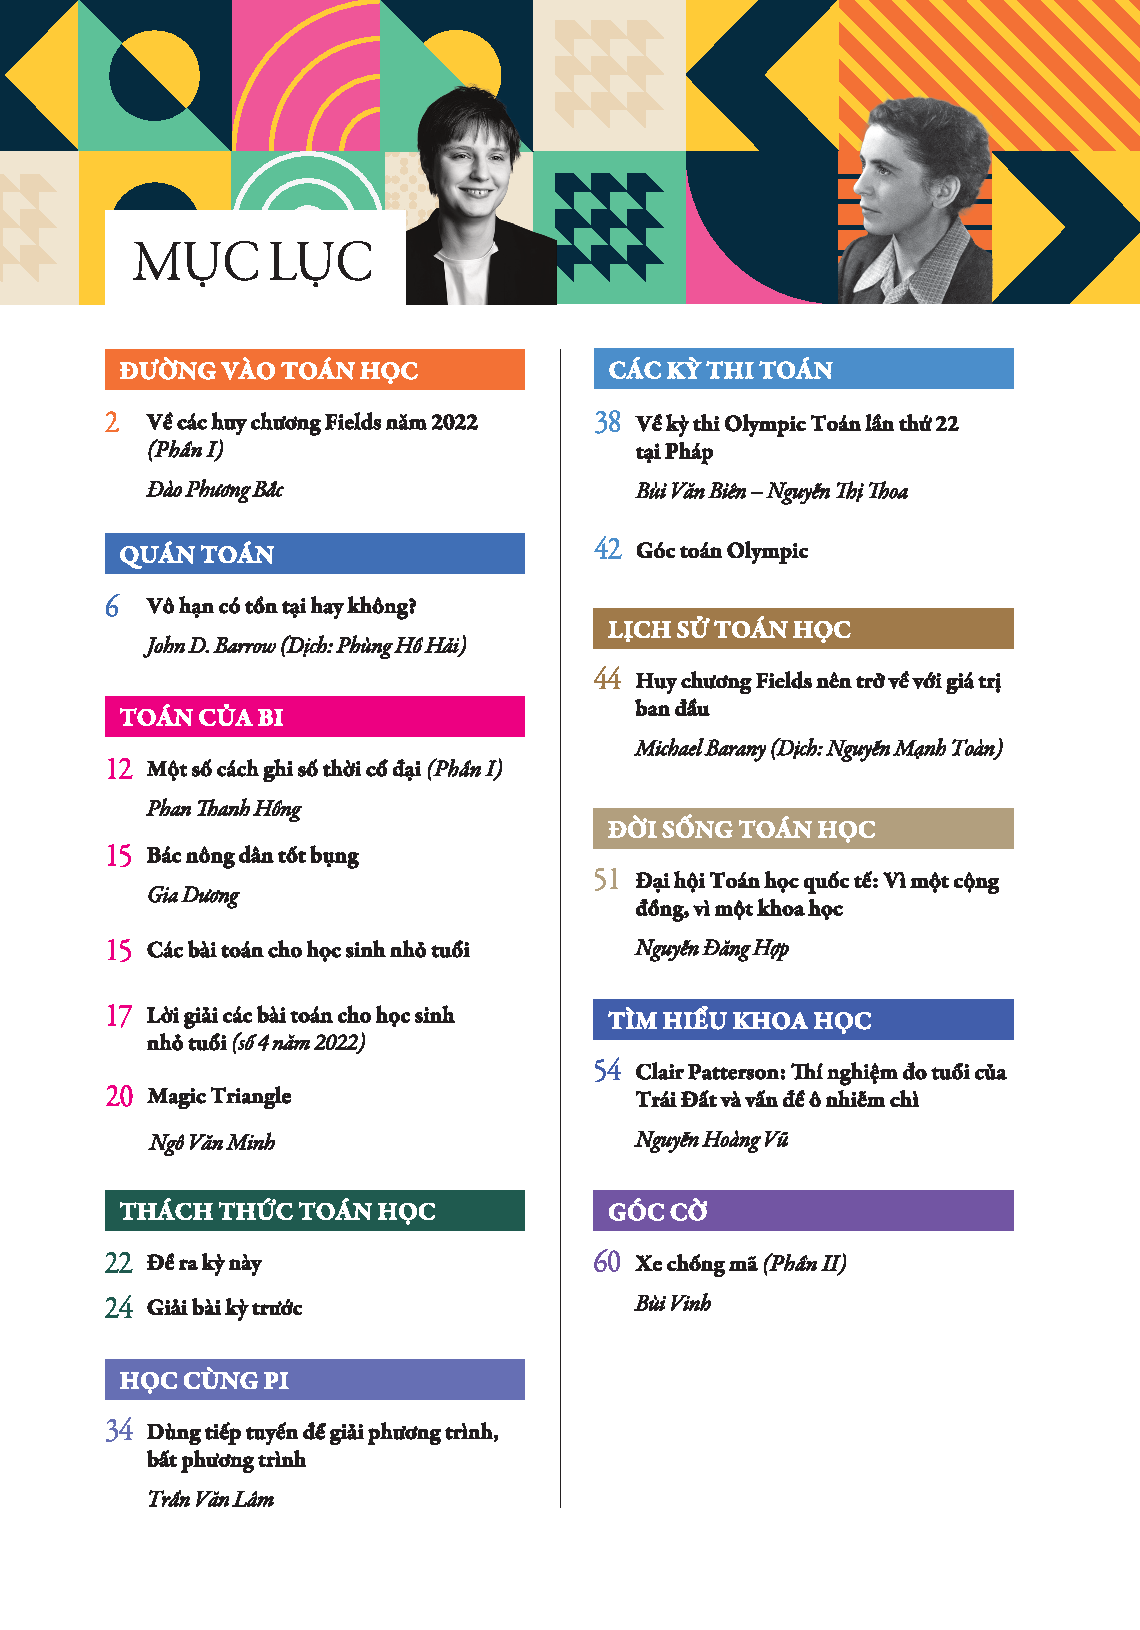
\includegraphics[scale=1]{ML.pdf}}}
%	 \centering
%	 \vspace*{0cm}
%	 \endgroup
%	 \newpage	 
%	 \pagestyle{empty}
%
	\setcounter{page}{2}

	\setcounter{figure}{0}
	\thispagestyle{duongvaotoanhocnone}
\pagestyle{duongvaotoanhoc}
\everymath{\color{duongvaotoanhoc}}
\graphicspath{{../duongvaotoanhoc/pic/}}
\blfootnote{$^1$\color{duongvaotoanhoc}Theo Quanta Magazine.}
\blfootnote{$^2$\color{duongvaotoanhoc}Hà Nội.}
\begingroup
\AddToShipoutPicture*{\put(0,616){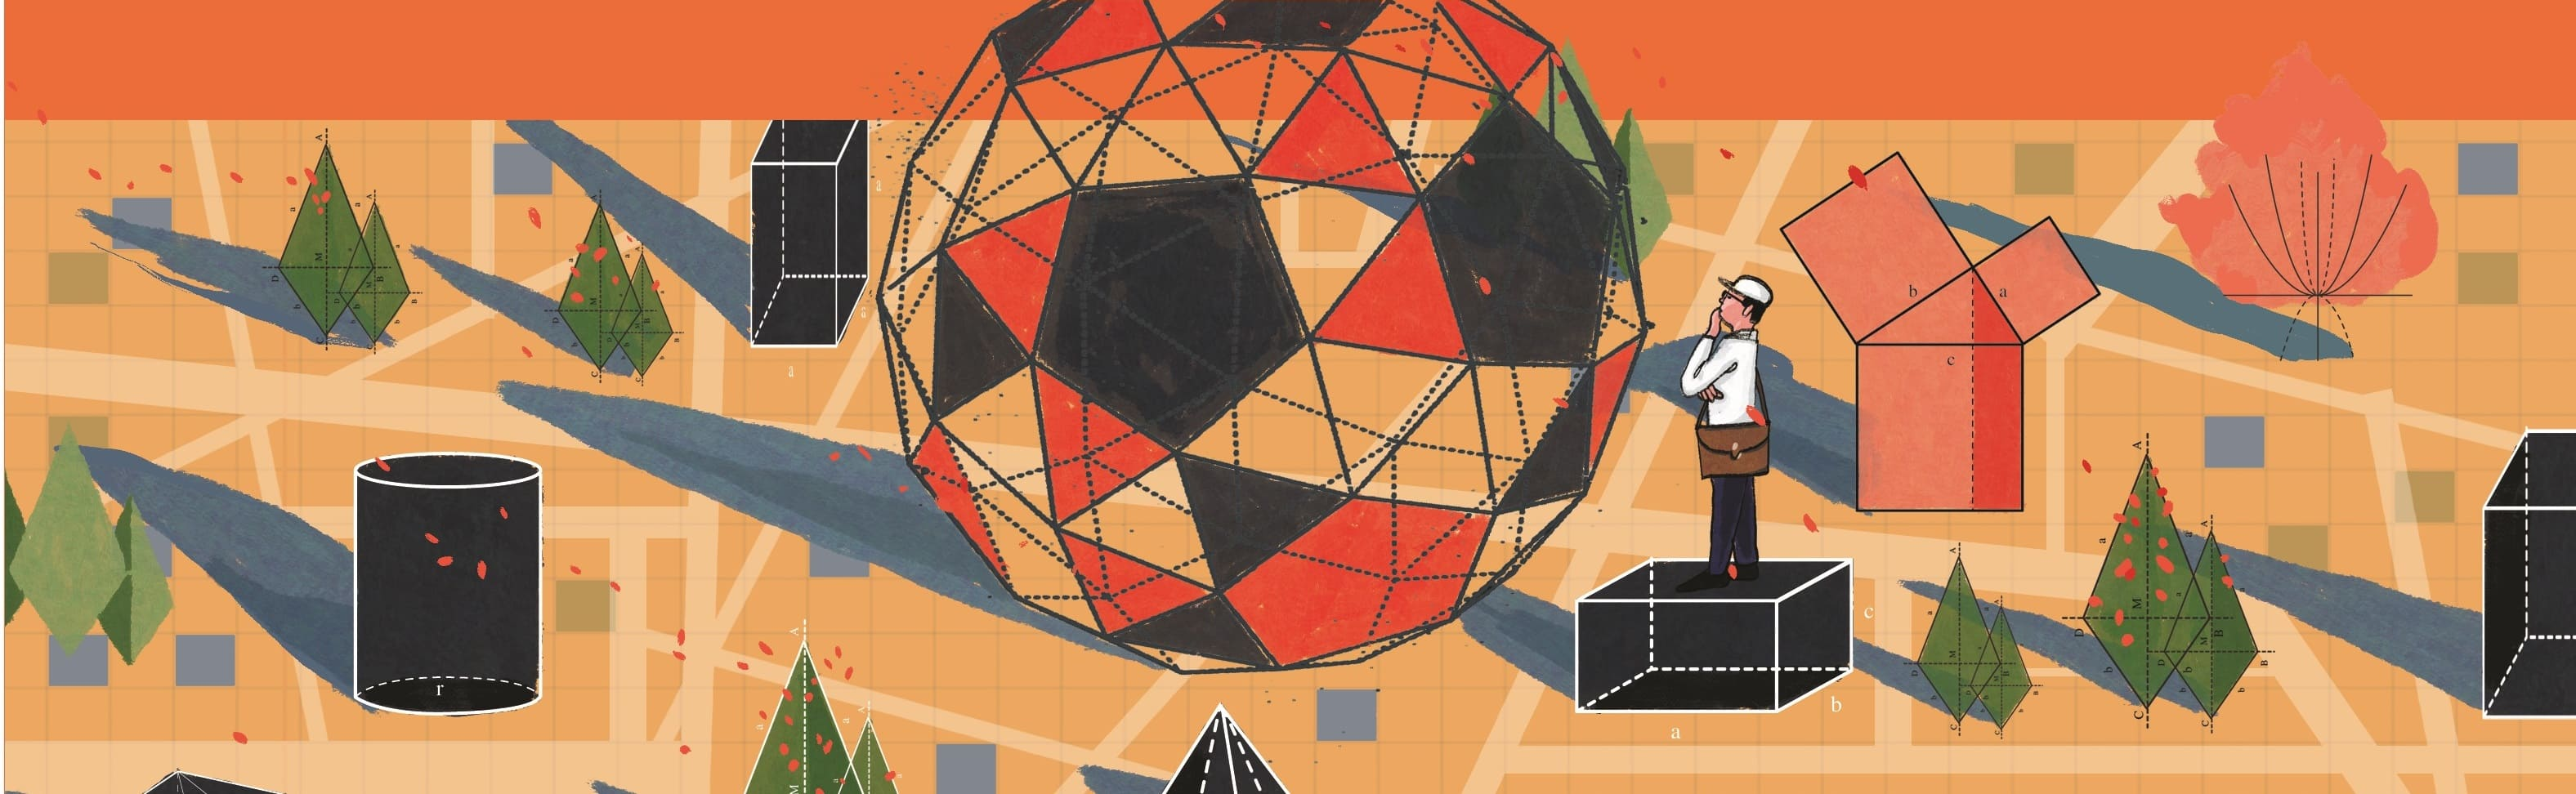
\includegraphics[width=19.3cm]{../bannerduongvao}}}
\AddToShipoutPicture*{\put(136,508){
\includegraphics[scale=1]{../tieude1.pdf}}}
\centering
\endgroup

\vspace*{200pt}

\begin{multicols}{2}	
	\textit{Hai hợp tác gần đây giữa các nhà toán học và công ty DeepMind đã cho thấy tiềm năng của học máy trong việc giúp các nhà nghiên cứu đưa ra các giả thuyết mới trong toán học.}
	\begin{figure}[H]
		\centering
		\vspace*{-5pt}
		\captionsetup{labelformat= empty, justification=centering}
		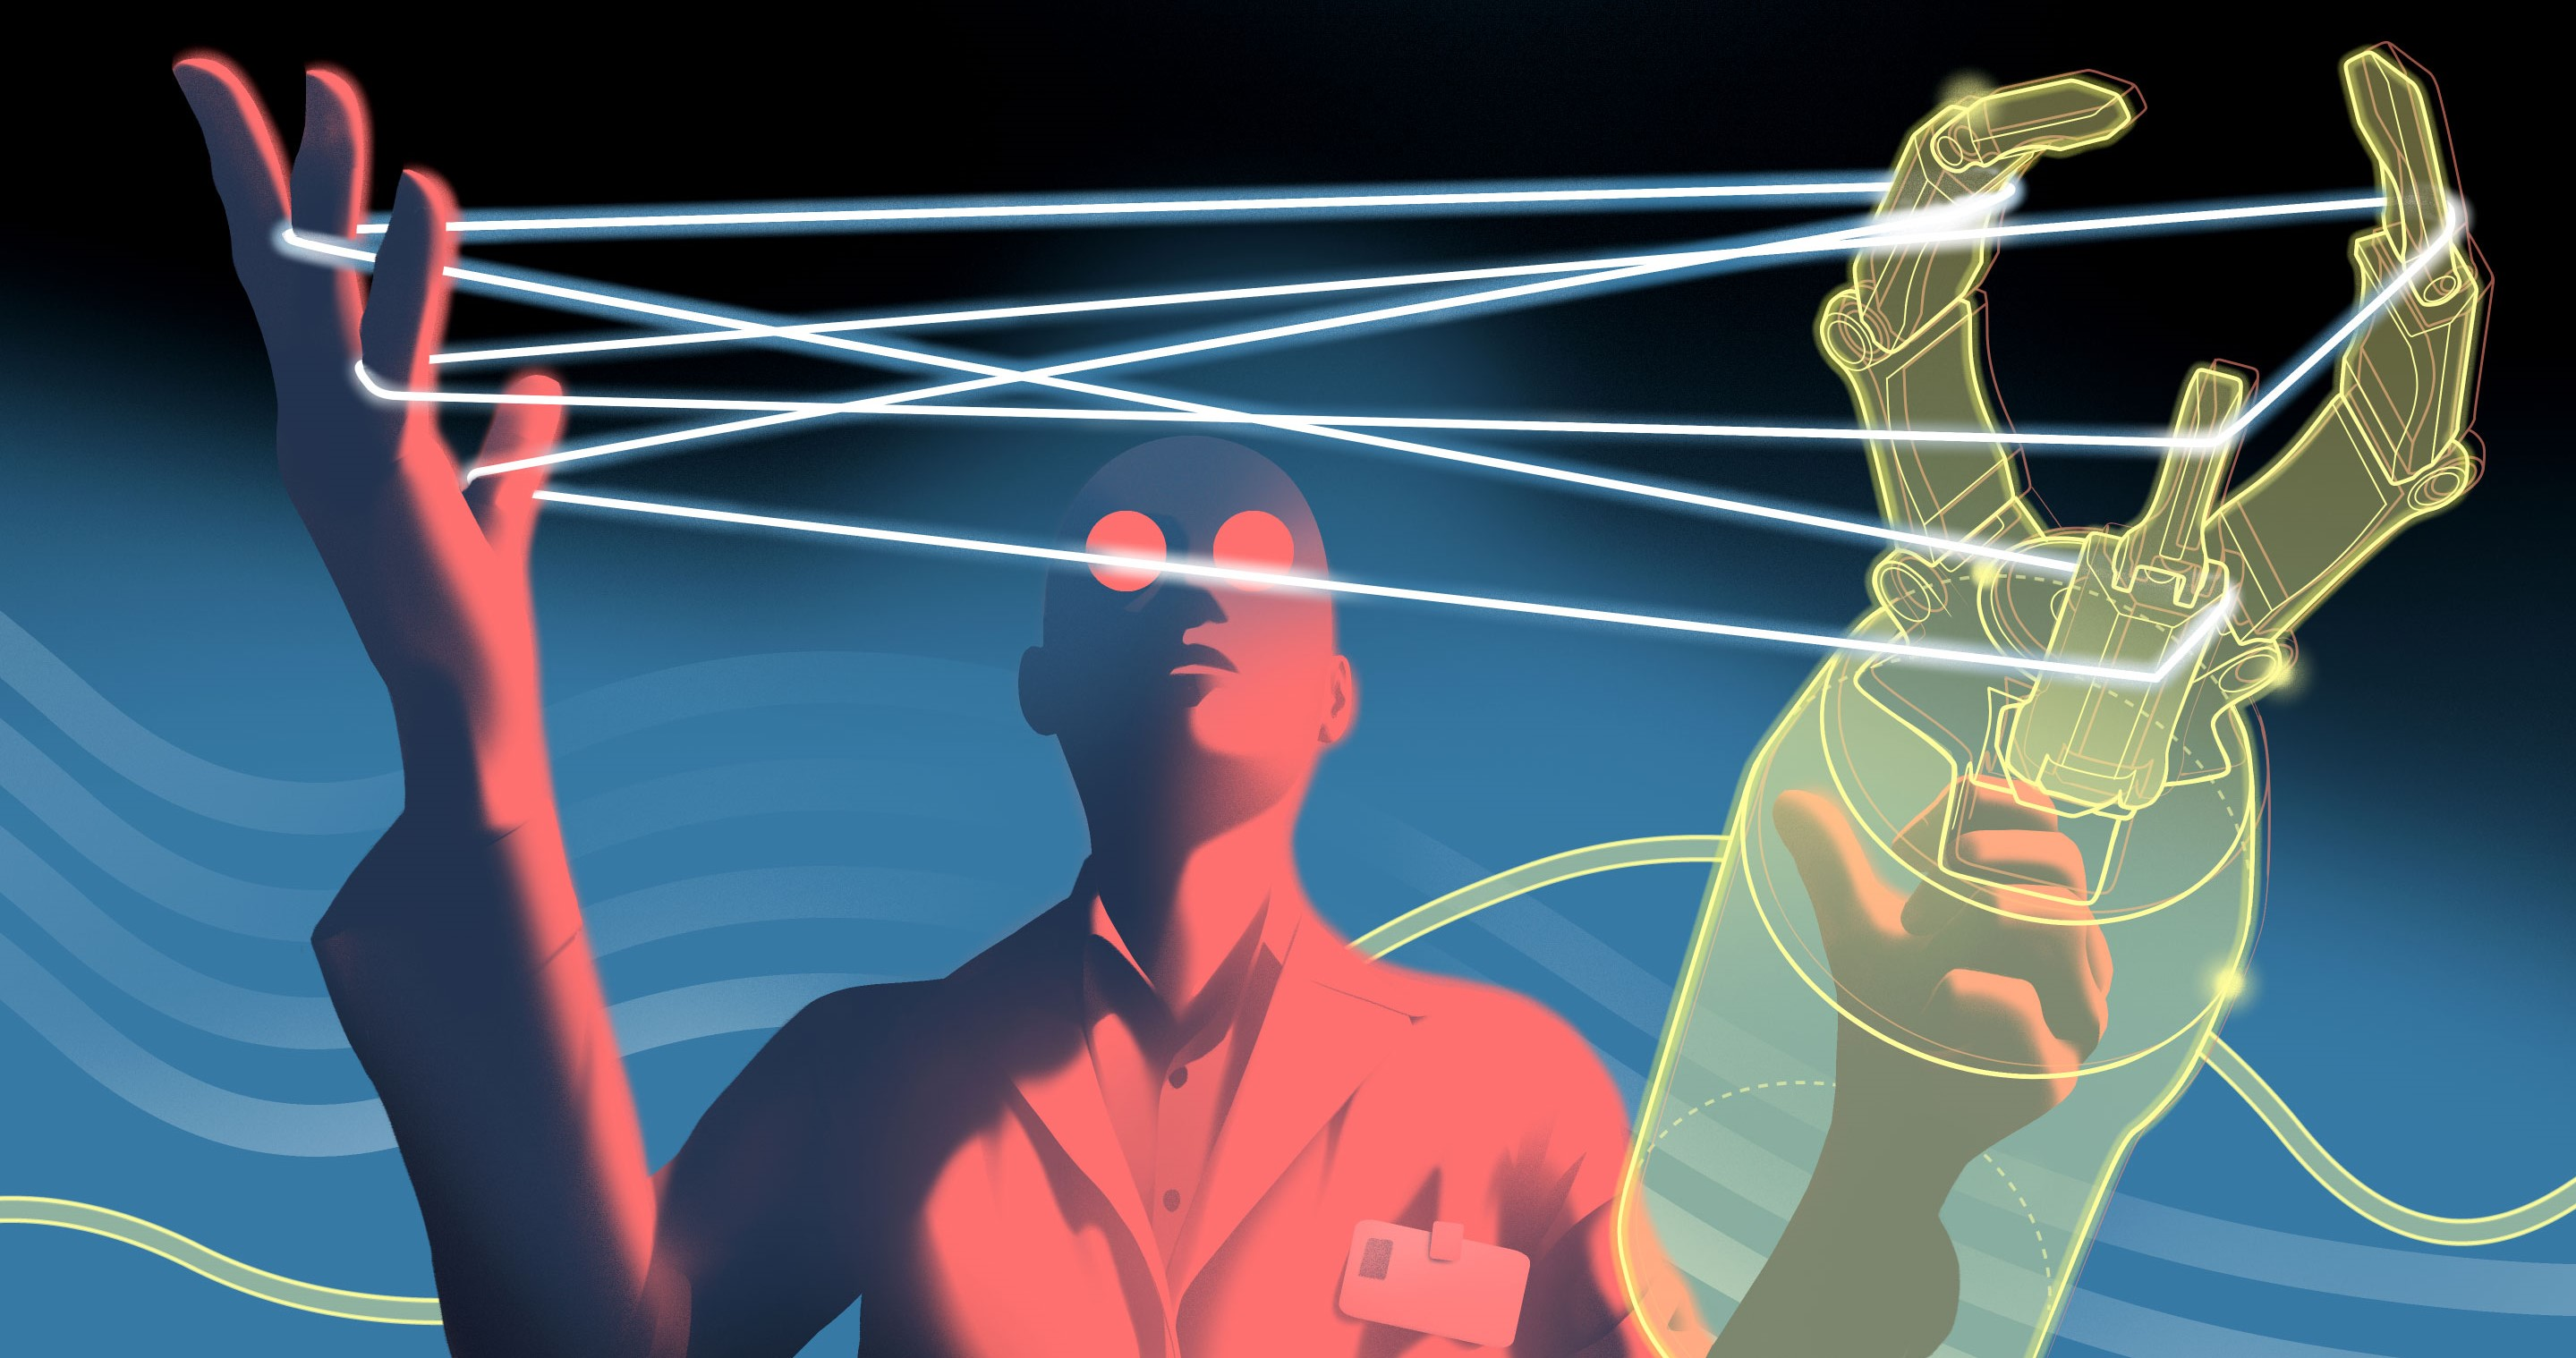
\includegraphics[width=1\linewidth]{1}
		%		\caption{\small\textit{\color{duongvaotoanhoc}Señor Salme, Quanta magazine.}}
		\vspace*{-15pt}
	\end{figure}
	Các nhà toán học thường làm việc cùng nhau khi muốn tìm kiếm những cái nhìn sâu sắc về một vấn đề khó. Đó là một kiểu quy trình cộng tác có vẻ như đòi hỏi hoàn toàn sự trao đổi giữa người và người.
	\vskip 0.05cm
	Nhưng trong hai kết quả mới đây, máy móc đã thay thế một phần vai trò của người cộng tác khoa học. Các bài báo của kiểu hợp tác như vậy được hoàn thành vào cuối tháng $11$ năm $2021$, và được tóm tắt trong một bài báo gần đây trên tạp chí Nature.
	\vskip 0.05cm
	Geordie Williamson, một nhà toán học của Đại học Sydney và là đồng tác giả của một trong những bài báo đó, cho biết: ``Những điều tôi yêu thích ở toán học là các khía cạnh trực giác và sáng tạo của nó. Các mô hình học máy đã hỗ trợ những điều đó theo cách mà trước đây tôi chưa từng cảm nhận được từ máy tính."
	\vskip 0.05cm
	Hai nhóm nhà toán học khác nhau đã làm việc cùng với công ty chuyên phát triển các hệ thống trí tuệ nhân tạo tiên tiến DeepMind, một công ty con của Alphabet (công ty mẹ của Google).
	\vskip 0.05cm
	András Juhász và Marc Lackenby của Đại học Oxford đã dạy các mô hình học máy của DeepMind để tìm kiếm các mẫu lặp trong các đối tượng hình học có tên gọi là \textit{nút}. Các mô hình đã phát hiện ra các kết nối mà Juhász và Lackenby xây dựng ra để liên kết hai lĩnh vực trong lý thuyết nút mà từ lâu các nhà toán học đã phỏng đoán là có liên quan với nhau. Trong một công trình khác, Williamson đã sử dụng các mô hình học máy để tinh chỉnh một giả thuyết cũ kết nối giữa đồ thị và đa thức.
	\vskip 0.05cm
	Trong nhiều năm, máy tính đã hỗ trợ nghiên cứu toán học như một công cụ trợ giúp chứng minh nhằm đảm bảo tính đúng đắn trong các bước suy luận logic của một chứng minh toán học, hoặc như một công cụ mạnh có thể xử lý một lượng lớn các dữ liệu để tìm ra các phản ví dụ cho các giả thuyết.
	\vskip 0.05cm
	Các công trình mới kể trên đại diện cho một hình thức hợp tác khác giữa con người và máy móc. Nó chỉ ra rằng bằng cách kết hợp một cách có chọn lọc học máy vào giai đoạn phát triển của nghiên cứu, các nhà toán học có thể phát hiện ra các manh mối mà có thể khó tìm thấy chúng nếu không có sự trợ giúp của máy móc.
	\vskip 0.05cm
	Radmila Sazdanovic của Đại học Bang North Carolina cho biết: ``Điều tuyệt vời nhất về các công trình này -- và nó thực sự là một bước đột phá lớn -- là tất cả các mảnh ghép khớp lại với nhau và những người này đã làm việc như một nhóm. Đó thực sự là một hợp tác liên ngành."
	\vskip 0.05cm
	Tuy nhiên, một số nhà quan sát coi những hợp tác này không phải là một cuộc cách mạng trong cách thức tiến hành nghiên cứu toán học. Trong khi máy tính hướng các nhà toán học tới một loạt các mối quan hệ có thể có thì bản thân các nhà toán học cần xác định xem những mối quan hệ nào là đáng khám phá.
	\vskip 0.05cm
	Ernest Davis, một nhà khoa học máy tính của Đại học New York, viết trong email: ``Tất cả những công việc khó khăn đều được thực hiện bởi con người -- các nhà toán học."
	\vskip 0.05cm
	\textbf{\color{duongvaotoanhoc}Các mẫu lặp trong dữ liệu}
	\vskip 0.05cm
	Học máy dự đoán kết quả đầu ra dựa vào dữ liệu đầu vào: nếu cung cấp cho nó một dữ liệu điển hình về sức khỏe thì nó sẽ đưa ra một chẩn đoán lâm sàng; nếu đưa cho nó hình ảnh của một con vật thì nó sẽ cho biết tên của loài đó.
	\vskip 0.05cm
	Điều này thường được thực hiện thông qua tiếp cận học máy có tên là học có giám sát, trong đó các nhà nghiên cứu chủ yếu dạy máy tính đưa ra dự đoán bằng cách cung cấp cho nó nhiều ví dụ.
	\vskip 0.05cm
	Chẳng hạn, hãy tưởng tượng bạn muốn dạy một mô hình học máy xác định xem một bức ảnh chụp một con mèo hay là một con chó. Đầu tiên, các nhà nghiên cứu cung cấp cho mô hình học máy nhiều ví dụ về mỗi loài. Dựa trên các dữ liệu huấn luyện đó, máy tính xây dựng một hàm toán học cực kỳ phức tạp, mà về bản chất là một cỗ máy đưa ra các dự đoán. Sau đó, một khi chức năng dự đoán đã được thiết lập, các nhà nghiên cứu đưa ra một bức ảnh mới cho mô hình và nó sẽ trả lời đó là mèo hay chó với xác suất tương ứng.
	\begin{figure}[H]
		\centering
		\vspace*{-5pt}
		\captionsetup{labelformat= empty, justification=centering}
		
\includegraphics[width=1\linewidth]{2}
		\caption{\small\textit{\color{duongvaotoanhoc}Geordie Williamson của Đại học Sydney đã giúp DeepMind xác định các vấn đề toán học phù hợp với học máy.}}
		\vspace*{-10pt}
	\end{figure}
	Để khiến việc học có giám sát trở thành một công cụ nghiên cứu hữu ích, các nhà toán học phải tìm ra những câu hỏi phù hợp để DeepMind giải quyết. Họ cần các bài toán liên quan đến các đối tượng toán học mà ở đó có sẵn nhiều dữ liệu huấn luyện -- một tiêu chí mà nhiều vấn đề toán học không đáp ứng được.
	\vskip 0.05cm
	Họ cũng cần tìm cách tận dụng khả năng mạnh mẽ của DeepMind trong việc phát hiện các mối liên hệ tiềm ẩn, đồng thời khắc phục những hạn chế đáng kể của nó với vai trò là cộng tác viên khoa học. Thông thường, mô hình học máy hoạt động như một hộp đen, tạo ra kết quả đầu ra từ các dữ liệu đầu vào theo các quy tắc mà con người không thể giải mã được.
	\vskip 0.05cm
	Alex Davies, một nhà nghiên cứu tại DeepMind, cho biết: ``[Máy tính] có thể nhìn thấy những điều bất thường, nhưng cũng phải vật lộn để giải thích một cách hiệu quả."
	\vskip 0.05cm
	Các nhà toán học không tìm đến DeepMind chỉ để có các câu trả lời đúng. Để thực sự có những tiến bộ khoa học, họ cần biết lý do vì sao lại có các mối liên hệ – bước mà máy tính không thể làm được.
	\vskip 0.05cm
	\textbf{\color{duongvaotoanhoc}Kết nối các bất biến}
	\vskip 0.05cm
	Năm $2018$, Williamson và Demis Hassabis, giám đốc điều hành và đồng sáng lập của DeepMind, cùng được bầu làm thành viên của Hội Khoa học Hoàng gia Anh (Royal Society), một tổ chức gồm các nhà khoa học xuất sắc của Anh. Trong  giờ nghỉ giải lao tại buổi lễ kết nạp, họ nhận thấy có những mối quan tâm chung.
	\vskip 0.05cm
	Williamson nói: ``Tôi đã suy nghĩ một chút ít về cách học máy có thể giúp ích cho toán học và anh ấy đã suy nghĩ rất nhiều về điều đó. Kiểu như chúng tôi nảy ra những ý tưởng từ nhau."
	\vskip 0.05cm
	Họ quyết định rằng một chuyên ngành toán học được gọi là lý thuyết nút sẽ là nền tảng thử nghiệm lý tưởng cho sự hợp tác giữa con người và máy tính. Nó liên quan đến các đối tượng toán học có tên gọi là nút, mà bạn có thể coi như những vòng dây chằng chịt. Lý thuyết nút phù hợp với các yêu cầu đối với học máy vì nó có dữ liệu phong phú -- có hàng triệu nút tương đối đơn giản -- và vì nhiều thuộc tính của nút thắt có thể được tính toán dễ dàng bằng phần mềm hiện có.
	\vskip 0.05cm
	Williamson đề nghị DeepMind liên hệ với Lackenby, một nhà lý thuyết nút có tiếng, để tìm ra một vấn đề toán học cụ thể để giải quyết.
	\vskip 0.05cm	
	Juhász và Lackenby hiểu rõ điểm mạnh và điểm yếu của học máy. Với những thứ đó, họ hy vọng sẽ sử dụng nó để tìm ra những mối liên hệ mới giữa các loại bất biến khác nhau, những thuộc tính được sử dụng để phân biệt các nút với nhau.
	\vskip 0.05cm
	Hai nút được coi là khác nhau khi không thể tháo gỡ chúng (mà không cắt chúng) để chúng trông giống nhau. Bất biến là các thuộc tính bản chất của nút, không thay đổi trong quá trình tháo gỡ (do đó có tên là ``bất biến"). Vì vậy, nếu hai nút có một bất biến nhận các giá trị khác nhau, thì không thể thao tác để chúng trở nên giống nhau.
	\begin{figure}[H]
		\centering
		\vspace*{-5pt}
		\captionsetup{labelformat= empty, justification=centering}
		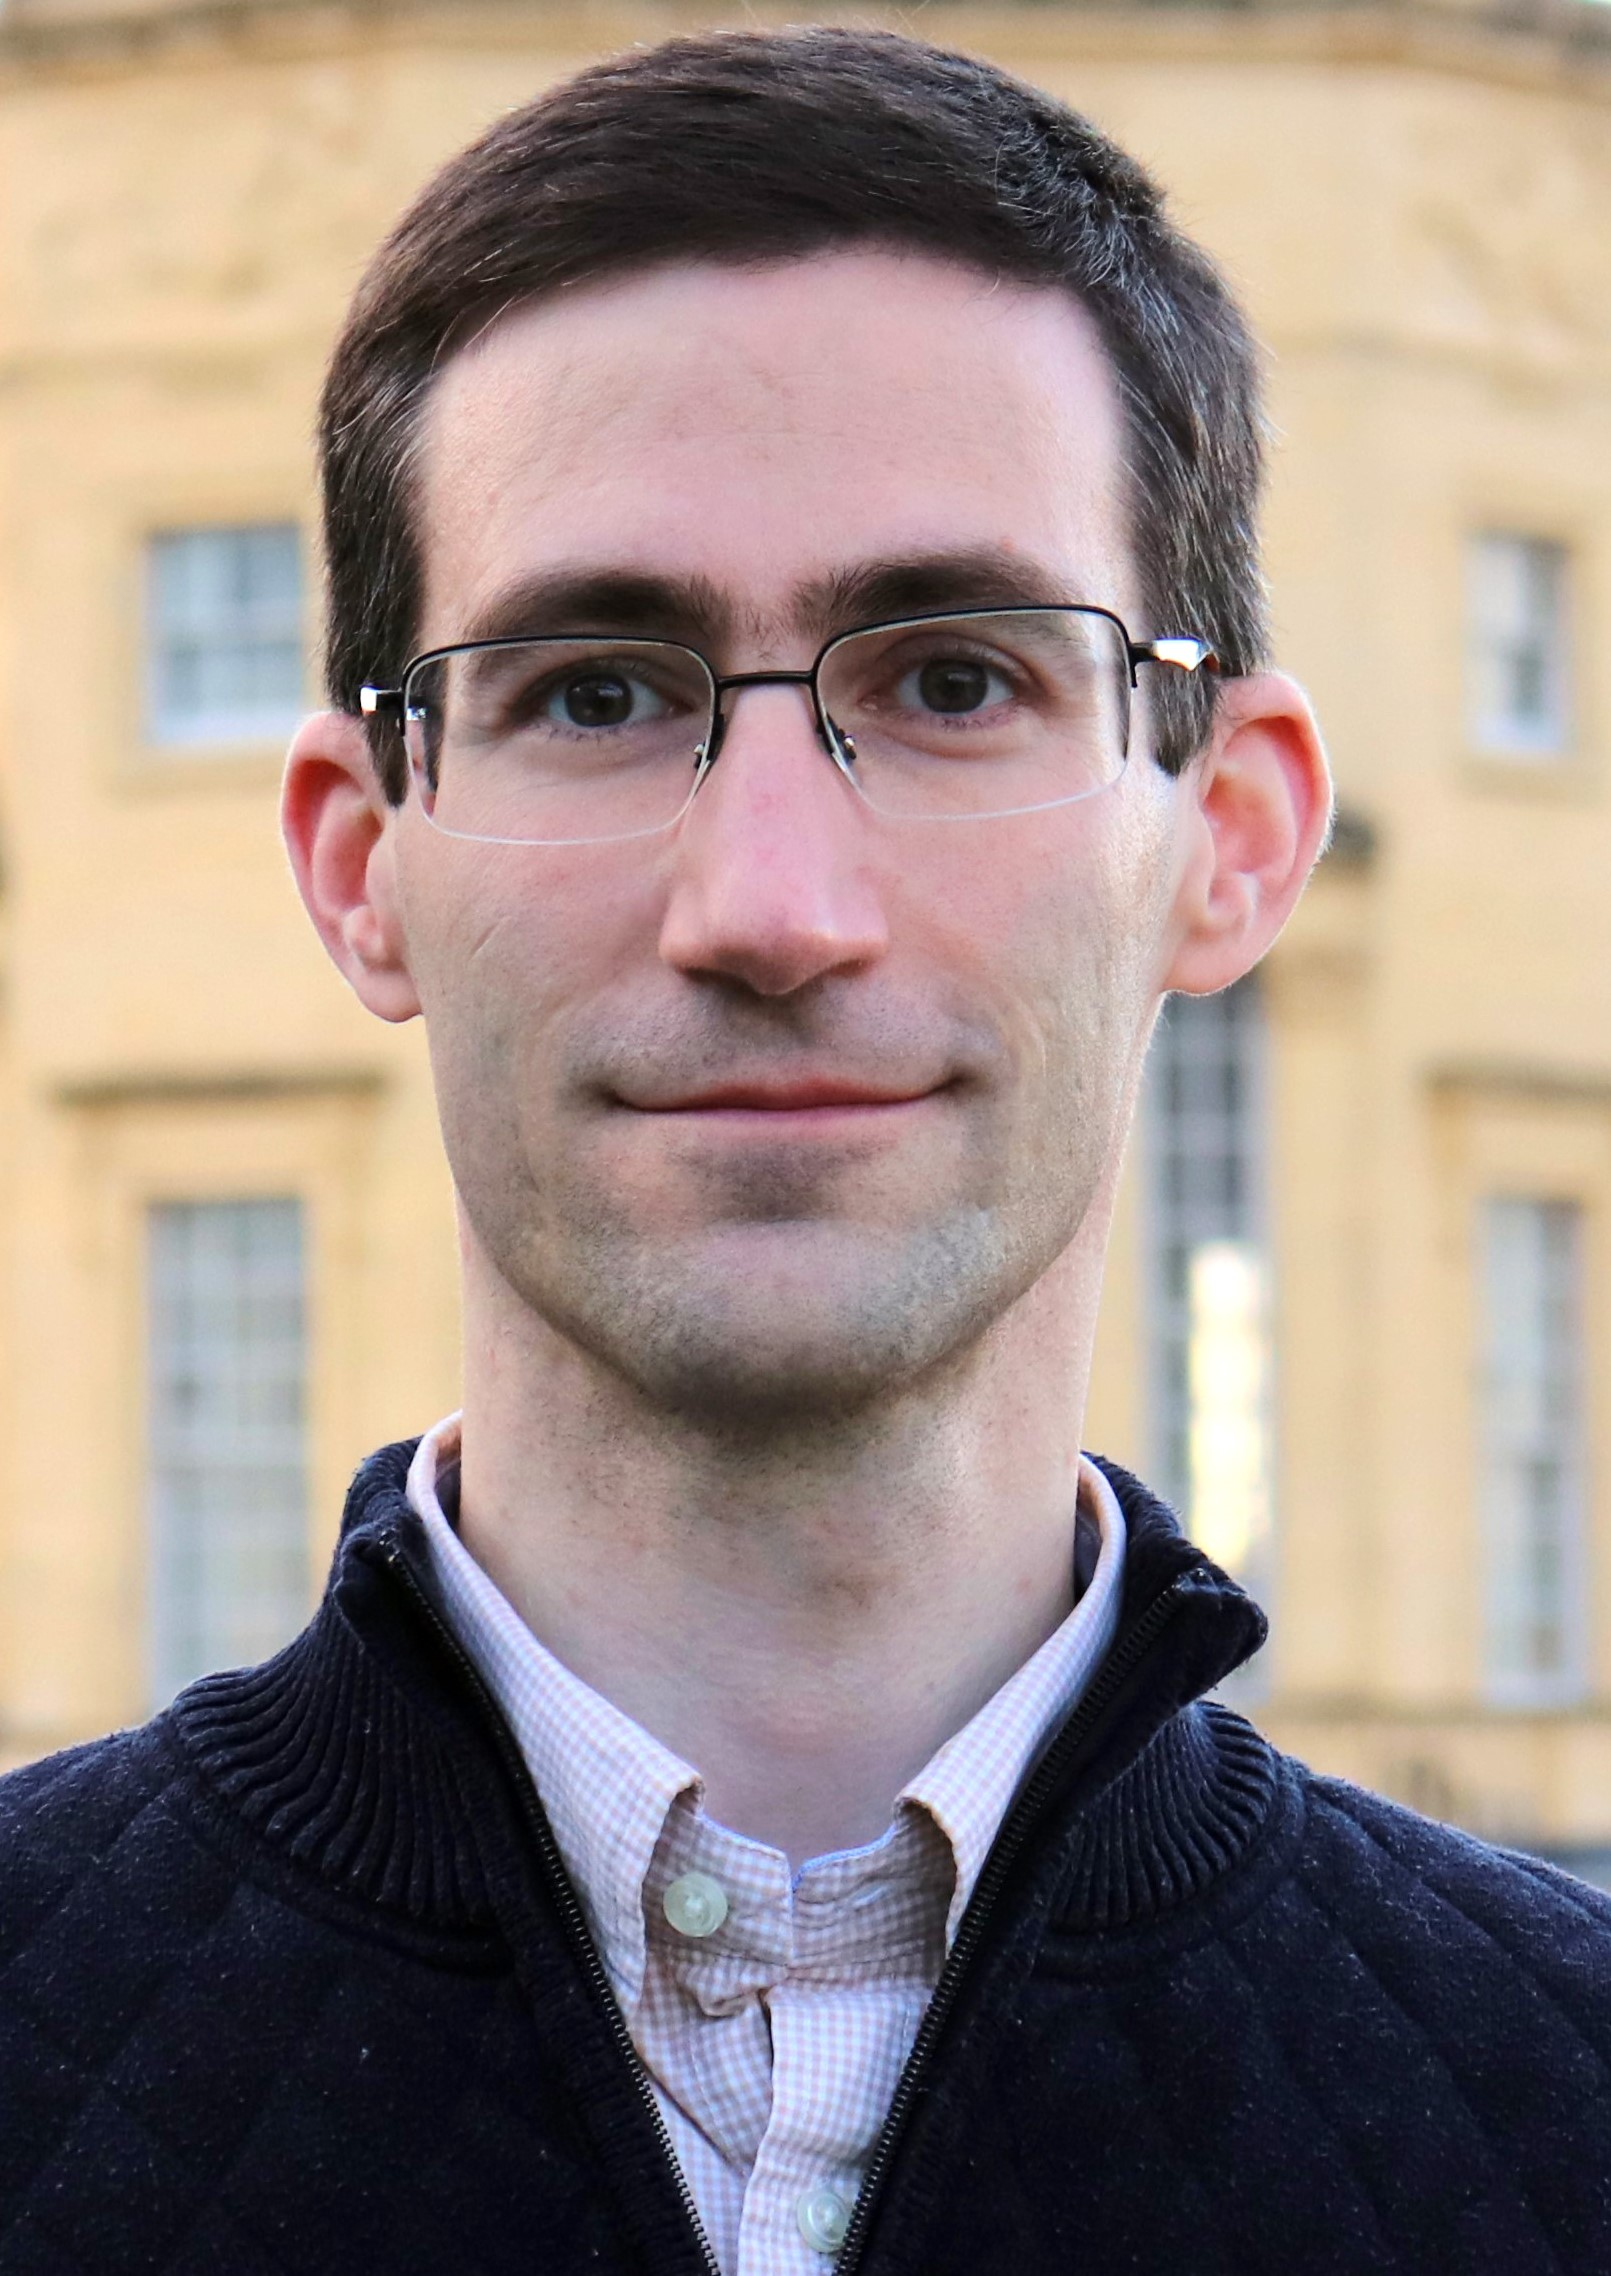
\includegraphics[height=0.425\linewidth]{3}
		
\includegraphics[height=0.425\linewidth]{4}
		\caption{\small\textit{\color{duongvaotoanhoc}András Juhász và Marc Lackenby của Đại học Oxford đã chọn lọc  một tập hợp các manh mối được tạo ra nhờ học máy để xác định một công thức phiên dịch giữa các bất biến nút thắt khác~nhau.}}
		\vspace*{-10pt}
	\end{figure}
	Có nhiều loại bất biến nút khác nhau, được đặc trưng bởi cách mà chúng mô tả các nút. Một số trong chúng mang tính hình học nhiều hơn, một số khác mang tính đại số và một số thì có tính tổ hợp. Tuy nhiên, các nhà toán học chỉ có thể thiết lập được rất ít mối quan hệ giữa các bất biến thuộc các loại khác nhau. Họ thường không biết liệu các bất biến khác nhau có thực chất đo lường cùng một đặc điểm của nút từ các góc nhìn khác nhau hay không.
	\vskip 0.05cm
	\textbf{\color{duongvaotoanhoc}Xác minh chữ ký}
	\vskip 0.05cm
	Để theo đuổi câu hỏi của Juhász và Lackenby, các nhà nghiên cứu tại DeepMind đã phát triển một bộ dữ liệu với hơn 2 triệu nút. Đối với mỗi nút, họ tính toán các bất biến khác nhau. Sau đó, họ sử dụng học máy để tìm kiếm các mẫu lặp gắn kết các bất biến với nhau. Máy tính phát hiện được nhiều mẫu, nhưng hầu hết trong số đó không quá thú vị đối với các nhà toán học.
	\vskip 0.05cm
	``Chúng tôi thấy khá nhiều mẫu lặp đã được biết đến hoặc đã được chỉ ra là không đúng," Lackenby nói. ``Là những nhà toán học, chúng tôi đã loại bỏ khá nhiều thứ mà máy tính gửi cho chúng tôi."
	\vskip 0.05cm
	Không giống như Juhász và Lackenby, hệ thống học máy không hiểu được lý thuyết toán học đằng sau. Dữ liệu đầu vào được tính toán từ các bất biến nút, nhưng máy tính chỉ nhìn thấy danh sách các con số.
	\vskip 0.05cm
	Davis cho biết: ``Về phía hệ thống học máy, các con số đó cũng giống như doanh số bán hàng của nhiều món ăn khác nhau tại cửa hàng McDonald mà thôi."
	\vskip 0.05cm
	Cuối cùng, hai nhà toán học quyết định tìm cách dạy máy tính xuất ra một bất biến đại số quan trọng được gọi là "chữ ký" của một nút chỉ dựa trên thông tin về các bất biến hình học của nút.
	\vskip 0.05cm
	Sau khi Juhász và Lackenby xác định được vấn đề, các nhà nghiên cứu tại DeepMind bắt đầu xây dựng thuật toán học máy cụ thể. Họ đã huấn luyện máy tính lấy $30$ bất biến hình học của một nút làm đầu vào và xuất ra chữ ký của nút. Thuật toán hoạt động tốt và sau một vài tuần làm việc, DeepMind có thể dự đoán chính xác chữ ký của hầu hết các nút.
	\vskip 0.05cm
	Tiếp theo, các nhà nghiên cứu cần tìm hiểu xem mô hình học máy đã đưa ra những dự đoán này như thế nào. Để làm điều đó, nhóm nghiên cứu tại DeepMind quay sang một kỹ thuật được gọi là phân tích độ quan trọng, được sử dụng để xác định xem đầu vào nào có tác động lớn nhất trong việc tạo ra kết quả đầu ra. Họ thay đổi một chút giá trị của từng đầu vào, mỗi lần chỉ thay đổi một giá trị, và kiểm tra xem thay đổi nào có tác động mạnh nhất đến kết quả đầu ra.
	\vskip 0.05cm
	Nếu một thuật toán được thiết kế để dự đoán liệu bức ảnh có phải là của một con mèo hay không, khi thực hiện phân tích độ quan trọng, các nhà nghiên cứu sẽ làm mờ một số mảnh nhỏ của bức ảnh và sau đó kiểm tra xem máy tính có còn nhận ra con mèo hay không. Chẳng hạn, họ có thể nhận thấy rằng các điểm ảnh ở góc của bức ảnh ít quan trọng hơn so với các điểm ảnh tạo nên tai mèo.
	\vskip 0.05cm
	Khi các nhà nghiên cứu áp dụng kỹ thuật phân tích độ quan trọng vào dữ liệu về nút, họ quan sát được rằng $3$ trong số $30$ bất biến hình học dường như đặc biệt quan trọng đối với cách mà mô hình học máy đưa ra dự đoán. Cả ba bất biến này đều đo lường các đặc điểm về mũi của nút, một ống rỗng bao quanh nút, giống như lớp cao su bọc xung quanh một sợi cáp.
	\vskip 0.05cm
	Dựa trên thông tin này, Juhász và Lackenby xây dựng một công thức liên hệ chữ ký của một nút với ba bất biến hình học đó. Công thức cũng sử dụng một bất biến phổ biến khác, là thể tích của một hình cầu mà nút được khoét ra từ đó. Khi họ kiểm tra công thức trên các nút cụ thể, nó có vẻ như là đúng, nhưng điều đó không đủ để khẳng định một định lý toán học mới. Các nhà toán học tìm kiếm một phát biểu phù hợp mà họ có thể chứng minh là đúng -- và điều đó còn khó hơn.
	\vskip 0.05cm
	``Mọi chuyện diễn ra không suôn sẻ lắm," Lackenby kể.
	\vskip 0.05cm
	Trực giác của Juhász và Lackenby, được hình thành qua nhiều năm nghiên cứu các vấn đề tương tự, cho họ biết rằng công thức vẫn còn thiếu một thứ gì đó. Họ nhận ra rằng cần phải đưa ra một bất biến hình học khác, gọi là bán kính đơn ánh, nôm na đo lường chiều dài của một số đường cong liên quan đến nút. Đó là một bước sử dụng thứ trực giác được rèn giũa của các nhà toán học, nhưng được kích hoạt nhờ những hiểu biết cụ thể mà họ thu thập được từ những mối liên kết thô mà mô hình học máy của DeepMind xác định được.
	\vskip 0.05cm
	``Thật tốt là các mô hình học máy có những điểm mạnh và điểm yếu hoàn toàn ngược với con người," Adam Zsolt Wagner, Đại học Tel Aviv, nói.
	\vskip 0.05cm
	Việc điều chỉnh đã thành công. Bằng cách kết hợp thông tin về bán kính đơn ánh với ba bất biến hình học được DeepMind xác định, Juhász và Lackenby tạo ra được một công thức chặt chẽ để tính chữ ký của một nút. Kết quả cuối cùng có tinh thần của một sự hợp tác thực sự.
	\vskip 0.05cm
	``Đó quả thực là một quá trình nhiều bước, có sự tham gia của cả các chuyên gia học máy của DeepMind và chúng tôi", Lackenby kể~lại.
	\vskip 0.05cm
	\textbf{\color{duongvaotoanhoc}Chuyển đổi đồ thị thành đa thức}
	\vskip 0.05cm
	Dựa trên đà phát triển của dự án về lý thuyết nút, vào đầu năm $2020$, DeepMind quay sang  Williamson để xem liệu anh có muốn thử nghiệm một quy trình tương tự trong lĩnh vực của mình, lý thuyết biểu diễn, hay không. Lý thuyết biểu diễn là một nhánh của toán học nghiên cứu các cách kết hợp các yếu tố cơ bản của toán học như các đối xứng để tạo ra các đối tượng phức tạp hơn.
	\vskip 0.05cm
	Trong chuyên ngành này, các đa thức Kazhdan--Lusztig là các đối tượng đặc biệt quan trọng. Chúng được xây dựng dựa trên các cách sắp xếp lại các vật nào đó -- chẳng hạn như cách hoán đổi thứ tự của hai vật trong một danh sách các vật cho trước -- được gọi là hoán vị. Mỗi đa thức Kazhdan--Lusztig được xây dựng từ một cặp hoán vị và mã hóa thông tin về mối quan hệ của chúng. Chúng rất bí ẩn và có các hệ số thường rất khó tính toán.
	\vskip 0.05cm
	Do đó, các nhà toán học cố gắng hiểu đa thức Kazhdan--Lusztig thông qua các đối tượng dễ làm việc hơn, gọi là đồ thị Bruhat. Mỗi đỉnh của đồ thị Bruhat biểu diễn một hoán vị của cùng một số các vật cụ thể. Các cạnh nối các đỉnh tương ứng với các hoán vị chỉ khác nhau một phép hoán đổi thứ tự của hai vật trong~đó.
	\vskip 0.05cm
	Vào những năm $1980$, George Lusztig và Matthew Dyer, một cách độc lập với nhau, đã dự đoán rằng phải có mối quan hệ giữa đồ thị Bruhat và đa thức Kazhdan--Lusztig. Mối quan hệ như vậy sẽ hữu ích vì đa thức là đối tượng nền tảng hơn, trong khi đồ thị lại đơn giản hơn trong các tính toán.
	\vskip 0.05cm
	Và, cũng giống như bài toán dự đoán một bất biến nút bằng cách sử dụng một bất biến nút khác, bài toán này rất phù hợp với năng lực của DeepMind. Ban đầu, nhóm nghiên cứu của DeepMind huấn luyện mô hình học máy trên gần $20{.}000$ đồ thị ghép đôi Bruhat và đa thức Kazhdan--Lusztig.
	\begin{figure}[H]
		\centering
		\vspace*{-10pt}
		\captionsetup{labelformat= empty, justification=centering}
		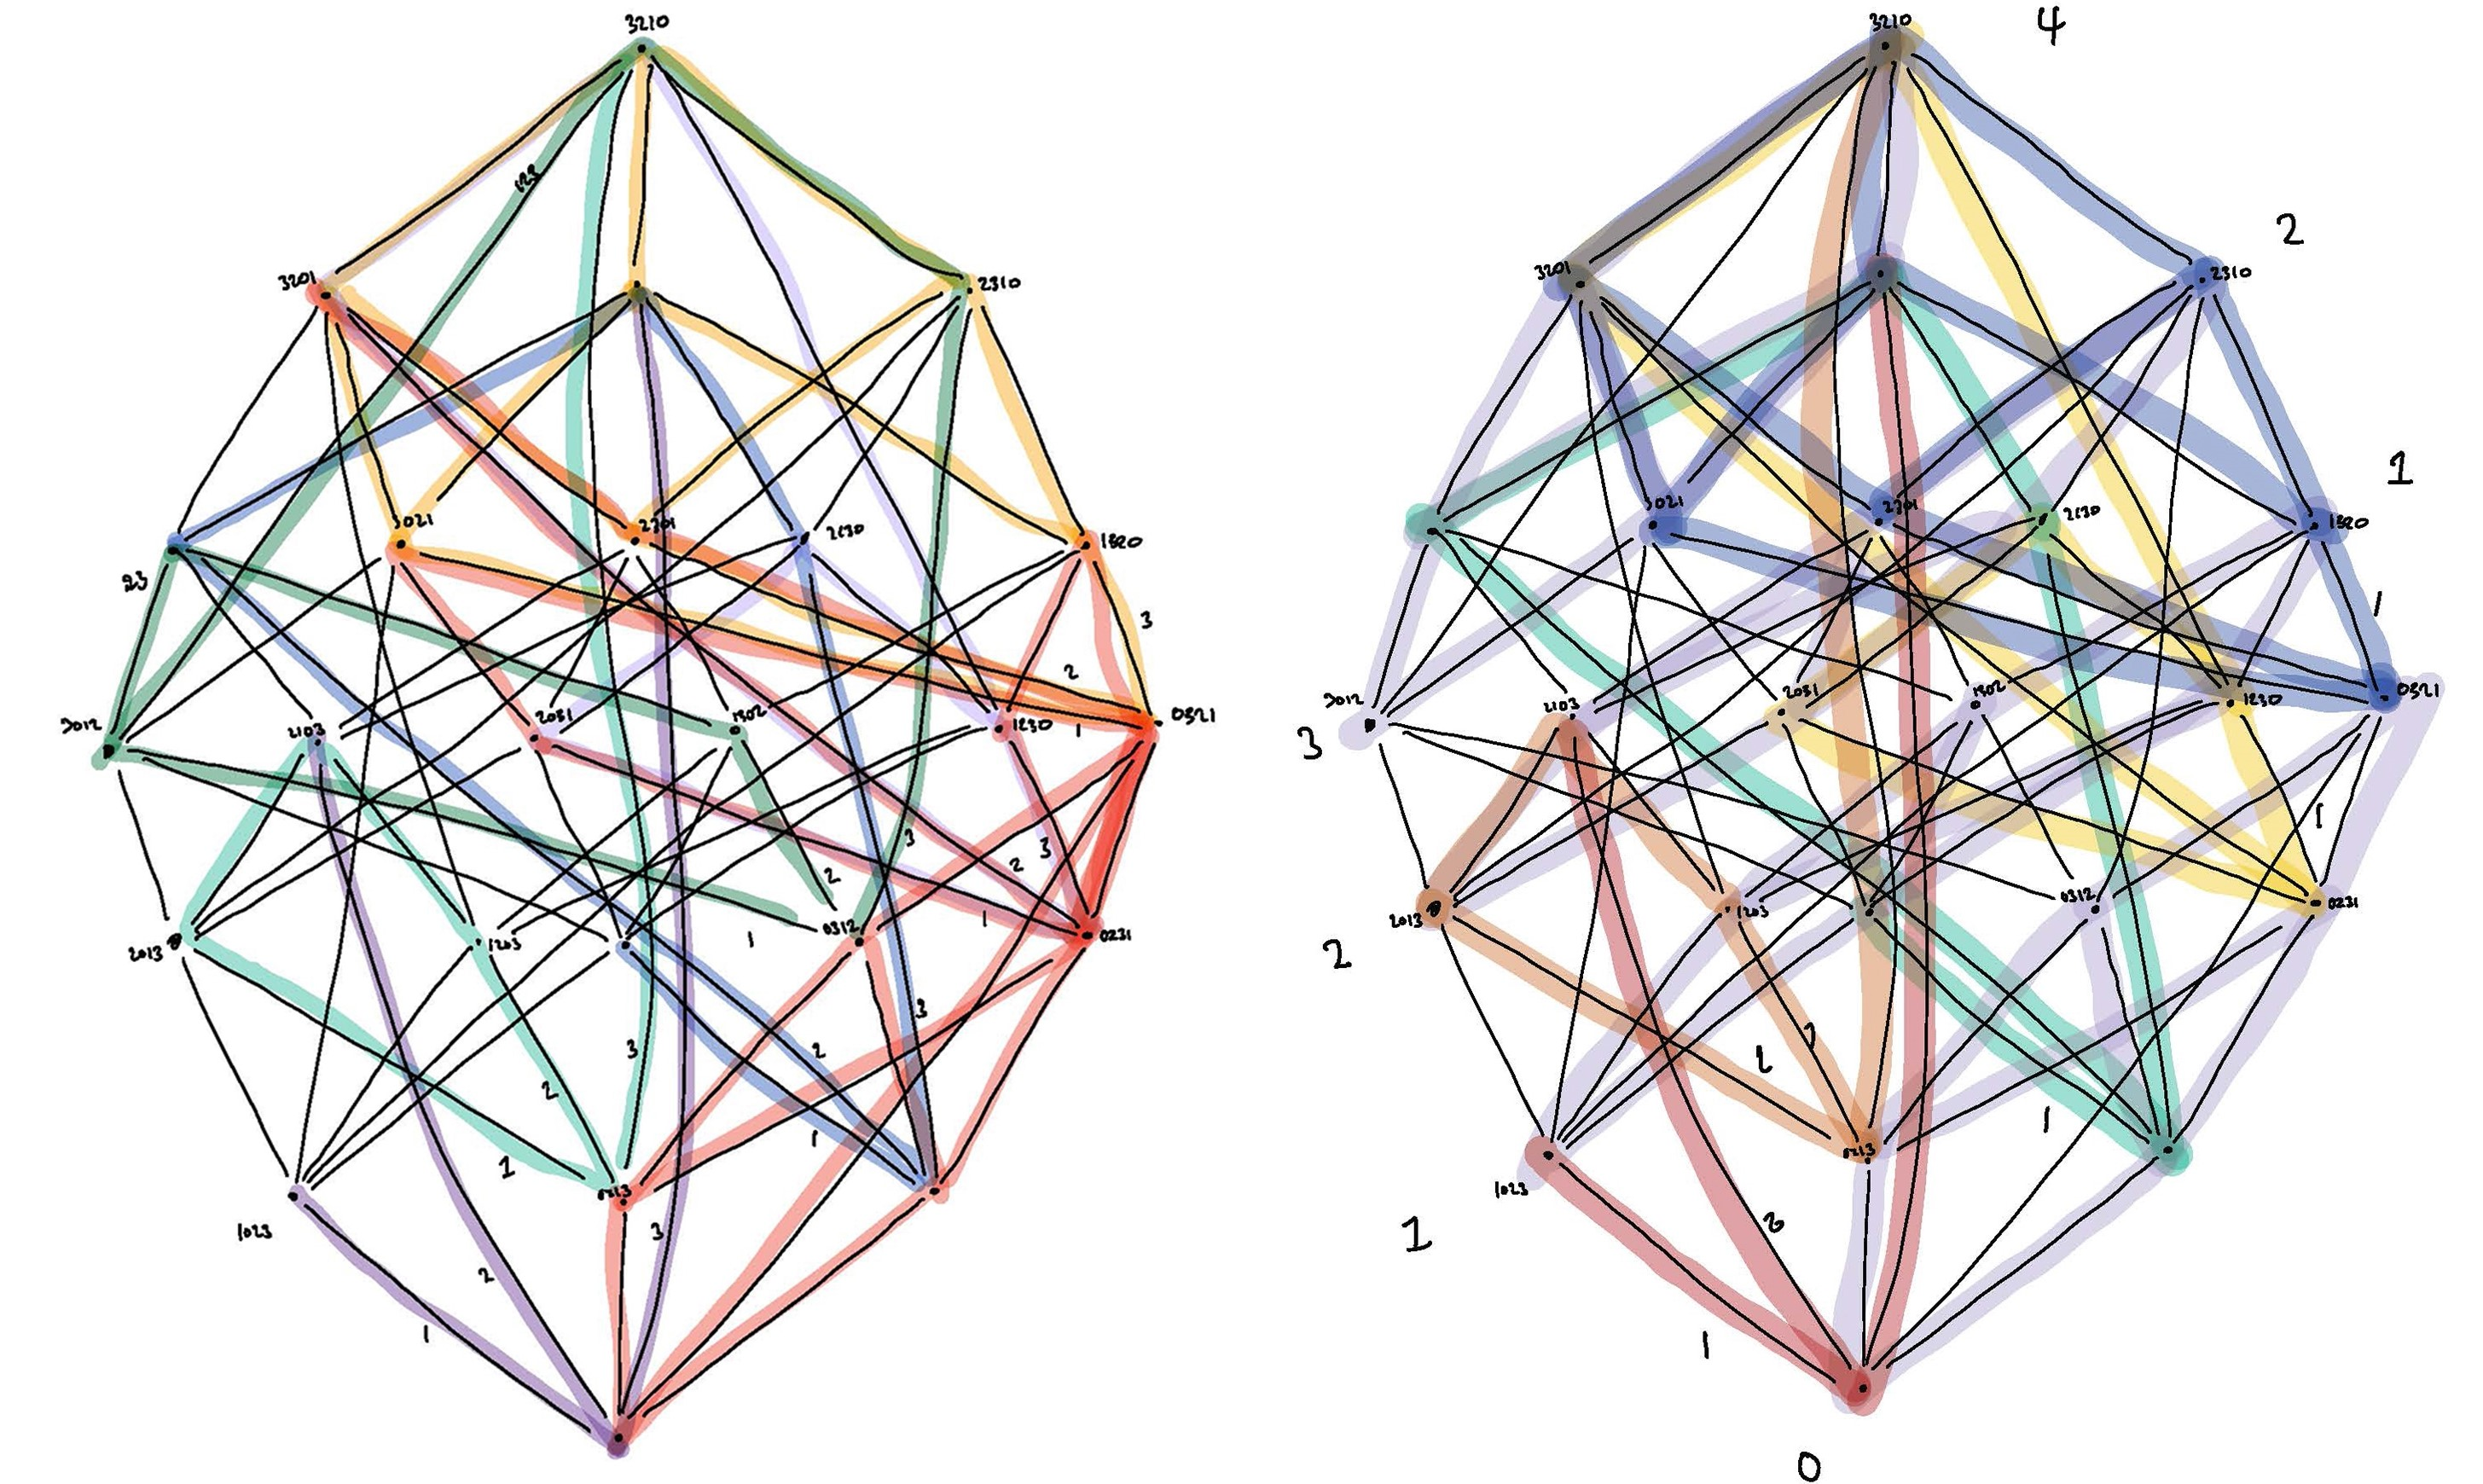
\includegraphics[width=0.85\linewidth]{5}
		\caption{\small\textit{\color{duongvaotoanhoc}Các nhà toán học và DeepMind đã sử dụng học máy để tìm kiếm công thức chuyển đổi đồ thị Bruhat thành đa thức.}}
		\vspace*{-10pt}
	\end{figure}
	Sau một thời gian ngắn, nó có thể thường xuyên dự đoán đúng đa thức Kazhdan--Lusztig từ đồ thị Bruhat. Nhưng để viết ra được cách thức chuyển từ cái này sang cái kia, Williamson cần biết máy tính đã đưa ra dự đoán của nó như thế nào.
	\vskip 0.05cm
	\textbf{\color{duongvaotoanhoc}Một công thức, nếu bạn có thể chứng minh nó}
	\vskip 0.05cm
	Ở đây, một lần nữa, các nhà nghiên cứu DeepMind đã sử dụng kỹ thuật xác định độ quan trọng. Đồ thị Bruhat rất lớn, nhưng các dự đoán của máy tính chủ yếu dựa trên một số lượng nhỏ các cạnh. Các cạnh biểu diễn các sự hoán đổi vị trí của các số cách xa nhau (như $1$ và $9$) có vai trò quan trọng trong việc dự đoán hơn là các cạnh kết nối các hoán vị đảo vị trí các số liền nhau (như $4$ và $5$). Đó là một manh mối mà Williamson sau đó phải phát triển thêm.
	\vskip 0.05cm
	Williamson kể lại: ``Alex [Davies] liên tục nói với tôi rằng những cạnh này, không hiểu vì lý do gì, quan trọng hơn rất nhiều so với những cạnh khác. Quả bóng  lại bay về sân  của tôi, và tôi đã nhìn chằm chằm vào chúng trong vài tháng."
	\vskip 0.05cm
	Sau đó Williamson nghĩ ra khoảng $10$ công thức chuyển đổi đồ thị Bruhat thành đa thức Kazhdan--Luzstig. Sau đó, nhóm nghiên cứu của DeepMind kiểm tra chúng trên hàng triệu ví dụ về đồ thị Bruhat. Đối với những công thức đầu tiên của Williamson, nhóm của DeepMind đã nhanh chóng tìm thấy các phản ví dụ -- và cho thấy các công thức đưa ra là không đúng.
	\vskip 0.05cm
	Nhưng cuối cùng Williamson đã tìm ra một công thức có vẻ phù hợp. Nó liên quan đến việc chia nhỏ đồ thị Bruhat thành các phần giống như hình khối và sử dụng thông tin đó để tính đa thức Kazhdan--Lusztig. Kể từ đó, các nhà nghiên cứu của DeepMind đã xác thực công thức đó trên hàng triệu ví dụ. Giờ đây, Williamson và các nhà toán học khác phải chứng minh công thức đó là đúng.
	\vskip 0.05cm
	Sử dụng máy tính để kiểm tra các ví dụ là một phần quen thuộc trong nghiên cứu toán học. Nhưng những hợp tác gần đây làm cho máy tính trở nên hữu ích theo một cách mới. Đối với các bài toán nặng về dữ liệu, học máy có thể giúp chỉ dẫn các nhà toán học theo những hướng mới, giống như một đồng nghiệp thường đưa ra một đề xuất vậy.
\end{multicols}
\vspace*{-10pt}
\rule{1\linewidth}{0.1pt}
\blfootnote{$^1$\color{duongvaotoanhoc}Trường Đại học KHTN, ĐHQG Hà Nội.}
\begingroup
\AddToShipoutPicture*{\put(124,480){
\includegraphics[scale=1]{../tieude.pdf}}}
\centering
\endgroup

\vspace*{76pt}

\textit{\textbf{\color{duongvaotoanhoc}LTS.} Tại Đại hội Toán học Thế giới năm $2022$ vừa qua, $4$ huy chương Fields đã được trao cho các nhà toán học Hugo Duminil--Copin, June Huh, James Maynard và Maryna Viazovska. Trong phần I của bài viết (xem Pi số $7-8/2022$), tác giả đã giới thiệu về những đóng góp tiêu biểu của  Hugo Duminil--Copin và James Maynard. Trong phần II, tác giả tiếp tục giới thiệu với bạn đọc những thành tựu nổi bật của June Huh và Maryna Viazovska.}
\begin{multicols}{2}	
	$3.$ June Huh: Anh được xem là đã cùng với một số cộng sự làm thay đổi lĩnh vực hình học tổ hợp thông qua việc dùng các phương pháp của lý thuyết Hodge (phương pháp để nghiên cứu đối đồng điều của những đa tạp Kahler compact), hình học nhiệt đới (tropical), và lý thuyết kỳ dị. Đối tượng tổ hợp chính mà June Huh quan tâm là các matroids. Matroid là một đối tượng gần với ma trận (matrix) và lý thuyết đồ thị, và lý thuyết về chúng có cảm hứng từ việc trừu tượng hóa nhiều khái niệm từ hai lý thuyết nói trên. Cụ thể hơn, matroid $M$ là một cặp $(E,\pazocal{I})$ gồm một tập hữu hạn $E$ và một họ $\pazocal{I}$ khác rỗng các tập con của $E$ thỏa mãn đồng thời $2$ điều kiện:
	\vskip 0.05cm
	$\bullet$ Nếu tập con $A$ của $E$ thuộc họ $\pazocal{I}$ thì mọi tập con của nó cũng thuộc $\pazocal{I}$.
	\vskip 0.05cm
	$\bullet$ Nếu $A, B \in \pazocal{I}$ và $|A| = |B| +1$, thì tồn tại một phần tử $x \in A \setminus B$ sao cho $B \cup \{x\} \in \pazocal{I}$.
	\vskip 0.05cm
	Mô hình cụ thể của một matroid là một ma trận với các cột đánh số bởi tập $E$ và họ $\pazocal{I}$ các tập con mà các cột ứng với tập con đó là độc lập tuyến tính.
	\vskip 0.05cm
	Đây là một khái niệm đưa ra bởi một nhà hình học nổi tiếng của thế kỷ trước là H. Whitney sau đó được phát triển nhiều bởi một chuyên gia nổi tiếng về tổ hợp là G--C. Rota. Sau này matroids tìm thấy nhiều ứng dụng trong hình học, tôpô, tổ hợp, ...
	\vskip 0.05cm
	Bên cạnh đó, hình học nhiệt đới (tropical) là một biến thể của hình học đại số. Trong khi hình học đại số nghiên cứu những đa tạp đại số là tập nghiệm của một hệ phương trình đa thức thì hình học nhiệt đới thay phép cộng trong đa thức bởi phép lấy giá trị nhỏ nhất và phép nhân thay bằng phép cộng. Ngay trong hình học đại số, lý thuyết hình học mới này đã có nhiều ứng dụng thông qua các công trình của M. Kontsevich (Huy chương Fields năm $1998$) và G. Mikhalkin. Tuy xuất phát từ hình học đại số nhưng theo nhận xét của June Huh các đa tạp nhiệt đới rộng hơn nhiều so với việc lấy nhiệt đới hóa (tropicalization) các đa tạp đại số, qua đó cho thấy những nghiên cứu của June Huh chắc sẽ còn hứa hẹn nhiều kết quả quan trọng.  
	\vskip 0.05cm
	Cụ thể hơn những công trình quan trọng làm nên Huy chương Fields của June Huh bao gồm:
	\vskip 0.05cm
	$\bullet$ June Huh đã cùng với Boton Wang sử dụng Hình học đại số và lý thuyết giao để chứng minh giả thuyết Dowling--Wilson về nhận biết các matroids. 
	\vskip 0.05cm
	$\bullet$ Karim Adiprasito, June Huh, và Eric Katz đã tìm ra một dạng tương tự của lý thuyết Hodge và chứng minh định lý Lefschetz dạng mạnh và quan hệ Hodge--Riemann cho các matroids tùy ý. Họ đã dùng các kết quả này để giải quyết giả thuyết Heron--Rota--Welsh về tính lõm loga của đa thức đặc trưng của một matroid. 
	\vskip 0.05cm
	$\bullet$ Petter Branden và June Huh đã phát triển lý thuyết về các đa thức Lorentz, liên hệ với giải tích lồi và phiên bản rời rạc của nó thông qua hình học nhiệt đới. Họ đã chứng minh giả thuyết Mason dạng mạnh cho các matroids và tìm ra các ứng dụng khác nhau từ hình học đại số xạ ảnh cho tới mô hình Potts trong cơ học thống kê (đã được đề cập đến trong công việc của Hugo Duminil--Copin).
	\vskip 0.05cm 
	June Huh có một quá trình đào tạo về Toán không thật chính quy. Anh tự nhận không giỏi Toán khi học phổ thông và học cả chuyên ngành Vật lý ở bậc đại học ở Đại học Quốc Gia Seoul (Hàn Quốc) nhưng bảng điểm không thật tốt. Đến những năm cuối đại học, anh được tham dự các bài giảng về Hình học đại số của H. Hironaka (Huy chương Fields năm $1970$ của Nhật Bản, nổi tiếng với định lý giải kỳ dị) khi ông là Giáo sư mời của Đại học Quốc gia Seoul. Lúc này anh bắt đầu có cảm hứng và bắt đầu dành nhiều thời gian hơn cho Toán học. Tốt nghiệp Đại học xong, anh làm luận văn Thạc sỹ với một trong những chuyên gia hàng đầu về Hình học đại số của Hàn Quốc là Young--Hoon Kiem. Sau đó, năm $2009$, anh được nhận làm luận án Tiến sỹ Toán ở Mỹ, ban đầu là Đại học Illinois ở Urbana--Champaign, sau đó chuyển sang Đại học Michigan. Anh bảo vệ luận án Tiến sỹ năm $2014$ dưới sự hướng dẫn của một chuyên gia nổi tiếng về Hình học đại số là M. Mustata. Tuy bắt đầu làm luận án Tiến sỹ khá muộn, nhưng ngay từ những năm đầu khi làm luận án Tiến sỹ, anh đã dùng những kỹ thuật của hình học đại số để chứng minh giả thuyết Read về hệ số của đa thức sắc số (chromatic polynomials) trong lý thuyết đồ thị. Đây là một giả thuyết từ hơn $40$ năm trước xuất phát từ bài toán $4$ màu nổi tiếng mà lời giải của nó dài vài trăm trang được đưa ra bởi K. Appel và W. Haken năm $1976$ cùng với sự hỗ trợ của máy tính. Bài báo của June Huh ngay lập tức đã được chú ý và in ở một tạp chí hàng đầu là Journal of the American Mathematical Society. Một điều thú vị là chính trong bài báo này, June Huh cũng đã trả lời một câu hỏi liên quan của GS. Ngô Việt Trung và J. K. Verma về số bội trộn trong Đại số giao hoán. Nhờ những kết quả quan trọng trong luận án, anh được nhận học bổng nghiên cứu danh giá của Viện Clay, và nhận vị trí Veblen Instructor, cũng như vị trí giáo sư mời ở Viện nghiên cứu cao cấp Princeton. Đến năm $2020$, anh nhận vị trí giáo sư ở Đại học Stanford, nhưng chỉ $1$ năm sau đó anh quay lại nhận vị trí giáo sư ở Đại học Princeton.     
	\vskip 0.05cm
	$4.$ Maryna Viazovska: Như đã nói ở phần I, Maryna Viazovska được trao huy chương Fields một phần vì những đóng góp trong bài toán xếp hình cầu.
	\vskip 0.05cm
	Một vấn đề có từ lâu trong toán học là tìm một cách sắp xếp dày đặc nhất (tối ưu nhất) những hình cầu giống nhau trong không gian với số chiều cho trước. Dày đặc nhất ở đây hiểu là tỷ lệ giữa tổng thể tích các hình cầu và thể tích hình chứa nó là lớn nhất. Bài toán này cũng rất tự nhiên trong thực tế khi ta đi du lịch và cần phải xắp xếp sao cho balo chứa được nhiều đồ vật nhất. Ở chiều $2$ ta biết cách sắp xếp theo hình lục lăng (một hình tròn ở giữa, $6$ hình tròn đặt xung quanh trong một lục giác đều) cho ta cách xếp dày đặc nhất. Với số chiều $3$, từ vài trăm năm trước, J. Kepler đã dự đoán cách xếp các quả cam chứa trong một hình kim tự tháp sẽ cho kết quả tối ưu. Năm $1998$, T. Hales chứng minh giả thuyết Kepler với một chứng minh gần $100$ trang in ở Annals of Mathematics cùng với sự trợ giúp của máy tính. Bài toán sắp xếp hình cầu không có thêm kết quả gì ở các số chiều khác cho đến năm $2016$, M.~Viazovska chỉ ra dàn $E_{8}$ (dàn (lưới) trong không gian $\mathbb{R}^8$, liên quan đến nhóm Lie dạng $E_{8}$) cho cách xếp tối ưu nhất trong chiều $8$. Ít lâu sau đó cùng với H. Cohn, A. Kumar, S. Miller và D. Radchenko, M.~Viazovska đã chứng minh dàn Leech cho cách sắp xếp dày đặc nhất ở số chiều $24$. Dàn Leech nằm trong không gian $\mathbb{R}^{24}$ có nhóm các tự đẳng cấu là nhóm đơn hữu hạn loại lẻ tẻ (sporadic) đưa ra bởi Conway. Lời giải của M.~Viazovska dựa trên cách tiếp cận của H. Cohn và N.~Elkies (Ann. Math. $2003$), những người đã dùng công thức tổng Poisson của giải tích điều hòa để tìm ra một chặn trên cho những khả năng có thể có của mật độ cho bài toán xếp cầu với số chiều tùy ý. Công trình của các nhà toán học này cần đến sự tồn tại của những hàm Schwatz với những tính chất đặc biệt (chẳng hạn hàm đó và biến đổi Fourier của nó triệt tiêu tại những giá trị độ dài của vectơ trong các dàn tương ứng). H. Cohn và N.~Elkies nghĩ rằng những hàm có tính chất đặc biệt như thế là tồn tại nhưng chưa có ý tưởng gì để xây dựng. Khi công việc dừng ở đó khoảng $10$ năm thì M.~Viazovska xuất hiện và đưa ra một phương pháp hoàn toàn mới để đưa ra những hàm này dựa trên lý thuyết về các dạng modular. Như chúng ta đã biết các dạng modular là một lĩnh vực thuộc Lý thuyết số hiện đại và cung cấp những điểm mấu chốt cho lời giải bài toán Fermat của A. Wiles từ khoảng gần $30$ năm trước. Sau đó kỹ thuật chọn hàm Schwatz dùng dạng modular cũng đã được H. Cohn khai thác và thu được những kết quả quan trọng gần đây. Việc dùng các dạng modular là một đối tượng rất khác để giải quyết vấn đề nói trên ít nhiều có sự hợp lý nếu chúng ta nhìn vào đào tạo của M.~Viazovska. Ngay từ phổ thông, chị đã là một học sinh giỏi Toán, tốt nghiệp Đại học ở Ucraina, sau đó làm luận văn cao học Đức, rồi quay lại Ucraina làm luận án Tiến sỹ và bảo vệ vào năm $2010$. Sau đó chị sang Đức làm luận án Tiến sỹ với một trong hai người thầy hướng dẫn là Don Zagier, một chuyên gia về nhiều thứ trong đó có lý thuyết các dạng modular. Một điều đáng ngạc nhiên là mặc dù lời giải bài toán xếp cầu trong trường hợp $3$ chiều rất dài và cần đến máy tính kiểm tra nhưng lời giải trong trường hợp $8$ chiều và $24$ chiều lại khá ngắn gọn (khoảng $20$ trang). Vì những kết quả độc đáo này, M.~Viazovska đã nhận được giải thưởng nghiên cứu của Viện Clay năm $2017$ dành cho những kết quả Toán học xuất sắc nhất trong năm.        
	\vskip 0.05cm
	Sau lời giải bài toán xếp cầu ở chiều $8$ và $24$, M.~Viazovska đã phát triển tiếp tục ý tưởng của riêng mình. Chị đã cùng với D.~Radchenko ($2019$) chứng minh mọi hàm Schwatz chẵn thỏa mãn hàm đó cùng với biến đổi Fourier triệt tiêu tại các số $\sqrt{n}$ ($n$ là số nguyên không âm) luôn đồng nhất bằng $0$. Kết quả này được các chuyên gia đánh giá là rất đáng ngạc nhiên.
	\vskip 0.05cm
	{\bf\color{duongvaotoanhoc} Kết luận:}  Từ những phân tích kể trên ta thấy đóng góp của những giải thưởng Fields luôn rất đặc biệt, thường là lời giải cho những vấn đề quan trọng, và lời giải nhiều khi đến từ những lĩnh vực hoàn toàn khác.
	\vskip 0.05cm
	\textbf{\color{duongvaotoanhoc}Tài liệu tham khảo}
	\vskip 0.05cm
	[$1$] Trang web {\color{duongvaotoanhoc}https://www.mathunion.org/\\imu-awards/fields-medal/fields-medals-2022}
	\vskip 0.05cm
\end{multicols} 
	\newpage
	
	 \setcounter{figure}{0}
	 \thispagestyle{quantoannone}
\pagestyle{quantoan}
\everymath{\color{quantoan}}
\graphicspath{{../quantoan/pic/}}
\blfootnote{\color{quantoan}\color{quantoan}$^1$Viện Toán học.}
\begingroup
\AddToShipoutPicture*{\put(0,616){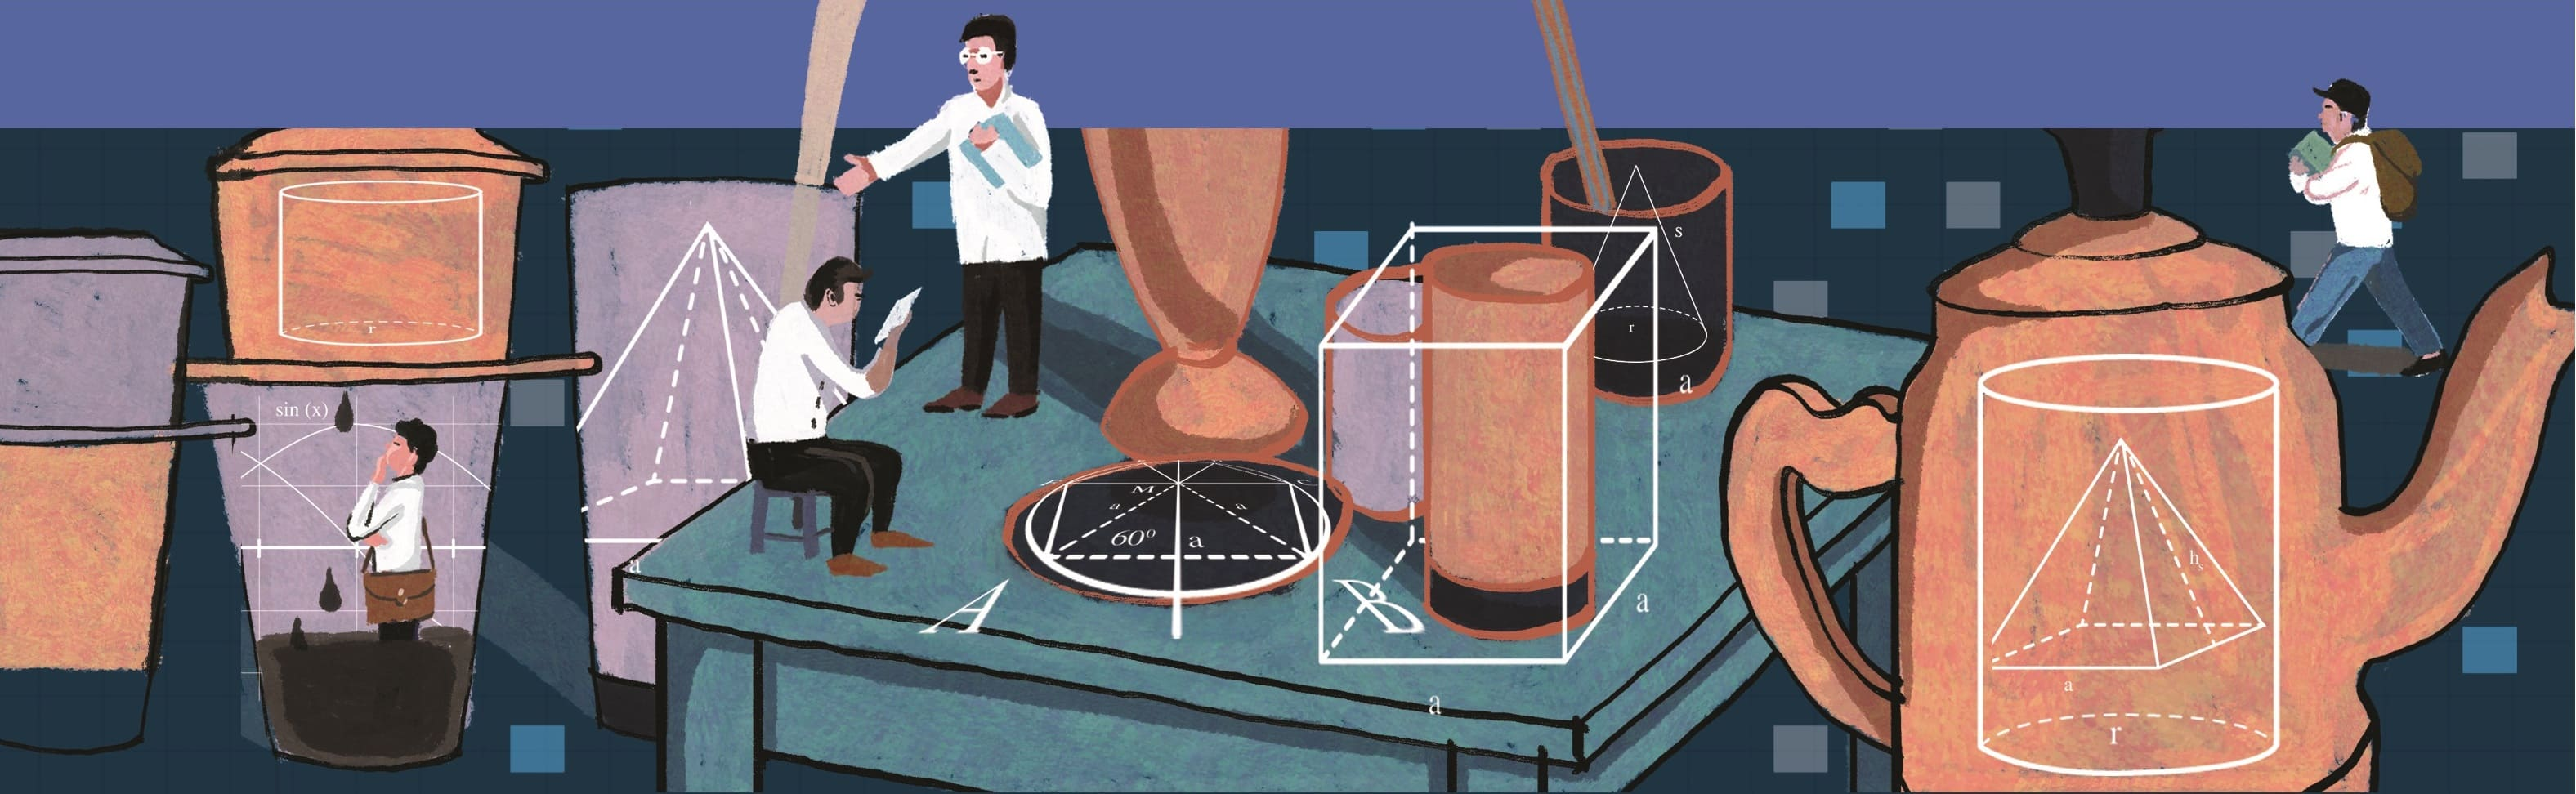
\includegraphics[width=19.3cm]{../bannerquantoan}}}
\AddToShipoutPicture*{\put(70,550){
\includegraphics[scale=1]{../tieude11.pdf}}}
\centering
\endgroup

\vspace*{160pt}

\begin{multicols}{2}	
	Phép quy nạp dựa trên nguyên lý đơn giản: ta có thể tuần tự đếm được tất cả các số tự nhiên, bắt đầu từ $1$, rồi $2$, $3$, vân vân. Mặc dù ta không thể đếm được vô hạn lần, nhưng về nguyên tắc, nếu cố định một số tự nhiên, sớm hay muộn ta cũng sẽ đếm đến nó. Ta nói, tập số tự nhiên là đếm được. Bạn đọc cần phân biệt giữa ``đếm được" và ``đếm hết được nhé". Tất nhiên chúng ta không thể đếm hết được các số tự nhiên. Đếm được là cách chúng ta kiểm soát các số tự nhiên -- tuy toàn thể chúng là vô hạn, nhưng từng phần tử lại có thể đạt tới sau một quy trình hữu hạn. 
	\vskip 0.1cm
	Liệu tập các số hữu tỷ có đếm được không? Nếu hình dung các số hữu tỷ như là những điểm trên trục số, ta thấy chúng thật dày đặc. Chỉ trong khoảng giữa số $0$ và số $1$ thôi, đã có vô hạn số hữu tỷ rồi, làm sao đếm hết được!?
	\vskip 0.1cm
	Câu trả lời hóa ra là ``có" các bạn ạ. Đương nhiên, ta sẽ không đếm hết tất cả các số hữu tỷ trong khoảng $0$ đến $1$ trước rồi mới đếm tiếp các số trong khoảng $1$ đến $2$. Bởi ta không thể ``đếm hết" các số trong khoảng $0$ đến $1$. Thay vào đó, ta sẽ chọn trong mỗi khoảng một vài số để đếm dần dần, vừa ``sâu" vào trong từng khoảng đồng thời ``rộng" sang các khoảng khác. 
	\vskip 0.1cm
	Đây là một ``mẹo" rất thông minh, tác giả của nó có lẽ là Cantor. Ta sẽ biểu diễn số hữu tỷ dưới dạng phân số tối giản $\dfrac{p}{q}$, với $p$, $q$ là các số nguyên dương (để đơn giản ta sẽ chỉ đếm các số hữu tỷ dương, bạn đọc tự xây dựng cách đếm tất cả các số hữu tỷ nhé). Ta sẽ đếm dần theo cả tử số lẫn mẫu số. Bắt đầu là $\dfrac{1}{1}$, rồi $\dfrac{2}{1}$, $\dfrac{1}{2}$, rồi $\dfrac{3}{1}$, $\dfrac{1}{3}$, rồi $\dfrac{4}{1}$, $\dfrac{3}{2}$, $\dfrac{2}{3}$, $\dfrac{1}{4}$,rồi $\dfrac{5}{1}$, $\dfrac{1}{5}$, ... cứ như thế, những phân số không tối giản (ví dụ $\dfrac{2}{2}$, $\dfrac{4}{2}$,...) sẽ bị bỏ qua. Tử cùng mẫu sẽ lớn dần, tất cả các phân số tối giản sẽ được đếm, nghĩa là tất cả các số hữu tỷ (dương) sẽ được đếm. 
	\vskip 0.1cm
	Hình dung các số này trên trục số ta thấy, một mặt, các số trên khoảng $(0,1)$ sẽ được đếm ngày càng nhiều, mặt khác, mỗi bước ta lại đếm rộng ra các số trên những khoảng khác, mỗi ngày một xa. 
	\vskip 0.1cm
	Câu hỏi tiếp theo tất nhiên là về các số thực. Liệu tập số thực có đếm được không? 
	\vskip 0.1cm
	Để có thể đếm số thực, câu hỏi đầu tiên là: số thực là gì? Có lẽ các bạn ngạc nhiên bởi câu hỏi, bởi đã là số (có) thực, lại còn hỏi nó là gì! 
	\vskip 0.1cm
	Nhưng số thực là gì?
	\vskip 0.1cm
	Ta biết ví dụ về các số thực, như các số tự nhiên $1,2,3,4, \ldots$; hay các số hữu tỷ; rồi các số vô tỷ, như $\pi, e,\ldots$ Nhưng thế nào là một số thực, làm thế nào để biểu diễn một số thực?
	\end{multicols}
	\begin{figure}[H]
		\vspace*{5pt}
		\centering
		\captionsetup{labelformat= empty, justification=centering}
		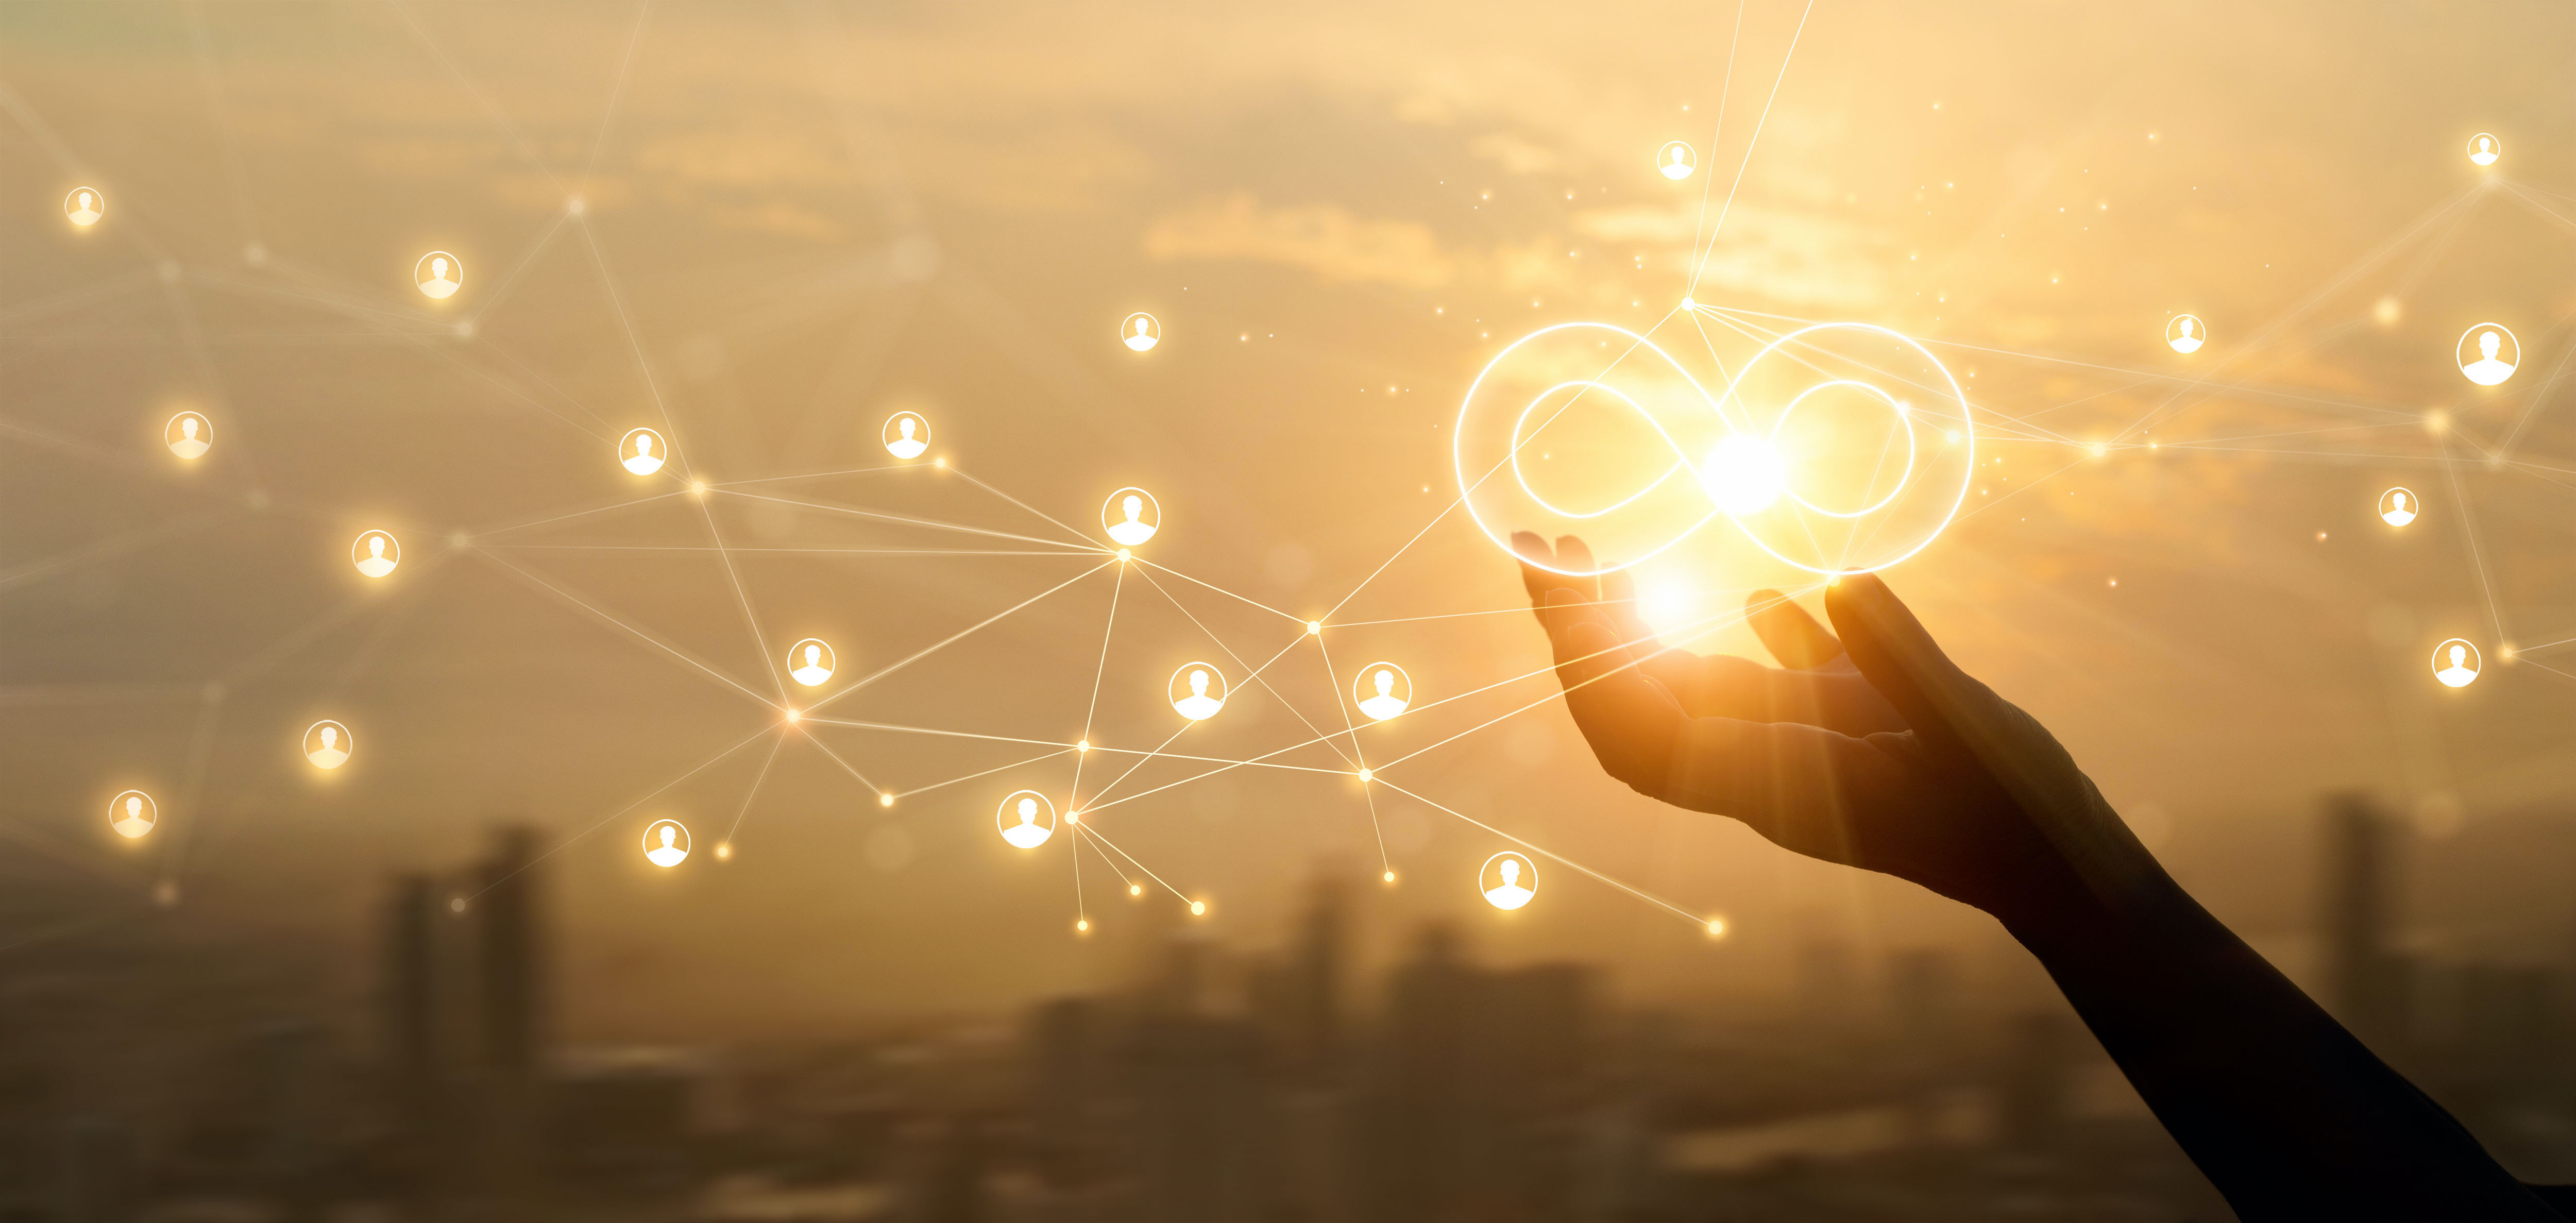
\includegraphics[width= 1\linewidth]{1a}
		\vspace*{-10pt}
	\end{figure}
	\begin{multicols}{2}
	Chúng ta sẽ thảo luận về số thực trong một bài viết sau. Để kết thúc bài viết này, tôi sẽ chỉ ra ví dụ một tập hợp không đếm được: tập các tập con của tập các số tự nhiên.
	\vskip 0.1cm
	Gọi $P_N$ là tập các tập con của tập các số tự nhiên. Như vậy, một phần tử của $P_N$ có thể là một tập hữu hạn các số tự nhiên, hoặc cũng có thể là một tập vô hạn. Thông thường ta mô tả chúng như những dãy số -- có hữu hạn hoặc vô hạn số hạng. 
	\vskip 0.1cm
	Ta sẽ chứng minh bằng phản chứng. Giả sử $P_N$ là đếm được, như vậy ta có thể sắp các phần tử của $P_N$ thành một dãy:
	\begin{align*}
		A_0, A_1, \ldots, A_k, \ldots,
	\end{align*}
	trong đó mỗi phần tử $A_k$ là một tập con của $P_N$ và mỗi tập con của $P_N$ sẽ xuất hiện như một phần tử $A_k$ ở dãy trên.
	\vskip 0.1cm
	Như vậy, với mỗi số tự nhiên $k$ sẽ có hai khả năng, hoặc nó là phần tử của $A_k$ hoặc nó không là phần tử của $A_k$. Gọi $B$ là tập hợp các số tự nhiên $k$ sao cho $k$ không là phần tử của $A_k$.
	\vskip 0.1cm
	Theo giả thiết ở trên thì $B$ sẽ xuất hiện trên dãy $(*)$ ở một vị trí nào đó, nghĩa là 
	$B=A_i$, với $i$ là một số tự nhiên nào đó.
	\vskip 0.1cm
	Các bạn có thấy điều gì vô lý không?
	Như các bạn có thể đã liên hệ với nghịch lý về sự tồn tại của ``tập tất cả các tập hợp", ở đây cũng xảy ra mâu thuẫn tương tự:
	\vskip 0.1cm
	-- $i$ không là phần tử của $B=A_i$, bởi theo giả thiết $B$ chỉ chứa những số $k$ mà $k$ không thuộc $A_k$;
	\vskip 0.1cm
	-- nếu $i$ không là phần tử của $A_i$ thì cũng theo giả thiết, $i$ thuộc $B=A_i$.
	\vskip 0.1cm
	Mâu thuẫn chứng tỏ giả thiết phản chứng của ta là sai (bạn nào chưa hiểu thế nào là chứng minh phản chứng thì xem thêm bài viết về Quy nạp nhé). Vậy ta có điều phải chứng minh: không thể liệt kê hết được các tập hợp con của tập các số tự nhiên thành một dãy, nói cách khác, tập $P_N$ các tập con của tập các số tự nhiên là không đếm được.
	\vskip 0.1cm
	Bạn đọc có thể thấy rằng chứng minh ở trên có thể lặp lại đối với một tập hợp $X$ bất kỳ để chứng minh không tồn tại một song ánh từ $X$ tới $P_X$ -- tập các tập con của $X$.
	%		\begin{figure}[H]
		%		\centering
		%		\vspace*{-5pt}
		%		\captionsetup{labelformat= empty, justification=centering}
		%		
\includegraphics[width=0.5\linewidth]{4}
		%		\vspace*{-5pt}
		%	\end{figure}
\end{multicols}
%\vspace*{-10pt}
%\rule{1\linewidth}{0.1pt}
%\begin{center}
%	\textbf{\LARGE\color{quantoan}LỜI GIẢI, ĐÁP ÁN}
%\end{center}
%
%\begin{multicols}{2}
%	\textbf{\color{quantoan}Quấy rầy thám tử}
%	\vskip 0.1cm
%	Vinh và Sinh không thể cùng nói dối, như vậy trong số họ phải có một người nói thật. Vì thế Du phải là người nói dối, khi khẳng định rằng cậu ta không làm vỡ kính. Vậy người làm vỡ kính là Du.
%	\vskip 0.1cm
%	\textbf{\color{quantoan}Đố vui}
%	\vskip 0.1cm
%	Đánh số các quả cân từ $1$ đến $6$. 
%	\vskip 0.1cm
%	Trước hết cân $1$ với $2$. Giả sử chúng nặng bằng nhau. Ở lần cân thứ hai, ta cân $1$ với $3$. Nếu chúng nặng bằng nhau thì $1$, $2$, $3$ là các quả cân nặng bằng nhau (cũng như $4$, $5$ và $6$). Do đó ở lần cân thứ $3$ ta chỉ cần so sánh $1$ và $4$ để xác định được những quả cân nào là đúng và những quả cân nào là sai. Nếu không, chẳng hạn $1$ nặng hơn $3$ (trường hợp $1$ nhẹ hơn $3$ tương tự), thì các quả cân $1$ và $2$ là các quả cân đúng và quả cân $3$ là quả cân sai. Bây giờ, trong số các quả cân $4$, $5$, $6$ có một quả cân đúng và hai quả cân sai. Để xác định, ta chỉ cần cân $4$ với $5$: nếu chúng nặng bằng nhau thì nghĩa là $4$ chúng là các quả cân sai; nếu không, quả nặng hơn là quả cân đúng (còn hai quả còn lại là quả cân sai). 
%	\vskip 0.1cm
%	Bây giờ, giả sử $1$ nặng hơn $2$ (trường hợp ngược lại tương tự), nghĩa là quả cân $1$ là đúng và quả cân $2$ là sai. Ở lần cân thứ hai, ta cân $1$ với $3$ để xác định được $3$ là quả cân đúng hai sai. Như vậy, sau $2$ lần cân, ta xác định được ba quả cân $1$, $2$, $3$: gồm hai quả đúng và một quả sai hoặc hai quả sai và một quả đúng. Ở lần cân cuối cùng, ta tiến hành như ở trường hợp bên trên, bằng cách cân $4$ với $5$, để xác định được những quả cân nào đúng và quả cân nào sai.  
%	\vskip 0.1cm
%	\hfill(\textit{Xem tiếp trang $36$})	
%		\textbf{Góc cờ}
%		\vskip 0.1cm
%		Hình $4$: $\pmb{1)}$	M$6.7$ Tg$4.1$\quad $\pmb{2)}$ C$5-6$ M$5.3$\quad $\pmb{3)}$ M$7/5$ Tg$4/1$\quad $\pmb{4)}$ C$6.1$ Tg$4-5$\quad $\pmb{5)}$ Tg$5-4$ T$7.9$\quad $\pmb{6)}$ C$6.1$ M$3.4$\quad $\pmb{7)}$ M$5.7$ ($1-0$)
%		\vskip 0.1cm
%		Hình $5$: $\pmb{1)}$ X$1-5$ M$8/7$\quad $\pmb{2)}$ X$5.1$ Tg$5/1$\quad $\pmb{3)}$ X$5-3$ Tg$5-4$\quad $\pmb{4)}$ X$3-6$ Tg$4-5$\quad $\pmb{5)}$ X$6.1$ Tg$5.1$\quad $\pmb{6)}$ X$6-8$ Tg$5-4$\quad $\pmb{7)}$ X$8.1$ Tg$4/1$\quad $\pmb{8)}$ X$8-5$ ($1-0$)
%\end{multicols}
	 \newpage

	 \setcounter{figure}{0}
	 \thispagestyle{toancuabinone}
\pagestyle{toancuabi}
\everymath{\color{toancuabi}}
\blfootnote{$^1$\color{toancuabi}Đại học Thăng Long.}
\graphicspath{{../toancuabi/pic1/}}
\begingroup
\AddToShipoutPicture*{\put(0,616){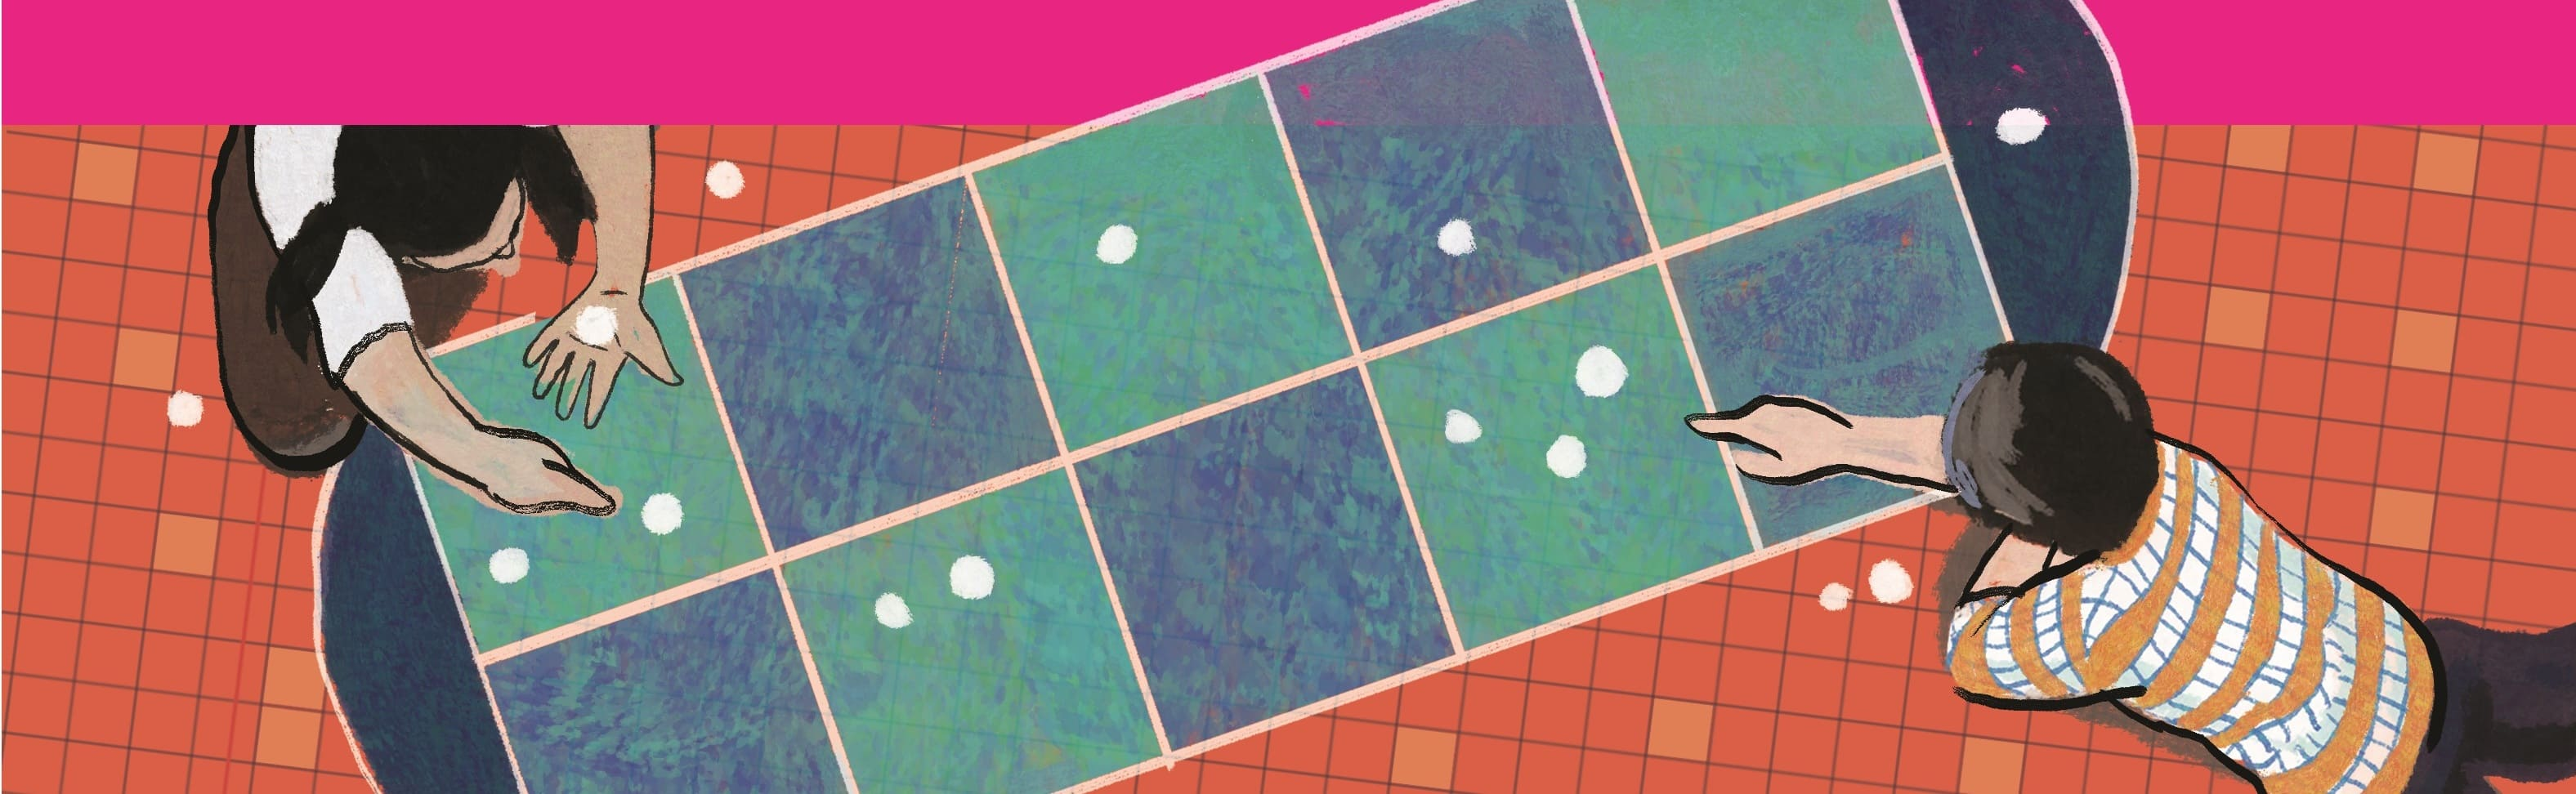
\includegraphics[width=19.3cm]{../bannertoancuabi}}}  
\AddToShipoutPicture*{\put(104,525){
\includegraphics[scale=1]{../tieude1.pdf}}} 
\centering
\endgroup
\vspace*{185pt}


\begin{multicols}{2}
	Trong phần $1$ của bài viết, các em đã được giới thiệu về số tượng hình của người Ai Cập cổ và cách ghi số của người La Mã dựa trên một số chữ cái trong bảng chữ cái. Trong phần $2$ này, chúng ta sẽ cùng tìm hiểu về số Babylon, số Maya và số Trung Hoa cổ.
	\vskip 0.1cm
	\textbf{\color{toancuabi}Số Babylon}
	\vskip 0.1cm
	Người Babylon, sống vào khoảng $5000$ năm trước ở vùng đất Lưỡng Hà (một khu vực ở phía Tây của  Châu Á). Họ đã tạo ra những công cụ tính toán thiên văn, hình học đáng kinh ngạc và họ đã phát minh ra bàn tính.
		\begin{figure}[H]
		\centering
		\vspace*{-5pt}
		\captionsetup{labelformat= empty, justification=centering}
		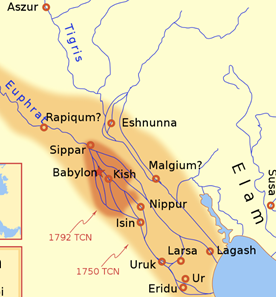
\includegraphics[width=1\linewidth]{17.1}
		\vspace*{-15pt}
	\end{figure}
	Để ghi số, ban đầu người Babylon chỉ sử dụng hai ký hiệu 
	\begin{table}[H]
		\vspace*{-5pt}
		\centering
		\begin{tabular}{|c|c|}
			\hline
			& \\[-2.5ex]
			
\includegraphics[scale=0.7]{15}&$1$\\
			\hline
			& \\[-2.5ex]
			
\includegraphics[scale=0.65]{16}&$10$\\
			\hline
		\end{tabular}
		\vspace*{-5pt}
	\end{table}
	để viết số từ $1$ tới $60$, chẳng hạn số $7$ là  
\includegraphics[scale=0.7]{17}, số $27$ là  
\includegraphics[scale=0.7]{16}
\includegraphics[scale=0.7]{16}
\includegraphics[scale=0.7]{17}. 	 
	\vskip 0.1cm
	Những ký hiệu này được sử dụng tương tự như những chữ số La Mã (bằng cách cộng các ký hiệu xuất hiện trong số được biểu diễn). Số 
\includegraphics[scale=0.7]{18} được viết bởi $2$ ký hiệu 
\includegraphics[scale=0.7]{16} để biểu diễn $2$ chục, và $7$ ký hiệu 
\includegraphics[scale=0.7]{15}  cho $7$ đơn vị. Do vậy 
\includegraphics[scale=0.7]{18}  $=27$.
	\vskip 0.1cm
	Sau đó, một ký hiệu mới được sử dụng để biểu diễn chữ số $0$ đó là:
	
\includegraphics[scale=0.65]{15.1}
	\vskip 0.1cm
	Để viết những số từ $60$ trở đi, người Babylon xếp các ký hiệu theo các nhóm. Điều này giống như ngày nay các bạn viết $159$ bằng cách viết số $1$ đầu tiên ứng với hàng trăm, số $5$ tiếp theo ở hàng chục và cuối cùng là số $9$ ở hàng đơn vị. Như vậy $159 = 1 \times 100+ 5 \times 10+ 9$.
	\vskip 0.1cm
	Để viết số $63$, người Babylon viết ký hiệu  
\includegraphics[scale=0.7]{15}  ở hàng $60$ và ba ký hiệu 
\includegraphics[scale=0.7]{15}  ở hàng đơn vị và để khoảng trống để phân biệt hai nhóm.
	\vskip 0.1cm
	
\includegraphics[scale=0.7]{16.1}$=63$. Trong cách viết này, ta thấy có $4$ ký hiệu 
\includegraphics[scale=0.7]{15}   nhưng ký hiệu đầu tiên được viết tách biệt so với $3$ cái còn lại để biểu diễn $1$ lần $60$ tức $60$, $3$ ký hiệu còn lại biểu diễn số $3$, và như vậy ta có số $60+3 =63$.
	\vskip 0.1cm
	Điều này giống như chúng ta viết chữ số $1$ ở hàng chục và chữ số $1$ ở hàng đơn vị để biểu diễn số $11$: nó có nghĩa là $1$ chục và $1$ đơn vị. Trong  cách ghi số  Babylon cổ, nó có nghĩa là $1$ lần $60$  và $1$.
	\begin{figure}[H]
		\centering
		\vspace*{-5pt}
		\captionsetup{labelformat= empty, justification=centering}
		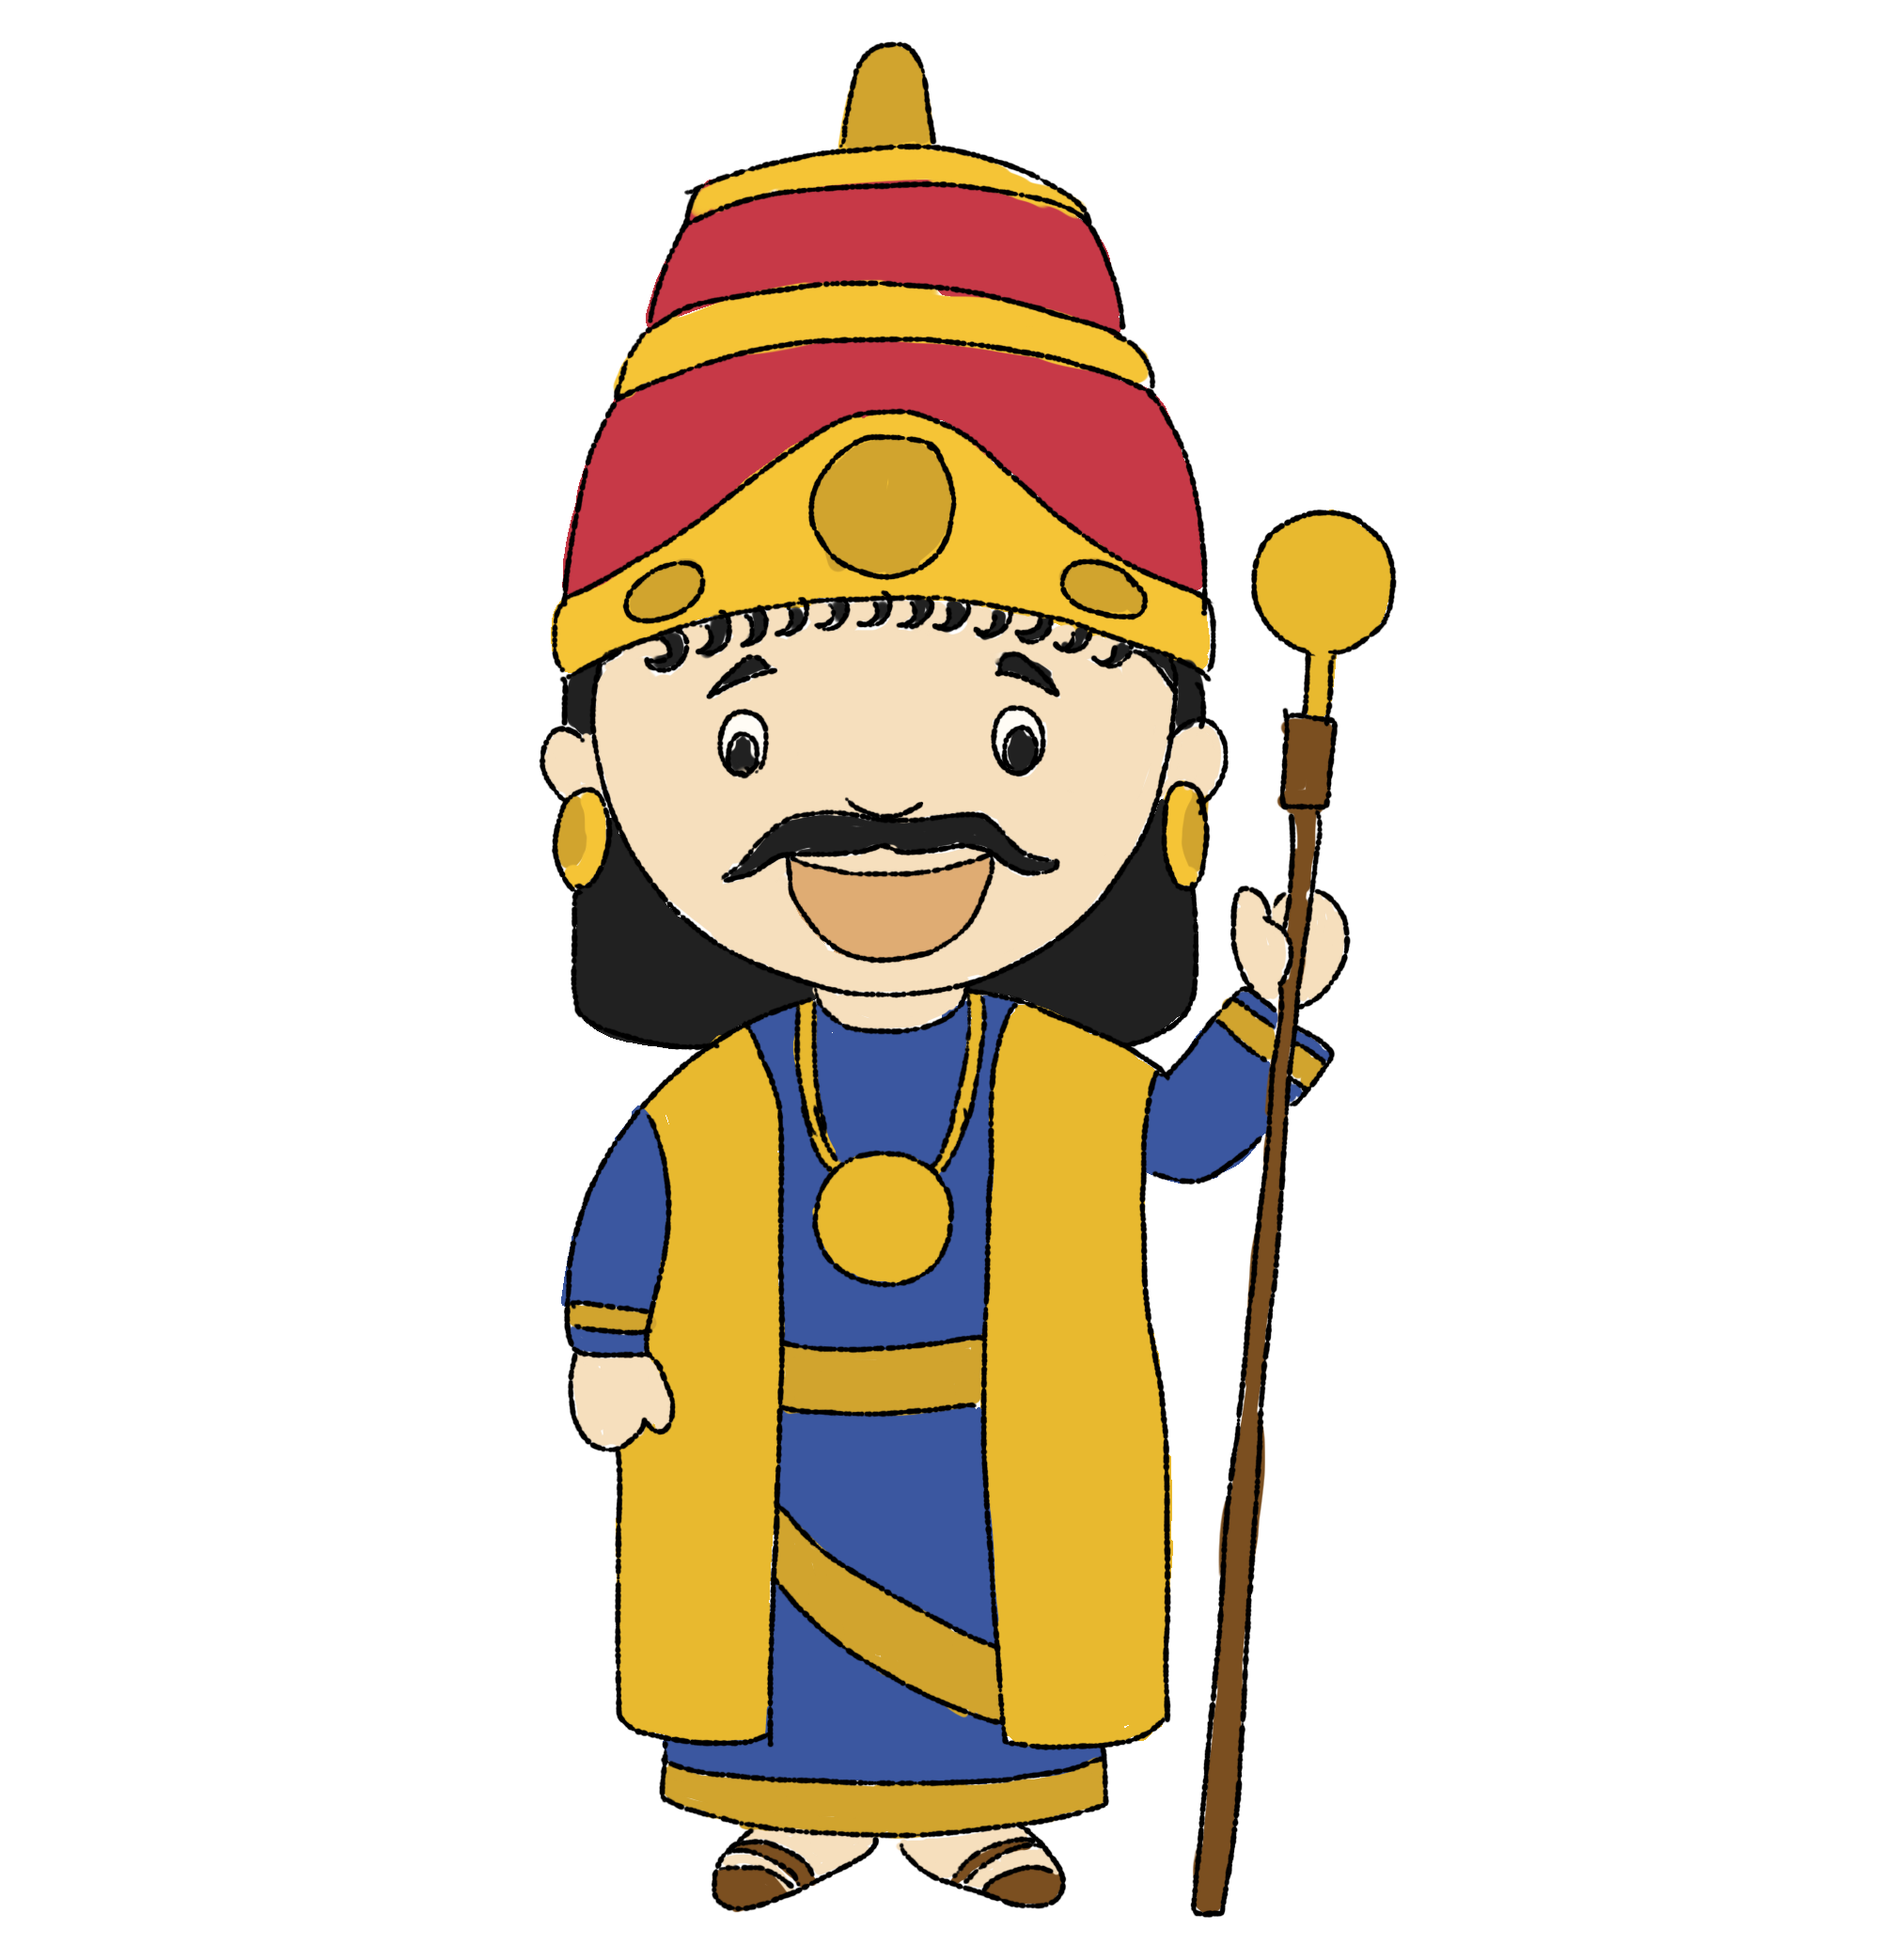
\includegraphics[width=0.85\linewidth]{20.12-pi.2}
		\vspace*{-15pt}
	\end{figure}
	Để hiểu rõ hơn, ta hãy viết số chín mươi ba theo cách ghi số hiện nay. Việc này thật dễ dàng phải không? Tuy nhiên để hiểu cách viết của người Babylon, ta sẽ thực hiện theo cách như sau: do chúng ta sử dụng hệ cơ số $10$, ta chia chín mươi ba cho $10$ được thương là $9$, nên ta viết $9$ vào hàng chục
	\begin{figure}[H]
		\centering
		\vspace*{-5pt}
		\captionsetup{labelformat= empty, justification=centering}
		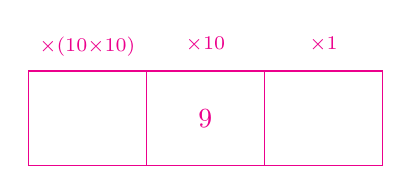
\begin{tikzpicture}[xscale=1.5,yscale=1.2,color=toancuabi]
			\draw (0,0) grid (3,1);
			\draw (1.5,0.5) node {$9$};
			\draw (0.5,1.05) node[above] {$\scriptstyle\times(10\times10)$};
			\draw (1.5,1.1) node[above] {$\scriptstyle\times10$};
			\draw (2.5,1.1) node[above] {$\scriptstyle\times1$};
		\end{tikzpicture}
		\vspace*{-10pt}
	\end{figure}
	Phép chia đó có số dư $3$ nên ta viết $3$ vào hàng đơn vị
	\begin{figure}[H]
		\centering
		\vspace*{-5pt}
		\captionsetup{labelformat= empty, justification=centering}
		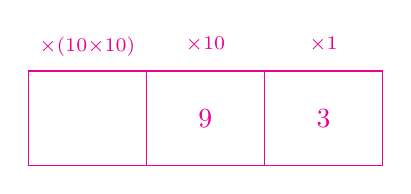
\begin{tikzpicture}[xscale=1.5,yscale=1.2,color=toancuabi]
			\draw (0,0) grid (3,1);
			\draw (1.5,0.5) node {$9$};
			\draw (2.5,0.5) node {$3$};
			\draw (0.5,1.05) node[above] {$\scriptstyle\times(10\times10)$};
			\draw (1.5,1.1) node[above] {$\scriptstyle\times10$};
			\draw (2.5,1.1) node[above] {$\scriptstyle\times1$};
		\end{tikzpicture}
		\vspace*{-10pt}
	\end{figure}
	Vậy là ta viết: $93$.
	\vskip 0.1cm
	Số chín mươi ba được viết như thế nào với số Babylon?
	\vskip 0.1cm
	Do cách ghi số Babylon sử dụng hệ cơ số $60$, ta chia $93$ cho $60$ được thương là $1$ nên ta viết $1$ ở hàng $60$.
	\begin{figure}[H]
		\centering
		\vspace*{-5pt}
		\captionsetup{labelformat= empty, justification=centering}
		\begin{tikzpicture}[xscale=1.5,yscale=1.2,color=toancuabi]
			\draw (0,0) grid (3,1);
			\node[inner sep=0pt] (mouse) at (1.5,0.5){
\includegraphics[scale=1]{27a.png}};
			\draw (0.5,1.05) node[above] {$\scriptstyle\times(60\times60)$};
			\draw (1.5,1.1) node[above] {$\scriptstyle\times60$};
			\draw (2.5,1.1) node[above] {$\scriptstyle\times1$};
		\end{tikzpicture}
		\vspace*{-10pt}
	\end{figure}
	Phép chia có số dư là $33$, nên ta sẽ viết $33$ ở hàng đơn vị. Số $33$ được biểu diễn bởi $3$ ký tự mười cộng với $3$. Nên ta đặt $3$ ký tự 
\includegraphics[scale=0.65]{16} và $3$ ký tự 
\includegraphics[scale=0.65]{15} vào hàng đơn vị như sau
	\begin{figure}[H]
		\centering
		\vspace*{-5pt}
		\captionsetup{labelformat= empty, justification=centering}
		\begin{tikzpicture}[xscale=1.5,yscale=1.2,color=toancuabi]
			\draw (0,0) grid (3,1);
			\node[inner sep=0pt] (mouse) at (1.5,0.5){
\includegraphics[scale=1]{27a.png}};
			\node[inner sep=0pt] (mouse) at (2.5,0.5){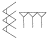
\includegraphics[scale=1]{22a.png}};
			\draw (0.5,1.05) node[above] {$\scriptstyle\times(60\times60)$};
			\draw (1.5,1.1) node[above] {$\scriptstyle\times60$};
			\draw (2.5,1.1) node[above] {$\scriptstyle\times1$};
		\end{tikzpicture}
		\vspace*{-10pt}
	\end{figure}
	Vậy 
\includegraphics[scale=0.9]{23}  $= 93$.
	\vskip 0.1cm
	Tiếp theo, chúng ta hãy thử viết số lớn hơn. Chúng ta hãy cùng viết số $3604$ bằng các chữ số Babylon nhé. Số $3604$ lớn hơn $60\times 60=3600$, nên ta cần biểu diễn số này từ hàng thứ ba tính từ hàng đơn vị. Ta chia số $3604$ cho $3600$ được thương là $1$ nên ta viết ký hiệu 
\includegraphics[scale=0.7]{15}  vào hàng $60\times60$
	\begin{figure}[H]
		\centering
		\vspace*{-5pt}
		\captionsetup{labelformat= empty, justification=centering}
		\begin{tikzpicture}[xscale=1.5,yscale=1.2,color=toancuabi]
			\draw (0,0) grid (3,1);
			\node[inner sep=0pt] (mouse) at (0.5,0.5){
\includegraphics[scale=1]{27a.png}};
			\draw (0.5,1.05) node[above] {$\scriptstyle\times(60\times60)$};
			\draw (1.5,1.1) node[above] {$\scriptstyle\times60$};
			\draw (2.5,1.1) node[above] {$\scriptstyle\times1$};
		\end{tikzpicture}
		\vspace*{-10pt}
	\end{figure}
	Số dư của phép chia là $4$ nhỏ hơn $60$ nên ta viết ký hiệu 
\includegraphics[scale=0.6]{15.1} vào hàng $60$, và $4$ ký hiệu 
\includegraphics[scale=0.7]{15} vào hàng đơn vị. 
	\begin{figure}[H]
		\centering
		\vspace*{-5pt}
		\captionsetup{labelformat= empty, justification=centering}
		\begin{tikzpicture}[xscale=1.5,yscale=1.2,color=toancuabi]
			\draw (0,0) grid (3,1);
			\node[inner sep=0pt] (mouse) at (0.5,0.5){
\includegraphics[scale=1]{27a.png}};
			\node[inner sep=0pt] (mouse) at (1.5,0.5){
\includegraphics[scale=1]{27b.png}};
			\node[inner sep=0pt] (mouse) at (2.5,0.5){
\includegraphics[scale=1]{27c.png}};
			\draw (0.5,1.05) node[above] {$\scriptstyle\times(60\times60)$};
			\draw (1.5,1.1) node[above] {$\scriptstyle\times60$};
			\draw (2.5,1.1) node[above] {$\scriptstyle\times1$};
		\end{tikzpicture}
		\vspace*{-10pt}
	\end{figure}
	Vậy, số $3604$ được người Babylon viết như sau:
	\begin{figure}[H]
		\centering
%		\vspace*{-5pt}
		\captionsetup{labelformat= empty, justification=centering}
		
\includegraphics[width=0.35\linewidth]{27}
		%	\caption{\textit{\color{toancuabi}Hình $1$.}}
		\vspace*{-10pt}
	\end{figure}
	Cách ghi số của người Ai Cập cổ, La Mã hay chúng ta ngày nay dùng cơ số $10$ còn cách ghi số của người Babylon sử dụng cơ số $60$. Do số $60$ chia hết cho nhiều số: $1,2,3,4,5,6, 10, 12, 15, 20,30$ và $60$, nên việc chia các đại lượng được thực hiện dễ dàng hơn, ít phải dùng đến các phân số. Việc sử dụng đơn vị thời gian: $1$ phút $= 60$ giây, $1$ giờ $= 60$ phút ngày nay là một ảnh hưởng của người Babylon đấy.
	\vskip 0.1cm
	\textbf{\color{toancuabi}Số Maya}
	\vskip 0.1cm
	\begin{figure}[H]
		\centering
		\vspace*{-10pt}
		\captionsetup{labelformat= empty, justification=centering}
		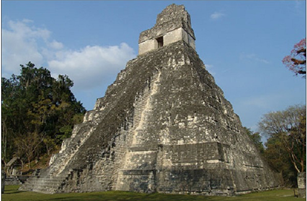
\includegraphics[width=1\linewidth]{28}
		\caption{\textit{\color{toancuabi}Kim tự tháp Tikal của người Maya.}}
		\vspace*{-10pt}
	\end{figure}
	Người Maya  được cho là đã xuất hiện từ rất xa xưa. Họ đã xây dựng hệ thống lịch chính xác và toán học của họ là đại diện tiêu biểu cho toán học của dân cư ở châu Mỹ thời cổ đại.
	\vskip 0.1cm
	Nói về cách ghi số,  người Maya dùng hệ cơ số $20$, gồm $3$ ký hiệu:  
\includegraphics[scale=0.7]{29},  
\includegraphics[scale=0.7]{30}, \includegraphics[scale=0.7]{31}  ứng với $0,1, 5$ và biểu diễn số theo chiều dọc. Chữ số ở hàng cao hơn được viết phía trên, chữ số ở hàng thấp hơn được viết phía dưới. Điều này tương tự chúng ta viết số ngày nay: ta đặt số ở hàng cao hơn bên trái còn số ở hàng thấp hơn bên phải. 
	\begin{table}[H]
		\vspace*{-5pt}
		\centering
		\setlength{\tabcolsep}{4.5pt}
		\renewcommand{\arraystretch}{1.3}
		\begin{tabular}{|l|l|}
			\hline
			$10^3 = 10\!\times\! 10 \!\times\! 10 =1000$& hàng nghìn\\
			\hline
			$10^2 = 10\!\times\! 10 =100$& hàng trăm\\
			\hline
			$10^1 = 10$& hàng chục\\
			\hline
			$10^0 = 1$& hàng đơn vị\\
			\hline
		\end{tabular}
%		\vspace*{-5pt}
	\end{table}
	Do sử dụng hệ cơ số $20$,  số Maya được biểu diễn trong phần bên phải của bảng trong Hình $3$ chính là số  $1\times 8000+ 0\times 400+ 10\times20+ 7\times1= 8207$. Bởi vì, ta  thấy  \includegraphics[scale=0.3]{33},  \includegraphics[scale=0.3]{34},  \includegraphics[scale=0.3]{35}, \includegraphics[scale=0.3]{36}  ứng với $1, 0, 10, 7$  lần lượt ở các hàng $8000$, $400$, $20$ và đơn vị. Chú ý rằng, trong một hàng, chữ số có giá trị cao hơn lại được viết phía dưới chữ số có giá trị lớn hơn chẳng hạn  \includegraphics[scale=0.3]{36}:  hai ký hiệu \includegraphics[scale=0.7]{37} (số $1$) được viết bên trên ký hiệu \includegraphics[scale=0.7]{38} (số $5$). Ký hiệu \includegraphics[scale=0.3]{34} để biểu diễn $0$ ở một hàng giống như ta viết $101$ và giúp ta phân biệt số $101$ với số $11$. Điều này cũng tương tự như cách ghi số Babylon. 
	\begin{table}[H]
		\vspace*{-5pt}
		\centering
		\captionsetup{labelformat= empty, justification=centering}
		\setlength{\tabcolsep}{21pt}
		\renewcommand{\arraystretch}{1.25}
		\begin{tabular}{|l|c|}
			\hline
			$20\times 20\times 20 =8000$  & \includegraphics[scale=0.3]{33} \\
			\hline
			$20\times 20 =400$     & \includegraphics[scale=0.3]{34} \\
			\hline
			$20$ & \includegraphics[scale=0.3]{35}\\
			\hline
			$1$& \includegraphics[scale=0.3]{36.png}\\
			\hline
		\end{tabular}
		\caption{\small\textit{\color{toancuabi}Hình $3$.}}
		\vspace*{-10pt}
	\end{table}
	Người ta cho rằng hệ cơ số $10$ được dùng phổ biến vì con người có $10$ ngón tay, còn người Maya vốn không đi giày nên họ đếm bằng cả các ngón chân nữa. Họ dùng hệ cơ số $20$ là vì thế!
	\begin{figure}[H]
		\centering
		\vspace*{-5pt}
		\captionsetup{labelformat= empty, justification=centering}
		\includegraphics[width=1\linewidth]{20.12-pi.4-2}
		\vspace*{-12pt}
	\end{figure}
	\vskip 0.1cm
	\textbf{\color{toancuabi}Số Trung Hoa cổ}
	\vskip 0.1cm
	Trung Hoa cổ đại cũng là một trong những nền văn minh cổ lớn của thế giới. Khoảng $3500$ năm trước, người Trung Hoa khắc lên những mảnh mai rùa những ký hiệu khác nhau thể hiện số và chữ. Một số trong đó như~sau:
	\begin{figure}[H]
		\centering
		\vspace*{5pt}
		\captionsetup{labelformat= empty, justification=centering}
		\includegraphics[height=0.8\linewidth]{china1}\quad
		\includegraphics[height=0.8\linewidth]{41}
		\caption{\textit{\color{toancuabi}Một số ký hiệu viết trên một mảnh mai rùa.}}
		\vspace*{-10pt}
	\end{figure}
	Cách ghi số Trung Hoa cổ tương tự như cách ghi số La Mã: Các chữ số giá trị lớn được đặt bên trái các chữ số có  giá trị nhỏ hơn, số được biểu diễn có giá trị bằng tổng các chữ số trong biểu diễn của nó. Ví dụ \includegraphics[scale=0.25]{china5} biểu diễn số $500 + 30 + 5 = 535$. Những biểu tượng khắc trên những mảnh mai rùa phát triển theo thời gian và hình thành nên chữ viết của người Trung Hoa ngày nay. 
	\begin{figure}[H]
		\centering
		\vspace*{-5pt}
		\captionsetup{labelformat= empty, justification=centering}
		\includegraphics[width=0.9\linewidth]{20.12-pi.3}
		\vspace*{-10pt}
	\end{figure}
	Các bạn có thấy rằng cách biểu diễn số của người Ai Cập, La Mã và Trung Hoa cổ có điểm tương đồng? Người ta nói đó là những hệ thống số ``\textit{đơn phân}". Mỗi ký hiệu thể hiện một giá trị không thay đổi cho dù nó đứng ở vị trí nào. Mỗi số viết ra biểu diễn một đại lượng được xác định bằng cách  cộng (hay trừ như ở số La Mã) những giá trị tương ứng với các ký hiệu được sử dụng trong đó. Số mà chúng ta dùng ngày nay là một hệ thống số ``\textit{sắp theo hàng}" vì các ký hiệu có giá trị phụ thuộc vào hàng mà nó được xếp vào. Ở hàng chục, số $1$ có nghĩa là một chục, nhưng số $1$ ở hàng đơn vị có nghĩa là $1$ đơn vị. Trong khi đó, số của người Babylon và Maya là một dạng hỗn hợp vừa được ``\textit{sắp theo hàng}" vừa cần cộng những ký hiệu trong mỗi hàng để biết giá trị của số được biểu diễn.
	\vskip 0.1cm
	Vậy là qua bài viết này chúng ta đã biết những cách ghi số  từ thời xa xưa con người ở những nơi khác nhau trên Trái Đất. Những đại lượng phức tạp hơn như phân số chẳng hạn cũng đã được người cổ đại viết ra và sử dụng. Chúng ta sẽ tìm hiểu thêm về những thành tựu toán học của loài người ở những thời kỳ trước đây trong những số báo sắp tới nhé. 
	\vskip 0.1cm
	\textbf{\color{toancuabi}Bài tập} $\pmb{1.}$
	Em viết các số sau theo cách viết số ngày nay
	\vskip 0.1cm
	$\bullet$ \includegraphics[scale=0.5]{babylon1}
	\vskip 0.1cm
	$\bullet$ \includegraphics[scale=0.42]{babylon2}
	\vskip 0.1cm
	$\bullet$ \includegraphics[scale=0.42]{maya1}
	\vskip 0.1cm
	$\bullet$ \includegraphics[scale=0.42]{maya2}
	\vskip 0.1cm
	$\bullet$ \includegraphics[scale=0.5]{china2}
	\vskip 0.1cm
	$\bullet$ \includegraphics[scale=0.5]{china4}
	\vskip 0.1cm
	\textbf{\color{toancuabi}Bài tập} $\pmb{2.}$ Em hãy viết số $2022$ theo cách ghi số Babylon, Maya và Trung Hoa cổ.
	\vskip 0.1cm
	\textbf{\color{toancuabi}Tài liệu, nguồn tham khảo}
	\vskip 0.1cm
	[$1$] R. L. Cooke, History of math, Wiley, $2013$.
	\vskip 0.1cm
	[$2$] \url{https://www.britannica.com/}
	\vskip 0.1cm
	[$3$] \url{https://www.penn.museum/}
	\vskip 0.1cm
	[$4$] \url{https://www.cemc.uwaterloo.ca}
\end{multicols}
\newpage
\graphicspath{{../toancuabi/pic/}}
\begingroup
\AddToShipoutPicture*{\put(150,680){\includegraphics[scale=1]{../tieude.pdf}}} 
\centering
\endgroup
\vspace*{25pt}

\begin{multicols}{2}
	Trong giờ nghỉ trưa, thám tử Xuân Phong vẫn đang ngồi miệt mài đọc các tài liệu điều tra phá án, thì bỗng ``choang", một tiếng vỡ chói tai vang lên từ phía cửa sổ. Ngẩng lên, Xuân Phong nhìn thấy $4$ cậu thiếu niên chạy thục mạng về phía cuối phố. Chắc hẳn lại là một trò nghịch tinh quái nào đó rồi.
	\vskip 0.15cm 
	Xuân Phong nhờ phía cảnh sát đưa $4$ cậu thiếu niên nghịch ngợm này vào trụ sở để thẩm vấn. Bốn cậu lần lượt tên là An, Vinh, Sinh và Du. An tuyên bố ``Vinh là người làm vỡ kính", Vinh lại khẳng định ``Sinh là người có lỗi",  Sinh thì quả quyết ``Vinh là người nói dối đấy", còn Du thề rằng ``Cháu không làm điều này". 
	Sau một hồi nói chuyện, Xuân Phong mới biết rằng chỉ có duy nhất một cậu thiếu niên trong số họ là nói thật. Vậy ai là người làm vỡ kính phòng làm việc của thám tử Xuân Phong nhỉ?
	\begin{figure}[H]
		\vspace*{-5pt}
		\centering
		\captionsetup{labelformat= empty, justification=centering}
		\includegraphics[width= 1\linewidth]{xp}
		\vspace*{-12pt}
	\end{figure}
\end{multicols}
\vspace*{-10pt}
\rule{1\linewidth}{0.1pt}
\begingroup
\AddToShipoutPicture*{\put(112,380){\includegraphics[scale=1]{../tieude11.pdf}}} 
\centering
\endgroup
\vspace*{46pt}

\begin{multicols}{2}
	$\pmb{1.}$ Có $30$ bạn học sinh tham gia một cuộc thi hùng biện bằng tiếng Anh. Các bạn lần lượt chọn các câu hỏi và trả lời theo thứ tự xếp hàng. Bạn thứ nhất được $80$ điểm, bạn thứ hai được $60$ điểm, bạn thứ ba có số điểm bằng trung bình cộng của bạn thứ nhất và bạn thứ hai, bạn thứ tư có số điểm bằng trung bình cộng của ba bạn đầu tiên. Nói chung, kể từ bạn thứ ba trở đi thì cứ mỗi một bạn học sinh tiếp theo luôn có số điểm bằng trung bình cộng số điểm của các bạn đã thi trước đó. 
	\begin{figure}[H]
		\centering
		\vspace*{-5pt}
		\captionsetup{labelformat= empty, justification=centering}
		\includegraphics[width=0.92\linewidth]{bai1}
%		\vspace*{-5pt}
	\end{figure}
	Hỏi bạn cuối cùng, tức bạn có số thứ tự $30$, đạt được bao nhiêu điểm trong cuộc thi? 
	\vskip 0.1cm
	$\pmb{2.}$ Vào một ngày hè, ba bạn Yến, Vinh và Công đến hiệu kem và mỗi bạn đều lấy đủ $3$ vị: trái cây, vani và sô--cô--la (mỗi vị một cốc). Sau khi ăn xong, vì $3$ cốc cho một người là chưa đủ, nên Yến lấy thêm một cốc kem trái cây, Vinh lấy thêm một cốc kem vani và Công lấy thêm một cốc kem sô--cô--la. 
	\begin{figure}[H]
		\centering
		\vspace*{-5pt}
		\captionsetup{labelformat= empty, justification=centering}
		\includegraphics[width=0.9\linewidth]{bai2}
		\vspace*{-5pt}
	\end{figure}
	Lúc ra quầy thanh toán, Yến phải trả $70$ nghìn, Vinh phải trả $80$ nghìn còn Công phải trả $90$ nghìn. Hỏi mỗi vị kem có giá bao nhiêu tiền một cốc?
	\vskip 0.1cm
	$\pmb{3.}$ Ba chú khỉ con dễ thương có tên là Bibi, Bobo, và Bubu được diện áo và giày thật đẹp để quay video đăng YouTube. Các chú được mặc $3$ chiếc áo có các màu khác nhau là đỏ, xanh lá cây và xanh lơ. Giày của ba chú cũng có $3$ màu như thế, mỗi chú mang một đôi khác màu với chú khác. Bibi thì diện áo và giày có cùng màu. Bobo lại không thích màu đỏ, nên cả giày và áo đều không phải đỏ. Bubu thì mang giày xanh lá cây, còn áo lại có màu khác. Vậy các chú khỉ đã mặc áo và đi giày có màu như thế nào nhỉ?
	\begin{figure}[H]
		\centering
		\vspace*{-5pt}
		\captionsetup{labelformat= empty, justification=centering}
		\includegraphics[width=1\linewidth]{bai3}
		\vspace*{-15pt}
	\end{figure}
	$\pmb{4.}$ Để chuẩn bị cho cuộc đua xe đạp sắp diễn ra, sáng sớm Gấu con đã mang xe ra tập luyện. Lúc đi tốc độ của Gấu con là $15$ dặm/giờ. Do đường khá đông nên chiều trở về dù vẫn đi trên con đường đó nhưng Gấu con chỉ di chuyển với tốc độ $10$ dặm/giờ. Hỏi trên cả quãng đường lúc đi và về vận tốc trung bình của Gấu con là bao nhiêu?
	\begin{figure}[H]
		\centering
		\vspace*{5pt}
		\captionsetup{labelformat= empty, justification=centering}
		\includegraphics[width=1\linewidth]{bai5}
		\vspace*{-15pt}
	\end{figure}
	$\pmb{5.}$ Trên bàn có một đống đá cuội gồm $1001$ viên. Người ta lấy ra một viên đá và chia đống đá ra thành hai đống mới. Bây giờ, trong mỗi một đống đá có ít nhất $3$ viên, người ta lại lấy ra một viên đá và lại chia đống đó ra thành hai đống mới, và cứ tiếp tục như vậy. Hỏi có thể sau một số lần lấy đi các viên đá, trên bàn chỉ còn toàn các đống đá mà mỗi đống có đúng $3$ viên được hay không?
	\begin{figure}[H]
		\centering
		\vspace*{-5pt}
		\captionsetup{labelformat= empty, justification=centering}
		\includegraphics[width=1\linewidth]{bai4}
		\vspace*{-15pt}
	\end{figure}
	$\pmb{6.}$ Thạch Sanh chuẩn bị lên đường tiêu diệt Mãng xà -- con chằn tinh có tận $3$ cái đầu và $3$ cái đuôi gớm ghiếc. Ngài Thần Miếu đưa cho chàng một bảo bối và dặn dò: ``Đây là chiếc gươm thần thiêng liêng. Bằng một nhát gươm, con có thể chém đứt được một cái đầu, hoặc là hai cái đầu, hoặc là một cái đuôi, hoặc là hai cái đuôi của con Mãng xà. Nhưng con nên nhớ, nếu con chỉ chém đứt một cái đầu, thì một cái đầu khác của nó sẽ mọc lên, nếu chỉ chém đứt một cái đuôi, thì hai cái đuôi khác lại mọc ra, nếu chém đứt hai cái đuôi thì một cái đầu khác lại mọc ra, còn nếu con chém đứt được hai cái đầu thì không có gì mọc ra thêm nữa". Vậy Thạch Sanh có thể chém đứt tất cả đầu và đuôi của con Mãng xà sau bao nhiêu nhát gươm?
	\begin{figure}[H]
		\centering
		\vspace*{-5pt}
		\captionsetup{labelformat= empty, justification=centering}
		\includegraphics[width=1\linewidth]{bai6}
		\vspace*{-5pt}
	\end{figure}
\end{multicols}
\newpage
\begingroup
\AddToShipoutPicture*{\put(112,640){\includegraphics[scale=1]{../tieude2.pdf}}} 
\centering
\endgroup
\graphicspath{{../toancuabi/pic/}}
\vspace*{65pt}

\begin{multicols}{2}
	$\pmb{1.}$ Trong một kỳ nghỉ hè, Tâm và Bảo cùng đi du lịch trên một chuyến tàu hỏa. Hai toa mà họ ngồi là các toa liền kề nhau. Toa tàu của Tâm là toa thứ $5$ tính từ đầu tàu, còn toa  của Bảo lại là toa thứ $7$ tính từ đuôi tàu. Hỏi đoàn tàu của hai bạn hôm đó có bao nhiêu toa?
	\begin{figure}[H]
		\vspace*{-5pt}
		\centering
		\captionsetup{labelformat= empty, justification=centering}
		\includegraphics[width= 1\linewidth]{b1}
		\vspace*{-15pt}
	\end{figure}
	\textit{Lời giải.} Tùy thuộc vào việc Tâm ngồi gần đầu tàu hơn Bảo hay Bảo ngồi gần đầu tàu hơn Tâm.
	\vskip 0.1cm
	Nếu Tâm ngồi gần hơn, rõ ràng số toa là $5+7=12$.
	\vskip 0.1cm
	Tuy nhiên, nếu Bảo ngồi gần đầu tàu hơn, thì số toa sẽ là $5+7-2=10$ (toa).
	\vskip 0.1cm
	Ở đây $2$ là hai toa của Tâm và Bảo.
	\vskip 0.1cm
	$\pmb{2.}$	Có ba người bạn muốn đi ca nô vượt qua một con sông, chở theo một cái tủ lạnh. Chiếc ca nô chỉ đủ chỗ cho $2$ người và tủ lạnh, hoặc chỉ cho $3$ người. Nhưng rắc rối ở chỗ là cái tủ lạnh quá nặng, nên phải có cả sức $3$ người mới đủ để khiêng nó lên ca nô hoặc đẩy xuống khỏi ca nô. Hỏi họ có thể qua được sông hay không?
	\begin{figure}[H]
		\vspace*{-10pt}
		\centering
		\captionsetup{labelformat= empty, justification=centering}
		\includegraphics[width= 1\linewidth]{b2}
		\vspace*{-15pt}
	\end{figure}
	\textit{Lời giải.} Lần đầu tiên ta cho hai bạn đi cùng chiếc tủ lạnh sang sông, một bạn sang bên kia, còn một bạn quay lại cùng chiếc tủ lạnh. Sau khi đón bạn còn lại ở bên bờ bên này, hai bạn cùng đi lần cuối cùng chiếc tủ lạnh sang nốt bên bờ bên kia, ở đó có một bạn đợi sẵn để chuyển tủ lạnh khỏi ca nô xuống bờ.
	\vskip 0.1cm
	$\pmb{3.}$ Trong một vương quốc nọ các thần dân chia thành $2$ nhóm người: một nhóm Thật thà gồm toàn những người nói thật, và nhóm kia là Dối trá gồm toàn những người chỉ nói dối. Trong một buổi tối nọ, có $10$ người lần lượt bước vào một ngôi nhà, mỗi người trong số họ (trừ người cuối cùng) viết trên một mảnh giấy đặc biệt để thông báo người sẽ vào tiếp theo anh ta là Thật thà hay Dối trá. Nếu như tin vào những gì viết trên $9$ mảnh giấy đó, thì toàn là người Dối trá đã bước vào nhà. Hỏi trên thực tế có tất cả bao nhiêu người Dối trá đã tới ngôi nhà đó.	
	\begin{figure}[H]
		\vspace*{-5pt}
		\centering
		\captionsetup{labelformat= empty, justification=centering}
		\includegraphics[width= 1\linewidth]{b3}
		\vspace*{-15pt}
	\end{figure}
	\textit{Lời giải.} Mỗi một người Thật thà (trừ người đầu tiên) bước vào nhà đều phải có một người Dối trá đi trước anh ta, còn mỗi người Dối trá thì lại phải có một người Thật thà đi đằng trước. Suy ra, trong cả hai trường hợp người đầu tiên là Thật thà hay Dối trá, có tất cả $5$ người Thật thà và $5$ người Dối trá đã bước vào nhà đó.
	\vskip 0.1cm
	$\pmb{4.}$ Hai chiếc máy bơm cùng nhau bơm đầy nước cho một bể bơi trong vòng $2$ giờ. Hỏi mỗi chiếc máy bơm sẽ bơm đầy bể trong bao nhiêu lâu, biết rằng thời gian bơm đầy của hai máy bơm tính theo giờ là các số nguyên khác nhau.
	\begin{figure}[H]
		\vspace*{-5pt}
		\centering
		\captionsetup{labelformat= empty, justification=centering}
		\includegraphics[width= 0.9\linewidth]{b4}
		\vspace*{-10pt}
	\end{figure}
	\textit{Lời giải.} 	Giả sử một máy bơm đầy bể trong $a$ (giờ) còn máy kia trong $b$ (giờ). Ta có $a,b$ là các số nguyên khác nhau. Trong $1$ giờ, máy thứ nhất bơm được $\dfrac{1}{a}$ phần bể, còn máy kia bơm được $\dfrac{1}{b}$ phần bể. Theo giả thiết $\dfrac{1}{a}+\dfrac{1}{b}= \dfrac{1}{2}$.
	\vskip 0.1cm
	Rõ ràng $a,b$ phải lớn hơn $2$. Không mất tính tổng quát, giả sử $2<a<b$. 
	\vskip 0.1cm
	Nếu $a = 3$ thì ta có $b = 6$.
	\vskip 0.1cm
	Nếu $a \ge 4$, suy ra $b \ge 5$, và $\dfrac{1}{a} + \dfrac{1}{b} < \dfrac{1}{4} + \dfrac{1}{4} = \dfrac{1}{2}$, do đó ta loại những trường hợp này.
	\vskip 0.1cm
	Vậy một máy bơm đầy bể trong $3$ giờ và máy còn lại bơm đầy bể trong $6$ giờ.
	\vskip 0.1cm
 	$\pmb{5.}$ Trên một hòn đảo nọ có các thổ dân sinh sống, một số người thì luôn nói thật, còn những người còn lại thì luôn nói dối. Một lần nọ, ba thổ dân là anh Tit, anh Te và anh Tu gặp nhau. Một người trong số họ nói ``Tit và Te -- cả hai đều là những  người nói dối'', một người khác nói ``Tit và Tu -- cả hai đều là những người nói dối" (tuy nhiên không rõ chính xác ai nói những câu này). Hỏi có bao nhiêu người nói dối trong số $3$ người này?
	\begin{figure}[H]
		\vspace*{-5pt}
		\centering
		\captionsetup{labelformat= empty, justification=centering}
		\includegraphics[width= 1\linewidth]{b5}
		\vspace*{-15pt}
	\end{figure}
	\textit{Lời giải.} Có tất cả $2$ người nói dối trong số họ. Thật vậy, nếu trong số $3$ người trên có không quá $1$ người nói dối, thì trong số hai câu nói trên, phải có ít nhất một câu là thật (do hai người khác nhau nói ra). Nhưng theo bất kỳ câu nào, thì số người nói dối trong họ phải ít nhất là $2$. Suy ra vô lý.
	\vskip 0.1cm
	Nếu cả $3$ người cùng nói dối, thì cả $2$ câu đều là thật, mà lại do các người nói dối phát biểu. Điều này cũng không thể.
	\vskip 0.1cm
	Vì vậy số người nói dối phải đúng bằng $2$.
	\vskip 0.1cm
	Ta còn phải đưa ra ví dụ về tình huống có thể xảy ra. Ví dụ như anh Tit là người nói thật, còn hai câu trên đều do hai anh nói dối phát ngôn.
	\vskip 0.1cm
	$\pmb{6.}$ Có $10$ cái hộp bút, mỗi hộp đựng một số chiếc bút chì màu, không có hộp nào là rỗng. Biết rằng số bút chì ở hai hộp bất kỳ là khác nhau, hơn nữa những chiếc bút chì trong mỗi hộp đều có màu khác nhau, em hãy chỉ ra là có thể nhặt ra từ mỗi chiếc hộp một chiếc bút để nhận được $10$ chiếc bút chì có màu hoàn toàn khác nhau. 
	\begin{figure}[H]
		\vspace*{-5pt}
		\centering
		\captionsetup{labelformat= empty, justification=centering}
		\includegraphics[width= 1\linewidth]{b6}
		\vspace*{-15pt}
	\end{figure}
	\textit{Lời giải.} Ta sắp xếp các hộp bút theo thứ tự tăng dần về số bút chì trong hộp. Vậy hộp thứ nhất có ít nhất $1$ chiếc, hộp thứ hai có ít nhất $2$ chiếc, vv.. và hộp thứ $10$ có ít  nhất $10$ chiếc bút.
	\vskip 0.1cm
	Trong hộp thứ nhất ta lấy $1$ chiếc bút, gọi màu của nó là $A$. Vì trong hộp thứ $2$ có ít nhất hai bút khác màu, nên ít nhất phải có một chiếc bút trong hộp này, khác màu với $A$. Ta gọi chiếc bút này có màu $B$. Trong hộp $3$ có ít nhất $3$ chiếc bút khác màu nhau, nên phải có ít nhất một chiếc bút khác màu với $A$ và $B$. Ta lấy ra chiếc bút đó. Cứ làm liên tiếp như vậy ta có thể lấy ra ở mỗi hộp một chiếc bút theo như yêu cầu đề bài.
\end{multicols}
\newpage
\begingroup
\thispagestyle{toancuabinone}
\blfootnote{$^1$\color{toancuabi}Trường THCS Archimedes, Hà Nội.}
\AddToShipoutPicture*{\put(60,733){\includegraphics[width=17.2cm]{../mathc.pdf}}}
%\AddToShipoutPicture*{\put(-2,733){\includegraphics[width=17.2cm]{../mathl.pdf}}} 
\AddToShipoutPicture*{\put(192,675){\includegraphics[scale=1]{../tieude3.pdf}}} 
\centering
\endgroup
\graphicspath{{../toancuabi/pic/}}
\vspace*{35pt}

\begin{multicols}{2}
	\PIbox{\textbf{\color{toancuabi}Problem} $\pmb{1.}$ How many ways are there to go from $A$ to $B$ in the directions indicated by the pink arrows?}
	\begin{center}
		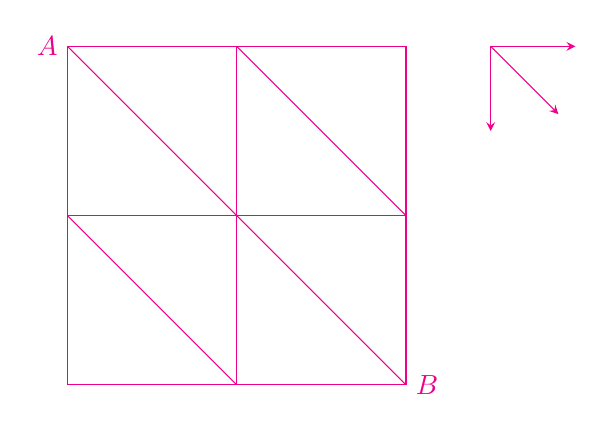
\begin{tikzpicture}[color=toancuabi, xscale=2.15, yscale=2.15]
			\draw (0,0) grid (2,2);
			\draw (0,2) node[left] {$A$};
			\draw (2,0) node[right] {$B$};
			\draw [-stealth] (2.5,2) --(3,2);
			\draw [-stealth] (2.5,2) --(2.9,1.6);
			\draw [-stealth] (2.5,2) --(2.5,1.5);
			\draw (0,1) --(1,0) (0,2) -- (2,0) (1,2) -- (2,1);
		\end{tikzpicture}
	\end{center}
	\PIbox{\textbf{\color{toancuabi}Rule of Sum:} Suppose that we have to do two independent jobs $A$ and $B$, and that there are $m$ ways to do job $A$ and $n$ ways to do job $B$. We cannot do both jobs at the same time, therefore there are $(m + n)$ ways to do one of the two jobs (either job $A$ or job $B$).}
	\vskip 0.1cm
	\textit{Solution:} In the picture below, the number at each node indicates how many ways we can go from $A$ to that node. 
	\begin{center}
		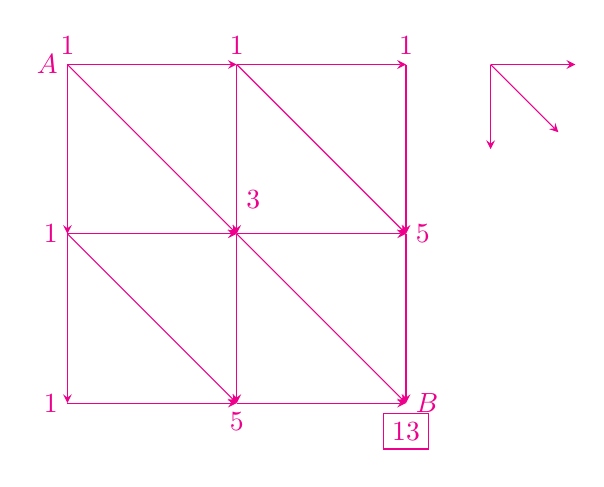
\begin{tikzpicture}[color=toancuabi, xscale=2.15, yscale=2.15]
			\draw (0,2) node[left] {$A$};
			\draw (0,2) node[above] {$1$};
			\draw (1,2) node[above] {$1$};
			\draw (2,2) node[above] {$1$};
			\draw (2,1) node[right] {$5$};
			\draw (0,1) node[left] {$1$};
			\draw (1,1.2) node[right] {$3$};
			\draw (2,0) node[below] {$\boxed{13}$};
			\draw (0,0) node[left] {$1$};
			\draw (1,0) node[below] {$5$};
			\draw (2,0) node[right] {$B$};
			\draw [-stealth] (2.5,2) --(3,2);
			\draw [-stealth] (2.5,2) --(2.9,1.6);
			\draw [-stealth] (2.5,2) --(2.5,1.5);
			\draw[-stealth] (0,1) --(1,0); 
			\draw[-stealth] (0,2) -- (1,1);
			\draw[-stealth] (1,1) -- (2,0);
			\draw[-stealth] (1,2) -- (2,1);
			\draw[-stealth]	(0,2) -- (0,1);
			\draw[-stealth]	(0,1) -- (0,0);
			\draw[-stealth]	(0,0) -- (1,0);
			\draw[-stealth]	(1,0) -- (2,0);
			\draw[-stealth]	(2,2) -- (2,1);
			\draw[-stealth]	(2,1) -- (2,0);
			\draw[-stealth]	(0,2) -- (1,2);
			\draw[-stealth] (1,2) -- (2,2);
			\draw[-stealth] (0,1) -- (1,1);
			\draw[-stealth]	(1,1) -- (2,1);
			\draw[-stealth]	(1,2) -- (1,1);
			\draw[-stealth] (1,1) -- (1,0);
		\end{tikzpicture}
	\end{center}
	To go from $A$ to $B$, we must pass through one of the three points which lie directly in front of it in the directions of the arrows. These are the points indicated by the numbers $5$, $3$, $5$. Thus, the number of ways to go from $A$ to $B$ is given by
	\begin{align*}
		\text{Rule of Sum: } 5+3+5=13.
	\end{align*}
%	\textit{Answer:} $13$
%	\vskip 0.1cm
	\PIbox{\textbf{\color{toancuabi}Problem} $\pmb{2.}$ How many ways are there to go from $A$ to $B$ in the directions indicated by the given blue arrows?}
	\begin{center}
		\begin{tikzpicture}[color=toancuabi,,scale=1.1]
			\draw (0,0) rectangle (3,3);
			\draw (0,0) node[left] {$A$};
			\draw (4,4) node[right] {$B$};
			\draw[dashed] (0,0) -- (1,1) (1,1) --(4,1) (1,1) --(1,4);
			\draw (1,4) -- (4,4) (4,4) -- (3,3) (4,4) -- (4,1) (4,1) -- (3,0) (1,4) -- (0,3); 
			\draw [quantoan,-stealth] (5,1) --(5,2);
			\draw [quantoan,-stealth] (5,1) --(5.8,1.8);
			\draw [quantoan,-stealth] (5,1) --(6,1);
		\end{tikzpicture}
	\end{center}
	\textit{Solution:} 
	Using the same argument as in Problem $1$, we have:
	\begin{align*}
		\text{Rule of Sum: } 2+2+2=6.
	\end{align*}
	\begin{center}
		\begin{tikzpicture}[color=toancuabi,scale=1.1]
			\draw (0,0) rectangle (3,3);
			\draw (0,0) node[left] {$A$};
			\draw (4,4) node[above] {$B$};
			
			\draw (1,1) node[left] {$1$};
			\draw (4,4) node[right] {$6$};
			\draw (3,3) node[above] {$2$};
			\draw (3.1,0) node[right] {$1$};
			\draw (1,4) node[above] {$2$};
			\draw (4,1) node[right] {$2$};
			\draw[dashed] (0,0) -- (1,1) (1,1) --(4,1) (1,1) --(1,4);
			\draw (1,4) -- (4,4) (4,4) -- (3,3) (4,4) -- (4,1) (4,1) -- (3,0) (1,4) -- (0,3); 
			\draw [quantoan,-stealth] (5,1) --(5,2);
			\draw [quantoan,-stealth] (5,1) --(5.8,1.8);
			\draw [quantoan,-stealth] (5,1) --(6,1);
		\end{tikzpicture}
	\end{center}
%	\textit{Answer:} $6$
%	\vskip 0.1cm
	\PIbox{\textbf{\color{toancuabi}Problem} $\pmb{3.}$ How many different moves can a knight on an $8\times8$ chessboard make?}
	\vskip 0.05cm
	\textit{Problem analysis:} A knight can go from any of the $64$ squares on a chessboard.
	\vskip 0.1cm
	$\circ$ If the knight stands on a corner square, it has two possible moves.
	\vskip 0.1cm
	$\circ$ If the knigh stands on a side square next to a corner square, it has three possible moves.
	\vskip 0.1cm
	$\circ$ If the knight stands on another side square, it has four possible moves, and so on.
	\vskip 0.1cm
	$\circ$ The maximum number of moves for a knight is eight when it stands on a square where it can move in all possible directions.
	\vskip 0.1cm
	The table below shows the number of moves a knight can make from each square on the board:
	\begin{center}
		\def\myNotes{{{2,3,4,4,4,4,3,2},{3,4,6,6,6,6,4,3},{4,6,8,8,8,8,6,4},{4,6,8,8,8,8,6,4},{4,6,8,8,8,8,6,4},{4,6,8,8,8,8,6,4},{3,4,6,6,6,6,4,3},{2,3,4,4,4,4,3,2}}} 
		\begin{tikzpicture}[scale=0.88,color=cackithi]
			\foreach \x  in {1,2,...,8}
			\foreach \y in {1,2,...,8}
			{	
				\draw (\x,\y*-1) +(-.5,-.5) rectangle ++(.5,.5);
				\begin{scope}[shift={(\x,\y*-1)}]
					\pgfmathtruncatemacro{\r}{\myNotes[\y-1][\x-1]}
					\coordinate (C) at (0,0,0);
					\node (C) {$\r$};
				\end{scope}
			}
		\end{tikzpicture}
	\end{center}
	Thus, the total number of moves that the knight can make on an $8\times8$ chessboard is: 
	\begin{align*}
		&\text{Rule of Sum: }\\
		&2\times4 \!+\! 3\!\times\!8 \!+\! 4\!\times\!20 \!+\! 6\!\times\!16 \!+\! 8\!\times\!16 \!=\! 336.
	\end{align*}
%	\textit{Answer:} $336$.
%	\vskip 0.1cm
	\PIbox{\textbf{\color{toancuabi}Exercise} $\pmb{1.}$ How many ways are there to go from $A$ to $B$ in the directions indicated by the pink arrows?}
	\begin{center}
		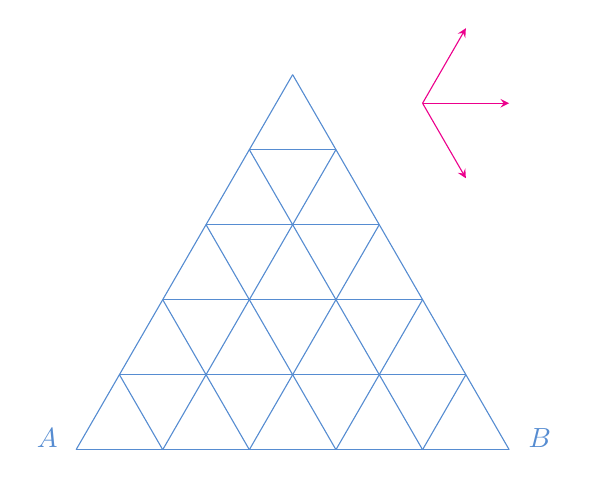
\begin{tikzpicture}[color=cackithi,scale=1.1]
			\draw  (0.,0.)-- (5.,0.);
			\draw  (5.,0.)-- (2.5,4.330127018922194);
			\draw  (2.5,4.330127018922194)-- (0.,0.);
			\draw  (2.,3.464101615137755)-- (3.,3.4641016151377553);
			\draw  (1.5,2.598076211353316)-- (3.5,2.5980762113533165);
			\draw  (1.,1.7320508075688774)-- (4.,1.732050807568878);
			\draw  (0.5,0.8660254037844387)-- (4.5,0.8660254037844392);
			\draw  (1.,0.)-- (3.,3.4641016151377553);
			\draw  (3.5,2.5980762113533165)-- (2.,0.);
			\draw  (4.,1.732050807568878)-- (3.,0.);
			\draw  (4.5,0.8660254037844392)-- (4.,0.);
			\draw  (4.,0.)-- (2.,3.464101615137755);
			\draw  (1.5,2.598076211353316)-- (3.,0.);
			\draw  (2.,0.)-- (1.,1.7320508075688774);
			\draw[-stealth,toancuabi]  (4.,4.)-- (4.5,4.86602540378444);
			\draw[-stealth,toancuabi]  (4.,4.)-- (5.,4.);
			\draw[-stealth,toancuabi]  (4.,4.)-- (4.5,3.133974596215561);
			\draw  (1.,0.)-- (0.5,0.8660254037844387);
		

			\draw (-0.3328996275042767,0.139482532970907) node {$A$};

			\draw (5.354808013691732,0.139482532970907) node {$B$};
		
		\end{tikzpicture}
	\end{center}
	\PIbox{\textbf{\color{toancuabi}Exercise} $\pmb{2.}$ A bug walks along the lines on the grid in the directions indicated by the blue arrows. How many ways can it get from $A$ to $B$?}
	\begin{center}
		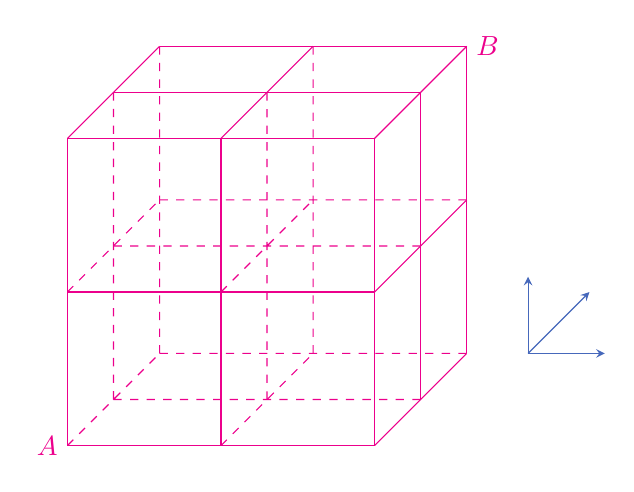
\begin{tikzpicture}[xscale=1.95, yscale=1.95, toancuabi]
			\draw (0,0) grid (2,2);
			\draw[dashed] (0.6,0.6) -- (0.6, 2.6)  (2.6,0.6) -- (0.6,0.6) (0.3,0.3) -- (0.3, 2.3)  (2.3,0.3) -- (0.3,0.3) (0,0) -- (0.6,0.6);
			\draw (0.6,2.6) -- (2.6,2.6) (2.6,2.6) -- (2.6,0.6) (0.3,2.3) -- (2.3,2.3) (2.3,2.3) -- (2.3,0.3);
			\draw (0,2) -- (0.6, 2.6) (1,2) -- (1.6, 2.6) (2,2) -- (2.6,2.6) (2,1) --(2.6,1.6) (2,0) -- (2.6,0.6);
			\draw[dashed] (1,0) -- (1.6, 0.6) (1.6, 0.6) -- (1.6,2.6) (0,1) -- (0.6,1.6) (0.6,1.6) -- (2.6,1.6) (1,1) -- (1.6,1.6) (1.3,2.3) -- (1.3,0.3) (0.3,1.3) -- (2.3,1.3);
			\draw[quantoan,-stealth] (3,0.6) -- (3,1.1);
			\draw[quantoan,-stealth] (3,0.6) -- (3.5,0.6);
			\draw[quantoan,-stealth] (3,0.6) -- (3.4,1);
			\draw (0,0) node[left] {$A$};
			\draw (2.6,2.6) node[right] {$B$};
 		\end{tikzpicture}
	\end{center}
	\PIbox{\textbf{\color{toancuabi}Exercise} $\pmb{3.}$ How many different moves can a bishop on an $8\times8$ chessboard make?}
	\vskip 0.2cm
	\PIbox{
	\textbf{\color{toancuabi}\color{toancuabi}New words}
	\vskip 0.1cm
	{\color{toancuabi}arrow:} mũi tên
	\vskip 0.1cm
	{\color{toancuabi}arrowmove:} nước đi 
	\vskip 0.1cm
	{\color{toancuabi}arrownode:} điểm nút (lưới)
	\vskip 0.1cm
	{\color{toancuabi}arrowknight:} quân mã
	\vskip 0.1cm
	{\color{toancuabi}arrowbishop:} quân tượng
	\vskip 0.1cm
	{\color{toancuabi}arrowbug:} con bọ}
\end{multicols}
	 \newpage

	 \setcounter{figure}{0}
	 \thispagestyle{thachthuctoanhocnone}
\pagestyle{thachthuctoanhoc}
\everymath{\color{thachthuctoanhoc}}
\graphicspath{{../thachthuctoanhoc/pic/}}
\begingroup
\AddToShipoutPicture*{\put(0,616){\includegraphics[width=19.3cm]{../thachthuctoanhoc/bannerthachthuc}}}
\centering
\vspace*{4cm}
\endgroup
\vspace*{-8pt}
\begin{tBox}
	\begin{itemize}[leftmargin = 13pt, itemsep = 1.0pt] 
				\item Mỗi bài toán đề xuất (kèm theo lời giải) cần được nêu rõ là bài sáng tác hay bài sưu tầm.
%		\item Mỗi bài toán đề xuất (kèm theo lời giải) cần được nêu rõ là bài sáng tác hay bài sưu tầm (nếu là bài sưu tầm, cần ghi rõ nguồn).
		\item Bài giải cho mỗi bài toán cần được trình bày trong một file riêng hoặc
		một tờ giấy riêng.
		\item  Người đề xuất bài toán hoặc gửi bài giải cho các bài toán trong mục ``Thách thức kỳ này" cần ghi rõ họ, đệm, tên và nơi làm việc/học tập, số điện thoại liên hệ. Nếu là học sinh (hoặc sinh viên) cần ghi rõ là học sinh lớp mấy (hoặc sinh viên năm thứ mấy).
		\item Các bài toán trong mục Thách thức kỳ này hướng tới các độc giả là học sinh phổ thông; được phân chia thành các mức độ $B$, $A$, và được sắp xếp theo độ khó tăng dần, theo đánh giá chủ quan của Ban biên tập. Các bài toán mức độ $B$ không đòi hỏi các kiến thức vượt quá chương trình môn Toán cấp THCS; các bài toán mức độ $A$ không đòi hỏi các kiến thức vượt quá chương trình môn Toán cấp THPT.
		\item Cách thức gửi bài toán đề xuất hoặc lời giải: gửi file thu được bằng cách scan, ảnh chụp (rõ nét) của bản viết tay, hoặc được soạn thảo bằng các phần mềm Latex, Word tới \url{bbt@pi.edu.vn} hoặc gửi qua đường bưu điện tới Tòa soạn (xem địa chỉ tại bìa $2$).
		\item Hạn gửi lời giải cho các bài toán P$631$--P$640$: trước ngày $15/10/2022$.
	\end{itemize}
\end{tBox}
\begin{center}
	\vspace*{-5pt}
	\textbf{\color{thachthuctoanhoc}\color{thachthuctoanhoc}THÁCH THỨC KỲ NÀY}
	\vspace*{-5pt}
\end{center}
\begin{multicols}{2}
	\setlength{\abovedisplayskip}{4pt}
	\setlength{\belowdisplayskip}{4pt}
	{\color{thachthuctoanhoc}{\usefont{T5}{qag}{b}{n} P631.}}
	(Mức $B$) Các số tự nhiên, bắt đầu từ $20$, được viết liên tiếp nhau thành một hàng ngang, như sau:
	\begin{align*}
		2021222324252627\ldots.
	\end{align*}
	Hỏi chữ số ở vị trí thứ $2022$, kể từ trái qua phải, là chữ số nào?
	\begin{flushright}
		\textit{Hoàng Ngự Huấn, Hà Nội (st)}
	\end{flushright}
	{\color{thachthuctoanhoc}{\usefont{T5}{qag}{b}{n} P632.}}
	(Mức $B$) Cho $x,y,z$ là các số thực dương thoả mãn 
	\begin{align*}
		\dfrac{x^2}{(x+y)^2}+\dfrac{y^2}{(y+z)^2}+\dfrac z{z+x}=1.
	\end{align*}
	Chứng minh rằng $x=y=z$. 
	\begin{flushright}
		\textit{Trần Quốc Luật, Tp. Hồ Chí Minh}
	\end{flushright}
	{\color{thachthuctoanhoc}{\usefont{T5}{qag}{b}{n} P633.}}
	(Mức $B$) Chứng minh rằng, với mọi số nguyên dương $n$, số dư trong phép chia số $A=n^{2024}+n^{2025}$  cho số $B=n+n^2+n^3+\cdots+n^{2022}$ là một số chẵn. 
	\vskip 0.05cm
	\hfill	\textit{Cao Ngọc Toản, Thừa Thiên Huế}
	\vskip 0.05cm
	{\color{thachthuctoanhoc}{\usefont{T5}{qag}{b}{n} P634.}}
	(Mức $B$) Bạn Pi muốn ghi số $4$ vào hình tròn nhỏ, nằm ở tâm của đường tròn lớn trong Hình dưới đây. Sau đó, Pi muốn ghi tiếp vào mỗi hình tròn nhỏ còn lại một số nguyên, sao cho hai điều kiện sau được đồng thời thoả mãn: 
	\vskip 0.05cm
	$i.$ Tổng của tám số ở tám hình tròn nhỏ nằm trên đường tròn lớn bằng $66$. 
	\vskip 0.05cm
	$ii.$ Tổng của ba số ở ba hình tròn nhỏ, nằm trên cùng một đường kính của đường tròn lớn, đều bằng nhau. 
	\vskip 0.05cm
	Hỏi, Pi có thể thực hiện được ý muốn của mình hay không? Vì sao?
	\begin{figure}[H]
		\centering
		\vspace*{-5pt}
		\captionsetup{labelformat= empty, justification=centering}
		\includegraphics[width=0.68\linewidth]{P634}
		\vspace*{-5pt}
	\end{figure}
	\begin{flushright}
		\textit{Đăng Hải, Hà Nội (st)}
	\end{flushright}
	{\color{thachthuctoanhoc}{\usefont{T5}{qag}{b}{n} P635.}}
	(Mức $B$) Chứng minh rằng, với mỗi số nguyên $n\ge2$, ta luôn có:
	\begin{align*}
		\dfrac{1}{2!}+\dfrac{2}{3!}+\ldots+\dfrac{2^{n-2}}{n!}\le\dfrac{3}{2}.
	\end{align*}
	(Với mỗi số nguyên dương $k$, $k!$ (đọc là, ``$k$ giai thừa") ký hiệu tích của $k$ số nguyên dương đầu tiên; tức là, $k!=1\cdot2\cdots k$.)
	\begin{flushright}
		\textit{Lưu Bá Thắng, Hà Nội}
	\end{flushright}
	{\color{thachthuctoanhoc}{\usefont{T5}{qag}{b}{n} P636.}}
	(Mức $B$) Cho tam giác nhọn $ABC$, nội tiếp đường tròn $(O)$. Xét lục giác lồi $MNPQRS$ có các đỉnh $M, N$ thuộc cạnh $BC$, các đỉnh $P, Q$ thuộc cạnh $CA$, các đỉnh $R, S$ thuộc cạnh $AB$ sao cho
	\begin{align*}
		\angle{ROQ} &=\angle{BAC},\; \angle{MOS} =\angle{CBA}\;\\
		&\text{\color{black}và}\;\angle{NOP }= \angle{ACB}.
	\end{align*}
	Chứng minh rằng 
	\begin{align*}
		MN + PQ + RS \leq NP + QR + SM.
	\end{align*}
	\begin{figure}[H]
		\centering
		\vspace*{-5pt}
		\captionsetup{labelformat= empty, justification=centering}
		\includegraphics[width=0.7\linewidth]{P636}
		\vspace*{-5pt}
	\end{figure}
	\begin{flushright}
		\textit{Lưu Công Đông, Hà Nội}
	\end{flushright}
	{\color{thachthuctoanhoc}{\usefont{T5}{qag}{b}{n} P637.}}
	(Mức $A$) Cho số thực $a\in(0;1)$. Cho dãy số $(x_n)$, xác định bởi: $x_1=a$  và 
	\begin{align*}
		x_{n+1}=x_n\left(1-\dfrac{x_n^3+x_n^4}2\right)\quad\text{\color{black}với mọi } n\ge 1.
	\end{align*}
	Chứng minh rằng tồn tại vô số số nguyên dương $m$ sao cho 
	\begin{align*}
		\dfrac1{x_{m+1}}-\dfrac1{x_m}>\dfrac1{3\sqrt[3]{m^2}}.
	\end{align*}
	\begin{flushright}
		\textit{Nguyễn Hoàng Vinh, Đồng Nai}
	\end{flushright}
	{\color{thachthuctoanhoc}{\usefont{T5}{qag}{b}{n} P638.}}
	(Mức $A$) Tìm hai chữ số tận cùng của số $T=22^{3^{2002}}+22^{4^{2003}}$.
	\begin{flushright}
		\textit{Phạm Công Tài, Hà Nội (st)}
	\end{flushright}
	{\color{thachthuctoanhoc}{\usefont{T5}{qag}{b}{n} P639.}}
	(Mức $A$) Cho tam giác nhọn, không cân $A B C$, nội tiếp đường tròn $(O)$. Tiếp tuyến tại $B$ và $C$ của đường tròn $(O)$ cắt nhau tại $P$. Gọi $M$ là điểm chính giữa của cung $B C$ không chứa $A$ của đường tròn $(O)$. Đoạn thẳng $A M$ cắt đường tròn tâm $P$, bán kính $P B$ tại điểm $S$. Gọi $E, F$ tương ứng là hình chiếu vuông góc của $S$ trên $A C, A B$; $T, D$ tương ứng là giao điểm của $B C$ với các đường thẳng $E F$, $SO$.  Chứng minh rằng $ST \perp A D$.
	\begin{figure}[H]
		\centering
		\vspace*{-5pt}
		\captionsetup{labelformat= empty, justification=centering}
		\includegraphics[width=0.85\linewidth]{P639}
		\vspace*{-10pt}
	\end{figure}
	\begin{flushright}
		\textit{Nguyễn Trường Sơn, Ninh Bình}
	\end{flushright}
	{\color{thachthuctoanhoc}{\usefont{T5}{qag}{b}{n} P640.}}
	(Mức $A$) Ký hiệu $S$ là tập hợp $2022$ số nguyên dương đầu tiên. Hỏi, có tất cả bao nhiêu tập con khác rỗng của $S$ mà tổng tất cả các số thuộc mỗi tập con đều chia hết cho $1024$?
	\vskip 0.05cm
	\hfill	\textit{Vũ Hồng Sơn, Phú Thọ}
\end{multicols}
\begin{center}
	{\large{\textbf{\color{thachthuctoanhoc}GIẢI BÀI KỲ TRƯỚC}}}
\end{center}
\begin{multicols}{2}
	\setlength{\abovedisplayskip}{4pt}
	\setlength{\belowdisplayskip}{4pt}
	{\color{thachthuctoanhoc}{\usefont{T5}{qag}{b}{n} P601.}}
	(Mức $B$) Cho bảng $3\times3$, trong đó có điền các số $1,6,12$, như ở hình dưới đây. Em hãy điền nốt vào mỗi ô chưa có số của bảng một số dương, sao cho tích ba số trong mỗi hàng, mỗi cột và mỗi đường chéo của bảng đều bằng nhau.  Hãy giải thích, em đã tìm ra các số để điền như thế nào?
	\begin{figure}[H]
		\vspace*{-5pt}
		\centering
		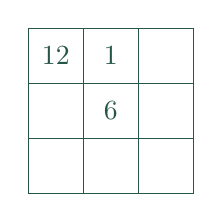
\begin{tikzpicture}[color=thachthuctoanhoc, scale=0.7]
			\draw (0,0) grid (3,3);
			\draw (0.5,2.5) node {$12$};
			\draw (1.5,2.5) node {$1$};
			\draw (1.5,1.5) node {$6$};
		\end{tikzpicture}
		\vspace*{-10pt}
	\end{figure}
	\textbf{\color{thachthuctoanhoc}Lời giải} (\textit{dựa theo ý giải của tất cả lời giải Tạp chí đã nhận được từ bạn đọc})\textbf{\color{thachthuctoanhoc}.}
	\vskip 0.05cm
	Ký hiệu $x$, $a$, $b$, $c$, $d$, $e$ là các số dương được điền vào các ô chưa có số của bảng đã cho, như ở hình dưới đây:
	\begin{figure}[H]
		\vspace*{-5pt}
		\centering
		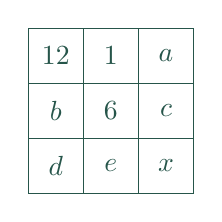
\begin{tikzpicture}[color=thachthuctoanhoc, scale=0.7]
			\draw (0,0) grid (3,3);
			\draw (0.5,2.5) node {$12$};
			\draw (1.5,2.5) node {$1$};
			\draw (1.5,1.5) node {$6$};
			\draw (1.5,0.5) node {$e$};
			\draw (2.5,2.5) node {$a$};
			\draw (2.5,1.5) node {$c$};
			\draw (2.5,0.5) node {$x$};
			\draw (0.5,1.5) node {$b$};
			\draw (0.5,0.5) node {$d$};
		\end{tikzpicture}
		\vspace*{-10pt}
	\end{figure}
	Khi đó, tích các số ở mỗi hàng, mỗi cột, mỗi đường chéo chính của bảng đều bằng \linebreak$12 \cdot 6 \cdot x = 72x$.  Do đó
	\begin{align*}
		a = 72x:\left( {12 \cdot 1} \right) = 6x;
	\end{align*}
	suy ra
	\begin{align*}
		d = 72x:\left( {a \cdot 6} \right) = 72x:\left( {6x \cdot 6} \right) = 2.
	\end{align*}
	Do đó, $e = 72x:\left( {d \cdot x} \right) = 72x:\left( {2 \cdot x} \right) = 36$.
	\vskip 0.05cm
	Vì thế, từ việc xét cột thứ hai của bảng, ta được: tích các số ở mỗi hàng, mỗi cột, mỗi đường chéo chính của bảng đều bằng $1\cdot 6\cdot 36 = 216$. Suy ra
	\begin{align*}
		&x = 216:72 = 3;\,\,\, a = 6x = 6 \cdot 3 = 18;\\
		&c = 216:\left( {a \cdot x} \right) = 216:\left( {18 \cdot 3} \right) = 4;\\
		&b = 216:\left( {12 \cdot d} \right) = 216:\left( {12 \cdot 2} \right) = 9.
	\end{align*}
	Vậy, các số dương được dùng để điền vào bảng, sao cho yêu cầu của đề bài được thỏa mãn, là $18$, $9$, $4$, $2$, $36$, $3$, và chúng được điền như ở bảng ở cột bên:
	\begin{figure}[H]
%		\vspace*{-5pt}
		\centering
		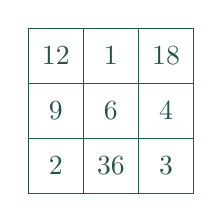
\begin{tikzpicture}[color=thachthuctoanhoc, scale=0.7]
			\draw (0,0) grid (3,3);
			\draw (0.5,2.5) node {$12$};
			\draw (1.5,2.5) node {$1$};
			\draw (1.5,1.5) node {$6$};
			\draw (1.5,0.5) node {$36$};
			\draw (2.5,2.5) node {$18$};
			\draw (2.5,1.5) node {$4$};
			\draw (2.5,0.5) node {$3$};
			\draw (0.5,1.5) node {$9$};
			\draw (0.5,0.5) node {$2$};
		\end{tikzpicture}
		\vspace*{-10pt}
	\end{figure}
	\textbf{\color{thachthuctoanhoc}Bình luận và Nhận xét}
	\vskip 0.05cm
	$\pmb{1.}$ Bài đã ra là một bài toán nhẹ nhàng, ở mức bài ``Đố vui" dành cho học sinh khá, giỏi Toán lớp cuối cấp Tiểu học.
	\vskip 0.05cm
	$\pmb{2.}$ Tất cả các lời giải Tạp chí nhận được từ bạn đọc đều là lời giải đúng.
	\vskip 0.05cm
	\hfill	\textbf{\color{thachthuctoanhoc}Lê Huy}
	\vskip 0.05cm
	{\color{thachthuctoanhoc}{\usefont{T5}{qag}{b}{n} P602.}}
	(Mức $B$) Các số tự nhiên từ $1$ đến $2022$ được viết liền nhau tạo thành số $A$ dưới~đây
	\begin{align*}
		A=1234567891011\ldots 20212022.
	\end{align*}
	Nhân chữ số đầu tiên của $A$ với $2$, rồi cộng với chữ số thứ hai; nhân kết quả thu được với $2$, rồi cộng với chữ số thứ ba; tiếp theo, nhân kết quả thu được với $2$, rồi cộng với chữ số thứ tư; $\ldots$; cứ tiếp tục như thế cho đến chữ số cuối cùng của $A$. Với số mới thu được, lại làm như thế; và cứ tiếp tục làm như vậy cho đến khi thu được số có một chữ số. Hỏi, số có một chữ số thu được là số nào?
	\vskip 0.05cm
	\textbf{\color{thachthuctoanhoc}Lời giải} (\textit{dựa theo Đáp án của bài toán do Tạp chí cung cấp})\textbf{\color{thachthuctoanhoc}.}
	\vskip 0.05cm
	Để tiện cho việc diễn đạt, ta gọi toàn bộ quá trình ``nhân chữ số đầu tiên của một số tự nhiên, có ít nhất hai chữ số, với $2$, rồi cộng với chữ số thứ hai; tiếp theo, nhân kết quả thu được với $2$, rồi cộng với chữ số thứ ba; \ldots; cứ tiếp tục như thế cho đến chữ số cuối cùng của số ấy" là \textit{phép nhân -- cộng}.
	\vskip 0.05cm
	Ta có Nhận xét sau:
	\vskip 0.01cm
	\textbf{\color{thachthuctoanhoc}Nhận xét.} Sau khi thực hiện phép nhân -- cộng đối với số $N \!=\! \overline {{a_n}{a_{n - 1}} \ldots {a_1}{a_0}} $ ($n \!\in\! \mathbb{N^*}$, $n \ge 2, a_n \ne 0$) tùy ý, ta sẽ thu được số
	\begin{align*}
		N' \!=\! {a_n} \!\cdot\! {2^n} \!+\! {a_{n \!-\! 1}} \!\cdot\! {2^{n \!-\! 1}} \!+\!  \!\cdots\!  +\! {a_1} \!\cdot\! {2^1} \!+\! {a_0} \!\cdot\! {2^0}.
	\end{align*}
	Có thể dễ dàng chứng minh Nhận xét trên, bằng phương pháp quy nạp theo $n \ge 2$ (chứng minh cụ thể xin dành cho bạn đọc).
	\vskip 0.01cm
	Do
	\begin{align*}
		&{a_n} \!\cdot\! {2^n} \!+\! {a_{n - 1}} \!\cdot\! {2^{n \!-\! 1}} \!+\!  \cdots  \!+\! {a_1} \!\cdot\! {2^1} \!+\! {a_0} \!\cdot\! {2^0} \\[-0.4ex]
		< \,\,&{a_n} \cdot {10^n} + {a_{n - 1}} \cdot {10^{n - 1}} +  \cdots  \\[-0.4ex]
		&+ {a_1} \cdot {10^1} + {a_0} \cdot {10^0},
	\end{align*}
	nên từ Nhận xét suy ra, nếu $N'$  là số nguyên dương, nhận được từ số nguyên dương N nhờ phép nhân -- cộng, thì
	\begin{align*}
		N > N' > 0.
	\end{align*}
	Vì thế, trong quá trình thực hiện liên tiếp phép nhân -- cộng đối với số $A$, ta sẽ lần lượt nhận được các số nguyên dương   $A_1, A_2, \ldots$, thỏa mãn:
	\begin{align*}
		A > {A_1} > {A_2} >  \cdots  > 0.
	\end{align*}
	Từ đây, do chỉ có hữu hạn số nguyên dương thuộc nửa khoảng $(0; A]$, suy ra, quá trình thực hiện liên tiếp phép nhân -- cộng đối với số $A$ chỉ có thể gồm hữu hạn lần thực hiện phép đó. Nói một cách khác, tồn tại số nguyên dương $k$, sao cho sau $k$ lần thực hiện liên tiếp phép nhân -- cộng đối với số $A$, sẽ thu được một số tự nhiên, mà đối với nó, không thể thực hiện phép nhân -- cộng; ký hiệu số này là $A_k$.
	\vskip 0.01cm
	Từ định nghĩa phép nhân -- cộng, hiển nhiên thấy, ta không thể thực hiện phép đó đối với một số tự nhiên khi và chỉ khi số tự nhiên ấy là số có một chữ số. Do đó, $A_k$  là số có một chữ số.
	\vskip 0.01cm
	Như vậy, bằng cách thực hiện liên tiếp phép nhân -- cộng đối với số $A$, ta chắc chắn thu được một số tự nhiên có một chữ số.
	\vskip 0.01cm
	Tiếp theo, do
	\begin{align*}
			&\left({a_n} \cdot {{10}^n} + {a_{n - 1}} \cdot {{10}^{n - 1}} +  \cdots  + {a_1} \cdot {{10}^1}\right. \\[-0.4ex]
			&\left.+ {a_0} \cdot {{10}^0} \right) - \left( {a_n} \cdot {2^n} + {a_{n - 1}} \cdot {2^{n - 1}} +  \cdots\right. \\[-0.4ex]
			&\left.+ {a_1} \cdot {2^1} + {a_0} \cdot {2^0} \right)\\[-0.4ex]
			=\, &{a_n} \cdot \left( {{{10}^n} - {2^n}} \right) + {a_{n - 1}} \cdot \left( {{{10}^{n - 1}} - {2^{n - 1}}} \right) \\[-0.4ex]
			&+  \cdots + {a_1} \cdot \left( {{{10}^1} - {2^1}} \right) \equiv 0\left( {\bmod 8} \right),
	\end{align*}
	nên từ Nhận xét suy ra, nếu  $N'$ là số nguyên dương, nhận được từ số nguyên dương $N$ nhờ phép nhân -- cộng, thì
	\begin{align*}
		N \equiv N'\left( {\bmod 8} \right).
	\end{align*}
	Vì thế, ta có
	\begin{align*}
		A \equiv {A_1} \equiv {A_2} \equiv  \cdots  \equiv {A_k}\left( {\bmod 8} \right).
	\end{align*}
	Từ đó, vì
	\begin{align*}
		A &= 1234567891011 \ldots 20212 \cdot {10^3} + 22 \\[-0.4ex]
		&\equiv 22 \equiv 6\left( {\bmod 8} \right),
	\end{align*}
	nên ${A_k} \equiv 6\left( {\bmod 8} \right)$.  Mà  $A_k$ là số có một chữ số, nên $A_k = 6$.
	\vskip 0.05cm 
	Vậy, bằng cách thực hiện liên tiếp phép nhân -- cộng đối với số $A$, ta sẽ thu được một số tự nhiên có một chữ số; và số đó là $6$.
	\vskip 0.05cm
	\textbf{\color{thachthuctoanhoc}Bình luận và Nhận xét}
	\vskip 0.05cm
	$\pmb{1.}$ Trong đề bài, câu ``\textit{cứ tiếp tục làm như vậy cho đến khi thu được số có một chữ số}" chỉ thể hiện trạng thái, mà nếu gặp nó, ta sẽ kết thúc quá trình thực hiện liên tiếp phép nhân -- cộng, chứ không thể hiện trạng thái, mà ta chắc chắn sẽ thu được, sau một số hữu hạn lần thực hiện liên tiếp phép đó đối với số $A$. Hơn nữa, việc sẽ thu được hay không thể thu được một trạng thái như thế không là điều hiển nhiên, hoặc dễ thấy. Vì thế, trong lời giải của bài toán, bắt buộc phải trình bày các lập luận, khẳng định thu được hay không thể thu được số có một chữ số, nhờ việc thực hiện liên tiếp phép nhân -- cộng đối với số $A$.
	\vskip 0.05cm
	$\pmb{2.}$ Tạp chí đã nhận được $05$ (năm) lời giải, từ bạn đọc; ở tất cả các lời giải này, đều thiếu phần lập luận vừa nêu trên.
	\vskip 0.05cm
	\hfill	\textbf{\color{thachthuctoanhoc}Nguyễn Khắc Minh}
	\vskip 0.1cm
	{\color{thachthuctoanhoc}{\usefont{T5}{qag}{b}{n} P603.}}
	(Mức $B$) Lấy $n$ điểm tuỳ ý ($n\in\mathbb N^*$, $n\ge2$) nằm bên trong một hình chữ nhật kích thước  $3 \times 6$. 
	\vskip 0.05cm
	$a)$ Với $n=5$, chứng minh rằng trong các điểm đã lấy, tồn tại hai điểm mà khoảng cách giữa chúng không lớn hơn $\sqrt{10}$. 
	\vskip 0.05cm
	$b)$ Khẳng định ở câu $a)$ còn đúng không, nếu  $n=4$?
	\vskip 0.05cm
	\textbf{\color{thachthuctoanhoc}Lời giải} (\textit{của người chấm bài})\textbf{\color{thachthuctoanhoc}.}
	\vskip 0.05cm
	$a)$ Trước hết, ta nhắc lại kết quả cơ bản, quen thuộc sau:
	\vskip 0.05cm
	\textbf{\color{thachthuctoanhoc}Bổ đề.} Khoảng cách giữa hai điểm tùy ý, thuộc cùng một hình chữ nhật, không vượt quá độ dài đường chéo của hình chữ nhật ấy.
	\vskip 0.05cm
	\textit{Trở lại bài toán.}
	\vskip 0.05cm
	Chia hình chữ nhật đã cho thành hai hình vuông kích thước $3\times 3$, hình vuông màu xanh và hình vuông màu trắng, như ở Hình~$1$. Khi đó, theo nguyên lý Dirichlet, trong $5$ điểm đã lấy, tồn tại $3$ điểm cùng thuộc một hình vuông. Không mất tổng quát, giả sử $3$ điểm đó cùng thuộc hình vuông màu trắng. Chia hình vuông này thành các hình vuông đơn vị (xem Hình $2$). Khi đó, ta sẽ có một bảng ô vuông kích thước $3\times 3$ (bảng có $3$ hàng và $3$ cột).	
	\begin{figure}[H]
		\centering
		\vspace*{-10pt}
		\captionsetup{labelformat= empty, justification=centering}
		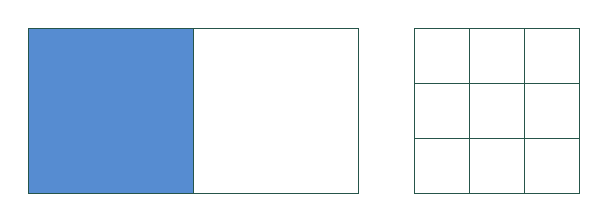
\begin{tikzpicture}[scale=0.7,color=thachthuctoanhoc]
			\filldraw [cackithi] (0,0) rectangle (3,3);
			\draw (0,0) rectangle (6,3);
			\draw (3,0) rectangle (3,3);
			\draw (7,0) grid (10,3);
		\end{tikzpicture}
		\caption{\small\textit{\color{thachthuctoanhoc}\hspace*{35pt} Hình $1$ \hspace*{70pt} Hình $2$}}
		\vspace*{-15pt}
	\end{figure}
	Xảy ra một trong hai trường hợp sau:
	\vskip 0.05cm
	$\bullet$ \textit{Trường hợp $1$: Trong ba điểm, tồn tại hai điểm thuộc cùng một hàng, hoặc cùng một cột.} Khi đó, hai điểm này sẽ thuộc một hình chữ nhật kích thước $1\times 3$, hoặc $3\times 1$. Do đó, theo Bổ đề, khoảng cách giữa chúng không vượt quá $\sqrt{3^2 + 1^2} = \sqrt{10}$.
	\vskip 0.05cm
	$\bullet$ \textit{Trường hợp $2$: Trong ba điểm, không có hai điểm nào thuộc cùng một hàng, hoặc cùng một cột.} Khi đó, ở mỗi hàng, cũng như ở mỗi cột, đều có đúng một điểm.
	\vskip 0.05cm
	Xét điểm thuộc cột $1$ và điểm thuộc cột $2$ (thứ tự của các cột được tính từ trái qua phải).
	\vskip 0.05cm
	-- \textit{Nếu hai điểm này thuộc hai hàng kề nhau} thì chúng sẽ cùng thuộc hoặc hình vuông $2\times 2$ màu hồng ở Hình $3$, hoặc hình vuông $2\times 2$ màu hồng ở Hình $4$. Bất luận thuộc hình vuông nào, khoảng cách giữa chúng, theo Bổ đề, không vượt quá
	\begin{align*}
		\sqrt {{2^2} + {2^2}}  = \sqrt 8  < \sqrt {10} .
	\end{align*}
	\begin{figure}[H]
		\centering
%		\vspace*{5pt}
		\captionsetup{labelformat= empty, justification=centering}
		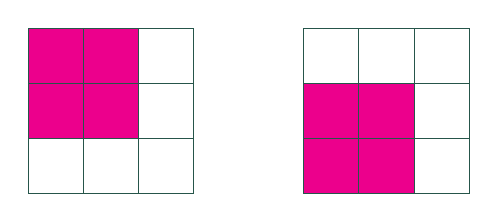
\begin{tikzpicture}[scale=0.7,color=thachthuctoanhoc]
			\filldraw [toancuabi] (0,1) rectangle (2,3);
			\filldraw [toancuabi] (5,0) rectangle (7,2);
			\draw (0,0) grid (3,3);
			\draw (5,0) grid (8,3);
		\end{tikzpicture}
		\caption{\small\textit{\color{thachthuctoanhoc}Hình $3$ \hspace*{60pt} Hình $4$}}
		\vspace*{-10pt}
	\end{figure}
	-- \textit{Nếu điểm thuộc cột $1$ và điểm thuộc cột $2$ thuộc hai hàng không kề nhau} thì một điểm sẽ thuộc hàng $1$ và một điểm thuộc hàng $3$ (thứ tự của các hàng được tính từ trên xuống dưới). Do đó, điểm còn lại, trong ba điểm, sẽ thuộc ô vuông con nằm ở giao của hàng $2$ và cột $3$. Vì thế, điểm này và điểm thuộc cột $2$ cùng thuộc hoặc hoặc hình vuông $2\times 2$ màu hồng ở Hình $5$, hoặc hình vuông $2\times 2$ màu hồng ở Hình $6$. Bất luận thuộc hình vuông nào, khoảng cách giữa chúng, theo Bổ đề, không vượt quá
	\begin{align*}
		\sqrt {{2^2} + {2^2}}  = \sqrt 8  < \sqrt {10}.
	\end{align*}
	\begin{figure}[H]
		\centering
		\vspace*{-10pt}
		\captionsetup{labelformat= empty, justification=centering}
		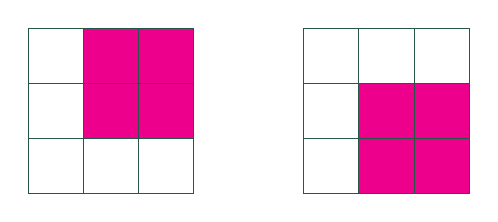
\begin{tikzpicture}[scale=0.7,color=thachthuctoanhoc]
			\filldraw [toancuabi] (1,1) rectangle (3,3);
			\filldraw [toancuabi] (6,0) rectangle (8,2);
			\draw (0,0) grid (3,3);
			\draw (5,0) grid (8,3);
		\end{tikzpicture}
		\caption{\small\textit{\color{thachthuctoanhoc}Hình $5$ \hspace*{60pt} Hình $6.$}}
		\vspace*{-10pt}
	\end{figure}
	Kết quả xét hai trường hợp nêu trên cho thấy, trong ba điểm thuộc hình vuông $3\times 3$ màu trắng, tồn tại hai điểm có khoảng cách không vượt quá  $\sqrt{10}$. Vì thế, ta có điều phải chứng minh theo yêu cầu đề bài.
	\vskip 0.05cm
	$b)$ Xét hình chữ nhật kích thước $2,97\times 5,94$ nằm trong hình chữ nhật đã cho. Chia hình chữ nhật đó thành các hình vuông kích thước $0,99\times 0,99$, và lấy bốn điểm $A$, $B$, $C$, $D$, như ở Hình $7$. Bốn điểm này, hiển nhiên, nằm bên trong hình chữ nhật đã cho.
	\begin{figure}[H]
		\centering
		\vspace*{-10pt}
		\captionsetup{labelformat= empty, justification=centering}
		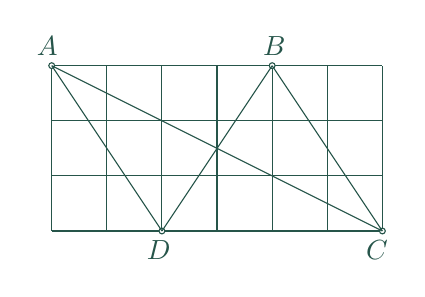
\begin{tikzpicture}[scale=0.7,color=thachthuctoanhoc]
			\draw (0,0) grid (6,3);
			\draw [fill=white] (6.,0.) circle (1.5pt);
			\draw (5.9,-0.35) node {$C$};
			\draw [fill=white] (0.,3.) circle (1.5pt);
			\draw (-0.08,3.35) node {$A$};
			\draw [fill=white] (2.,0.) circle (1.5pt);
			\draw (1.94,-0.35) node {$D$};
			\draw [fill=white] (4.,3.) circle (1.5pt);
			\draw (4.04,3.35) node {$B$};
			\draw (0,3)--(2,0) (0,3) -- (6,0) (2,0) -- (4,3) (4,3) -- (6,0);
		\end{tikzpicture}
		\caption{\small\textit{\color{thachthuctoanhoc}Hình $7$}}
		\vspace*{-5pt}
	\end{figure}
	Ta có:
	\begin{align*}
		AB &= CD = 0,99 \cdot 4 = 3,96 > \sqrt {10} .\\
		AD &= DB = BC = \sqrt {\!{{\left( {0,99 \!\cdot\! 2} \right)}^2} \!+\! {{\left( {0,99 \!\cdot\! 3} \right)}^2}}  \\
		&= 0,99 \cdot \sqrt {13}  > \sqrt {10} .\\
		AC &= \sqrt {2,{{97}^2} \!+\! 5,{{94}^2}}  = 2,97 \!\cdot\! \sqrt 5  >\! \sqrt {10}.
	\end{align*}
	Như vậy, khoảng cách giữa hai điểm bất kỳ, trong bốn điểm $A$, $B$, $C$, $D$, đều lớn hơn  $\sqrt{10}$. Vì thế, khẳng định ở câu $a)$ \textit{không} còn đúng, nếu $n = 4$.
	\vskip 0.05cm
	\textbf{\color{thachthuctoanhoc}Bình luận và Nhận xét}
	\vskip 0.05cm
	$\pmb{1.}$ Từ lời giải trên, dễ thấy, ở câu $a)$, với giả thiết ``năm điểm được lấy nằm \textit{bên trong} hình chữ nhật $3\times 6$", ta có thể chứng minh được khẳng định mạnh hơn khẳng định của đề bài. Đó là, trong năm điểm ấy, tồn tại hai điểm có khoảng cách \textit{nhỏ hơn} $\sqrt{10}$.
	\vskip 0.05cm 
	$\pmb{2.}$ Rất tiếc, tất cả các lời giải Tạp chí đã nhận được từ bạn đọc đều có lời giải câu $b)$ hoặc sai (do bốn điểm được lấy nằm trên biên của hình chữ nhật $3\times 6$, trong khi đề bài yêu cầu các điểm được lấy phải nằm bên trong hình chữ nhật đó), hoặc ``lơ mơ" (do người giải bài chỉ mô tả các điểm được lấy, mà không có bất cứ chứng cứ nào cho thấy, khoảng cách giữa hai điểm tùy ý trong các điểm ấy lớn hơn  $\sqrt{10}$).
	\vskip 0.05cm
	\hfill	\textbf{\color{thachthuctoanhoc}Hà Thanh}
	\vskip 0.05cm
	{\color{thachthuctoanhoc}{\usefont{T5}{qag}{b}{n} P604.}}
	(Mức $B$) Cho $a, b, c$ là các số thực không âm thỏa mãn $a b+b c+c a=1$. Chứng minh rằng
	\begin{align*}
		&a \sqrt{b^{2}+b c+c^{2}}+b \sqrt{c^{2}+c a+a^{2}}\\
		&+c \sqrt{a^{2}+a b+b^{2}} \le a+b+c .
	\end{align*}
	Dấu ``$=$" xảy ra khi nào?
	\vskip 0.05cm
	\textbf{\color{thachthuctoanhoc}Lời giải} (\textit{phỏng theo lời giải của các bạn Trần Đình Nam, lớp $10$T$2$, trường THPT chuyên Lê Hồng Phong, tỉnh Nam Định, và Nguyễn Chí Việt Khang, lớp $11$T$1$, trường THPT chuyên Nguyễn Quang Diêu, tỉnh Đồng Tháp})\textbf{\color{thachthuctoanhoc}.}
	\vskip 0.05cm
	Áp dụng bất đẳng thức trung bình cộng -- trung bình nhân cho hai số thực không âm  $\sqrt {{b^2} + bc + {c^2}} $ và $1$, với lưu ý tới giả thiết của đề bài, ta được:
	\begin{align*}
		&\sqrt {{b^2} + bc + {c^2}}  \le \frac{{\left( {{b^2} + bc + {c^2}} \right) + 1}}{2} \\
		= &\frac{{\left( {{b^2} + bc + {c^2}} \right) + \left( {ab + bc + ca} \right)}}{2} \\
		= &\frac{{\left( {b + c} \right)\left( {a + b + c} \right)}}{2}.
	\end{align*}
	Suy ra 
	\begin{align*}
		&a\sqrt {{b^2} + bc + {c^2}}  \\
		\le\, &\frac{{a\left( {b + c} \right)\left( {a + b + c} \right)}}{2} \quad(\text{\color{black}do } a \ge 0). \tag{$1$}
	\end{align*}
	Bằng cách hoàn toàn tương tự, ta cũng chứng minh được:
	\begin{align*}
		&b\sqrt {\!{c^2} \!+\! ca \!+\! {a^2}} \le\! \frac{{b\left( {c \!+\! a} \right)\left( {a \!+\! b \!+\! c} \right)}}{2}.\tag{$2$}\\
		&c\sqrt {\!{a^2} \!+\! ab \!+\! {b^2}} \le\! \frac{{c\left( {a \!+\! b} \right)\left(\!{a \!+\! b \!+\! c} \right)}}{2}.\tag{$3$}
	\end{align*}
	Cộng các bất đẳng thức ($1$), ($2$), ($3$), vế theo vế, ta được:
	\begin{align*}
		&a\sqrt {{b^2} + bc + {c^2}}  + b\sqrt {{c^2} + ca + {a^2}}  \\
		&+ c\sqrt {{a^2} + ab + {b^2}}  \\
		\le &\left( {ab \!+\! bc \!+\! ca} \right)\!\left( {a \!+\! b \!+\! c} \right) \!=\! a \!+\! b \!+\! c \tag{$4$}
	\end{align*}
	(do $ab + bc + ca = 1$).
	\vskip 0.05cm
	Ta có điều phải chứng minh theo yêu cầu đề bài.
	\vskip 0.05cm
	Đẳng thức ở ($4$) xảy ra khi và chỉ khi đẳng thức xảy ra đồng thời ở ($1$), ($2$) và ($3$).                    \hfill ($5$)
	\vskip 0.05cm
	Với $ab + bc + ca = 1$, ta có:
	\vskip 0.05cm
	-- Đẳng thức ở ($1$) xảy ra khi và chi khi $a = 0$, hoặc $b^2 + bc + c^2 = 1$. 
	\vskip 0.05cm 
	-- Đẳng thức ở ($2$) xảy ra khi và chi khi $b = 0$, hoặc  $c^2 + ca + a^2 = 1$.
	\vskip 0.05cm
	-- Đẳng thức ở ($3$) xảy ra khi và chi khi $c = 0$, hoặc  $a^2 + ab + b^2 = 1$.
	\vskip 0.05cm
	Vì $ab + bc + ca = 1$ nên trong ba số $a$, $b$, $c$ chỉ có thể có tối đa một số bằng $0$. Do đó, từ ($5$) và các điều kiện xảy ra đẳng thức ở ($1$), ($2$), ($3$), ta được: đẳng thức ở ($4$) xảy ra khi và chỉ khi ta có một trong các điều ($I$), ($II$), ($III$), ($IV$) sau:
	\begin{align*}
		(I)\begin{cases}
			a,b,c \ge 0\\[-0.5ex]
			ab + bc + ca = 1\\[-0.5ex] 
			a = 0\\[-0.5ex]
			{c^2} + ca + {a^2} = {a^2} + ab + {b^2} = 1.
		\end{cases}
	\end{align*}
	\begin{align*}
		(II)\begin{cases}
			a,b,c \ge 0\\[-0.5ex]
			ab + bc + ca = 1\\[-0.5ex]
			b = 0\\[-0.5ex]
			{b^2} + bc + {c^2} = {a^2} + ab + {b^2} = 1.
		\end{cases}
	\end{align*}
	\begin{align*}
		(III)\begin{cases}
			a,b,c \ge 0\\[-0.5ex]
			ab + bc + ca = 1\\[-0.5ex]
			c = 0\\[-0.5ex]
			{b^2} + bc + {c^2} = {c^2} + ca + {a^2} = 1.
		\end{cases}
	\end{align*}
	\begin{align*}
		(IV)\begin{cases}
				a,b,c \ge 0\\[-0.5ex]
				ab + bc + ca = 1\\[-0.5ex]
				abc \ne 0\\[-0.5ex]
				{b^2} + bc + {c^2} = {c^2} + ca + {a^2} \\[-0.5ex]
				\quad\quad\quad\quad\quad= {a^2} + ab + {b^2} = 1.
		\end{cases}
	\end{align*}
	Dễ thấy:
	\begin{align*}
		&(I) \Leftrightarrow a = 0 \text{ và } b = c = 1;\\[-0.5ex]
		&(II) \Leftrightarrow b = 0 \text{ và } c = a = 1;\\[-0.5ex]
		&(III) \Leftrightarrow c = 0 \text{ và } a = b = 1;\\[-0.5ex]
		&(IV) \Leftrightarrow a=b=c= \frac{1}{\sqrt{3}}.
	\end{align*}
	Vậy, dấu ``$=$" ở bất đẳng thức của đề bài xảy ra khi và chỉ khi một trong ba số $a$, $b$, $c$ bằng $0$ và hai số còn lại bằng $1$, hoặc cả ba số đó cùng bằng  $\frac{1}{\sqrt{3}}$.
	\vskip 0.05cm
	\textbf{\color{thachthuctoanhoc}Bình luận và Nhận xét}
	\vskip 0.05cm
	Tạp chí đã nhận được $10$ lời giải, từ bạn đọc. Rất tiếc, trong số này, có một lời giải sai, do người giải bài đã biến đổi sai một số biểu thức; đa phần các lời giải còn lại đều sai phần xét khả năng xảy ra dấu đẳng thức ở bất đẳng thức của đề bài, do người giải bài xử lý không đúng điều kiện xảy ra dấu đẳng thức ở bất đẳng thức Cauchy -- Bunyakovsky -- Schwarz.
	\vskip 0.05cm
	\hfill	\textbf{\color{thachthuctoanhoc}Lưu Thị Thanh Hà}
	\vskip 0.01cm
	{\color{thachthuctoanhoc}{\usefont{T5}{qag}{b}{n} P605.}}
	(Mức $B$) Cho tam giác $ABC$ cân tại $A$, có đường cao $AD$. Gọi $E$ là trung điểm $AD$; $F,G$ là hình chiếu vuông góc của $D$ trên $AC,BE$. Đường thẳng $GC$ cắt các đường thẳng $DF$ và $BF$ tương ứng tại $H$ và $I$. Chứng minh rằng $\angle{GAH}+\angle{GIF}=180^\circ$.  
	\vskip 0.05cm
	\textbf{\color{thachthuctoanhoc}Lời giải} (\textit{của người chấm bài})\textbf{\color{thachthuctoanhoc}.}
	\begin{figure}[H]
		\vspace*{-10pt}
		\centering
		\captionsetup{labelformat= empty, justification=centering}
		\includegraphics[width= 0.85\linewidth]{P605}
		\vspace*{-10pt}
	\end{figure}
	Gọi $K$ là giao điểm của $AH$ và $BF$. Ta sẽ chứng minh $AGIK$ là tứ giác nội tiếp.
	\vskip 0.05cm
	Do $DG \bot BE$ và $AD \bot BC$ (giả thiết), nên
	\begin{align*}
		\angle DBG = \angle EDG\tag{$1$}
	\end{align*}
	(hai góc nhọn có cạnh tương ứng vuông góc).
	\vskip 0.05cm
	Do đó, tam giác vuông $BDG$ đồng dạng với tam giác vuông $DEG$. Từ đây, vì $E$ là trung điểm của $AD$, và $D$ là trung điểm của $BC$ (do tam giác $ABC$ cân tại $A$), suy ra
	\begin{align*}
		\frac{{BC}}{{BG}} = \frac{{2BD}}{{BG}} = \frac{{2DE}}{{DG}} = \frac{{DA}}{{DG}}. \tag{$2$}
	\end{align*}
	Từ ($1$) và ($2$) suy ra,
	\begin{align*}
		\Delta GBC \sim \Delta GDA \,\,\,\text{\color{black}(c.g.c)}. \tag{$3$}
	\end{align*}
	Do đó
	\begin{align*}
		&\angle DGA = \angle BGC, \tag{$4$}\\
		&\angle DCG = \angle BCG = \angle DAG.\tag{$5$}
	\end{align*}
	Từ ($4$) suy ra
	\begin{align*}
		\angle IGA &= \angle CGA = \angle DGA - \angle DGC \\
		&= \angle BGC - \angle DGC \\
		&= \angle BGD = {90^{\circ}}. \tag{$6$}
	\end{align*}
	Từ ($5$), do $A$ và $C$ nằm cùng phía đối với $GD$, suy ra, $AGDC$ là tứ giác nội tiếp. Do đó, với lưu ý tới ($4$), ta có:
	\begin{align*}
		\angle EGH &= {180^{\circ}} - \angle BGC \\
		&= {180^{\circ}} - \angle DGA = \angle DCA. \tag{$7$}
	\end{align*}
	Do $ED \bot DC$ và $DH \bot CA$ (giả thiết), nên
	\begin{align*}
		\angle EDH = \angle DCA  \tag{$8$}
	\end{align*}
	(hai góc nhọn có cạnh tương ứng vuông góc).
	\vskip 0.05cm
	Từ ($7$) và ($8$) suy ra, $\angle EGH = \angle EDH$; do đó, $EGDH$ là tứ giác nội tiếp. Suy ra
	\begin{align*}
		\angle DHE \!=\!\! {180^{\circ}} \!-\! \angle EGD \!=\! {180^{\circ}} \!\!-\! {90^{\circ}} \!=\! {90^{\circ}}.
	\end{align*}
	Vì thế, $EH \bot DF$; suy ra, $EH \parallel AF$. Mà $E$ là trung điểm của $AD$, nên $H$ là trung điểm của $DF$. Suy ra
	\begin{align*}
		DF = 2DH.                     \tag{$9$}
	\end{align*}
	Từ ($7$) suy ra, tam giác vuông $DFA$ đồng dạng với tam giác vuông $CFD$. Do đó, với lưu ý tới ($9$), ta có:
	\begin{align*}
		\frac{{DA}}{{DH}} = \frac{{2DA}}{{DF}} = \frac{{2CD}}{{CF}} = \frac{{CB}}{{CF}}.
	\end{align*}
	Từ đây và ($8$) suy ra, $\Delta BCF \sim \Delta ADH$. Do đó
	\begin{align*}
		\angle DBK = \angle CBF = \angle DAH = \angle DAK.
	\end{align*}
	Mà $A$, $B$ nằm cùng phía đối với $DK$, nên $ABDK$ là tứ giác nội tiếp. Vì thế
	\begin{align*}
		\angle AKI = \angle AKB = \angle ADB = 90^{\circ}. \tag{$10$}
	\end{align*}
	Từ ($6$) và ($10$) suy ra, $AGIK$ là tứ giác nội tiếp. Từ đây, hiển nhiên ta có điều phải chứng minh theo yêu cầu đề bài.
	\vskip 0.05cm
	\textbf{\color{thachthuctoanhoc}Bình luận và Nhận xét}
	\vskip 0.05cm
	$\pmb{1.}$ Bài đã ra là một bài toán thú vị, rất hữu ích cho các bạn học sinh khá, giỏi toán cấp THCS, cũng như cấp THPT, trong việc rèn luyện tư duy hình học và kỹ năng giải toán hình học.
	\vskip 0.05cm
	$\pmb{2.}$ Tất cả các lời giải Tạp chí nhận được từ bạn đọc đều là lời giải đúng và hoàn chỉnh.
	\begin{flushright}
		\textbf{\color{thachthuctoanhoc}Hạ Vũ Anh}
	\end{flushright}
	{\color{thachthuctoanhoc}{\usefont{T5}{qag}{b}{n} P606.}}
	(Mức $B$) Giải hệ phương trình 
	\begin{align*}
		\begin{cases}
			\dfrac{x}{y}+\sqrt{x}&=y+\sqrt{\dfrac{y}{x}},
			\\x y+x+y&=3.
		\end{cases}
	\end{align*}
	\textbf{\color{thachthuctoanhoc}Lời giải} $\pmb{1}$ (\textit{phỏng theo ý giải của một bạn học sinh cấp THCS})\textbf{\color{thachthuctoanhoc}.}
	\vskip 0.05cm
	Điều kiện xác định của hệ phương trình: $x, y > 0$.
	\vskip 0.05cm
	$\bullet$ Dễ thấy, nếu $(x; y)$ là cặp số thực dương, mà $x \ge 3$, hoặc $y \ge 3$, thì $xy + x + y > 3$. Vì thế, trong các cặp số thực dương như vậy, không có cặp số nào là nghiệm của hệ phương trình đã cho.
	\vskip 0.05cm
	$\bullet$ Xét các cặp số thực dương $(x; y)$, mà \linebreak$0 < x, y < 3$.
	\vskip 0.05cm
	Từ phương trình thứ hai của hệ đã cho, suy ra
	\begin{align*}
		x = \frac{{3 - y}}{{y + 1}} > 0  \quad(\text{\color{black}do } 0 < y < 3).      \tag{$1.1$}
	\end{align*}
	Thế ($1.1$) vào phương trình thứ nhất của hệ đã cho, ta được:
	\begin{align*}
		\frac{{3 \!-\! y}}{{y\left( {y \!+\! 1} \right)}} \!+\! \sqrt {\frac{{3 \!-\! y}}{{y \!+\! 1}}}  \!=\! y \!+\! \sqrt {\frac{{y\left( {y \!+\! 1} \right)}}{{3 \!-\! y}}}. \tag{$1.2$}
	\end{align*}
	Vì $y \in (0; 3)$ nên
	\begin{align*}
		&\,(1.2) \\
		\Leftrightarrow &\left(\!{\frac{{3 \!-\! y}}{{{y^2} \!+\! y}} \!-\! y}\! \right) \!+\!\! \left(\!\!\!\! {\sqrt {\frac{{\left( {3 \!-\! y} \right)y}}{{{y^2} \!+\! y}}}  \!-\! \sqrt {\frac{{{y^2} \!+\! y}}{{3 \!-\! y}}} } \right) \!\!=\! 0\\
		\Leftrightarrow &\frac{{3 \!-\! y \!-\! {y^2} \!-\! {y^3}}}{{{y^2} \!+\! y}} \!+\! \frac{{\sqrt y \left( {3 \!-\! \sqrt y  \!-\! y \!-\! y\sqrt y } \right)}}{{\sqrt {{y^2} \!+\! y}  \!\cdot\! \sqrt {3 \!-\! y} }} \!=\! 0\\
		\Leftrightarrow&\frac{{\left( {1 - y} \right)\left( {3 + 2y + {y^2}} \right)}}{{{y^2} + y}} \\
		&+ \frac{{\sqrt y \left( {1 - \sqrt y } \right)\left( {3 + 2\sqrt y  + y} \right)}}{{\sqrt {{y^2} + y}  \cdot \sqrt {3 - y} }} = 0\\
		\Leftrightarrow&\left( {1 - \sqrt y } \right)\left( \frac{{\left( {1 + \sqrt y } \right)\left( {3 + 2y + {y^2}} \right)}}{{{y^2} + y}}\right. \\
		&\left.+ \frac{{\sqrt y \left( {3 + 2\sqrt y  + y} \right)}}{{\sqrt {{y^2} + y}  \cdot \sqrt {3 - y} }} \right) = 0. \tag{$1.3$}
	\end{align*}
	Do
	\begin{align*}
		&\frac{{\left( {1 + \sqrt y } \right)\left( {3 + 2y + {y^2}} \right)}}{{{y^2} + y}} \\
		&+ \frac{{\sqrt y \left( {3 + 2\sqrt y  + y} \right)}}{{\sqrt {{y^2} + y}  \cdot \sqrt {3 - y} }} > 0 \quad\forall y \in \left( {0;3} \right),
	\end{align*}
	nên: ($1.3$) $\Leftrightarrow$ $1- \sqrt{y} = 0 \Leftrightarrow y =1$. \hfill ($1.4$)   
	\vskip 0.05cm
	Thế ($1.4$) vào ($1.1$), ta được $x = 1$.
	\vskip 0.05cm
	Vì cặp số $(x; y) = (1; 1)$ nằm trong số các cặp số đang xét, và thỏa mãn điều kiện xác định, nên nó là nghiệm của hệ phương trình đã cho.
	\vskip 0.05cm
	$\bullet$ Vậy, hệ đã cho có duy nhất nghiệm $(x; y) = (1; 1)$.
	\vskip 0.05cm
	\textbf{\color{thachthuctoanhoc}Lời giải} $\pmb{2}$ (\textit{của người chấm bài})\textbf{\color{thachthuctoanhoc}.}
	\vskip 0.05cm
	Điều kiện xác định của hệ phương trình: $x, y > 0$.
	\vskip 0.05cm
	$\bullet$ Giả sử $\left( {{x_0};{y_0}} \right)$ là một nghiệm của hệ đã cho. Khi đó, ta có $x_0, y_0 > 0$  và
	\begin{align*}
		\quad\,\,\begin{cases}
			\frac{{{x_0}}}{{{y_0}}} + \sqrt {{x_0}}  = {y_0} + \sqrt {\frac{{{y_0}}}{{{x_0}}}} \quad\quad\quad\,\, &\text{\color{black}(}2.1\text{\color{black})}\\
			{x_0}{y_0} + {x_0} + {y_0} = 3.\quad\quad\quad\quad\,\, &\text{\color{black}(}2.2\text{\color{black})}
		\end{cases}
	\end{align*}
	Nhận thấy, với mọi $x, y \!\!>\!\! 0$, nếu $0 \!<\! x, y \!\!<\!\!1$\linebreak thì $xy + x + y < 3$, còn nếu $x, y > 1$ thì $xy + x + y > 3$. Vì thế, từ ($2.2$) suy ra
	\begin{align*}
		 0 < {x_0} < 1 \le {y_0}, \,\text{\color{black} hoặc }  {x_0} \ge 1 \ge {y_0} > 0.
	\end{align*}
	Tiếp theo, dễ thấy, nếu $0 < {x_0} < 1 \le {y_0}$  thì
	\begin{align*}
		\frac{{{x_0}}}{{{y_0}}} + \sqrt {{x_0}}  < 1 + 1 = 2 < {y_0} + \sqrt {\frac{{{y_0}}}{{{x_0}}}},
	\end{align*}
	mâu thuẫn với ($2.1$). Vì vậy, phải có 
	\begin{align*}
		{x_0} \ge 1 \ge {y_0} > 0. \tag{$2.3$}
	\end{align*}
	Do với mọi $x, y$ mà  $x \ge 1 \ge y > 0$, ta có
	\begin{align*}
		\frac{x}{y} + \sqrt x  \ge 1 + 1 = 2 \ge y + \sqrt {\frac{y}{x}},
	\end{align*}
	nên từ ($2.3$) suy ra
	\begin{align*}
		(2.1) &\Leftrightarrow \frac{{{x_0}}}{{{y_0}}} = \sqrt {{x_0}}  = 1 = {y_0} = \sqrt {\frac{{{y_0}}}{{{x_0}}}} \\
		&\Leftrightarrow {x_0} = {y_0} = 1.
	\end{align*}
	Như vậy, nếu $\left( {{x_0};{y_0}} \right)$ là nghiệm của hệ đã cho thì $x_0 = y_0 =1$.
	\vskip 0.05cm  
	$\bullet$ Ngược lại, bằng cách thử trực tiếp, dễ thấy cặp số $(x; y) = (1; 1)$ nghiệm đúng hệ đã cho.
	\vskip 0.05cm
	$\bullet$ Vì vậy, hệ đã cho có duy nhất nghiệm $(x; y) = (1; 1)$.
	\vskip 0.05cm
	\textbf{\color{thachthuctoanhoc}Bình luận và Nhận xét}
	\vskip 0.05cm
	Trong số các lời giải Tạp chí đã nhận được từ bạn đọc:
	\vskip 0.05cm
	-- Rất tiếc, có hai lời giải sai, gồm một lời giải sai do người giải bài đã biến đổi sai phương trình ($1.2$) trong Lời giải $1$ trên đây, và một lời giải sai do người giải bài ngộ nhận rằng, trường hợp $y \ge 1$ được xét tương tự như trường hợp $x \ge 1$. (\textit{Lưu ý các bạn, vai trò của $x$ và $y$ không như nhau trong hệ phương trình đã cho.}).
	\vskip 0.05cm
	-- Có những lời giải cho thấy, người giải bài chưa hiểu đúng về điều kiện xác định của hệ phương trình. Cụ thể, có bạn đã tìm sai điều kiện xác định của hệ phương trình, hay có bạn, sau khi nêu điều kiện xác định của hệ phương trình là ``$x, y > 0$", để giải hệ đã xét hai trường hợp, gồm trường hợp ``$y=-1$" và trường hợp ``$y \ne -1$"!
	\vskip 0.05cm
	-- Nhiều lời giải mắc lỗi không thử lại nghiệm tìm được.
	\begin{flushright}
		\textbf{\color{thachthuctoanhoc}Lưu Thị Thanh Hà}
	\end{flushright}
	{\color{thachthuctoanhoc}{\usefont{T5}{qag}{b}{n} P607.}}
	(Mức $A$) 
	Cho một nhóm có $7$ người, mà với $6$ người bất kỳ của nhóm, luôn có thể xếp họ ngồi quanh một chiếc bàn tròn, sao cho hai người ngồi cạnh nhau là hai người quen nhau. Chứng minh rằng, có thể xếp tất cả $7$ người của nhóm ngồi quanh một chiếc bàn tròn, sao cho hai người ngồi cạnh nhau là hai người quen nhau.
	\vskip 0.05cm
	\textbf{\color{thachthuctoanhoc}Lời giải} (\textit{phỏng theo ý giải của đa số lời giải Tạp chí đã nhận được từ bạn đọc})\textbf{\color{thachthuctoanhoc}.}
	\vskip 0.05cm
	Gọi nhóm $7$ người đã cho là $G$.
	\vskip 0.05cm
	Xét một người tùy ý, trong $G$; gọi người này là $X$.
	\vskip 0.05cm
	Xét $6$ người, gồm $X$ và $5$ người tùy ý trong $6$ người còn lại của $G$. Theo giả thiết, có thể xếp họ ngồi quanh một chiếc bàn tròn, sao cho hai người ngồi cạnh nhau là hai người quen nhau. Vì thế, trong $6$ người đang xét, $X$ quen ít nhất $2$ người khác, gọi là $X_1$  và $X_2$.
	\vskip 0.05cm 
	Xét $6$ người, mà trong đó không có  $X_2$. Theo giả thiết, có thể xếp họ ngồi quanh một chiếc bàn tròn, sao cho hai người ngồi cạnh nhau là hai người quen nhau. Vì thế, trong $6$ người được xét, ngoài   $X_1$, $X$ còn quen ít nhất $1$ người khác nữa.
	\vskip 0.05cm
	Như vậy, $X$ quen ít nhất $3$ người khác trong $G$. Từ đây, do $X$ là người tùy ý, nên suy ra, mỗi người trong $G$ đều quen ít nhất $3$ người khác.
	\vskip 0.05cm
	Nếu mỗi người trong $G$ đều chỉ quen đúng $3$ người khác thì số cặp quen nhau trong $G$ sẽ là
	\begin{align*}
		\dfrac{3\cdot7}{2} = 10,5 \,\,\text{\color{black} (cặp),}
	\end{align*}
	là điều vô lý (do số cặp quen nhau phải là một số tự nhiên). Vì thế, trong $G$ phải có ít nhất một người quen không ít hơn $4$ người khác.
	\vskip 0.05cm
	Xét một người bất kỳ, trong số những người quen ít nhất $4$ người khác; gọi người này là $A$.
	\vskip 0.05cm
	Theo giả thiết, có thể xếp $6$ người, mà trong đó không có $A$, ngồi quanh một chiếc bàn tròn, sao cho hai người ngồi cạnh nhau là hai người quen nhau. Ký hiệu một người tùy ý ở cách xếp này bởi  $A_1$, rồi xuất phát từ  $A_1$, lần lượt theo chiều kim đồng hồ, ký hiệu những người còn lại bởi  $A_2$,  $A_3$,  $A_4$,  $A_5$,  $A_6$. Khi đó, do $A$ quen ít nhất $4$ người, và những người này thuộc ba cặp $\left( {{A_1},{A_2}} \right)$,  $\left( {{A_3},{A_4}} \right)$,  $\left( {{A_5},{A_6}} \right)$, nên theo nguyên lý Dirichlet, phải tồn tại hai người trong số họ thuộc cùng một cặp. Xếp $A$ ngồi vào giữa hai người này, hiển nhiên ta có một cách xếp cả $7$ người ngồi quanh một chiếc bàn tròn, sao cho hai người ngồi cạnh nhau là hai người quen nhau. Khẳng định của bài ra được chứng minh.
	\vskip 0.05cm
	\textbf{\color{thachthuctoanhoc}Bình luận và Nhận xét}
	\vskip 0.05cm
	$\pmb{1.}$ Bài đã ra là một bài toán đồ thị, được phát biểu bằng ngôn ngữ đời sống. Bằng ngôn ngữ của Lý thuyết đồ thị, bài toán được phát biểu như sau:
	\vskip 0.05cm
	``\textit{Cho $G$ là một đồ thị đơn, vô hướng, $7$ đỉnh, và có tính chất: mỗi đồ thị con $6$ đỉnh của $G$ là một đồ thị Hamilton. Chứng minh rằng, $G$ là đồ thị Hamilton.}"
	\vskip 0.05cm
	(Trong một số tài liệu, khái niệm ``đồ thị con" trong phát biểu trên được gọi là ``đồ thị con cảm sinh".)
	\vskip 0.05cm
	$\pmb{2.}$ Lời giải trên đây sẽ trở nên ngắn gọn và đỡ ``rườm rà" câu chữ hơn nhiều, nếu diễn đạt bằng ngôn ngữ của Lý thuyết đồ thị. Tuy nhiên, để tiện lợi cho tất cả các đối tượng bạn đọc trong việc theo dõi lời giải, chúng tôi đã không lựa chọn phương án diễn đạt\linebreak vừa nêu.
	\vskip 0.05cm
	$\pmb{3.}$ Dưới đây là một trong những phương án khái quát của bài đã ra:
	\vskip 0.05cm
	\textbf{\color{thachthuctoanhoc}Một phương án khái quát.} Cho số nguyên dương $n$, và cho một nhóm có $2n + 1$ người, mà với $2n$ người bất kỳ của nhóm, luôn có thể xếp họ ngồi quanh một chiếc bàn tròn, sao cho hai người ngồi cạnh nhau là hai người quen nhau. Khi đó, ta có thể xếp tất cả $2n + 1$ người của nhóm ngồi quanh một chiếc bàn tròn, sao cho hai người ngồi cạnh nhau là hai người quen nhau.
	\vskip 0.05cm
	\textit{Một câu hỏi dành cho bạn đọc: Khẳng định ở phương án khái quát nêu trên đúng hay sai?}
	\vskip 0.05cm
	$\pmb{4.}$ Rất tiếc, trong số các lời giải Tạp chí đã nhận được từ bạn đọc, có hai lời giải sai, gồm một lời giải sai do người giải bài chưa xét hết các trường hợp có thể xảy ra, và một lời giải sai do người giải bài đã có những ngộ nhận trong lập luận (vì những ngộ nhận này mà bạn đọc đó đã khẳng định trường hợp ``mỗi người trong nhóm $7$ người quen đúng ba người khác" có thể xảy ra, và đã chỉ ra cách xếp $7$ người ngồi quanh bàn tròn, thỏa mãn yêu cầu đề bài, trong trường hợp đó). Bên cạnh hai lời giải sai vừa nêu, có một lời giải không hoàn chỉnh, do người giải bài đã sử dụng sai khái niệm chu trình Hamilton trong các lập luận.
	\vskip 0.05cm
	$\pmb{5.}$ Sử dụng phương pháp phản chứng để tiếp cận các bài toán với yêu cầu ``chứng minh tồn tại" là một cách tiếp cận tự nhiên. Tuy nhiên, với bài đã ra, nếu giải bằng phương pháp phản chứng, thì giả sử phản chứng chỉ được dùng để triệt tiêu những thông tin hữu ích, giúp đi thẳng đến đích, sau khi đã khai thác được những thông tin đó chỉ từ các giả thiết của bài toán. Vì thế, lời giải bằng phương pháp phản chứng cho bài đã ra sẽ là một lời giải ``vòng vo", rối rắm.
	\begin{flushright}
		\textbf{\color{thachthuctoanhoc}Nguyễn Khắc Minh}
	\end{flushright}	
	{\color{thachthuctoanhoc}{\usefont{T5}{qag}{b}{n} P608.}}
	(Mức $A$) Xét các số thực $a,b,c$ thuộc đoạn $[0;1]$ và thoả mãn $a+b+c=2$. Hãy xác định giá trị lớn nhất của biểu thức
	\begin{align*}
		P=a^4+b^4+c^4+\dfrac{11}2abc.
	\end{align*}
	\textbf{\color{thachthuctoanhoc}Lời giải} (\textit{dựa theo Đáp án do Tạp chí cung cấp})\textbf{\color{thachthuctoanhoc}.}
	\vskip 0.05cm
	Trước hết, ta có Nhận xét sau:
	\vskip 0.05cm
	\textbf{\color{thachthuctoanhoc}Nhận xét.} Với mọi $x \in [0;1]$,  ta có:
	\begin{align*}
		{x^4} \le \frac{{11{x^2} - 9x + 2}}{4}
	\end{align*}
	\textit{Chứng minh.} Do $x \in [0;1]$  nên
	\begin{align*}
		{\left( {2x - 1} \right)^2}\left( {x - 1} \right)\left( {x + 2} \right) \le 0. \tag{$1$}
	\end{align*}
	Ta có:
	\begin{align*}
		(1) \Leftrightarrow &\left( {4{x^2} - 4x + 1} \right)\left( {{x^2} + x - 2} \right) \le 0\\
		\Leftrightarrow &\,\, 4{x^4} - 11{x^2} + 9x - 2 \le 0\\
		\Leftrightarrow & \,\,{x^4} \le \frac{{11{x^2} - 9x + 2}}{4}.
	\end{align*}
	Nhận xét được chứng minh.
	\vskip 0.05cm
	Do $a,b,c \in [0;1]$ nên áp dụng Nhận xét lần lượt cho $x = a$, $x = b$, $x = c$, rồi cộng ba bất đẳng thức thu được, vế theo vế, ta được:
	\begin{align*}
			&{a^4} + {b^4} + {c^4} \\
			\le &\frac{{11\left( {{a^2} + {b^2} + {c^2}} \right) - 9\left( {a + b + c} \right) + 6}}{4}\\
			 = &\frac{{11}}{2}\!\left( {2 \!-\! \left( {ab \!+\! bc \!+\! ca} \right)\!} \right) \!-\! 3\left({{\text{\color{black}do }}a \!+\! b \!+\! c \!=\!\! 2} \right)\\
			 = &\,8 - \frac{{11}}{2}\left( {ab + bc + ca} \right).
	\end{align*}
	Suy ra
	\begin{align*}
		P \le 8 - \frac{{11}}{2}\left( {ab + bc + ca - abc} \right).\tag{$2$}
	\end{align*}
	Tiếp theo, do  $a,b,c \in [0;1]$ nên
	\begin{align*}
			&ab + bc + ca - abc\\
			 = &\left( {1 \!- \!a} \right)\left( {1 \!-\! b} \right)\left( {1 \!-\! c} \right) \!+\! \left( {a \!+\! b \!+\! c} \right) \!-\! 1\\
			= &\left( {1 \!-\! a} \right)\left( {1 \!-\! b} \right)\left( {1 \!-\! c} \right) \!+\! 1\left( {{\text{\color{black}do }}a \!+\! b \!+\! c \!=\! 2} \right)\\
			\ge &1. \tag{$3$}
	\end{align*}
	Từ ($2$) và ($3$), suy ra
	\begin{align*}
		P \le 8 - \frac{{11}}{2} \cdot 1 = \frac{5}{2}.
	\end{align*}
	Hơn nữa, với $a = 1$ và $b = c   = \frac{1}{2}$  ta có $a + b + c = 2$ và  $P = \frac{5}{2}$.
	\vskip 0.05cm 
	Vì vậy, giá trị lớn nhất của $P$ bằng $\frac{5}{2}$.
	\vskip 0.05cm  
	\textbf{\color{thachthuctoanhoc}Bình luận và Nhận xét}
	\vskip 0.05cm
	$\pmb{1.}$ Chìa khóa để giải bài đã ra là Nhận xét ở Lời giải trên. Theo người chấm bài, rất rất khó để nhìn ra chiếc chìa khóa đó.
	\vskip 0.05cm
	$\pmb{2.}$ Rất tiếc, tất cả các lời giải Tạp chí nhận được từ bạn đọc đều là lời giải sai, do người giải bài đã mắc ít nhất một trong các \linebreak lỗi sau:
	\vskip 0.05cm
	-- Cho rằng, $P$ là một hàm số của biến $a$, với $b$, $c$ là các tham số;
	\vskip 0.05cm
	-- Cho rằng, với  $a,b \!\in\! [0;1]$, nếu $a \!+\! b \!+\! c \!\!=\!\! 2$ thì  $2\sqrt[4]{{\dfrac{{{a^4} + {b^4}}}{2}}} + c = 2$;
	\vskip 0.05cm
	(\textit{Phản ví dụ cho khẳng định vừa nêu trên}: \linebreak $a = \dfrac{1}{3}, b = \dfrac{2}{3}$, và $c = 1$.)
	\vskip 0.05cm
	-- Thực hiện sai các biến đổi và đánh giá.
	\begin{flushright}
		\textbf{\color{thachthuctoanhoc}Lê Huy}
	\end{flushright}
	{\color{thachthuctoanhoc}{\usefont{T5}{qag}{b}{n} P609.}}
	(Mức $A$) Cho tam giác $ABC$, có đường cao $AD$ $(D\in BC)$. Hai điểm $E,F$ nằm trên cạnh $BC$ sao cho $\angle{BAE}=\angle{CAF}$. Lấy điểm $K$ bất kỳ trên $AD$. Gọi $Y$ và $Z$ tương ứng là hình chiếu vuông góc của $A$ trên $KE$ và $KF$. Chứng minh rằng đường tròn ngoại tiếp tam giác $DYZ$ tiếp xúc với đường tròn Euler của tam giác $ABC$.
	\vskip 0.05cm
	\textbf{\color{thachthuctoanhoc}Lời giải} (\textit{dựa theo Đáp án do Tạp chí cung cấp})\textbf{\color{thachthuctoanhoc}.}
	\vskip 0.05cm
	Gọi $O$, $J$ và $L$ tương ứng là tâm đường tròn ngoại tiếp, tâm đường tròn Euler của tam giác $ABC$ và tâm đường tròn ngoại tiếp tam giác $DYZ$.
	\vskip 0.05cm
	Gọi $H$ là trực tâm tam giác $ABC$; ta có, $J$ là trung điểm của $HO$.\hfill       ($1$)
	\vskip 0.05cm
	Gọi $P$ là điểm đối xứng với $A$ qua $J$; ta có, $AHPO$ là hình bình hành (do ($1$)). Suy ra, $AH \parallel OP$ và $AH = OP$. Do đó, $OP \bot BC$ (vì $AH \bot BC$) và $OP$ bằng hai lần khoảng cách từ $O$ đến $BC$ (vì $AH$ bằng hai lần khoảng cách từ $O$ đến $BC$). Vì thế, $O$ và $P$ đối xứng với nhau qua $BC$.\hfill              ($2$)
	\begin{figure}[H]
		\vspace*{-10pt}
		\centering
		\captionsetup{labelformat= empty, justification=centering}
		\includegraphics[width= 1\linewidth]{P609}
		\vspace*{-15pt}
	\end{figure}
	Gọi $Q$ là điểm liên hợp đẳng giác của $A$ đối với tam giác $KEF$; ta có:
	\vskip 0.05cm
	-- $L$ là trung điểm của $AQ$; \hfill ($3$)
	\vskip 0.05cm
	-- $EQ$, $EA$ đẳng giác đối với $\angle KEF$ và $FQ$, $FA$ đẳng giác đối với      $\angle KFE$.\hfill    ($4$)
	\vskip 0.05cm
	Gọi  $A',Q'$ tương ứng là điểm đối xứng với $A$, $Q$ qua $BC$. Khi đó, với lưu ý tới ($4$), ta có:
	\begin{align*}
		&\angle Q'EF = \angle FEQ = \angle KEA \\
		\text{\color{black}và } &\angle Q'FE = \angle EFQ = \angle KFA.
	\end{align*}
	Suy ra, $EQ', EK$ đẳng giác đối với $\angle AEF$, và $FQ', FK$ đẳng giác đối với $\angle EFA$. Do đó, $K$, $Q'$ liên hợp đẳng giác đối với tam giác $AEF$. Vì thế, $AK$, $AQ'$ đẳng giác đối với $\angle EAF$.  Mà $AE$, $AF$ đẳng giác đối với $\angle BAC$,  nên $AK$, $AQ'$ đẳng giác đối với $\angle BAC$. Từ đây, do $AH$, $AO$ đẳng giác đối với $\angle BAC$, và $K \in  AH$, nên  $Q' \in AO$; nói cách khác, $A$, $O$, $Q'$ là ba điểm thẳng hàng. Mà  $A'$, $P$, $Q$ tương ứng đối xứng với $A$, $O$, $Q'$ qua $BC$ (theo ($2$) và định nghĩa các điểm  $A'$, $Q'$), nên ba điểm  $A'$, $P$, $Q$  thẳng hàng. Từ đây, do $L$, $J$, $D$ tương ứng là trung điểm của $AQ$, $AP$, $AA'$ (theo ($3$) và định nghĩa các điểm $P$,  $A'$), nên $L$, $J$, $D$ là ba điểm thẳng hàng. Vì thế, từ $D$ là điểm chung của đường tròn ngoại tiếp tam giác $DYZ$ và đường tròn Euler của tam giác $ABC$, và $L$, $J$ là tâm của hai đường tròn đó, suy ra, hai đường tròn này tiếp xúc với nhau. Ta có điều phải chứng minh theo yêu cầu đề bài.
	\vskip 0.05cm
	\textbf{\color{thachthuctoanhoc}Bình luận và Nhận xét}
	\vskip 0.05cm
	$\pmb{1.}$ Bài đã ra là một bài toán thú vị, xoay quanh các tính chất của hai đường đẳng giác đối với một góc, và của cặp điểm liên hợp đẳng giác đối với một tam giác.
	\vskip 0.05cm
	$\pmb{2.}$ Dễ thấy, $\overline {KD}  \cdot \overline {KA}  = \overline {KY}  \cdot \overline {KE}  = \overline {KZ}  \cdot \overline {KF}$. Vì thế, ký hiệu $k$ là giá trị chung của ba tích vừa nêu, ta có, phép nghịch đảo $I_K^k$  biến $A$ thành $D$, $E$ thành $Y$, và $F$ thành $Z$. Do đó, có thể chứng minh khẳng định của bài ra bằng cách dựa vào một đường tròn tiếp xúc với đường tròn $(AEF)$ tại $A$, mà qua phép nghịch đảo $I_K^k$, đường tròn này biến thành đường tròn Euler của tam giác $ABC$.
	\vskip 0.05cm
	$\pmb{3.}$ Một số lời giải, trong số các lời giải mà Tạp chí nhận được từ bạn đọc, đã mắc một trong các lỗi sau:
	\vskip 0.05cm
	-- Viết nhầm lẫn tên các điểm;
	\vskip 0.05cm
	-- Sử dụng các ký hiệu không có trong Toán học, nhưng không giải thích (ví dụ, ký hiệu $\overline {X,Y,Z} ,$ với $X$, $Y$, $Z$ là các điểm);
	\vskip 0.05cm
	-- Diễn giải sai phép nghịch đảo.
	\vskip 0.05cm
	Tất cả các lời giải mắc một trong các lỗi nêu trên không được coi là lời giải hoàn chỉnh.
	\vskip 0.05cm
	\hfill	\textbf{\color{thachthuctoanhoc}Hạ Vũ Anh}
	\vskip 0.05cm
	{\color{thachthuctoanhoc}{\usefont{T5}{qag}{b}{n} P610.}}
	(Mức $A$) Tìm tất cả các hàm số \linebreak $f: \mathbb{R} \rightarrow \mathbb{R}$ thỏa mãn
	\begin{align*}
		f(x f(x)+y)=f(y)+x^{2}
	\end{align*}
	với mọi $x,y\in\mathbb R$.
	\vskip 0.05cm
	\textbf{\color{thachthuctoanhoc}Lời giải} (\textit{của người chấm bài})\textbf{\color{thachthuctoanhoc}.}
	\vskip 0.05cm
	$\bullet$ Giả sử $f: \mathbb{R} \to \mathbb{R}$ là một hàm số thỏa mãn yêu cầu đề bài; nghĩa là, ta có:
	\begin{align*}
		f\left( {x \cdot f\left( x \right) + y} \right) = f\left( y \right) + {x^2}, \tag{$1$}
	\end{align*}
	với mọi  $x,y \in \mathbb{R}$.
	\vskip 0.05cm
	Lần lượt thế $y = 0$, và $y = -x \cdot f(x)$  vào ($1$), ta được:
	\begin{align*}
		&f\left( {x \cdot f\left( x \right)} \right) = f\left( 0 \right) + {x^2}, \tag{$2$}\\
		&f\left( { - x \cdot f\left( x \right)} \right) = f\left( 0 \right) - {x^2},
	\end{align*}
	với mọi  $x \in \mathbb{R}$. Suy ra, $f$  là một toàn ánh từ $\mathbb{R}$  đến  $\mathbb{R}$. Do đó, tồn tại số thực $a$, sao cho $f(a )= 0$.
	\vskip 0.05cm 
	Thế $x = a$ vào ($2$), ta được
	\begin{align*}
		f\left( 0 \right) = f\left( 0 \right) + {a^2};
	\end{align*}
	do đó, $a = 0$. Như vậy,  $f(0) = 0$; vì thế, theo ($2$), ta có:
	\begin{align*}
		f\left( {x \cdot f\left( x \right)} \right) = {x^2}, \tag{$3$}
	\end{align*}
	với mọi  $x \in \mathbb{R}$.
	\vskip 0.05cm
	Thế $x = 1$ vào ($3$), ta được:  $f\left( {f\left( 1 \right)} \right) = 1;$ do đó, thế  $x = f(1)$ vào ($3$), ta được:
	\begin{align*}
		{\left( {f(1)} \right)^2} \!=\! f\left( {f(1) \cdot f\left( {f(1)} \right)} \right) \!=\! f\left( {f(1)} \right) \!=\! 1.
	\end{align*}
	Suy ra, $f(1) = 1$ hoặc $f(1) = -1$.
	\vskip 0.05cm  
	$\diamond$ \textit{Trường hợp} $1$: $f(1) = 1$.
	\vskip 0.05cm  
	Khi đó, thế $x = 1$ vào ($1$), ta được:
	\begin{align*}
		f\left( {y + 1} \right) = f\left( y \right) + 1,
	\end{align*}
	với mọi  $y \in \mathbb{R}$.
	\vskip 0.05cm
	Do đó, trong ($1$), thay $x$ bởi $x + 1$, ta được:
	\begin{align*}
		&{\left( {x + 1} \right)^2} + f\left( y \right) \\
		= &f\left( {\left( {x + 1} \right) \cdot f\left( {x + 1} \right) + y} \right) \\
		= &f\left( {\left( {x + 1} \right) \cdot \left( {f\left( x \right) + 1} \right) + y} \right)\\
		=& f\left( {x \cdot f\left( x \right) + f\left( x \right) + x + y + 1} \right)\quad\quad\quad\quad\\
		=& f\left( {x \cdot f\left( x \right) + f\left( x \right) + x + y} \right)\\
		&+ 1, \quad\forall x, y \in \mathbb{R}.\tag{$4$}
	\end{align*}
	Trong ($1$), thay $y$ bởi $f(x) + x +y$,  ta được:
	\begin{align*}
		&f\left( {x \cdot f\left( x \right) + f\left( x \right) + x + y} \right)\\
		= &f\left( {f\left( x \right) + x + y} \right) + {x^2}, \quad\forall x,y \in \mathbb{R}. \tag{$5$}
	\end{align*}
	Từ ($4$) và ($5$), ta có:
	\begin{align*}
			&{\left( {x + 1} \right)^2} + f\left( y \right) \\
			= &f\left( {f\left( x \right) + x + y} \right) + {x^2} + 1, \quad \forall x,y \in \mathbb{R}.
	\end{align*}
	Suy ra
	\begin{align*}
		f\left( {f\left( x \right) + x + y} \right) = 2x + f\left( y \right), \tag{$6$}
	\end{align*}
	với mọi $x,y \in \mathbb{R}$.
	\vskip 0.05cm
	Tiếp theo, giả sử $u, v$ là hai số thực sao cho $f(u) = f(v)$. Khi đó, theo ($6$), ta có:
	\begin{align*}
		&2u + f\left( v \right) = f\left( {f\left( u \right) + u + v} \right) \\
		= &f\left( {f\left( v \right) \!+\! u \!+\! v} \right) \!=\! 2v +\! f\left( u \right) \!=\! 2v +\! f\left( v \right);
	\end{align*}
	suy ra, $u = v$. Vì thế, $f: \mathbb{R} \to \mathbb{R}$ là một đơn ánh.
	\vskip 0.05cm
	Trong ($6$), thay $x$ bởi $\dfrac{f(x)}{2}$  và $y = 0$, với lưu ý $f(0)=0$,  ta được:
	\begin{align*}
		f\left( {f\left( {\frac{{f\left( x \right)}}{2}} \right) + \frac{{f\left( x \right)}}{2}} \right) = f\left( x \right), \quad\forall x \in \mathbb{R}.
	\end{align*}
	Mà $f$ là đơn ánh, nên
	\begin{align*}
		f\left( {\frac{{f\left( x \right)}}{2}} \right) + \frac{{f\left( x \right)}}{2} = x, \quad\forall x \in \mathbb{R}.
	\end{align*}
	Do đó, trong ($6$), thay $x$ bởi  $\dfrac{f(x)}{2}$, ta được:
	\begin{align*}
		f\left( {x + y} \right) = f\left( x \right) + f\left( y \right), \quad\forall x,y \in \mathbb{R}.
	\end{align*}
	Vì thế, $f$  là một hàm cộng tính.
	\vskip 0.05cm
	Thế $y = 0$ vào ($6$), ta được:
	\begin{align*}
		f\left( {f\left( x \right) + x} \right) = 2x, \quad\forall x \in \mathbb{R}. \tag{$7$}
	\end{align*}
	Do đó, trong ($3$), thay $x$ bởi $x + f(x)$  với lưu ý $f$  là hàm cộng tính, ta có:
	\begin{align*}
			&{\left( {x + f\left( x \right)} \right)^2} \\
			= &f\left( {\left( {x + f\left( x \right)} \right) \cdot f\left( {x + f\left( x \right)} \right)} \right) \\
			= &f\left( {\left( {x + f\left( x \right)} \right) \cdot 2x} \right)\\
			= &f\left(\! {2{x^2} \!+\! 2x \!\cdot\! f\left( x \right)} \!\right)\\ =& 2f\!\left(\! {{x^2}} \right) \!+\! 2f\left( {x \!\cdot\! f\left( x \right)} \right)\\
			= &2\left( {f\left( {{x^2}} \right) + {x^2}} \right),\quad \forall x\in \mathbb{R}. \tag{$8$}
	\end{align*}
	Trong ($7$), thay $x$ bởi $x \cdot f(x)$  và sử dụng ($3$), ta có:
	\begin{align*}
		2x \cdot f\left( x \right) &= f\left( {f\left( {x \cdot f\left( x \right)} \right) + x \cdot f\left( x \right)} \right) \\[-0.4ex]
		&= f\left( {{x^2} + x \cdot f\left( x \right)} \right)\\[-0.4ex]
		&= f\left( {{x^2}} \right) + f\left( {x \cdot f\left( x \right)} \right) \\[-0.4ex]
		&= f\left( {{x^2}} \right) + {x^2}, \quad\forall x\in \mathbb{R}. \tag{$9$}
	\end{align*}
	Từ ($8$) và ($9$), suy ra
	\begin{align*}
		{\left( {x + f\left( x \right)} \right)^2} = 4x \cdot f\left( x \right),\quad\forall x \in \mathbb{R}.
	\end{align*}
	Do đó,  ${\left( {x - f\left( x \right)} \right)^2} = 0,\,\forall x\in \mathbb{R}$. Suy ra  
	\begin{align*}
		f(x) = x, \forall x \in \mathbb{R}.
	\end{align*}
	$\diamond$ \textit{Trường hợp} $2$: $f(1) = -1$.
	\vskip 0.05cm  
	Thế $x = 1$ vào ($3$), ta được $f\left( {f\left( 1 \right)} \right) = 1;$  do đó, $f(-1) = 1$.
	\vskip 0.05cm 
	Xét hàm số  $g: \mathbb{R} \to \mathbb{R}$, xác định bởi \linebreak$g(x) = f(-x)$, với mọi $x \in \mathbb{R}$. Ta có:
	\begin{align*}
		g\left( {x \cdot g\left( x \right) + y} \right) &= f\left( { - x \cdot f\left( { - x} \right) - y} \right) \\[-0.4ex]
		&= f\left( { - y} \right) + {\left( { - x} \right)^2} \\[-0.4ex]
		&= g\left( y \right) + {x^2},\quad\forall x,y \in \mathbb{R}.
	\end{align*}
	Như thế, $g$ là một hàm số thỏa mãn yêu cầu đề bài, và có $g(1) = f(-1) = 1$. Do đó, theo kết quả xét trường hợp $1$, ta có  $g(x) \!=\! x$, \linebreak$\forall x\in \mathbb{R}$. Suy ra,  $f(x) = -x, \forall x \in \mathbb{R}$.
	\vskip 0.05cm
	Như vậy, nếu $f$  là hàm số thỏa mãn yêu cầu đề bài thì  $f(x) = x, \forall x \in \mathbb{R}$, hoặc  $f(x) = -x$, $\forall x \in \mathbb{R}$.
	\vskip 0.05cm
	$\bullet$ Ngược lại, bằng phép thử trực tiếp, dễ thấy, hai hàm số vừa nêu trên thỏa mãn yêu cầu đề bài. Vì thế, chúng là tất cả các hàm số cần tìm theo yêu cầu đề bài.
	\vskip 0.05cm
	\textbf{\color{thachthuctoanhoc}Bình luận và Nhận xét}
	\vskip 0.05cm
	$\pmb{1.}$ Phải chăng, bài đã ra là một mở rộng của một bài toán trong Đề thi Olympic Toán học châu Âu dành cho học sinh nữ (EGMO) năm $2021$, bằng cách thay tập $\mathbb{Q}$  bởi tập  $\mathbb{R}$?
	\vskip 0.05cm
	\textbf{\color{thachthuctoanhoc}Bài toán trong Đề thi EGMO $\pmb{2021}$.} \textit{Tìm tất cả các hàm số $f: \mathbb{Q} \to \mathbb{Q}$, thỏa mãn
	\begin{align*}
		f\left( {x \cdot f\left( x \right) + y} \right) = f\left( y \right) + {x^2},
	\end{align*}
	với mọi  $x, y \in \mathbb{Q}$.}
	\vskip 0.05cm
	$\pmb{2.}$ Ở bài đã ra, nếu thay tập $\mathbb{R}$  bởi tập $\mathbb{R^+}$  (tập các số thực dương), ta sẽ thu được một bài toán cũng rất thú vị. Và từ bài toán này, ta thu được kết quả khái quát sau:
	\vskip 0.05cm
	\textbf{\color{thachthuctoanhoc}Bài toán khái quát.} \textit{Cho $f,g,h: \mathbb{R^+} \to \mathbb{R^+}$  là các hàm số thỏa mãn
	\begin{align*}
		f\left( {g\left( x \right) + y} \right) = h\left( x \right) + f\left( y \right),
	\end{align*}
	với mọi $x,y \in \mathbb{R^+}$. Chứng minh rằng, hàm số  $\dfrac{g(x)}{h(x)}$ là một hàm hằng.}
	\vskip 0.05cm
	$\pmb{3.}$ Rất tiếc, trong các lời giải Tạp chí đã nhận được từ bạn đọc, có một lời giải sai, do người giải bài đã mắc một số lỗi chuyên môn; chẳng hạn, từ  $(f(x))^2 \!=\! {x^2},\forall x \!\in\! \mathbb{R}$, suy ra  $f(x) \!=\! x$, $\forall x \in \mathbb{R}$, hoặc  $f\left( x \right) =  - x,\forall x \in \mathbb{R}$.
	\vskip 0.05cm
	\hfill	\textbf{\color{thachthuctoanhoc}Võ Quốc Bá Cẩn}
\end{multicols}
\begin{center}
	\textbf{\color{thachthuctoanhoc}DANH SÁCH HỌC SINH CÓ LỜI GIẢI HOÀN CHỈNH}
\end{center}
\textit{Trong các ngoặc đơn ở phần dưới đây, sau tên lớp là mã hiệu của các bài toán mà học sinh có lời giải hoàn chỉnh.}
\begin{multicols}{2}
	\textbf{\color{thachthuctoanhoc}KHỐI THCS}
	\vskip 0.05cm
	$\bullet$ Trường \textbf{\color{thachthuctoanhoc}THCS xã Pom Lót}, huyện Điện Biên, tỉnh Điện Biên: \textit{Nguyễn Ngọc Diệp} (lớp $8$C$3$; P$601$).
	\vskip 0.05cm
	$\bullet$ Trường \textbf{\color{thachthuctoanhoc}THPT chuyên Hà Nội -- Amsterđam}, Tp. Hà Nội: \textit{Hà Mạnh Hùng} (lớp $7$A; P$601$, P$607$).
	\vskip 0.05cm
	$\bullet$ Trường \textbf{\color{thachthuctoanhoc}THCS Việt Nam -- Angiêri}, Tp. Hà Nội: \textit{Vương Khánh Toàn} (lớp $9$A$1$; P$601$, P$605$).
	\vskip 0.05cm
	$\bullet$ Trường \textbf{\color{thachthuctoanhoc}THCS Nguyễn Trãi}, huyện Đại Lộc, tỉnh Quảng Nam: \textit{Nguyễn Châu Tuấn Kiệt} (lớp $9/7$; P$605$, P$606$).
	\vskip 0.05cm
	\textbf{\color{thachthuctoanhoc}KHỐI THPT}
	\vskip 0.05cm
	$\bullet$ Trường \textbf{\color{thachthuctoanhoc}THPT số $\pmb{2}$ Phù Cát}, tỉnh Bình Định: \textit{Nguyễn Hữu Trí} (lớp $10$A$1$; P$605$).
	\vskip 0.05cm
	$\bullet$ Trường \textbf{\color{thachthuctoanhoc}THPT chuyên Nguyễn Quang Diêu}, tỉnh Đồng Tháp: \textit{Hoàng Nguyễn Gia Bảo} (lớp $10$T$1$; P$601$), \textit{Nguyễn Chí Việt Khang} (lớp $11$T$1$; P$601$, P$604$, P$605$), \textit{Đỗ Duy Quang} (lớp $10$T$1$; P$601$), \textit{Phạm Hồng Thanh Thảo} (lớp $10$T$1$; P$601$).
	\vskip 0.05cm
	$\bullet$ Trường \textbf{\color{thachthuctoanhoc}THPT Gia Định}, Tp. Hồ Chí Minh: \textit{Lê Anh Khoa} (lớp $10$CT; P$605$), \textit{Nguyễn Hà Ngọc Uyên} (lớp $11$CT; P$601$, P$605$).
	\vskip 0.05cm
	$\bullet$ Trường \textbf{\color{thachthuctoanhoc}THPT chuyên Hưng Yên}, tỉnh Hưng Yên: \textit{Trần Hữu Dương} (lớp $10$ Toán $1$; P$601$, P$606$), \textit{Nguyễn Gia Khánh} (lớp $10$ Toán $1$; P$609$).
	\vskip 0.05cm
	$\bullet$ Trường \textbf{\color{thachthuctoanhoc}THPT chuyên Thăng Long}, tỉnh Lâm Đồng: \textit{Thân Ngô Tuấn} (lớp $10$ Toán; P$601$).
	\vskip 0.05cm
	$\bullet$ Trường \textbf{\color{thachthuctoanhoc}THPT chuyên Lê Hồng Phong}, tỉnh Nam Định: \textit{Ngô Quang Bình} (lớp $10$T$1$; P$601$), \textit{Trần Đình Nam} (lớp $10$T$2$; P$601$, P$604$).
	\vskip 0.05cm
	$\bullet$ Trường \textbf{\color{thachthuctoanhoc}THPT chuyên Hoàng Lê Kha}, tỉnh Tây Ninh: \textit{Thái Gia Huy} (lớp $11$T; P$609$).
	\vskip 0.05cm
	$\bullet$ Trường \textbf{\color{thachthuctoanhoc}THPT chuyên Quốc học Huế}, tỉnh Thừa Thiên -- Huế: \textit{Nguyễn Chính Minh} (lớp $10$ Toán $1$; P$605$, P$610$), \textit{Nguyễn Đình Khải Nguyên} (lớp $11$ Toán $2$; P$601$), \textit{Đỗ Đại Phong} (lớp $10$ Toán $1$; P$605$), \textit{Nguyễn Thị Nhật Thảo} (lớp $11$ Toán $2$; P$601$, P$605$), \textit{Trần Thị Thanh Thư} (lớp $11$ Toán $1$; P$601$), \textit{Đặng Quỳnh Bảo Uyên} (lớp $11$ Toán $2$; P$601$).
	\vskip 0.05cm
	$\bullet$ Trường \textbf{\color{thachthuctoanhoc}THPT chuyên Khoa học tự nhiên}, ĐH Khoa học tự nhiên -- ĐHQG Hà Nội: \textit{Mai Quốc Anh} (lớp $11$A$2$ Toán; P$607$).
	\vskip 0.05cm
	$\bullet$ Trường \textbf{\color{thachthuctoanhoc}THPT chuyên Sư phạm}, ĐH Sư phạm Hà Nội: \textit{Hồ Trần Khánh Linh} (lớp $11$ Toán $2$; P$607$).
\end{multicols}
\vspace*{-10pt}
\rule{1\linewidth}{0.1pt}
\begin{center}
	\textbf{\LARGE\color{thachthuctoanhoc}LỜI GIẢI, ĐÁP ÁN}
\end{center}

\begin{multicols}{2}
	\textbf{\color{thachthuctoanhoc}Quấy rầy thám tử}
	\vskip 0.05cm
	Vinh và Sinh không thể cùng nói dối, như vậy trong số họ phải có một người nói thật. Vì thế Du phải là người nói dối, khi khẳng định rằng cậu ta không làm vỡ kính. Vậy người làm vỡ kính là Du.
	\vskip 0.05cm
	\textbf{\color{thachthuctoanhoc}Đố vui}
	\vskip 0.05cm
	Đánh số các quả cân từ $1$ đến $6$. 
	\vskip 0.05cm
	Trước hết cân $1$ với $2$. Giả sử chúng nặng bằng nhau. Ở lần cân thứ hai, ta cân $1$ với $3$. Nếu chúng nặng bằng nhau thì $1$, $2$, $3$ là các quả cân nặng bằng nhau (cũng như $4$, $5$ và $6$). Do đó ở lần cân thứ $3$ ta chỉ cần so sánh $1$ và $4$ để xác định được những quả cân nào là đúng và những quả cân nào là sai. Nếu không, chẳng hạn $1$ nặng hơn $3$ (trường hợp $1$ nhẹ hơn $3$ tương tự), thì các quả cân $1$ và $2$ là các quả cân đúng và quả cân $3$ là quả cân sai. Bây giờ, trong số các quả cân $4$, $5$, $6$ có một quả cân đúng và hai quả cân sai. Để xác định, ta chỉ cần cân $4$ với $5$: nếu chúng nặng bằng nhau thì nghĩa là $4$ chúng là các quả cân sai; nếu không, quả nặng hơn là quả cân đúng (còn hai quả còn lại là quả cân sai). 
	\vskip 0.05cm
	Bây giờ, giả sử $1$ nặng hơn $2$ (trường hợp ngược lại tương tự), nghĩa là quả cân $1$ là đúng và quả cân $2$ là sai. Ở lần cân thứ hai, ta cân $1$ với $3$ để xác định được $3$ là quả cân đúng hai sai. Như vậy, sau $2$ lần cân, ta xác định được ba quả cân $1$, $2$, $3$: gồm hai quả đúng và một quả sai hoặc hai quả sai và một quả đúng. Ở lần cân cuối cùng, ta tiến hành như ở trường hợp bên trên, bằng cách cân $4$ với $5$, để xác định được những quả cân nào đúng và quả cân nào sai.  
	\vskip 0.05cm
	\textbf{\color{thachthuctoanhoc}Góc cờ}
	\vskip 0.05cm
	Hình $4$: $\pmb{1)}$	M$6.7$ Tg$4.1$\quad $\pmb{2)}$ C$5-6$ M$5.3$\quad $\pmb{3)}$ M$7/5$ Tg$4/1$\quad $\pmb{4)}$ C$6.1$ Tg$4-5$\quad $\pmb{5)}$ Tg$5-4$ T$7.9$\quad $\pmb{6)}$ C$6.1$ M$3.4$\quad $\pmb{7)}$ M$5.7$ ($1-0$)
	\vskip 0.05cm
	Hình $5$: $\pmb{1)}$ X$1-5$ M$8/7$\quad $\pmb{2)}$ X$5.1$ Tg$5/1$\quad $\pmb{3)}$ X$5-3$ Tg$5-4$\quad $\pmb{4)}$ X$3-6$ Tg$4-5$\quad $\pmb{5)}$ X$6.1$ Tg$5.1$\quad $\pmb{6)}$ X$6-8$ Tg$5-4$\quad $\pmb{7)}$ X$8.1$ Tg$4/1$\quad $\pmb{8)}$ X$8-5$ ($1-0$)
\end{multicols}
	 \newpage 

	 \setcounter{figure}{0}
	  \thispagestyle{cackithitoannone}
\pagestyle{cackithitoan}
\everymath{\color{cackithi}}
\graphicspath{{../cackithi/pic/}}
\blfootnote{{\color[named]{cackithi}$^1$Trường THPT chuyên Khoa học Tự nhiên, Đại học KHTN, Đại học Quốc gia Hà Nội.}}
\begingroup
\AddToShipoutPicture*{\put(0,616){\includegraphics[width=19.3cm]{../bannercackithi}}} 
\AddToShipoutPicture*{\put(98,522){\includegraphics[scale=1]{../tieude2.pdf}}} 
\centering
\endgroup
\vspace*{192pt}

\begin{tBox}
	Tại kỳ thi Olympic Toán quốc tế lần thứ $63$, diễn ra từ ngày $6/7/2022$ đến ngày $16/7/2022$ tại Oslo, Na Uy, đội tuyển Việt Nam, đã đạt thành tích xuất sắc, giành được $2$ HCV, $2$ HCB và $2$ HCĐ:
	\begin{itemize}[leftmargin = 10pt, itemsep =0.5pt, parsep =0.5pt, topsep =0.5pt]
		\item Ngô Quý Đăng, lớp $12$, trường THPT chuyên KHTN, ĐH KHTN, ĐHQG Hà Nội, $42$ điểm, HCV.
		\item Phạm Việt Hưng, lớp $11$, trường THPT chuyên KHTN, ĐH KHTN, ĐHQG HÀ Nội, $39$ điểm, HCV.
		\item Phạm Hoàng Sơn, lớp $12$, trường PTNK, ĐHQG Tp HCM, $30$ điểm, HCB.
		\item Nguyễn Đại Dương, lớp $12$, trường THPT chuyên Lam Sơn, Thanh Hóa, $29$ điểm, HCB.
		\item Vũ Ngọc Bình, lớp $12$, THPT chuyên Vĩnh Phúc, $28$ điểm, HCĐ.
		\item Hoàng Tiến Nguyên, lớp $12$, THPT chuyên Phan Bội Châu, Nghệ An, $28$ điểm, HCĐ.
	\end{itemize}
	Tạp chí Pi xin chúc mừng các em!
\end{tBox}

\begin{multicols}{2}
	Bài viết này là những ghi chép của cá nhân tác giả (dưới tư cách là quan sát viên $C$) về chuyến đi cùng đoàn Việt Nam dự thi Olympic Toán quốc tế năm $2022$ ở Na Uy.
	\vskip 0.05cm
	{\bf\color{cackithi}Một vài ghi chép về kỳ thi}
	\vskip 0.05cm
	Lần đầu tiên đến một nước Bắc Âu, tôi có cảm giác vui pha chút lo lắng. Vui vì sắp đến một đất nước được coi là quốc gia giàu có của châu Âu, nước có mức sống thuộc hàng cao nhất châu Âu (GDP bình quân đầu người cao thứ hai trong số các quốc gia châu Âu). Tham gia đoàn đưa học sinh đi thi Olympic Toán quốc tế, tôi không lo lắng sao được. Cùng chung cảm giác với các thành viên khác, liệu đoàn Việt Nam mình có được kết quả tốt hay không? Riêng tôi, với tư cách là giáo viên trường THPT chuyên KHTN, trường có hai em học sinh trong đoàn là Ngô Quý Đăng (lớp $12$) và Phạm Việt Hưng (lớp $11$) đi thi, tôi mong rằng các em học sinh của trường mình sẽ có thành tích tốt nhất. Cảm giác hồi hộp ấy cứ theo tôi hàng ngày, và rồi cũng vơi dần khi khám phá nhiều điều thú vị ở Oslo.
	\vskip 0.05cm
	Đoàn chúng tôi đi từ Hà Nội trên máy bay của hãng hàng không Vietnam Airlines, quá cảnh qua Paris và tới Na Uy trên máy bay của hãng Scandinavi. Máy bay của họ nhỏ hơn máy bay của mình, sau hơn $2$ tiếng đống hồ chúng tôi đã bay trên bầu trời Na Uy. Ngay từ trên máy bay, tôi đã thấy Thủ đô Oslo xinh đẹp hiện dần ra. Đất nước Na Uy có rất nhiều hồ. Tầm $14$h, giờ máy bay hạ cánh xuống sân bay quốc tế Gardermoen của Oslo.
	\begin{figure}[H]
		\vspace*{-5pt}
		\centering
		\captionsetup{labelformat= empty, justification=centering}
		\includegraphics[width= 1\linewidth]{figure8108}
		\caption{\small\textit{\color{cackithi}Ảnh chụp một góc Oslo từ trên máy bay.}}
		\vspace*{-10pt}
	\end{figure}
	Ngay ở sân bay ban tổ chức đã tiếp đón đoàn rất chu đáo và hướng dẫn rất chi tiết. Tôi đã được nghe nói trong mùa hè, ngày sẽ dài hơn đêm, nhất là ở vùng này, thời gian hè còn có cả những đêm trắng. Quả đúng thế, dù $12$ giờ đêm mà bầu trời có vẻ mới chập tối, còn $4$ giờ thì trời đã hửng sáng. Dù đang giữa hè nhưng thời tiết ở đây khá lạnh, cho cảm giác như mùa đông của Hà Nội vậy. Cũng may là mọi thành viên của đoàn đều đã được biết điều này từ trước nên ai cũng đều có áo ấm phù hợp. Có một sự cố nhỏ là trong đoàn có một em học sinh bị thất lạc hành lý. Chờ ít lâu ở sân bay để xử lý điều đó rồi chúng tôi cũng được đưa về khách sạn, nơi sẽ diễn ra kỳ thi Olympic Toán quốc tế $2022$. Các đoàn khác cũng tề tựu cả về đây. Khách sạn rất lớn, với vẻ bên ngoài khá choáng ngợp. Với rất nhiều đoàn tham gia (kỳ thi năm nay có hơn $100$ nước tham dự) nên sự đông vui, náo nhiệt bên trong khuôn viên khiến cho bạn cảm thấy như thế giới được thu nhỏ bên trong khách sạn này vậy. 
	\vskip 0.05cm
	Ngày tiếp theo, trưởng đoàn là GS. Lê Anh Vinh đã bị ``nhốt" để chuẩn bị đề thi, còn và phó đoàn là TS. Lê Bá Khánh Trình ở ngoài (khu vực cách ly) thì rất cẩn thận, luôn quan tâm dặn dò các em học sinh và các quan sát viên chúng tôi. Tranh thủ trước khi ăn sáng, chúng tôi ngó qua quang cảnh khu vực nơi mình nghỉ ngơi. Bên ngoài, phố xá yên bình quá, các đoàn tàu điện qua lại, hành khách lên xuống bình lặng, không ồn ào nhộn nhịp xe cộ (mà có phần lộn xộn) như ở Hà Nội. Những chậu hoa nhiều màu sắc tô điểm thêm cho các góc phố thêm xinh tươi, thanh bình. Quen dần với không khí khô mát, dù có hơi lạnh, chúng tôi lại thấy khí hậu buổi sáng Oslo rất tuyệt vời. 
	\begin{figure}[H]
		\vspace*{-5pt}
		\centering
		\captionsetup{labelformat= empty, justification=centering}
		\includegraphics[width= 1\linewidth]{figure8109}
		\caption{\small\textit{\color{cackithi}Ảnh tác giả chụp bên ngoài khách sạn đoàn nghỉ~chân.}}
		\vspace*{-10pt}
	\end{figure}
	Đã đến $14$h chiều và Ban tổ chức tiến hành lễ khai mạc. Không khí rất trang trọng. Ai nấy đều ngóng lên sân khấu chờ xem đoàn nước mình hiện ra. Cuối cùng thì đoàn học sinh của Việt Nam xuất hiện với lá cờ đỏ sao vàng trên sân khấu. Tự hào quá! 
	\vskip 0.05cm
	Trên phông nền hình ảnh của buổi lễ khai mạc, Ban tổ chức giới thiệu rất nhiều về đất nước và con người Na Uy. Tuy vậy ấn tượng nhất với tôi từ những ngày còn đi học đó là nhà toán học Na Uy Niels Henrik Abel. Phải nói thêm, ông là thần tượng của tôi. Ông sinh ngày $05$ tháng $8$ năm $1802$ tại  Nedstrand (Na Uy), và mất ngày $16$ tháng $4$ năm $1829$ tại Froland (Na Uy). Tôi đã mong ước có ngày được đến trước tượng đài Abel ở Oslo. Ngày hôm nay, ước mơ đó đã thành sự thật: tôi đã được đặt chân tới quê hương của Abel! 
	\vskip 0.05cm
	Ngày hôm sau, các em học sinh bước luôn vào kỳ thi. Chắc rằng không khí bên trong phòng thi cũng khá căng thẳng. Còn ở bên ngoài, chúng tôi ai cũng thầm mong các em sẽ giải được các bài toán khó. Tin tưởng vào các em nên chúng tôi cũng giảm bớt lo lắng. 
	\vskip 0.05cm
	Ngày thi đầu tiên, khi các em đi về, thầy Trình và chúng tôi đều cố gắng tạo tâm lý thoải mái nhất cho các em, không hỏi han nhiều các em về kết quả ngày $1$. Riêng với tôi thì khi xem đề thi ngày $1$ ở trên mạng, tôi cũng thầm lo lắng vì ngày $1$ không hề có môn hình học, vốn là thế mạnh của đoàn Việt Nam.
	\vskip 0.05cm
%	\begin{figure}[H]
%		\vspace*{-5pt}
%		\centering
%		\captionsetup{labelformat= empty, justification=centering}
%		\includegraphics[width= 1\linewidth]{figure8111}
%		\caption{\small\textit{\color{cackithi}Tác giả đặt hoa ở tượng đài nhà Toán học Niels Henrik Abel.}}
%		\vspace*{-10pt}
%	\end{figure}
	Sang ngày thi thứ hai, sau khi ăn sáng, xe buýt đón các em đi thi. Như ngày thi đầu, chúng tôi đưa các em ra xe và các em đi cùng thầy Trình tới địa điểm thi. Sau đó, tôi tranh thủ đi mua hoa để viếng thăm tượng đài Abel. May mắn là tôi đã nhanh chóng tìm được một tiệm hoa tươi và mua được $10$ bông hoa hồng đỏ thắm. Bản đồ Google đã chỉ đường cho tôi tới tượng đài Abel. Hóa ra tượng đài rất gần cung điện Hoàng gia Na Uy, là nơi tôi đã có dịp ghé thăm hôm trước, khi các em làm bài thi ngày đầu tiên.
	\vskip 0.05cm
	Tôi được biết về Abel từ khi học lớp $7$ qua những cuốn tư liệu, lịch sử toán học, và một cuốn truyện viết về ông. Từ ngày đó, tuy rất thích ông nhưng tôi chỉ thấy ``lạ" là tại sao ông mất khi còn quá trẻ ($27$ tuổi). Rồi qua những ngày học đại học, khi được học qua nhiều khái niệm và định lý mang tên ông, tôi lại mày mò đọc về ông nhiều hơn (cả bằng tiếng Anh) ở trên mạng. Lúc đó, tôi mới thấy thêm nhiều điều kỳ diệu về ông. Dường như những tư tưởng toán học của ông đã đi trước thời đại của ông nhiều năm. Sự say mê Toán của Abel đã vượt qua nhiều giới hạn thời đó. Nhưng không may thay, tư tưởng của ông không được những nhà toán đọc đương đại lúc đó nhìn nhận và đánh giá một cách công bằng (trừ một vài người bạn thân của ông như Jacobi và Crelle). Sau chuyến công du châu Âu không thu được mấy kết quả, ông lại về Oslo, vẫn mang trong mình sự đam mê cháy bỏng với Toán, nhưng bên cạnh là một cuộc sống đầy vất vả. Ông vẫn phải duy trì cuộc sống bằng công việc dạy học. Có lẽ vì sự đam mê quá lớn của ông với Toán, ông vẫn làm Toán và trăn trở với Toán. Đến một thời điểm sức khỏe suy kiệt, ông bị nhiễm bệnh lao và ra đi ở tuổi $27$. Câu chuyện về sự đam mê Toán và sự ra đi quá sớm của ông đã khiến những người yêu Toán thời sau không khỏi xót thương. Hậu thế sau này đã trả lại sự công bằng và nhìn nhận ông như là một trong những nhà Toán học vĩ đại nhất thời điểm đó. Viện hàn lâm Khoa học Na Uy đã dành một giải thưởng mang tên ông, được coi là một trong những giải thưởng danh giá nhất trong Toán học, để vinh danh những nhà Toán học có những thành tựu xuất sắc nhất. Nhưng tiếc thay, ông không còn sống để thấy được những vinh dự đó. Đặt đóa hoa hồng tươi thắm bên cạnh tượng đài để tưởng nhớ đến Abel, tôi thấy xúc động và ngậm~ngùi!
	\begin{figure}[H]
		\vspace*{-5pt}
		\centering
		\captionsetup{labelformat= empty, justification=centering}
		\includegraphics[width= 1\linewidth]{figure8110}
		\caption{\small\textit{\color{cackithi}Đoàn sáu học sinh Việt Nam xuất hiện với cờ đỏ sao vàng ở lễ khai mạc.}}
		\vspace*{-10pt}
	\end{figure}
	Kết thúc hai ngày thi, chúng tôi cũng không hỏi han các em quá nhiều về bài làm, để các em thoải mái giao lưu với các bạn và tham quan Oslo. Tuy vậy, nghe qua Hưng và Đăng nói làm trọn vẹn $6$ bài, tôi khá vui nhưng cũng xen lẫn tò mò. Không lẽ IMO với hai em ``dễ" vậy, làm trọn vẹn nhẹ như không!
	\vskip 0.05cm
	Trong những ngày sau đó, cả đoàn hồi hộp đợi thầy Vinh và thầy Trình chấm thi. Thỉnh thoảng, các anh em trong đoàn chúng tôi lại rủ nhau đi thăm phố xá, chụp một vài cảnh đẹp lưu giữ kỷ niệm về Oslo và giới thiệu với mọi người biết thêm về một thành phố yên bình: tòa thị chính Thành phố, nơi trao giải Nobel hòa bình, những tượng đài, những chú bồ câu nhẩn nha tản bộ như cùng mọi người trên hè phố và những tòa nhà dọc theo phố phường (không cao lắm như các tòa nhà mới mọc lên ở Thủ đô nước ta). Chúng tôi cũng thường đi dọc bờ sông (hay là ra cảng Oslo) ngắm bầu trời cao lồng lộng, trong xanh với những đám mây trắng như bông bồng bềnh, làm tăng vẻ đẹp quyến rũ của Oslo.
	\vskip 0.05cm
	Sau khi có kết quả thi thì tôi không khỏi không vui mừng cho thành tích chung của đoàn và đặc biệt là của hai em học sinh từ THPT chuyên KHTN. Thầy hiệu trưởng Lê Công Lợi đã gọi cho tôi nhiều lần trong khi kỳ thi diễn ra. Tới khi có kết quả chính thức thì cả trường đều rất vui.
	\begin{figure}[H]
		\vspace*{-5pt}
		\centering
		\captionsetup{labelformat= empty, justification=centering}
		\includegraphics[width= 1\linewidth]{figure8112}
		\caption{\small\textit{\color{cackithi}Đoàn Việt Nam và đoàn Thái Lan chụp lưu niệm ở bên ngoài tòa thị chính, nơi diễn ra lễ trao huy chương IMO.}}
		\vspace*{-10pt}
	\end{figure}
	Thời gian $10$ ngày ở Na Uy nhanh chóng trôi qua.  Kết quả cuộc thi Olympic toán quốc tế năm $2022$ (IMO $2022$) chính thức công bố vào ngày $15/7$. Đây là một kết quả ngoài sức mong đợi của nhiều người: đoàn Việt Nam đứng thứ $4$ trong tổng số $104$ quốc gia, vùng lãnh thổ tham dự, và cả sáu thí sinh đoàn Việt Nam đều đoạt huy chương (gồm hai Vàng, hai Bạc và hai Đồng). Hai học sinh của trường THPT chuyên Khoa học tự nhiên (ĐH Quốc gia Hà Nội) đều đạt huy chương vàng. Đặc biệt, em Ngô Quý Đăng là một trong những thí sinh đạt điểm tuyệt đối $42/42$. Tuy thành công như vậy nhưng trong lòng chúng tôi vẫn còn có xen lẫn khá nhiều tiếc nuối khi điểm xét giải  chưa được như mong đợi của chúng tôi. Nhưng đúng là cuộc chơi nào thì cũng đều có nụ cười và nước mắt, chúng tôi và các em đều hiểu điều đó. Thế nên sau đó nửa ngày là các em lại chơi vui vẻ như mới bắt đầu kỳ thi.
	\vskip 0.05cm
	Sau lễ trao giải, cả đoàn ở Oslo thêm một ngày rồi ra sân bay về nước. Đoàn chúng tôi quá cảnh qua sân bay Frankfurt của Đức. Ở đây khi chuyển sang máy bay của Vietnam Airlines, ai cũng mừng như thấy người nhà. Có lẽ vì đã xa Việt Nam $10$ ngày nên ai cũng nhớ nhà. Sau hành trình bay $12$h, chúng tôi hạ cánh xuống sân bay quốc tế Nội Bài, kết thúc một chuyến đi thành công tốt đẹp.
	\vskip 0.05cm
	Tôi xin được nói lời cảm ơn và tri ân tới thầy Lê Anh Vinh và thầy Lê Bá Khánh Trình, hai người thầy lớn đã bền bỉ làm trưởng phó đoàn Việt Nam hơn $10$ năm qua, mang lại thêm nhiều thành tích to lớn cho đoàn IMO của Việt Nam. Cá nhân tôi xin nói lời cảm ơn sâu sắc thầy Nguyễn Vũ Lương, kiến trúc sư trưởng của đội tuyển toán THPT chuyên KHTN, người đã kiến tạo những thành công cho đội tuyển Toán của trường THPT chuyên KHTN nhiều năm qua.
	\vskip 0.05cm
	{\bf\color{cackithi}Về bài toán hình học duy nhất của kỳ thi}
	\vskip 0.05cm 
	Kỳ thi IMO năm $2022$ có duy nhất một bài toán hình học, nằm ở vị trí bài toán đầu tiên của ngày thi thứ hai. Mặc dù được coi là bài toán dễ nhất trong ngày thi thứ $2$, nhưng tôi đánh giá đó là một bài toán hay và có giá trị. Ngay sau ngày thi thứ $2$, tôi cũng đã có một vài ý phát triển và thảo luận về bài toán này ở [$1$]. Tôi xin chia sẻ lại cùng bạn đọc nội dung bài toán tổng quát đó cùng với lời giải của mình (tham khảo [$1$]).
	\vskip 0.05cm
	\textbf{\color{cackithi}Bài toán} (Một tổng quát hóa cho bài $4$ của Đề thi IMO $2022$) Cho ngũ giác lồi $ABCDE$ và các điểm $M$ và $N$ nằm trong $ABCDE$ sao cho tứ giác $CDMN$ nội tiếp, $\triangle MBD$ đồng dạng với $\triangle NEC$ và $\angle ABD=\angle AEC$. Đường thẳng $AB$ lần lượt cắt các đường thẳng $CD$ và $CM$ tại các điểm $P$ và $Q$ (ta có thể giả sử $P$, $B$, $A$, $Q$ nằm trên đường thẳng theo thứ tự đó). Đường thẳng $AE$ lần lượt cắt các đường thẳng $CD$ và $DN$ tại hai điểm $R$ và $S$ (ta có thể giả sử rằng $R$, $E$, $A$, $S$ nằm trên đường thẳng theo thứ tự đó). Chứng minh rằng các điểm $P$, $S$, $Q$, $R$ cùng nằm trên một đường tròn.
	\begin{figure}[H]
		\vspace*{-5pt}
		\centering
		\captionsetup{labelformat= empty, justification=centering}
		\includegraphics[width= 0.7\linewidth]{figure8082}
		\caption{\small\textit{\color{cackithi}Lời giải cho bài toán tổng quát.}}
		\vspace*{-10pt}
	\end{figure}
	\setlength{\abovedisplayskip}{6pt}
	\setlength{\belowdisplayskip}{6pt}
	\textbf{\color{cackithi}Lời giải.} Gọi $J$ là giao điểm của $DN$ và $CM$. Từ $\triangle MBD\sim\triangle NEC$ ta suy ra $\angle MBD=\angle NEC$. Kết hợp với $\angle ABD=\angle AEC$ ta thu được 
		\begin{align*}\angle ABM=\angle AEN.\tag{$1$}\end{align*}
		Cũng từ $\angle BMD=\angle CNE$ và $\angle CMD=\angle DNC$ (vì tứ giác $CDMN$ nội tiếp), ta suy ra
		\begin{align*}
			\angle BMC=\angle END
		\end{align*} hay là 
		\begin{align*}
			\angle BMQ=\angle ENS. \tag{$2$}
		\end{align*}
		Từ ($1$) và ($2$) ta thu được $\triangle NES\sim\triangle MBQ$. Vì vậy ta có 
		\begin{align*}
			\frac{QM}{NS}=\frac{BM}{NE}=\frac{DM}{CN}=\frac{JM}{JN},
		\end{align*}
		dẫn đến
		\begin{align*}
			\frac{JM}{MQ}=\frac{JN}{NS}.
		\end{align*}
		Vậy theo định lý Thales đảo, ta suy ra \linebreak$MN\parallel SQ$. Từ đây,
		\begin{align*}
			\angle SQM=\angle NMC=\angle NDC,
		\end{align*} hay tứ giác $SQDC$ nội tiếp. Ta tiếp tục có biến đổi góc như sau
		\begin{align*}
			\angle QSR&=\angle QSD-\angle RSD\\
			&=\angle QCD-\angle PQC=\angle QPR,
		\end{align*}
		hay $SQRP$ nội tiếp. Ta hoàn thành lời giải.
	\vskip 0.05cm
	{\bf\color{cackithi}Đôi lời bàn:}
	Hình học phẳng thường được coi là thế mạnh của đoàn Việt Nam. Như với bài $4$ của đề thi này thì cả $6$ thí sinh đoàn Việt Nam đều được điểm tối đa. Tuy vậy, vì là thế mạnh nên nếu bài hình là bài toán khó hơn thì theo chủ quan của tôi còn đem lại chút lợi thế hơn nữa cho đội tuyển Việt Nam. Tôi cũng thường tham gia tập huấn cho đội tuyển Việt Nam thi IMO về phần hình học trong $10$ năm gần đây. Theo ý chủ quan của tôi thì các học sinh của của chúng ta không hề sợ bài hình ``khó", nhưng lại hay va vấp ở những bài hình ``đẹp". Nếu bài hình ``đẹp" mà rơi vào những bài toán cuối của mỗi đề thi (được coi là những bài khó nhất) thì sẽ rất thách thức cho các học sinh của chúng ta, mặc dù hình học vẫn là thế mạnh của đoàn Việt Nam. Vì điều trăn trở này nên trong công việc tập huấn, tôi luôn cố gắng tìm những bài toán ``đẹp" có nhiều thách thức, phù hợp với kỳ thi IMO, cho các em thay vì những bài toán rối rắm, mang nặng tính kỹ thuật, có thể được hỗ trợ nhiều bằng máy tính. Tôi cũng mong rằng những bài toán đẹp nhưng vẫn có nhiều tính thách thức sẽ xuất hiện nhiều hơn trong các kỳ thi của Việt Nam.
	\vskip 0.05cm
	\textbf{\color{cackithi}Tài liệu tham khảo}
	\vskip 0.05cm
	[$1$] \url{https://artofproblemsolving.com/com} \url{munity/c6h2883216p25635154}.
\end{multicols}
%\newpage
%\begingroup
%\AddToShipoutPicture*{\put(148,700){\includegraphics[scale=1]{../tieude1.pdf}}} 
%\centering
%\endgroup
%\vspace*{5pt}
%
%\begin{multicols}{2}
%	Trong phần đầu chuyên mục, chúng tôi sẽ trình bày lời giải của các bài toán trong kỳ thi Olympic Toán Liên bang Nga năm học $2021-2022$ đăng trong số báo $5/2022$. 
%	\begin{figure}[H]
%		\vspace*{-5pt}
%		\centering
%		\captionsetup{labelformat= empty, justification=centering}
%		\includegraphics[width= 1\linewidth]{gocolympic}
%		\vspace*{-15pt}
%	\end{figure}
%	{\bf\color{cackithi} OC$\pmb{10.}$}(Lớp $6$) Ở một đất nước có những con rồng sinh sống, mỗi con có một trong ba màu: đỏ, xanh lá cây hoặc xanh lam. Mỗi con rồng có ba đầu, mỗi cái đầu luôn nói thật hoặc luôn nói dối. Hơn nữa, mỗi con rồng đều có ít nhất một cái đầu luôn nói thật. 
%	Một hôm, $530$ con rồng ngồi quanh một bàn tròn và các đầu của mỗi con đều nói:
%	\vskip 0.1cm
%	$\bullet$ Đầu thứ nhất: ``Ngồi sát bên trái tôi là một con rồng xanh lá cây."
%	\vskip 0.1cm
%	$\bullet$ Đầu thứ hai: ``Ngồi sát bên phải tôi là một con rồng xanh lam."
%	\vskip 0.1cm
%	$\bullet$ Đầu thứ ba: ``Không có con rồng đỏ nào ngồi cạnh tôi."
%	\vskip 0.1cm
%	Hỏi có thể có nhiều nhất bao nhiêu con rồng đỏ ngồi trong bàn?
%	\vskip 0.1cm
%	\textit{Lời giải.} Giả sử $A$ là một con rồng đỏ bất kỳ. Ta nhận xét rằng con rồng ngồi sát bên trái của $A$ có đầu thứ hai và ba nói dối, do đó đầu thứ nhất phải nói thật. Như vậy ngồi sát bên trái của con rồng này là một con rồng xanh lá cây, giả sử là $B.$ Lý luận tương tự, ta thấy cũng có một con rồng $C$ màu xanh lam ngồi bên phải $A$ và cách $A$ một vị trí.
%	\vskip 0.1cm
%	Như vậy, với mỗi con rồng đỏ $A,$ ta tìm được một bộ ba con rồng ngồi cách nhau 1 vị trí theo chiều kim đồng hồ là $C, A, B$ và có màu tương ứng là xanh lam, đỏ, xanh lá cây. Dễ nhận thấy không có con rồng nào thuộc hai bộ ba khác nhau. Do đó nếu $k$ là số rồng đỏ thì $3k\le 530,$ tức là $k\le 176.$
%	\vskip 0.1cm
%	Giá trị lớn nhất này đạt được khi ta có hai con rồng xanh lam và xanh lá cây ở $175$ khoảng giữa của $176$ con rồng đỏ, riêng một khoảng giữa xếp $4$ con rồng xanh lam và xanh lá cây (xem hình vẽ).
%	\begin{figure}[H]
%		\vspace*{-5pt}
%		\centering
%		\captionsetup{labelformat= empty, justification=centering}
%		\includegraphics[width= 1\linewidth]{OC10}
%		\vspace*{-15pt}
%	\end{figure}
%	{\bf\color{cackithi} OC$\pmb{11.}$} Người ta cắt một dải hình chữ nhật có chiều dài $16$ thành hai dải dài $9$ và $7$. Hai dải này được đặt trên bàn như hình vẽ bên. Biết rằng diện tích của phần chỉ bị che phủ bởi dải bên trái là $27$ và diện tích của phần chỉ bị che phủ bởi dải bên phải là $18$. Tìm diện tích của phần được che phủ bởi cả hai dải.
%	\begin{figure}[H]
%		\vspace*{-10pt}
%		\centering
%		\captionsetup{labelformat= empty, justification=centering}
%		\begin{tikzpicture}[scale=0.7]
%			\draw[cackithi] (0,0) rectangle (4.5,2.2);
%			\draw[cackithi] (1.85,0) -- (1.85,2.2);
%			\draw[cackithi] (3.3,0) -- (3.3,2.2);
%			\node at (0.925,1.1){$27$};
%			\node at (2.575,1.1){$?$};
%			\node at (3.9,1.1){$18$};
%			
%			\draw [decorate,
%			decoration = {calligraphic brace}] (0,2.3) --  (3.3,2.3) node[above, midway] {$9$};
%			
%			\draw [decorate,
%			decoration = {calligraphic brace, mirror}] (1.85,-0.1) --  (4.5,-0.1) node[below, midway] {$7$};
%		\end{tikzpicture}
%		\vspace*{-15pt}
%	\end{figure}
%	\textit{Lời giải.} Vì hai dải băng đều là các hình chữ nhật có một cạnh bằng nhau nên tỷ lệ diện tích giữa giải băng bên trái và dải băng bên phải là $\dfrac{9}{7}.$ Gọi $S$ là diện tích 
%	phần bị che phủ bởi cả hai dải băng, ta có
%	\begin{align*}
%		\frac{27+S}{18+S}=\frac{9}{7}.
%	\end{align*}
%	Từ đó ta tìm được $S=13{,}5$.
%	\vskip 0.1cm
%	\textit{\color{cackithi}OC$\pmb{12.}$}(Lớp $7$) Có bảy hộp xếp quanh một vòng tròn, mỗi hộp chứa một số đồng xu.
%	Hình bên dưới cho biết có bao nhiêu đồng xu trong mỗi hộp.
%	\vskip 0.1cm
%	Mỗi lần, ta được phép di chuyển một đồng xu sang một trong hai hộp liền kề. Hỏi cần di chuyển ít nhất bao nhiêu lần để số đồng xu trong tất cả các hộp bằng nhau?
%	\begin{figure}[H]
%		\vspace*{-5pt}
%		\centering
%		\captionsetup{labelformat= empty, justification=centering}
%		\includegraphics[width= 0.85\linewidth]{2.pdf}
%		\vspace*{-5pt}
%	\end{figure}
%	\textit{Lời giải.}  Có tổng cộng $91$ đồng xu, do đó khi số đồng xu trong mỗi hộp bằng nhau thì mỗi hộp có đúng $13$ đồng xu. Như vậy những hộp ban đầu chứa lớn hơn $13$ đồng xu thì số đồng xu phải chuyển đi ít nhất bằng số chênh lệch so với $13$. Từ hộp chứa $20$ đồng xu, gọi là hộp $M,$ phải có ít nhất $\pmb{7}$ đồng chuyển đi. Xét hai hộp ở hai bên của hộp $M$, tổng số đồng xu trong $2$ hộp này ban đầu là $25$. Do có $7$ đồng xu từ hộp $M$ chuyển sang các hộp này, nên phải có ít nhất $25+ 7- 2\times 13= \pmb{6}$  đồng xu được chuyển đi từ hai hộp này.
%	\vskip 0.1cm
%	Cũng lý luận tương tự, từ các hộp chứa $17$ và $18$ đồng xu phải có lần lượt ít nhất là $\pmb{4}$ và $\pmb{5}$ đồng xu được chuyển đi. Như vậy, tổng số lần di chuyển không ít hơn $7+ 6 + 4 + 5 =22$.
%	\vskip 0.1cm
%	Ta có thể làm cho tất cả các hộp đều có $13$ đồng xu sau đúng $22$ lần di chuyển theo sơ đồ dưới đây. 
%	\begin{figure}[H]
%		\vspace*{-5pt}
%		\centering
%		\captionsetup{labelformat= empty, justification=centering}
%		\includegraphics[width= 0.95\linewidth]{2a.pdf}
%		\vspace*{-10pt}
%	\end{figure}
%	Trong phần cuối của chuyên mục kỳ này, chúng tôi sẽ giới thiệu với bạn đọc ba bài toán trong kỳ thi Olympic Toán thành phố Kiev (Ukraina), năm $2022$, dành cho khối lớp $7$. Lưu ý rằng hệ thống giáo dục phổ thông của Ukraina và Nga gồm $11$ lớp (từ lớp $1$ đến lớp $11$), do đó khối lớp $7$ của họ tương đương với khối lớp $8$ của Việt Nam.
%	\vskip 0.1cm
%	{\bf\color{cackithi} OC$\pmb{19.}$}  Viết phân số $\dfrac{1}{2021}$ thành hiệu của hai phân số tối giản có mẫu số nhỏ hơn.
%	\vskip 0.1cm
%	{\bf\color{cackithi} OC$\pmb{20.}$} Có $n$ tấm thẻ, trên đó viết lần lượt các số thực (không nhất thiết phân biệt): $a_1, a_2, \ldots, a_n$.  Xét tất cả $ (2^n-1) $ cách chọn ra một tập khác rỗng các tấm thẻ và tính tổng các số trên mỗi tập thẻ đã chọn. Hỏi trong số $(2^n-1)$ tổng nhận được có thể có nhiều nhất bao nhiêu số bằng $1$?
%	\vskip 0.1cm
%	Ví dụ: với $3$ tấm thẻ có số $-1, 2, 2$, thì các tổng thu được là $4, 3, 2, 2, 1, 1, -1.$ Do đó có hai tổng bằng $1$.
%	\vskip 0.1cm
%	{\bf\color{cackithi} OC$\pmb{21.}$} Trong tam giác $ ABC,$ đường trung tuyến $BM $ bằng một nửa cạnh $ BC $. Chứng minh rằng $ \angle ABM = \angle BCA + \angle BAC .$
%\end{multicols}
	 \newpage
	 
	 \setcounter{figure}{0}
	 \thispagestyle{lichsutoanhocnone}
\pagestyle{lichsutoanhoc}
\graphicspath{{../lichsutoanhoc/pic/}}
\everymath{\color{lichsutoanhoc}}
\blfootnote{$^1$\color{lichsutoanhoc}Cộng tác viên Viện Toán học.}
\begingroup
\AddToShipoutPicture*{\put(0,616){\includegraphics[width=19.3cm]{../bannerlichsu}}}
\AddToShipoutPicture*{\put(48,437){\includegraphics[scale=1]{../tieude.pdf}}}
\centering
\endgroup

\vspace*{272pt}

\begin{multicols}{2}
	\textbf{\color{lichsutoanhoc}Dẫn nhập}
	\vskip 0.05cm
	Nếu Thales (khoảng $625-547$ trước Công nguyên--TCN) và Pythagoras (khoảng $584-495$ TCN) là những người đặt nền móng cho sự phát triển một nghìn năm toán học Hy Lạp thì Euclid (khoảng $330-275$ TCN) và  Archimedes (khoảng $287-212$ TCN) là những đỉnh cao của Toán học Hy Lạp nói riêng và Toán học nói chung. Trong bộ sách đồ sộ \textit{Elements (Cơ sở)}  gồm $13$ quyển, được dùng trong $2000$ năm, được tái bản nhiều lần với sửa chữa rất ít và sự phổ biến chỉ kém Kinh thánh, Euclid đã tiếp thu, hoàn thiện, hệ thống và phát triển toàn bộ kiến thức toán học thế giới đã đạt được trước đó, trong đó có thành tựu toán học Hy Lạp trong $300$ năm từ thế kỷ V đến thế kỷ III trước Công nguyên. 
	\vskip 0.05cm
	Bài viết này giới thiệu những bài toán và kiến thức cơ bản đạt được bởi các nhà toán học Hy Lạp sau Pythagoras và trước Euclid. Ở một số chỗ, bài viết cũng liên hệ các thành tựu toán học thời kỳ này với Cơ sở của Euclid và toán học các thời kỳ sau.    
	\vskip 0.05cm
	\textbf{\color{lichsutoanhoc}Ba bài toán kinh điển: cầu phương hình tròn, chia ba một góc và gấp đôi thể tích lập phương}
	\vskip 0.05cm
	Ba bài toán này đã thu hút các nhà toán học suốt $2000$ năm. Ở đây chúng ta thấy một toán học khác hoàn toàn với toán học Babilon và toán học Ai Cập. Đây không còn là ứng dụng thực tế của số học vào các vấn đề của đời sống, mà là sự phát triển toán học dựa trên nền tảng vững chắc  của suy luận, chứng tỏ sự khác biệt rõ ràng giữa các bài toán thực tế với phát triển tư duy và phát triển nội tại của toán học.
	\vskip 0.05cm
	\textbf{\color{lichsutoanhoc}Bài toán cầu phương hình tròn}
	\vskip 0.05cm
	Theo Plutarch ($46-119$ CN), trong thời gian ở trong tù, Anaxagoras (khoảng $500-428$ TCN) đã tìm cách giải bài toán cầu phương hình tròn, tức là bài toán dựng hình bằng thước và compa biến hình tròn thành hình vuông có cùng diện tích. 
	\vskip 0.05cm
	Nếu $r$ là bán kính hình tròn cho trước thì diện tích của nó bằng $\pi r^2$. Diện tích hình vuông cạnh $a$  là $a^2$. Suy ra  $a^2 = \pi r^2$ hay  $a=\sqrt{\pi}r$. Bài toán trở thành: Cho trước hai điểm $A,B$. Hãy dựng điểm $C$  trên đường thẳng  $AB$  sao cho $AC = \sqrt{r}AB$  hay $a= \sqrt{\pi}r$.
	\vskip 0.05cm 
	\textbf{\color{lichsutoanhoc}Bài toán gấp đôi thể tích hình lập phương}
	\vskip 0.05cm
	Anaxagoras mất vào năm $428$ TCN, đúng một năm trước khi Plato sinh ra và một năm sau Pericles mất. Tương truyền rằng Pericles chết vì bệnh dịch hạch, một bệnh dịch đã làm chết một phần tư dân số Athens, và thảm họa này đã là nguồn gốc cho bài toán toán học nổi tiếng thứ hai. Một phái đoàn Athens được cử đến nhà tiên tri của thần Apollo tại Delos để hỏi làm cách nào để ngăn chặn bệnh, và nhà tiên tri đã trả lời rằng bàn thờ hình khối lập phương cho thần Apollo phải được tăng gấp đôi về thể tích. Người Athens đã tăng gấp đôi kích thước của bàn thờ, nhưng bệnh dịch vẫn hoành hoành. Tất nhiên, bàn thờ đã được tăng gấp tám lần về thể tích, thay vì gấp hai lần như yêu cầu. Đây chính là bài toán: \textit{Dựng bằng thước và compa một cạnh của khối lập phương có thể tích gấp đôi khối đã cho.}
	\vskip 0.05cm
	Giả sử  $a$ là cạnh của lập phương đã cho,  $b$ là cạnh của lập phương cần tìm. Theo yêu cầu, ta có $b^3 = 2a^3$, tức là $b = \sqrt[3]{2}a$.  Bài toán trở thành: Cho hai điểm $A,B$. Tìm điểm  $C$ trên đường thẳng $AB$  sao cho $AC = \sqrt[3]{2}AB$  hay $b = \sqrt[3]{2}a$.
	\vskip 0.05cm 
	\textbf{\color{lichsutoanhoc}Bài toán chia ba một góc}
	\vskip 0.05cm
	Trong thời gian đó, lan truyền ở Athens một bài toán thứ ba cũng nổi tiếng không kém: Hãy dựng một góc bằng một phần ba góc đã cho nhờ thước kẻ và compa. Bài toán được phát biểu như sau: Cho hai điểm $A,B$ tùy ý trên đường tròn tâm $O$.  Tìm điểm $C$ trên cung $AB$ sao cho $\angle AOC = \dfrac{1}{3} \angle AOB$.
	\vskip 0.05cm  
	Ba bài toán: cầu phương hình tròn, gấp đôi thể tích hình lập phương và bài toán chia ba một góc là ba bài toán nổi tiếng (ba bài toán kinh điển) của thời cổ đại. Để chứng minh cả ba bài toán này đều không giải được nếu chỉ dùng thước và compa, phải dùng đến lý thuyết trường. Điều này đã được các nhà toán học thế kỷ XIX (Lindemann,  Gauss, Wanzel, \ldots) giải quyết trọn vẹn.  
	\vskip 0.05cm
	\textbf{\color{lichsutoanhoc}Hippocrates: Bài toán cầu phương hình tròn  và Diện tích hình trăng khuyết}
	\begin{figure}[H]
		\vspace*{-5pt}
		\centering
		\captionsetup{labelformat= empty, justification=centering}
		\includegraphics[width= 0.65\linewidth]{1}
		\caption{\small\textit{\color{lichsutoanhoc}Hippocrates ($460-380$ TCN).}}
		\vspace*{-10pt}
	\end{figure}
	Nhà toán học lỗi lạc nhất Hy Lạp vào nửa sau thế kỷ V TCN là Hippocrates xứ Chios. Ông sống vào khoảng $460-380$ TCN,  hơi trẻ hơn Anaxagoras. Cần phân biệt ông  với bác sỹ nổi tiếng cùng tên và cùng thời Hippocrates xứ Cos (khoảng $460-370$ TCN). Giống như Thales, Hippocrates đã khởi nghiệp như một thương gia và trở thành nhà nghiên cứu toán học vào cuối đời. Aristotle cho rằng Hippocrates kém sắc sảo hơn Thales và do đó ông ta đã bị lừa hoặc bị cướp khi đi buôn. Hippocrates đã đến Athens để theo kiện. Phải ở lại Athens trong nhiều năm (vào khoảng những năm $430$ TCN), ông đã tham dự các bài giảng của một số triết gia. Có lý do để tin rằng những người Pythagoras (những người theo trường phái Pythagoras) đã định cư ở Athens vào thời điểm đó, vì vậy ông có thể đã học họ mặc dù ông không có thầy chính thức là người Pythagoras. Cuối cùng, Hippocrates đã đạt được trình độ cao trong hình học đến mức ông trở thành một trong những người đầu tiên kiếm được tiền bằng dạy toán. Những người Pythagoras đã dạy ông những gì họ biết về số học và hình học, sau đó ông đã phản bội lòng tin của họ bằng cách bán những bí mật toán học của người Pythagoras cho bất kỳ ai mua (một cách giải thích nhẹ nhàng hơn là người Pythagoras, cảm thông với sự bất hạnh của Hippocrates, đã cho phép ông kiếm tiền bằng cách dạy các kiến thức hình học của họ).
	\vskip 0.05cm
	Hippocrates coi thất bại trong kinh doanh là vận may của ông, vì ông đã có cơ hội tập trung nghiên cứu hình học, ở đó ông đã đạt được thành công đáng kể. 
	\vskip 0.05cm
	Vào giữa thế kỷ thứ V TCN, rất nhiều định lý hình học đã được thiết lập dẫn tới sự cần thiết phải đưa tất cả kiến thức này vào một trật tự logic tốt. Proclus viết rằng Hippocrates đã viết cuốn  \textit{Cơ sở của hình học}, trước hơn một thế kỷ cuốn \textit{Cơ sở}  của Euclid. Tuy nhiên, cuốn sách của Hippocrates đã bị thất lạc, mặc dù nó đã được Aristotle ($384-322$ TCN) nói đến. Cuốn sách của Hippocrates có thể đã bắt đầu một truyền thống viết sách đáng chú ý, nhưng nó có những thiếu sót của một tác phẩm tiên phong, và do đó đã bị lỗi thời trước \textit{Cơ sở} của Euclid.
	\vskip 0.05cm
	Hippocrates đã trình bày hình học như một chuỗi các mệnh đề, một hình thức trình bày giống như cách trình bày hiện đại, trong đó các mệnh đề cần chứng minh có thể được suy ra trên cơ sở của những mệnh đề trước đó. Trong số những đổi mới khác, ông đã sử dụng các chữ cái để ký hiệu các điểm và đường trong các hình hình học.
	\vskip 0.05cm
	Khi Hippocrates đến Athens, ba bài toán--cầu phương hình tròn, nhân đôi thể tích của khối lập phương và chia ba một góc--đã thu hút sự chú ý của các nhà hình học. Những bài toán này là các bài toán kinh điển trong lịch sử toán học, là  nguồn kích thích và say mê giống nhau cho những người nghiệp dư và học giả qua các thời đại, cho đến tận thế kỷ XIX và thậm chí cho tới thế kỷ XX, do không hiểu những bài toán này không thể giải được bằng thước và compa, nhiều nhà toán học nghiệp dư vẫn say sưa ``cầu phương hình tròn."
	\vskip 0.05cm
	Trong thực tế, không có tác phẩm toán học nào từ thế kỷ V TCN còn tồn tại, nhưng còn một chứng cớ là Simplicius (khoảng năm $520$ CN) tuyên bố đã sao chép theo nghĩa đen cuốn  \textit{Lịch sử Toán học} (đã mất) của Eudemus. Từ tuyên bố ngắn gọn này, chúng ta biết Hippocrates đã giải bài toán cầu phương hình trăng khuyết (hình giới hạn bởi hai cung tròn có bán kính không bằng nhau). Vấn đề cầu phương hình trăng khuyết chắc chắn đã nảy sinh từ bài toán cầu phương hình tròn và dựa trên khẳng định (của Hippocrates): \textit{Tỷ lệ diện tích các hình tròn có cùng tỷ lệ với các hình vuông nội tiếp các hình tròn ấy.}
	\vskip 0.05cm
	Ở đây Hippocrates đã sử dụng ngôn ngữ và khái niệm về tỷ lệ vốn đóng một vai trò rất lớn trong tư tưởng của người Pythagoras. Trên thực tế, một số người cho rằng Hippocrates đã trở thành người theo trường phái Pythagoras. Trường Pythagoras ở Crotone đã bị đóng cửa, phái Pythagoras bị đàn áp (có thể vì tính bí mật, cũng có thể vì xu hướng chính trị bảo thủ của nó), nhưng sự phân tán của những người Pythagoras trên khắp thế giới tiếng Hy Lạp lại mở rộng ảnh hưởng của trường phái Pythagoras. Không nghi ngờ gì nữa, điều này đã ảnh hưởng, trực tiếp hoặc gián tiếp, tới Hippocrates.
	\vskip 0.05cm
	Trong mảnh sách còn lại của Eudemus có hai định lý sau (được coi là của Hippocrates). 
	\vskip 0.05cm
	\textbf{\color{lichsutoanhoc}Định lý} $\pmb{1.}$ Giả sử $AB$  là đường kính hình tròn tâm  $D$, $AC$  và $BC$  là hai cạnh của  hình vuông nội tiếp trong hình tròn ấy. Dựng nửa đường tròn $AEC$  đường kính  $AC$. Khi ấy diện tích hình trăng khuyết $AECFA$  bằng diện tích tam giác  $ADC$ (Hình $1a$).
	\begin{figure}[H]
%		\vspace*{-5pt}
		\centering
		\captionsetup{labelformat= empty, justification=centering}
		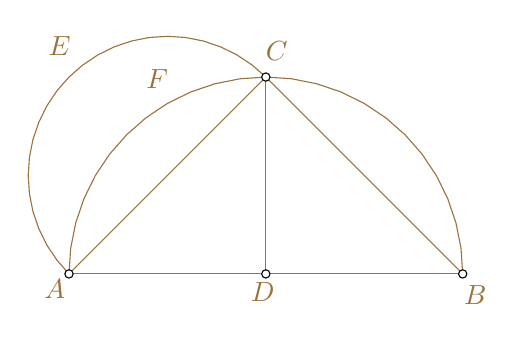
\begin{tikzpicture}
			\draw [shift={(2.5,0.)},lichsutoanhoc]  plot[domain=0.:3.141592653589793,variable=\t]({1.*2.5*cos(\t r)+0.*2.5*sin(\t r)},{0.*2.5*cos(\t r)+1.*2.5*sin(\t r)});
			\draw [lichsutoanhoc] (0.,0.)-- (5.,0.);
			\draw [shift={(1.25,1.25)},lichsutoanhoc]  plot[domain=0.7853981633974483:3.9269908169872414,variable=\t]({1.*1.7677669529663689*cos(\t r)+0.*1.7677669529663689*sin(\t r)},{0.*1.7677669529663689*cos(\t r)+1.*1.7677669529663689*sin(\t r)});
			\draw [lichsutoanhoc] (2.5,2.5)-- (0.,0.);
			\draw [lichsutoanhoc] (2.5,2.5)-- (5.,0.);
			\draw [lichsutoanhoc] (2.5,2.5)-- (2.5,0.);
				\draw [fill=white] (0.,0.) circle (1.5pt);
				\draw[color=lichsutoanhoc] (-0.18,-0.19) node {$A$};
				\draw [fill=white] (5.,0.) circle (1.5pt);
				\draw[color=lichsutoanhoc] (5.16,-0.27) node {$B$};
				\draw[color=lichsutoanhoc] (1.12,2.47) node {$F$};
				\draw [fill=white] (2.5,0.) circle (1.5pt);
				\draw[color=lichsutoanhoc] (2.46,-0.23) node {$D$};
				\draw [fill=white] (2.5,2.5) circle (1.5pt);
				\draw[color=lichsutoanhoc] (2.64,2.83) node {$C$};
				\draw[color=lichsutoanhoc] (-0.12,2.89) node {$E$};
		\end{tikzpicture}
		\caption{\small\textit{\color{lichsutoanhoc}Hình $1a$.}}
		\vspace*{-10pt}
	\end{figure}
	\setlength{\abovedisplayskip}{6pt}
	\setlength{\belowdisplayskip}{6pt}
	\textit{Chứng minh}. Nối $C$ với $D$. Ký hiệu, thí dụ, ${S_{\circletfillha ACB}}$  là diện tích nửa hình tròn $ACB$ đường kính $AB$. Vì $AB^2 = 2AC^2$  (Hình $1a$)  nên 
	\begin{align*}
		\frac{{{S_{\circletfillha ACB}}}}{{{S_{\circletfillha AEC}}}} = \frac{{\pi {{\left( {\frac{{AB}}{2}} \right)}^2}}/2}{{\pi {{\left( {\frac{{AC}}{2}} \right)}^2}}/2} = \frac{{A{B^2}}}{{A{C^2}}} = 2
	\end{align*}
	hay ${S_{\circletfillha ACB}} = 2{S_{\circletfillha AEC}}.$
	\vskip 0.05cm
	Nhưng  ${S_{\circletfillha ACB}} = {S_{\circletfillha ADC}} + {S_{\circletfillha BDC}} = 2{S_{\circletfillha ADC}}$ nên ${S_{\circletfillha AEC}} = {S_{\circletfillha ADC}}$.   Suy ra 
	\begin{align*}
		{S_{AECFA}} + {S_{AFCA}} = {S_{AECA}} = {S_{AFCA}} + {S_{\Delta ADC}}.
	\end{align*}
	Vậy diện tích hình trăng khuyết $AECFA$  bằng diện tích tam giác $ADC$,  hay trăng khuyết $AECFA$  đã được ``cầu phương".
	\vskip 0.05cm
	Một phiên bản khác của Định lý $1$ là
	\vskip 0.05cm
	\textbf{\color{lichsutoanhoc}Định lý} $\pmb{1'.}$ Dựng trên các cạnh của tam giác $ABC$ vuông ở $C$   các nửa đường tròn  đường kính $AB, AC, BC$. Khi ấy tổng diện tích hình trăng khuyết $L_1$  và $L_2$ bằng diện tích tam giác  $ABC$ (Hình $1b$).   
	\begin{figure}[H]
		\vspace*{-5pt}
		\centering
		\captionsetup{labelformat= empty, justification=centering}
		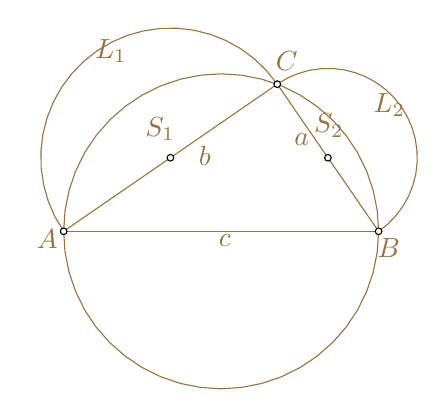
\begin{tikzpicture}[scale=0.8]
			\draw [shift={(2.5,0.)},lichsutoanhoc]  plot[domain=0.:3.141592653589793,variable=\t]({1.*2.5*cos(\t r)+0.*2.5*sin(\t r)},{0.*2.5*cos(\t r)+1.*2.5*sin(\t r)});
			\draw [lichsutoanhoc] (0.,0.)-- (5.,0.);
			\draw [lichsutoanhoc] (3.390811455834727,2.33590559529995)-- (0.,0.);
			\draw [lichsutoanhoc] (3.390811455834727,2.33590559529995)-- (5.,0.);
			\draw [shift={(1.6954057279173635,1.167952797649975)},lichsutoanhoc]  plot[domain=0.6032325047411791:3.744825158330972,variable=\t]({1.*2.058765241544895*cos(\t r)+0.*2.058765241544895*sin(\t r)},{0.*2.058765241544895*cos(\t r)+1.*2.058765241544895*sin(\t r)});
			\draw [shift={(4.195405727917364,1.167952797649975)},lichsutoanhoc]  plot[domain=-0.9675638220537177:2.1740288315360754,variable=\t]({1.*1.418268550101352*cos(\t r)+0.*1.418268550101352*sin(\t r)},{0.*1.418268550101352*cos(\t r)+1.*1.418268550101352*sin(\t r)});
			\draw [shift={(2.5,0.)},lichsutoanhoc]  plot[domain=-3.141592653589793:0.,variable=\t]({1.*2.5*cos(\t r)+0.*2.5*sin(\t r)},{0.*2.5*cos(\t r)+1.*2.5*sin(\t r)});
				\draw [fill=white] (0.,0.) circle (1.5pt);
				\draw[color=lichsutoanhoc] (-0.26,-0.13) node {$A$};
				\draw [fill=white] (5.,0.) circle (1.5pt);
				\draw[color=lichsutoanhoc] (5.16,-0.27) node {$B$};
				\draw[color=lichsutoanhoc] (2.56,-0.15) node {$c$};
				\draw [fill=white] (3.390811455834727,2.33590559529995) circle (1.5pt);
				\draw[color=lichsutoanhoc] (3.54,2.71) node {$C$};
				\draw[color=lichsutoanhoc] (2.24,1.19) node {$b$};
				\draw[color=lichsutoanhoc] (3.78,1.45) node {$a$};
				\draw [fill=white] (1.6954057279173635,1.167952797649975) circle (1.5pt);
				\draw[color=lichsutoanhoc] (1.53,1.62) node {$S_1$};
				\draw [fill=white] (4.195405727917364,1.167952797649975) circle (1.5pt);
				\draw[color=lichsutoanhoc] (4.21,1.68) node {$S_2$};
				\draw[color=lichsutoanhoc] (0.75,2.86) node {$L_1$};
				\draw[color=lichsutoanhoc] (5.17,2.) node {$L_2$};
		\end{tikzpicture}
		\caption{\small\textit{\color{lichsutoanhoc}Hình $1b$.}}
%		\vspace*{-5pt}
	\end{figure}
	\textit{Chứng minh}. Ta có   
	\begin{align*}
			{S_{\circletfillha AC}} + {S_{\circletfillha BC}} &= \frac{\pi}{2} {\left( {\frac{{AC}}{2}} \right)^2} + \frac{\pi}{2} {\left( {\frac{{BC}}{2}} \right)^2}\\
			&= \frac{\pi }{8}\left( {A{C^2} + B{C^2}} \right) \\
			&= \frac{\pi }{8}A{B^2} = {S_{\circletfillha ABC}}.
	\end{align*}
	Hay (Hình $1b$)
	\begin{align*}
		{S_{{L_1}}} + {S_{{S_1}}} + {S_{{L_2}}} + {S_{{S_2}}} = {S_{\Delta ABC}} + {S_{{S_1}}} + {S_{{S_2}}}.
	\end{align*}
	Suy ra
	\begin{align*}
		{S_{{L_1}}} + {S_{{L_2}}} = {S_{\Delta ABC}}.
	\end{align*}
	\textbf{\color{lichsutoanhoc}Định lý} $\pmb{2}.$ Diện tích nửa lục giác đều $CEFD$ bằng tổng diện tích nửa hình tròn $ALB$  và ba hình trăng khuyết $CGEMC$,  $EHFNE$, $FKDOF$ (Hình $2$).
	\begin{figure}[H]
		\vspace*{-10pt}
		\centering
		\captionsetup{labelformat= empty, justification=centering}
		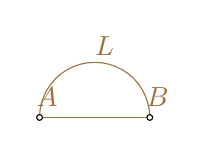
\begin{tikzpicture}[scale=0.7]
			\draw [lichsutoanhoc] (-5.,0.)-- (-3.,0.);
			\draw [shift={(-4.,0.)},lichsutoanhoc]  plot[domain=0.:3.141592653589793,variable=\t]({1.*1.*cos(\t r)+0.*1.*sin(\t r)},{0.*1.*cos(\t r)+1.*1.*sin(\t r)});
			
			\draw [fill=white] (-5.,0.) circle (1.5pt);
			\draw[color=lichsutoanhoc] (-4.86,0.37) node {$A$};
			\draw [fill=white] (-3.,0.) circle (1.5pt);
			\draw[color=lichsutoanhoc] (-2.86,0.37) node {$B$};
			
			\draw[color=lichsutoanhoc] (-3.82,1.29) node {$L$};
		\end{tikzpicture}
		\caption{\small\textit{\color{lichsutoanhoc}Hình $2a$.}}
		\vspace*{-10pt}
	\end{figure}
	\begin{figure}[H]
		\vspace*{-10pt}
		\centering
		\captionsetup{labelformat= empty, justification=centering}
		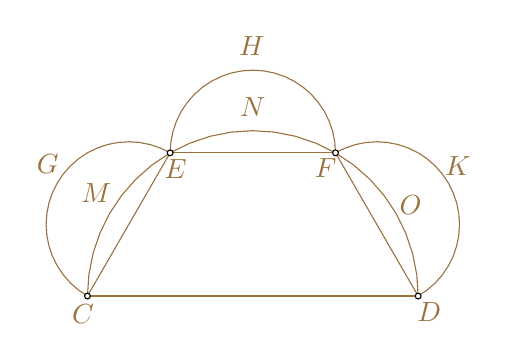
\begin{tikzpicture}[scale=0.7]
			\draw [lichsutoanhoc] (-1.,0.)-- (5.,0.);
			\draw [shift={(2.,0.)},lichsutoanhoc]  plot[domain=0.:3.141592653589793,variable=\t]({1.*3.*cos(\t r)+0.*3.*sin(\t r)},{0.*3.*cos(\t r)+1.*3.*sin(\t r)});
			\draw [shift={(-0.25,1.299038105676658)},lichsutoanhoc]  plot[domain=1.0471975511965979:4.188790204786391,variable=\t]({1.*1.5*cos(\t r)+0.*1.5*sin(\t r)},{0.*1.5*cos(\t r)+1.*1.5*sin(\t r)});
			\draw [shift={(2.,2.598076211353316)},lichsutoanhoc]  plot[domain=0.:3.141592653589793,variable=\t]({1.*1.5*cos(\t r)+0.*1.5*sin(\t r)},{0.*1.5*cos(\t r)+1.*1.5*sin(\t r)});
			\draw [shift={(4.25,1.299038105676658)},lichsutoanhoc]  plot[domain=-1.0471975511965983:2.0943951023931953,variable=\t]({1.*1.5*cos(\t r)+0.*1.5*sin(\t r)},{0.*1.5*cos(\t r)+1.*1.5*sin(\t r)});
			\draw [lichsutoanhoc] (-1.,0.)-- (0.5,2.598076211353316);
			\draw [lichsutoanhoc] (0.5,2.598076211353316)-- (3.5,2.598076211353316);
			\draw [lichsutoanhoc] (3.5,2.598076211353316)-- (5.,0.);
		
				\draw [fill=white] (-1.,0.) circle (1.5pt);
				\draw[color=lichsutoanhoc] (-1.08,-0.33) node {$C$};
				\draw [fill=white] (5.,0.) circle (1.5pt);
				\draw[color=lichsutoanhoc] (5.2,-0.29) node {$D$};
				\draw [fill=white] (0.5,2.598076211353316) circle (1.5pt);
				\draw[color=lichsutoanhoc] (0.6,2.31) node {$E$};
				\draw [fill=white] (3.5,2.598076211353316) circle (1.5pt);
				\draw[color=lichsutoanhoc] (3.32,2.33) node {$F$};
				\draw[color=lichsutoanhoc] (-1.72,2.39) node {$G$};
				\draw[color=lichsutoanhoc] (1.98,4.53) node {$H$};
				\draw[color=lichsutoanhoc] (5.72,2.35) node {$K$};
				\draw[color=lichsutoanhoc] (-0.84,1.87) node {$M$};
				\draw[color=lichsutoanhoc] (2.,3.43) node {$N$};
				\draw[color=lichsutoanhoc] (4.86,1.65) node {$O$};
		\end{tikzpicture}
		\caption{\small\textit{\color{lichsutoanhoc}Hình $2b$.}}
		\vspace*{-5pt}
	\end{figure}
	\textit{Chứng minh}. Dựng nửa hình tròn đường kính $AB = \dfrac{1}{2}CD$ (Hình $2a$). Dựng các nửa hình tròn đường kính $CE, EF, FD$ là ba cạnh liên tiếp của lục giác đều nội tiếp đường tròn đường kính  $CD$ (Hình $2b$). Vì 
	\begin{align*}
		C{D^2} = 4A{B^2} = A{B^2} + C{E^2} + E{F^2} + F{D^2}
	\end{align*}
	và tỷ lệ diện tích các hình tròn bằng tỷ lệ diện tích các hình vuông dựng trên đường kính của chúng nên 
	\begin{align*}
		&{S_{\circletfillha CEFD}} \\
		= &{S_{\circletfillha ALB}} + {S_{\circletfillha CGE}} + {S_{\circletfillha EHF}} + {S_{\circletfillha FKD}}.
	\end{align*}
	Trừ hai vế cho tổng diện tích ba hình viên phân $CMEC, ENFE, FODF$  ta được  
	\begin{align*}
		&{S_{CEFD}} \\
		= &{S_{\circletfillha ALB}} + {S_{CGEMC}} + {S_{EHFNE}} + {S_{FKDOF}}.
	\end{align*}
	Eudemus tin rằng Hippocrates đã chứng minh hai định lý trên, nhưng một chứng minh nghiêm túc vào thời điểm đó (khoảng năm $430$ trước Công nguyên) dường như khó có thể xảy ra. Chứng minh trong Quyển $12$ Chương $2$ \textit{Cơ sở} của Euclid dường như là của Eudoxus, một nhà toán học sống nửa thời gian giữa Hippocrates và Euclid. Tuy nhiên, hai cuốn sách đầu của Euclid dường như bắt nguồn từ Pythagoras, vì vậy sẽ có vẻ hợp lý khi giả định rằng công thức, ít nhất, phần lớn cuốn sách III và IV của \textit{Cơ sở}  là từ tác phẩm của Hippocrates. Hơn nữa, nếu Hippocrates đã đưa ra một chứng minh định lý về diện tích của các hình giới hạn bởi các hình tròn, thì Hippocrates chính là người phát minh ra phương pháp chứng minh gián tiếp trong toán học. 
	\vskip 0.05cm
	Từ các định lý về diện tích hình trăng khuyết, Hippocrates được coi là người đầu tiên trong lịch sử toán học tìm ra cách tính diện tích các hình cong (khác hình tròn). 
	\vskip 0.05cm
	Có cơ sở tương đối vững chắc về mặt lịch sử  khi nói rằng cầu phương hình tròn đã được phát triển bởi Hippocrates. Các học giả ngoài Simplicius cũng đề cập đến tác phẩm của Hippocrates. Simplicius sống ở thế kỷ VI, nhưng ông không chỉ trích dẫn Eudemus (khoảng năm $320$ TCN) mà còn dựa vào Alexander xứ Aphrodisias (khoảng năm $200$ CN), một trong những nhà bình luận chính về Aristotle. 
	Các kết quả trên dường như đã khuyến khích Hippocrates, cũng như những người cùng thời và những người kế nhiệm, ông hi vọng rằng cuối cùng hình tròn sẽ được cầu phương.
	\vskip 0.05cm
	Các kết quả của Hippocrates về cầu phương hình trăng khuyết có thể coi là những nỗ lực đáng kể của toán học vào thời điểm đó. Nó cho thấy rằng các nhà toán học Athens rất thành thạo trong việc xử lý các phép biến đổi diện tích và tỷ lệ.
	\vskip 0.05cm 
	Có ba quan điểm về những gì Hippocrates đã suy luận từ cầu phương hình trăng khuyết. Một số đã buộc tội ông vì tin rằng ông có thể cầu phương tất cả các hình trăng, trong đó có hình tròn; Những người khác nghĩ rằng ông biết những hạn chế công việc của mình, biết rằng nó được chứng minh chỉ với một số loại hình trăng. Một học giả lại viết rằng Hippocrates biết ông đã không cầu phương hình tròn nhưng cố đánh lừa đồng hương là mình đã thành công. 
	\vskip 0.05cm
	Hippocrates còn là người đầu tiên sử dụng ký hiệu chữ cái trong các hình hình học. Thật thú vị khi lưu ý rằng trong khi Hippocrates có đóng góp trong hai bài toán nổi tiếng, ông dường như đã không có tiến bộ trong bài toán chia ba một góc, một vấn đề được nghiên cứu phần nào sau đó bởi Hippias của Elis.
	\vskip 0.05cm
	\textbf{\color{lichsutoanhoc}Hippias xứ Elis}
	\vskip 0.05cm
	Vào cuối thế kỷ thứ năm TCN, một nhóm giáo viên chuyên nghiệp hoàn toàn không giống như người Pythagoras nổi lên mạnh mẽ ở Athens. Trong số này có Hippias, một người gốc Elis, đã sống tại Athens vào nửa sau của thế kỷ thứ năm TCN.  Ông là một trong những nhà toán học đầu tiên mà chúng ta có thông tin trực tiếp, vì chúng ta đọc được nhiều điều về ông từ \textit{Đối thoại} của Plato. Ông được cho là đã viết nhiều, từ toán học để diễn xướng, nhưng không có tác phẩm nào của ông còn tồn tại.  
	\vskip 0.05cm
	Hippias (khoảng $500-401$ TCN)  sống cùng thời với Socrates (khoảng $477-399$ TCN). Socrates được cho là đã mô tả Hippias đẹp trai, học giỏi nhưng khoe khoang và nông nổi. Trong \textit{Đối thoại} của Plato và \textit{Những kỷ vật} của Xenophon có những nhận xét không mấy hay ho về Hippias như một người tự coi mình là một chuyên gia trong mọi thứ từ lịch sử và văn học đến thủ công mỹ nghệ và khoa học. 
	\vskip 0.05cm
	Proclus và các nhà toán học khác đã gán tên trisectrix hoặc quadratrix cho Hippias, các đường cong khác đường tròn và đường thẳng. Điều này được mô tả như sau: Trong hình vuông $ABCD$ (Hình $3$), cho cạnh $AB$ di chuyển đều từ vị trí hiện tại của nó cho đến khi nó trùng với $DC$ và để chuyển động này diễn ra chính xác cùng thời gian $DA$ quay theo chiều kim đồng hồ từ vị trí hiện tại của nó cho đến khi nó trùng với $DC$.
	\begin{figure}[H]
		\vspace*{-10pt}
		\centering
		\captionsetup{labelformat= empty, justification=centering}
		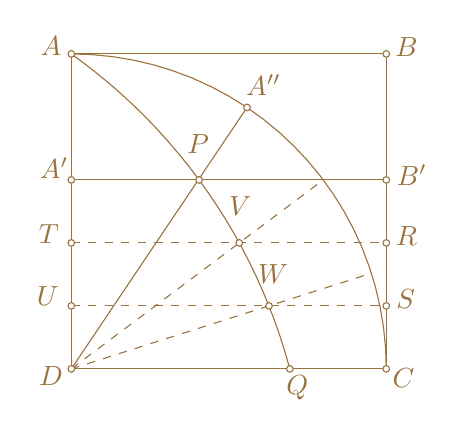
\begin{tikzpicture}[color=lichsutoanhoc,scale=0.8]
			\draw  (0,5)-- (5,5);
			\draw  (5,5)-- (5,0);
			\draw  (5,0)-- (0,0);
			\draw  (0,0)-- (0,5);
			\draw [dashed] (0,1)-- (5,1);
			\draw [dashed] (0,2)-- (5,2);
			\draw  (0,3)-- (5,3);
			\draw [shift={(0,0)}]  plot[domain=0:1.5707963267948966,variable=\t]({1*5*cos(\t r)+0*5*sin(\t r)},{0*5*cos(\t r)+1*5*sin(\t r)});
			\draw [dashed] (0,0)-- (4,3);
			\draw [dashed] (0,0)-- (4.763881899982941,1.5183640021466926);
			\draw  (0,0)-- (2.7888060926218334,4.1500072985183225);
			\draw [shift={(-5.217713374099582,-2.3231526288292588)}]  plot[domain=0.2613267271277395:0.9517332497157504,variable=\t]({1*8.991835034039855*cos(\t r)+0*8.991835034039855*sin(\t r)},{0*8.991835034039855*cos(\t r)+1*8.991835034039855*sin(\t r)});
			
			\draw[fill=white]  (0,0) circle (1.5pt);
			\draw (-0.3224250609980331,-0.10759386570245269) node {$D$};
			\draw[fill=white]  (0,5) circle (1.5pt);
			\draw (-0.3224250609980331,5.120007094122126) node {$A$};
			\draw[fill=white]  (5,5) circle (1.5pt);
			\draw (5.322715911592097,5.103305493611504) node {$B$};
			\draw[fill=white]  (5,0) circle (1.5pt);
			\draw (5.2726111100602315,-0.14099706672369602) node {$C$};
			\draw[fill=white]  (0,1) circle (1.5pt);
			\draw (-0.3725298625298981,1.1617277731047932) node {$U$};
			\draw[fill=white]  (5,1) circle (1.5pt);
			\draw (5.306014311081475,1.1116229715729282) node {$S$};
			\draw[fill=white]  (0,2) circle (1.5pt);
			\draw (-0.3558282620192764,2.1471222032314707) node {$T$};
			\draw[fill=white]  (5,2) circle (1.5pt);
			\draw (5.322715911592097,2.1137190022102277) node {$R$};
			\draw[fill=white]  (0,3) circle (1.5pt);
			\draw (-0.272320259466168,3.182621434890014) node {$A'$};
			\draw[fill=white]  (5,3) circle (1.5pt);
			\draw (5.406223914145205,3.082411831826284) node {$B'$};
			\draw[fill=white]  (2.7888060926218334,4.1500072985183225) circle (1.5pt);
			\draw (3.051298242147547,4.502047875229125) node {$A''$};
			\draw[fill=white]  (3.1375097758163863,1) circle (1.5pt);
			\draw (3.201612646743142,1.512461383827848) node {$W$};
			\draw[fill=white]  (2.6666666666666665,2) circle (1.5pt);
			\draw (2.68386303091387,2.581363816507634) node {$V$};
			\draw[fill=white]  (3.4688313441730543,0) circle (1.5pt);
			\draw (3.5857494584874408,-0.2927680433) node {$Q$};
			\draw[fill=white]  (2.029157907327644,3) circle (1.5pt);
			\draw (2.015799010489003,3.5667582466343117) node {$P$};
		\end{tikzpicture}
		\caption{\small\textit{\color{lichsutoanhoc}Hình $3$.}}
		\vspace*{-15pt}
	\end{figure}
	Nếu vị trí của hai đường chuyển động tại bất kỳ thời gian tương ứng được cho bởi $A'B'$ và $DA''$, và nếu $P$ là giao điểm của $A'B'$ và $DA''$, quỹ tích của $P$ trong quá trình chuyển động sẽ là trisectrix của Hippias -- đường cong $APQ$ trong Hình $3$. Với đường cong này, việc cắt bỏ một góc được thực hiện một cách dễ dàng. Ví dụ: nếu $PDC$ là góc được cắt bỏ, người ta chỉ cần cắt các đoạn $B'C$ và $A'D$ làm ba phần tại các điểm $R$, $S$, $T$ và $U$. Nếu đường $TR$ và $US$ cắt trisectrix ở $V$ và $W$, tương ứng, các dòng $VD$ và $WD$, theo thuộc tính của trisectrix, chia góc $PDC$ thành ba phần bằng nhau. Đường cong Hippias thường được gọi là quadratrix, vì nó có thể được sử dụng để cầu phương hình tròn. Người ta đã phỏng đoán rằng Hippias biết về phương pháp cầu phương này nhưng cầu phương qua đường cong Hippias do Dinostratus đưa ra sau này.
	\vskip 0.05cm
	Về tính cách, Plato đối lập Hippias với Socrates, người ta có thể tạo ra nhiều sự tương phản giống nhau bằng cách so sánh Hippias với một người cùng thời khác--nhà toán học thuộc trường phái Pythagoras là Archytas xứ Tarentum.
	\vskip 0.05cm
	\textbf{\color{lichsutoanhoc}Philolaus và Archytas xứ Tarentum}
	\begin{figure}[H]
		\vspace*{-5pt}
		\centering
		\captionsetup{labelformat= empty, justification=centering}
		\includegraphics[width= 0.65\linewidth]{2}
		\caption{\small\textit{\color{lichsutoanhoc}Archytas ($428-347$ TCN).}}
		\vspace*{-10pt}
	\end{figure}
	Pythagoras được cho là đã lui về Metapontum vào cuối đời và đã chết ở đó khoảng năm $500$ TCN.  Ông không để lại các tác phẩm viết, nhưng ý tưởng của ông đã được thực hiện bởi một số lượng lớn đệ tử. Trung tâm ở Croton đã bị bỏ hoang khi một nhóm đối thủ chính trị từ Sybaris đã bất ngờ sát hại nhiều thủ lĩnh, nhưng những người thoát khỏi vụ thảm sát đã mang theo các học thuyết của trường phái Pythagoras đến các khu vực khác của thế giới Hy Lạp. Trong số những người học được từ những người tị nạn Pythagoras có Philolaus xứ Tarentum. Ông được cho là đã viết bài tường thuật đầu tiên về thuyết Pythagoras.  Rõ ràng, đây là cuốn sách mà từ đó Plato rút ra kiến thức của ông về Pythagoras.  
	\vskip 0.05cm
	Sự cuồng tín số rất đặc trưng của Pythagoras hiển nhiên đã được chia sẻ bởi Philolaus. Ông giải thích phần lớn những truyền thuyết huyền bí cũng như kiến thức về vũ trụ học của Pythagoras. Các sơ đồ vũ trụ của Philolaus được cho là đã được sửa đổi bởi hai người thuộc trường phái Pythagoras, Ecphantus và Hicetas, những người đã giải thích ngày và đêm bằng cách đặt trái đất quay.  
	\vskip 0.05cm
	Sự cực đoan của việc tôn thờ số của Philolaus dường như cũng đã trải qua một số sửa đổi, đặc biệt hơn là dưới bàn tay của Archytas, một học trò của Philolaus xứ Tarentum. 
	\vskip 0.05cm
	Archytas tin tưởng chắc chắn vào hiệu quả của số. Trong nhiều năm liên tiếp, ông được bầu làm tướng, và ông chưa bao giờ bị đánh bại. Ông tốt bụng và là một người yêu trẻ em, vì ông là được cho là đã phát minh ra ``Archytas’s rattle", một đồ chơi bằng gỗ, được chế tạo để làm thú vui cho trẻ. Archytas tiếp tục truyền thống Pythagoras trong việc đặt số học lên trên hình học, nhưng sự nhiệt tình của ông đối với con số nhẹ hơn ở Philolaus.  Ông đã viết ứng dụng của số học, hình học đối với âm nhạc, và có thể là Philolaus hoặc Archytas đã đưa ra khái niệm ``trung bình điều hòa". 
	\vskip 0.05cm
	Archytas đã chú ý nhiều đến âm nhạc nhiều hơn so với những người tiền nhiệm của mình và ông cảm thấy rằng môn học này phải đóng một vai trò lớn hơn văn học trong việc giáo dục trẻ em. Archytas dường như đã chú ý đáng kể đến vai trò của toán học trong chương trình giảng dạy, và ông được coi là đã chỉ định bốn nhánh trong tứ giác toán học -- số học (hoặc số còn lại), hình học (hoặc độ lớn khi dừng lại), âm nhạc (hoặc các con số đang chuyển động) và thiên văn học (hoặc độ lớn trong chuyển động). Các môn học này, cùng với bộ ba bao gồm ngữ pháp, tu từ và biện chứng (mà Aristotle bắt nguồn từ Zeno), sau này tạo thành bảy nghệ thuật tự do; vì thế Archytas được coi là có đóng góp nổi bật đưa vai trò của toán học lên một vị trí quan trọng trong giáo dục. 
	\vskip 0.05cm
	Tuy nhiên, đóng góp quan trọng nhất của Archytas cho toán học có thể là sự can thiệp của ông với bạo chúa Dionysius để cứu sống người bạn Plato của mình. Plato cho đến cuối cuộc đời vẫn cam kết sâu sắc với sự tôn kính Pythagoras về số và hình học, và vị thế tối cao của Athens trong thế giới toán học của thế kỷ thứ tư TCN là kết quả chủ yếu từ sự nhiệt tình của Plato, ``nhà tạo ra các nhà toán học." 
	\begin{figure}[H]
		\vspace*{-5pt}
		\centering
		\captionsetup{labelformat= empty, justification=centering}
		\includegraphics[width= 0.65\linewidth]{4}
		\caption{\small\textit{\color{lichsutoanhoc}Plato ($428-347$ TCN).}}
		\vspace*{-10pt}
	\end{figure}
	\textbf{\color{lichsutoanhoc}Menaechmus}
	\vskip 0.05cm
	Eudoxus được ghi nhớ trong lịch sử toán học không chỉ vì công việc của riêng mình mà còn thông qua học sinh của mình. 
	\vskip 0.05cm
	Ở Hy Lạp, có một sợi dây tiếp nối truyền thống từ thầy sang trò.  Thí dụ, Plato học được từ Archytas, Theodorus và Theaetetus; ảnh hưởng của Plato lần lượt được truyền qua Eudoxus cho anh em Menaechmus và Dinostratus, cả hai đều đạt được thành tựu xuất sắc trong toán học. 
	\vskip 0.05cm
	Menaechmus nổi tiếng là người đã khám phá ra các đường cong mà sau này được gọi là hình elip, parabol và hyperbol, các thiết diện được cắt ra bởi hình nón (các đường cong conic).
	\vskip 0.05cm
	Menaechmus đã thành công dựa trên các đường cong conic với các tính chất thích hợp để giải bài toán gấp đôi khối lập phương. 
	\vskip 0.05cm
	Proclus đã viết rằng Menaechmus là một trong những người đã ``làm cho toàn bộ hình học trở lên hoàn hảo hơn" (made the whole of geometry more perfect). Chúng ta biết rằng Menaechmus đã dạy Alexander Đại đế, và huyền thoại nổi tiếng thuộc về Menaechmus, khi học trò của ông yêu cầu một lối tắt đến hình học: ``Hỡi Vua, để đi qua đất nước, có những con đường hoàng gia và những con đường dành cho công dân chung; nhưng trong hình học, chỉ có một con đường cho tất cả mọi người".
	\begin{figure}[H]
		\vspace*{-5pt}
		\centering
		\captionsetup{labelformat= empty, justification=centering}
		\includegraphics[width= 0.65\linewidth]{3}
		\caption{\small\textit{\color{lichsutoanhoc}Menaechmus ($380-320$ TCN).}}
		\vspace*{-10pt}
	\end{figure}
	Chứng cứ Menaechmus phát hiện ra các thiết diện conic là do một lá thư từ Eratosthenes đến Vua Ptolemy Euergetes, được Eutocius trích dẫn khoảng $700$ năm sau đó, trong đó bài toán gấp đôi khối lập phương được đề cập. 
	\vskip 0.05cm
	\textbf{\color{lichsutoanhoc}Dinostratus và cầu phương hình tròn}
	\vskip 0.05cm
	Dinostratus, anh trai của Menaechmus, cũng là một nhà toán học; một người đã ``giải quyết" bài toán gấp đôi thể tích khối lập phương, người còn lại ``giải quyết" bài toán cầu phương hình tròn. 
	\vskip 0.05cm
	\textbf{\color{lichsutoanhoc}Thay lời kết}
	\vskip 0.05cm
	Tất nhiên, người Hy Lạp cũng hiểu rằng việc sử dụng đường cong trong các bài toán chia ba góc và các bài toán cầu phương đã vi phạm quy tắc của trò chơi -- chỉ cho phép sử dụng compa và thước thẳng. ``Lời giải" của Hippias, Menaechmus và Dinostratus, như các tác giả của chúng cũng nhận ra, là ngụy tạo; vì thế, việc tìm kiếm các giải pháp khác, chính tắc hoặc bất hợp pháp, tiếp tục, với kết quả là một số đường cong mới đã được phát hiện bởi các nhà hình học Hy Lạp.
	\vskip 0.05cm
	\textbf{\color{lichsutoanhoc}Tài liệu tham khảo chính}
	\vskip 0.05cm
	[$1$] David M. Burton, \textit{The History of Mathematics, An Introduction, Seventh Edition}, McGraw--Hill, $2011$. Chapter $3$: The Beginnings of Greek Mathematics, pp. $116-139$.
	\vskip 0.05cm
	[$2$] Thomas Heath, \textit{A History of Greek Mathematics, Oxford at the Clarendon Press}, $1921$, Volume $1$: From Thales to Euclid, pp. $170-353$.
	\vskip 0.05cm   
	[$3$] Victor J. Katz, \textit{A History of Mathematics, An Introduction}, Third Edition, Addison--Wesley, $2009$. Chapter $2$: \textit{The Beginnings of Mathematics in Greek}, pp. $40-49$.
	\vskip 0.05cm
	[$4$] Uta C. Merzbach and Carl B. Boyer, \textit{A
	History of Mathematics}, Third Edition, John Wiley \& Sons, $2011$, pp. $57-89$.
	\vskip 0.05cm
	[$5$] Ngô Việt Trung, \textit{Lý thuyết Galois về các vấn đề giải phương trình bằng căn thức, dựng hình bằng thước kẻ và compa}, Nhà xuất bản Đại học Quốc gia Hà Nội, $2006$.
	\vskip 0.05cm
	\textbf{\color{lichsutoanhoc}Tài liệu tham khảo}
	\vskip 0.05cm 
	[$6$] George Johston Allman, \textit{Greek Geometry: From Thales to Euclid}, Dublin Universty Press, $1877$, pp. $432$.  
	\vskip 0.05cm
	[$7$] Euclid, \textit{Cơ sở của Hình học}, Nhà xuất bản Trí thức, $2016$, pp. $350$.
	\vskip 0.05cm
	[$8$] R. Lloyd, \textit{Early Greek Science: Thales to Aristotle}, $1970$, Chatto \& Windus, London, pp. $156$. 
	\vskip 0.05cm
	[$8$] Nicomachus of Gerasa, \textit{Introduction to Arithmetic}, Translated into English by Martin Luther D’ooge, The Macmillan Company, New York, $1926$.
	\vskip 0.05cm
	[$9$] Proclus, \textit{Commentaries on Euclid’s books}, Vol. $1$, pp. $330$.
	\vskip 0.05cm
	[$10$] Arpad Szabo, \textit{The beginnings of Greek Mathematics}, Springer, $1978$, pp. $363$.
	\vskip 0.05cm
	[$11$] M. L. West, \textit{Early Greek Philosophy and the Orient}, Oxford at the Clarendon Press, $1971$, pp. $255$.
\end{multicols}

	 \newpage

	 \setcounter{figure}{0}
	 \thispagestyle{timhieukhoahocnone}
\pagestyle{timhieukhoahoc}
\everymath{\color{timhieukhoahoc}}
\blfootnote{$^1$\text{\color{timhieukhoahoc}Viện Sinh thái và Môi trường Đông Dương.}}
\graphicspath{{../timhieukhoahoc/pic/}}
\begingroup
\AddToShipoutPicture*{\put(0,616){\includegraphics[width=19.3cm]{../bannertimhieu}}}
\AddToShipoutPicture*{\put(108,522){\includegraphics[scale=1]{../tieude.pdf}}}
\centering
\endgroup
\vspace*{185pt}

\begin{multicols}{2}
	Nhắc đến Mendel, người ta thường nghĩ đến các bài tập về di truyền liên quan đến tổ hợp và xác suất trong môn sinh học. Tuy nhiên, bối cảnh lịch sử cũng như sự liên hệ của các định luật Mendel với các vấn đề khác trong sinh học lại thường ít được các tài liệu chú trọng giới thiệu. Nhân dịp kỷ niệm $200$ năm ngày sinh Mendel ($20/07/1822$ -- $20/07/2022$), chúng ta hãy cùng tìm hiểu về thí nghiệm lai giống đậu kinh điển của ông, vai trò của thống kê và tổ hợp trong thí nghiệm này cùng một số vấn đề xung quanh sự ra đời của di truyền học.
	\begin{figure}[H]
		\centering
		\vspace*{-5pt}
		\captionsetup{labelformat= empty, justification=centering}
		\includegraphics[width=1\linewidth]{image011}
		\vspace*{-15pt}
	\end{figure}
	$\pmb{1.}$ \textbf{\color{timhieukhoahoc}Giai đoạn ban đầu}
	\vskip 0.1cm
	Johann Mendel sinh năm $1822$ tại Heizendorf, vùng Silesia, thuộc đế quốc Áo (ngày nay thuộc cộng hòa Czech). Ông được gia đình cho đi học đến năm $21$ tuổi nhưng do hoàn cảnh tài chính, ông lựa chọn trở thành tu sỹ ở một tu viện ở Brno và đổi tên thành Gregor.
	\vskip 0.1cm
	Sau một thời gian, ông được tu viện phân công dạy khoa học tự nhiên tại trường học của nhà thờ ở Znojmo, một địa phương gần đó. Công việc này cũng phù hợp với sự yêu thích khoa học sẵn có của Mendel. 
	\vskip 0.1cm
	Đến năm $1849$, chính phủ Áo yêu cầu tất cả các giáo viên cần phải trải qua kỳ thi để cấp chứng chỉ hành nghề. Tuy Mendel không vượt qua được kỳ thi khảo sát do Đại học Vienna tổ chức, ông vẫn đủ tiêu chuẩn để được theo học tại đây dưới dạng sinh viên dự thính.Trong giai đoạn từ $1851$ đến $1853$, Mendel theo học nhiều môn khác nhau: vật lý, hóa học, toán học, động vật học, thực vật học và cổ sinh học. Trong quá trình đó, ông được tiếp cận với các bài giảng của Franz Unger, một nhà thực vật học nổi tiếng lúc đó. Dựa trên các nghiên cứu về hóa thạch cổ đại cùng những kiến thức mới về tế bào và sự phát triển phôi ở thực vật, Unger đưa ra một mô hình về sự tiến hóa của sinh vật: theo đó, một loài không tự nhiên sinh ra mà là hậu duệ của một loài trước đó và sự tiến hóa không tiến hành theo dạng tuyến tính mà có dạng hình cây. Unger chịu nhiều chỉ trích từ các nhân vật bảo thủ do quan điểm này ngược với các giải thích dựa trên tôn giáo. Dù bản thân là một thành viên của nhà thờ, Mendel vẫn tham gia học ở lớp của Unger.
	\vskip 0.1cm
	Tháng $8$ năm $1853$, Mendel trở lại tu viện ở Brno. Môi trường ở đây vẫn luôn chịu sự kiểm duyệt của giáo hội với các cuộc thanh tra, trong đó Mendel bị nhận định là dạng cá biệt, chuyên nghiên cứu ``các khoa học vớ vẩn". Năm $1856$, Mendel trở lại Vienna để tham dự kỳ thi sát hạch giáo viên lần thứ hai. Tuy nhiên, ông bị ốm nặng sau câu hỏi đầu tiên và phải trở về nằm giường ở Brno một thời gian. Dù mong muốn trở thành giáo viên dạy khoa học bị tan vỡ, Mendel vẫn không từ bỏ và tiến hành một thí nghiệm mà ông đã ấp ủ từ trong vài năm trước.
	\begin{figure}[H]
		\centering
		\vspace*{-5pt}
		\captionsetup{labelformat= empty, justification=centering}
		\includegraphics[width=1\linewidth]{image002}
		\caption{\small\textit{\color{timhieukhoahoc}Hình $1$. Loài đậu Pisum sativum.}}
		\vspace*{-10pt}
	\end{figure}
	Mendel tiến hành thí nghiệm để tìm hiểu các vấn đề về sự lai giống của sinh vật, một chủ đề ông được tiếp xúc trong quá trình học ở Đại học Vienna. Đối tượng của ông là loài đậu \textit{Pisum sativum}, với các dòng thuần đã được Mendel chọn lọc trong vòng hai năm trước~đó.
	\vskip 0.1cm
	$\pmb{2.}$ \textbf{\color{timhieukhoahoc}Thí nghiệm trên cây đậu}
	\vskip 0.1cm
	Quá trình thí nghiệm của Mendel được tiến hành trong suốt $8$ năm từ $1856$ đến $1863$. Trong các giống đậu đã nhân được, ông chọn ra $22$ giống để tiến hành thí nghiệm. Chúng đã được kiểm chứng là dòng thuần. Mendel sử dụng $7$ đặc điểm để phân biệt chúng, mỗi đặc điểm có hai dạng khác nhau. Các đặc điểm về hạt (màu sắc và bề mặt) có thể được quan sát trực tiếp trên các hạt đậu. Các đặc điểm còn lại yêu cầu việc gieo hạt và quan sát cây trưởng thành.
	\vskip 0.1cm
	$\pmb{2.1}$ \textbf{\color{timhieukhoahoc}Tỷ lệ trong lai giống}
	\vskip 0.1cm
	Đầu tiên, Mendel tiến hành lai các dòng thuần (F$0$) với nhau để cho ra thế hệ lai F$1$. Kết quả cho thấy với mỗi một đặc điểm, sẽ có một dạng trội mà tất cả các F$1$ đều biểu hiện theo dạng này, dạng còn lại trở thành dạng lặn. Tiếp theo, Mendel cho các F$1$ tự thụ phấn để sinh ra các F$2$. Kết quả thống kê cho thấy tỷ lệ trội~:~lặn ở F2 gần với tỷ lệ $3$~:~$1$ cho cả $7$ đặc điểm. Đặc biệt, khi cho hạt của cùng một cây F$1$ hoặc trong cùng một quả mọc lên, dạng trội và dạng lặn đều có thể xuất hiện.
	\vskip 0.1cm
	Mendel lại tiếp tục cho các cây F$2$ tự thụ phấn để cho ra thế hệ F$3$. Ông nhận thấy rằng các F$2$ mang đặc điểm lặn cho ra thế hệ F$3$ giống như vậy. Trong các cây F$2$ mang đặc điểm trội, $2/3$ trong số chúng có F$3$ theo tỷ lệ trội~:~lặn là $3$~:~$1$, giống với khi lai hai dòng thuần; còn $1/3$ còn lại cho F$3$ toàn bộ trội (các tỷ lệ này đã được làm tròn từ dữ liệu thống kê). Từ kết quả này, Mendel nhận thấy khi lai các cây lai F$1$, một nửa các hạt thu được (F$2$) sẽ là dạng lai giống như F$1$ còn một nửa còn lại trở thành dòng thuần trội hoặc dòng thuần lặn (giống F$0$) với số lượng như nhau.
	\vskip 0.1cm
	Ông tiến hành lặp lại các thí nghiệm trên các đặc điểm của hạt đậu cho $6$ thế hệ và trên các đặc điểm của cây đậu cho $4$ thế hệ liên tiếp. Kết quả cho cả $7$ đặc điểm khẳng định rằng thế hệ sau của các cây lai từ hai dòng thuần được phân chia theo tỷ lệ $2$~:~$1$~:~$1$ cho dạng lai và hai dạng thuần.
	\vskip 0.1cm
	Mendel ký hiệu $A$ là dạng trội, $a$ là dạng lặn và $Aa$ là dạng lai kết hợp của hai dạng thuần (Tất nhiên là lúc đó Mendel không thể biết được việc vật liệu di truyền có hai bản sao theo cặp. Theo cách ký hiệu ngày nay, các ký hiệu trên phải là $AA$, $aa$ và $Aa$). Ông biểu diễn thế hệ F$2$ theo biểu thức: $A + 2Aa + a$.
	\begin{figure}[H]
		\centering
		\vspace*{-5pt}
		\captionsetup{labelformat= empty, justification=centering}
		\includegraphics[width=1\linewidth]{image003}
		\caption{\small\textit{\color{timhieukhoahoc}Hình $2$. Các đặc điểm Mendel nghiên cứu trong thí nghiệm lai cùng tỷ lệ trội~:~lặn quan sát được.}}
		\vspace*{-10pt}
	\end{figure}
	$\pmb{2.2}$ \textbf{\color{timhieukhoahoc}Lai nhiều đặc điểm}
	\vskip 0.1cm
	Mendel lại tiếp tục tiến hành thí nghiệm về sự tương tác giữa nhiều hơn một đặc điểm khác nhau khi lai. Trong thí nghiệm cho hai đặc điểm, Mendel lai dòng thuần hạt tròn $(A)$ -- hạt vàng $(B)$ với dòng thuần hạt nhăn $(a)$ -- hạt xanh $(b)$. Ở đây, các chữ cái in biểu diễn dạng trội còn các chữ cái thường biểu diễn dạng lặn của một đặc điểm. Kết quả cho F$1$ toàn bộ có hạt tròn và vàng. Khi cho $15$ cây F$1$ tự thụ phấn, Mendel thu được $556$ hạt F$2$. Các F$2$ này được trồng thành cây và đặc điểm của các hạt của chúng (tức F$3$) được thống kê để phân loại F$2$.
	\begin{table}[H]
		\vspace*{-5pt}
		\centering
		\captionsetup{labelformat= empty, justification=centering}
		\resizebox{\columnwidth}{!}{\begin{tabular}{|l|p{1.6cm}|p{2cm}|p{1.6cm}|}
			\hline
			&$A$&	$Aa$&	$A$\\
			\hline
			$B$&	$AB$ (tròn vàng)~:~$38$&	$AaB$ (tròn vàng + nhăn vàng)~:~$60$&	$aB$ (nhăn vàng)~:~$28$\\
			\hline
			$Bb$&	$ABb$ (tròn vàng + tròn xanh)~:~$65$&	$AaBb$ (tròn vàng + tròn xanh + nhăn vàng + nhăn xanh)~:~$138$&	$aBb$ (nhăn vàng và nhăn xanh)~:~$68$\\
			\hline
			$b$&	$Ab$ (tròn xanh)~:~$35$& $Aab$ (tròn xanh + nhăn xanh)~:~$67$&	$ab$ (nhăn xanh)~:~$30$\\
			\hline
		\end{tabular}}
		\caption{\small\textit{\color{timhieukhoahoc}Bảng $1$. Kết quả phân loại $556$ cây F$2$ dựa trên hạt của chúng.}}
		\vspace*{-10pt}
	\end{table}
	Mendel phân loại các dạng thu được thành ba nhóm: nhóm có cả hai đặc điểm đều là thuần ($AB$, $Ab$, $aB$ và $ab$), nhóm có một đặc điểm thuần và một đặc điểm lai ($ABb$, $aBb$, $AaB$, $Aab$) và nhóm có cả hai đặc điểm là lai ($AaBb$). Ông nhận định rằng số liệu của các dạng này: $32$, $65$, $138$ gần với bộ số $33$, $66$, $132$ ứng với tỷ lệ $1 : 2 : 4$. Có thể thấy trực giác phân tích số liệu của Mendel rất tốt. Ông kết luận rằng hiện tượng quan sát được là do sự kết hợp của hai biểu thức $A + 2Aa + a$ và $B + 2Bb +b$. Thật vậy, tiến hành phép nhân hai biểu thức này, ta được:
	\begin{align*}
		&AB + 2AaB + aB + 2ABb +4AaBb\\
		&+ 2aBb + Ab + 2Aab + ab
	\end{align*}
	Tương tự, khi tiến hành thí nghiệm lai cho ba đặc điểm, kết quả phân bố cũng phù hợp với tích của ba biểu thức $A + 2Aa + a$, $B + 2Bb +b$ và $C + 2Cc + c$.
	\vskip 0.1cm
	Một điểm tương đối thú vị ở đây là Mendel không sử dụng công thức nhân xác suất như ngày nay ta vẫn dùng khi giải các bài toán tổ hợp trong di truyền mà biểu diễn số lượng các nhóm trong mỗi đặc điểm theo biểu thức đại số với các hệ số có tỷ lệ ứng với số lượng từng nhóm rồi tiến hành nhân các biểu thức đại số để cho ra tỷ lệ giữa các nhóm tổ hợp.
	\vskip 0.1cm
	Các kết quả của hai thí nghiệm này (cũng như nhiều thí nghiệm tương tự cho các bộ đặc điểm khác) cho phép Mendel kết luận rằng việc di truyền các đặc điểm mà ông nghiên cứu là độc lập.
	\vskip 0.1cm
	$\pmb{2.3}$ \textbf{\color{timhieukhoahoc}Thí nghiệm về tế bào sinh sản}
	\vskip 0.1cm
	Trong các thí nghiệm trước, khi tiến hành lai các F$0$, Mendel đem phấn từ các cây dòng thuần lặn đến thụ phấn cho hoa của các cây dòng thuần trội. Câu hỏi đặt ra là nếu vai trò hoa/phấn hoa được đảo lại thì kết quả có vẫn luôn vậy không? Ông giả định rằng số loại tế bào noãn/phấn hoa được tạo ra bằng với số lượng các dạng tổ hợp của các dòng thuần (ví dụ $AB$, $Ab$, $aB$, $ab$ cho trường hợp hai đặc điểm). Đồng thời khi kết hợp giả định này với việc tỷ lệ của mỗi tổ hợp so với tổng số là giống nhau, Mendel hy vọng nó có thể giải thích các kết quả về phân bố tổ hợp của các đặc điểm ở những thí nghiệm trước đó.
	\vskip 0.1cm
	Đầu tiên Mendel thụ phấn cho hoa của F$0$ trội $AB$ bằng phấn từ cây F$0$ lặn $ab$ để thu được dạng lai $AaBb$. Tiếp đó, ông tiến hành $4$ quá trình thụ phấn:
	\vskip 0.1cm
	$\bullet$ cho hoa của dạng lai từ phấn hoa của $AB$
	\vskip 0.1cm
	$\bullet$ cho hoa của dạng lai từ phấn hoa của $ab$
	\vskip 0.1cm
	$\bullet$ cho hoa của $AB$ từ phấn hoa của dạng lai
	\vskip 0.1cm
	$\bullet$ cho hoa của ab từ phấn hoa của dạng lai
	\vskip 0.1cm
	Với mỗi thí nghiệm, tất cả hoa của một cây đều được thụ phấn. Mendel nhận định rằng nếu giả định của mình là đúng thì các cây lai sẽ có các tế bào noãn và tế bào phấn hoa của các dạng $AB$, $Ab$, $aB$, và $ab$. Khi chúng kết hợp với các tế bào noãn và tế bào phấn hoa từ các cây bố mẹ $AB$ và $ab$ thì sẽ có các mẫu lần lượt như sau trong từng trường hợp:
	\vskip 0.1cm
	$\bullet$ $AB$, $ABb$, $AaB$, $AaBb$
	\vskip 0.1cm
	$\bullet$ $AaBb$, $Aab$, $aBb$, $ab$
	\vskip 0.1cm
	$\bullet$ $AB$, $ABb$, $AaB$, $AaBb$
	\vskip 0.1cm
	$\bullet$ $AaBb$, $Aab$, $aBb$, $ab$
	\vskip 0.1cm
	và trong mỗi trường hợp, các dạng đều xuất hiện với tần số như nhau.
	\vskip 0.1cm
	Mendel nhận thấy kết quả thí nghiệm không phụ thuộc vào việc phấn hoa được lấy từ dòng thuần nào khi tiến hành lai F$0$. Tất nhiên, ông cũng chỉ ra rằng số liệu thống kê từ thí nghiệm không thể hoàn toàn khớp một cách chính xác như công thức toán học.
	\vskip 0.1cm
	Tiếp theo Mendel tiến hành lai một cách phức tạp hơn. Đầu tiên, ông dùng phấn hoa của $ab$ để thụ phấn cho $Ab$ để tạo dạng lai $Aab$ (ký hiệu $A$~:~hoa vàng, $a$~:~hoa trắng; $B$~:~thân dài, $b$~:~thân ngắn). Đồng thời, ông cũng dùng phấn hoa này của $ab$ để thụ phấn cho $aB$ cho ra dạng lai $aBb$. Sau đó, phấn hoa của $aBb$ được dùng để thụ phấn cho $Aab$ để cho ra các tổ hợp $AaBb$, $aBb$, $Aab$ và $ab$. Sau khi gieo hạt và quan sát, tỷ lệ $Aa$~:~$a$ và $Bb$~:~$b$ đều gần với $1$~:~$1$.
	\vskip 0.1cm
	Các kết quả trên cùng những thí nghiệm tương tự với các đặc điểm khác cho Mendel kết luận rằng ở tế bào noãn hay tế bào phấn hoa của cây lai thì tỷ lệ cho mỗi tổ hợp từ các dạng thuần là như nhau. Chẳng hạn, cây lai $AaB$ sẽ có số lượng các tế bào sinh sản với tỷ lệ $AB$~:~$aB$ gần với $1$~:~$1$. Còn cây lai $AaBb$ sẽ có tỷ lệ $AB$~:~$Ab$~:~$aB$~:~$Bb$ gần với $1$~:~$1$~:~$1$~:~$1$.
	\vskip 0.1cm
	$\pmb{3.}$ \textbf{\color{timhieukhoahoc}Sự ra đời của di truyền học}
	\vskip 0.1cm
	Mendel trình bày kết quả thí nghiệm trong suốt $8$ năm của mình ở Hội lịch sử tự nhiên Brno vào năm $1865$ và công bố bài báo về nghiên cứu này vào năm $1866$. Tuy nhiên, nó hầu như không được chú ý đến cho đến tận vài thập kỷ sau.
	\vskip 0.1cm
	Về mặt lịch sử, trong giai đoạn nửa cuối thế kỷ $19$, bản chất của sự tiến hóa của sinh vật trở thành một vấn đề nổi bật. Darwin trong cuốn sách ``Nguồn gốc các loài" năm $1859$ đề xuất thuyết tiến hóa của mình mà theo đó sự tiến hóa là một quá trình liên tục thông qua chọn lọc tự nhiên: các cá thể với các tính trạng thích nghi với điều kiện môi trường sẽ có lợi thế hơn để sống sót và sinh sản, chúng di truyền lại các tính trạng này cho hậu duệ và theo thời gian các tính trạng có ưu thế sẽ phổ biến hơn trong quần thể. Theo Darwin, quá trình này có thể dẫn đến sự tạo thành loài mới khi các quần thể của cùng một loài thích nghi với các điều kiện sống khác nhau dẫn tới sự phân hóa.
	\vskip 0.1cm
	Đồng thời, Darwin cũng đưa ra giả thuyết của mình về di truyền. Theo đó, các tế bào trong cơ thể của sinh vật sẽ sinh ra các thành phần gọi là ``gemmule". Chúng sẽ tích tụ trong tế bào sinh sản và do đó được truyền cho thế hệ sau. Việc lai giống dẫn đến sự trộn lẫn gemmule. Có những dạng gemmule sẽ trội hơn, lấn át các dạng khác. Cường độ của các dạng gemmule có thể thay đổi theo từng thế hệ và có những trường hợp biểu hiện ra các gemmule dạng lặn. Giả thuyết này được Darwin đặt tên là pangenesis.
	\vskip 0.1cm
	Francis Galton, người em họ của Darwin lại có một ý tưởng khác về tiến hóa. Galton là một nhà toán học có vai trò quan trọng trong lịch sử thống kê với việc định nghĩa các khái niệm phương sai, độ lệch chuẩn và tương quan. Những nghiên cứu của Galton về thống kê và sinh học dẫn tới sự hình thành ngành sinh trắc học. Quan điểm về tiến hóa của Galton cũng được dựa trên  sinh trắc học. Từ một số mô hình thống kê, ông cho rằng các thế hệ trong quần thể sẽ dần đi ngược lại về một giá trị trung bình cho cả loài, do đó việc hình thành loài mới không phải là một quá trình liên tục như của Darwin mà sẽ xảy ra một cách đột ngột, gọi là thuyết tiến hóa bằng nhảy cóc.
	\vskip 0.1cm
	Vấn đề thuyết tiến hóa nào đúng trở thành một chủ đề nóng hổi mà cơ chế di truyền đóng vai trò thiết yếu để giải thích sự hình thành loài. Do đó, nhiều nghiên cứu di truyền mới được tiến hành với sự ảnh hưởng lớn của thuyết tiến hóa bằng nhảy cóc. Năm $1900$, ba nhà thực vật học, Hugo de Vries ở Hà Lan, Carl Correns ở Đức và Eric von Tschermak ở Áo phát hiện lại các quy luật di truyền của Mendel một cách độc lập. Nhưng đồng thời, họ cũng phát hiện rằng Mendel đã tìm ra các quy luật này trước đó vài thập kỷ. Các kết quả của Mendel bắt đầu được phổ biến và nghiên cứu sâu hơn vào đầu thế kỷ $20$, đặc biệt bởi nhà sinh học William Bateson. Năm $1906$, dưới đề xuất của Bateson, ngành genetics, khoa học về di truyền dựa trên nghiên cứu của Mendel, chính thức được đặt tên và trở thành một lĩnh vực quan trọng của sinh học cho đến ngày nay.
	\vskip 0.1cm
	Bản thân Bateson cũng là một người ủng hộ tiến hóa bằng nhảy cóc. Ông kết hợp mô hình di truyền của Mendel với thuyết này để cho ra một mô hình về tiến hóa đối lập với Darwin. Cuộc tranh cãi về bản chất của tiến hóa sẽ còn tiếp tục trong vài thập kỷ đầu thế kỷ $20$ với sự tham gia của nhiều nhà sinh vật học cũng như các chuyên gia thống kê nổi tiếng như Pearson và Fisher. Phải đến những năm $1940$, cuối cùng các nhà khoa học mới đi đến một thuyết tiến hóa kết hợp giữa  mô hình chọn lọc tự nhiên của Darwin và quá trình di truyền theo mô hình Mendel. Đây cũng là mô hình được dạy trong các sách giáo khoa sinh học cho đến nay.
	\vskip 0.1cm
	$\pmb{4.}$ \textbf{\color{timhieukhoahoc}Nhiễm sắc thể và di truyền học Mendel: từ xác suất thực nghiệm đến bản đồ gen}
	\begin{figure}[H]
		\centering
		\vspace*{-5pt}
		\captionsetup{labelformat= empty, justification=centering}
		\includegraphics[width=1\linewidth]{image004}
		\caption{\small\textit{\color{timhieukhoahoc}Hình $3$. Ở người có tổng cộng $46$ nhiễm sắc thể chia làm $23$ cặp. $22$ cặp đầu là các cặp tương đồng, mỗi gen đều có một bản sao ở cùng vị trí trên mỗi nhiễm sắc thể trong cặp. Cặp cuối cùng là cặp nhiễm sắc thể giới tính.}}
		\vspace*{-5pt}
	\end{figure}
	Mô hình của Mendel về di truyền cho phép dự đoán quá trình lai tạo bằng các công thức tỷ lệ cho tổ hợp nhưng nó không cung cấp giải thích về cơ chế sinh học đằng sau các hiện tượng quan sát được. Ngay khi di truyền học Mendel trở nên phổ biến ở đầu thế kỷ $20$, một số nhà khoa học bắt đầu liên hệ nó với các nhiễm sắc thể, một dạng vật chất được tìm thấy trong nhân tế bào với nhiều biểu hiện đáng chú ý trong quá trình phân chia của tế bào.
	\vskip 0.1cm
	Những thí nghiệm của Thomas Morgan trên ruồi giấm, được tổng kết trong cuốn sách ``Cơ chế của di truyền học Mendel" năm $1915$, đã khẳng định rằng nhiễm sắc thể chính là nơi mang các vật chất di truyền cho thuyết Mendel.
	\begin{figure}[H]
		\centering
		\vspace*{-10pt}
		\captionsetup{labelformat= empty, justification=centering}
		\includegraphics[width=0.85\linewidth]{image005}
		\caption{\small\textit{\color{timhieukhoahoc}Hình $4$. Lai một cặp tính trạng giữa cây thuần hoa tím ($RR$) và cây thuần hoa trắng ($rr$). Hoa tím là trội so với hoa trắng. F$1$ nhận một nửa từ mỗi bố mẹ nên có kiểu gen là $Rr$ và biểu hiện là hoa tím (do $R$ là trội so với $r$). Khi F$1$ tự thụ phấn cho ra F$2$, mỗi loại tế bào sinh sản đực/cái của F$1$ đều có hai kiểu gen $R$ và $r$ với khả năng như nhau, cho ta tổ hợp ở F$2$ như trong hình với tỷ lệ $RR : Rr : rr$ là $1 : 2 :1$ và tỷ lệ hoa tím : hoa trắng là $3$~:~$1$.}}
		\vspace*{-5pt}
	\end{figure}
	Các nhiễm sắc thể thường đi theo cặp. Hai nhiễm sắc thể cùng một cặp có cấu trúc giống nhau. Mỗi vị trí tương ứng của hai nhiễm sắc thể này sẽ mã hóa cùng một gen. Do đó mỗi gen trong cơ thể sinh vật sẽ có $2$ phiên bản (gọi là allele) ở cặp nhiễm sắc thể chứa nó. Khi hai allele giống nhau (ví dụ $AA$ hoặc $aa$) thì gọi là đồng hợp tử; còn nếu chúng là dạng lai ($Aa$) thì gọi là dị hợp tử.
	\begin{figure}[H]
		\centering
		\vspace*{-5pt}
		\captionsetup{labelformat= empty, justification=centering}
		\includegraphics[width=0.88\linewidth]{image006}
		\caption{\small\textit{\color{timhieukhoahoc}Hình $5$. Lai hai cặp tính trạng: $R$ (hạt trơn -- trội), $r$ (hạt nhăn -- lặn) và $Y$ (hạt vàng -- trội), $y$ (hạt xanh -- lặn). Do mỗi cặp tính trạng di truyền độc lập nên F$1$ sẽ có kiểu gen $RrYy$ và các tế bào sinh sản của F$1$ có xác suất bằng nhau ($1/4$) cho mỗi kiểu gen ($RY, Ry, rY, ry$). Do công thức nhân xác suất, mỗi ô trong bảng có xác suất $1/16$. Tỷ lệ kiểu hình thu được là $9 : 3 : 3 : 1$ cho vàng trơn~:~vàng nhăn~:~xanh trơn~:~xanh nhăn. Dạng bảng như trên còn được gọi là bảng Punnet theo tên nhà di truyền học Reginald Punnet, đồng tác giả cuốn sách của William Bateson về di truyền học Mendel.}}
		\vspace*{-10pt}
	\end{figure}
	Do kết quả của quá trình giảm phân, chỉ có một trong hai allele của gen được sao chép lại vào tế bào sinh sản. Sự kết hợp của hai allele, một từ bố và một từ mẹ, tạo ra trạng thái di truyền (gọi là kiểu gen) của thế hệ sau. Đặc điểm biểu hiện ra ngoài trong thực tế (kiểu hình) sẽ phụ thuộc vào tính trội/lặn của các allele. Dựa trên nguyên lý này, ta có thể giải thích các thí nghiệm của Mendel như trong Hình $4$ và Hình $5$.  
	\vskip 0.1cm
	Trong trường hợp Hình $5$, ta thừa nhận rằng quá trình tạo tổ hợp của mỗi gen là độc lập với nhau. Khi hai gen nằm ở các cặp nhiễm sắc thể khác nhau, việc này là hiển nhiên. Tuy nhiên, với hai gen nằm trên cùng một cặp nhiễm sắc thể, liệu tỷ lệ cho các tổ hợp của Mendel vẫn còn đúng không?
	\begin{figure}[H]
		\centering
		\vspace*{-10pt}
		\captionsetup{labelformat= empty, justification=centering}
		\includegraphics[width=1\linewidth]{image007}
		\caption{\small\textit{\color{timhieukhoahoc}Hình $6$. Minh họa quá trình giảm phân có trao đổi chéo. Hai nhiễm sắc thể ban đầu của cặp tương đồng được sao chép gấp đôi. Trao đổi chéo diễn ra giữa hai nhiễm sắc thể không có cùng bản gốc. Sau đó, do phân chia tế bào, bốn nhiễm sắc thể đơn trở thành vật liệu di truyền của bốn tế bào sinh sản.}}
		\vspace*{-5pt}
	\end{figure}
	Câu trả lời liên quan đến hiện tượng trao đổi chéo (cross over) trong quá trình giảm phân tạo tế bào sinh sản. Quá trình này được Thomas Morgan và sinh viên Alfred Sturtevant của ông phát hiện từ các thí nghiệm trên ruồi giấm. Trong quá trình giảm phân từ một tế bào ban đầu tạo thành bốn tế bào sinh sản (gọi là gamete), có thể xảy ra sự hoán vị một số đoạn giữa các nhiễm sắc thể (Hình $6$). Do đó dù mỗi gamete chỉ có một nhiễm sắc thể đơn, nó có thể không hoàn toàn giống với một trong hai nhiễm sắc thể của cặp ban đầu mà là một tổ hợp từ chúng. Do việc hoán vị của quá trình trao đổi chéo này là ngẫu nhiên nên với những gen trên cùng nhiễm sắc thể, nếu chúng cách nhau đủ xa thì quá trình tổ hợp của chúng vẫn độc lập với nhau theo định luật Mendel.  
	\vskip 0.1cm
	Trong trường hợp hai gen đủ gần, do hoán vị chỉ xảy ra khi điểm trao đổi chéo nằm ở giữa vị trí của hai gen nên xác suất của việc xảy ra hoán vị trong trường hợp này nhỏ hơn nhiều. Tần số xảy ra trao đổi chéo sẽ tăng theo khoảng cách giữa hai gen. Trong thực nghiệm, tần số này có thể được xác định thông qua lai tạo (Hình $8$).
	\begin{figure}[H]
		\centering
		\vspace*{-5pt}
		\captionsetup{labelformat= empty, justification=centering}
		\includegraphics[width=1\linewidth]{image008}
		\caption{\small\textit{\color{timhieukhoahoc}Hình $7$. Quá trình tái tổ hợp do hoán vị chỉ xảy ra nếu vị trí trao đổi chéo nằm giữa vị trí của hai gen. Do đó nếu hai gen ở gần nhau thì quá trình này có xác suất thấp.}}
		\vspace*{-10pt}
	\end{figure}
	
	Tỷ lệ phần trăm các cá thể F$2$ dạng tái tổ hợp (khác cả ông lẫn bà) so với tổng số cá thể F$2$ được dùng để đại diện cho khoảng cách giữa hai gen. Đơn vị của khoảng cách này là centimorgan (đặt theo tên của Thomas Morgan), cứ $1\%$ là $1$ centimorgan. Giá trị lớn nhất của khoảng cách sẽ là $50$ centimorgan, ứng với trường hợp các tổ hợp tuân theo định luật Mendel (tỷ lệ giữa $4$ tổ hợp sẽ là $1 : 1 : 1 : 1$).
	\vskip 0.1cm
	Tuy khoảng cách đo bằng xác suất thực nghiệm này không tỷ lệ trực tiếp với khoảng cách vật lý giữa hai gen trên nhiễm sắc thể, nó vẫn có giá trị trong việc sắp xếp thứ tự giữa các gen. Dựa trên khoảng cách của từng cặp gen, người ta có thể tiến hành xây dựng được bản đồ gen của sinh vật thông qua các thí nghiệm di truyền. Alfred Sturtevant đã thành lập bản đồ gen đầu tiên cho một nhiễm sắc thể của ruồi giấm dựa theo phương pháp này.
	\vskip 0.1cm
	Ngày nay với các công nghệ giải trình tự thế hệ mới cho phép biết trình tự chính xác của các DNA trên nhiễm sắc thể thì việc lập bản đồ gen cũng trở nên dễ dàng hơn nhiều.
	\begin{figure}[H]
		\centering
		\vspace*{5pt}
		\captionsetup{labelformat= empty, justification=centering}
		$a)$\includegraphics[width=0.95\linewidth]{image009}
		$b)$\includegraphics[width=0.95\linewidth]{image010}
		\caption{\small\textit{\color{timhieukhoahoc}Hình $8$. Thí nghiệm đo khoảng cách gen ở ruồi giấm. Có hai cặp tính trạng: $pr+$ (mắt đỏ -- trội), $pr$ (mắt tím -- lặn) và $vg+$ (cánh dài -- trội), $vg$ (cánh ngắn -- lặn). $a)$ Các cá thể cái trội hoàn toàn (mắt đỏ cánh dài) lai với các cả thể lặn hoàn toàn (mắt tím cánh ngắn). Do các kiểu gen đều là đồng hợp tử nên hai gen của F$1$ có dạng trên cặp nhiễm sắc thể như trong hình. $b)$ Các con cái từ F$1$ được lai với cá thể đực có kiểu gen lặn giống bố của F$1$. Các cá thể F$2$ từ các trứng có các tổ hợp của F$1$ không phải do hoán vị sẽ giống ông hoặc bà của nó (mắt đỏ cánh dài hoặc mắt tím cánh ngắn) còn các cá thể F$2$ từ các trứng có các tổ hợp của F$1$ tạo thành bởi hoán vị do tái tổ hợp sẽ có kiểu hình lẫn lộn (mắt đỏ cánh ngắn hoặc mắt tím cánh dài). Ví dụ trong hình, khoảng cách gen có thể được tính theo: $(151 + 154)/(1339 + 1195 + 151 +154) = 10,7$\% hay $10,7$ centimorgan.}}
		\vspace*{-10pt}
	\end{figure}
	$\pmb{5.}$ \textbf{\color{timhieukhoahoc}Lời kết}
	\vskip 0.1cm
	Trong giai đoạn sau bài báo năm $1866$, Mendel vẫn tiếp túc nghiên cứu di truyền học. Trong các bức thư trao đổi với nhà sinh học von Nageli, ông trình bày các phân tích của mình, đặc biệt liên quan đến các công bố của Darwin. Nhiều quan điểm trong số đó đã gần với những gì chúng ta biết ngày nay. Tuy nhiên, Mendel không công bố công trình khoa học nào từ những nhận định này. Công việc ở tu viện sau khi nhậm chức quản lý ở đây năm $1868$ cũng chiếm hết thời gian của ông. Theo lời kể của người cháu họ thì, do có nhiều kẻ thù trong nhà thờ do các nghiên cứu sinh học, Mendel có các tài liệu khoa học được chuẩn bị để công bố sau khi ông mất. Tuy nhiên, cuối cùng thì gia đình ông cũng không nhận được gì từ phía giáo hội.
	\vskip 0.1cm
	Ngày nay, vai trò của Mendel trong di truyền học cũng như khía cạnh lịch sử liên quan đến khám phá của ông vẫn là một đề tài được nhiều nhà nghiên cứu quan tâm từ hơn một thế kỷ qua. Có thể nói, Mendel vẫn luôn là một tấm gương về sự miệt mài cần mẫn đi kèm với tính sáng tạo và cái nhìn khách quan trong nghiên cứu khoa học.
	\vskip 0.1cm
	\textbf{\color{timhieukhoahoc}Tài liệu tham khảo}
	\vskip 0.1cm
	[$1$] Bizzo, N. and El--Hani, C.N. ($2009$). Darwin and Mendel: evolution and genetics. \textit{Journal of Biological Education}, $43(3)$, pp.$108-114$. doi:$10.1080$/$00219266$.$2009$.\\$9656164$.
	\vskip 0.1cm
	[$2$] Fairbanks, D.J. ($2019$). Mendel and Darwin: untangling a persistent enigma. \textit{Heredity}, $124(2)$, pp.$263-273$. doi:$10.1038$/s$41437$--$019$--$0289$--$9$.
	\vskip 0.1cm
	[$3$] Franklin, A. and Al, E. ($2008$). \textit{Ending the Mendel--Fisher controversy}. Pittsburgh Pa: University Of Pittsburgh Press.
	\vskip 0.1cm
	[$4$] Gayon, J. ($2016$). From Mendel to epigenetics: History of genetics. \textit{Comptes Rendus Biologies}, $339(7-8)$, pp.$225-230$. doi:$10$.$1016$/j.crvi.$2016$.$05$.$009$.
	\vskip 0.1cm
	[$5$] Klein, J. and Klein, N. ($2013$). \textit{Solitude of a Humble Genius -- Gregor Johann Mendel: Volume} $1$. Berlin, Heidelberg Springer Berlin Heidelberg.
\end{multicols}
	 \newpage

	 \setcounter{figure}{0}
	  \thispagestyle{gocconone}
\pagestyle{gocco}
\everymath{\color{gocco}}
\graphicspath{{../gocco/pic/}}
\blfootnote{$^1${\color[named]{gocco}Trung tâm Quy hoạch và Điều tra tài nguyên -- môi trường biển khu vực phía Nam.}}
\begingroup
\AddToShipoutPicture*{\put(0,616){\includegraphics[width=19.3cm]{../bannergocco}}}
\AddToShipoutPicture*{\put(94,520){\includegraphics[scale=1]{../tieude.pdf}}} 
\centering
\endgroup

\vspace*{190pt}
\begin{multicols}{2}
	Trong diễn biến của mỗi ván cờ, sau giai đoạn khai cuộc và trung cuộc với hàng loạt những nước cờ điều binh khiển tướng, tranh giành ưu thế cả về lượng và chất, quân số của đôi bên dần bị triệt tiêu, thế trận từ đó cũng trở nên đơn giản, trận đấu sẽ bước vào những nước cờ quyết định cuối cùng. \textit{Tàn cuộc}, đó chính là giai đoạn quyết định thành bại của mỗi ván cờ. Mặc dù vẫn chưa có sự nhất trí rõ rệt giữa những nhà nghiên cứu lý luận Cờ Tướng về việc còn bao nhiêu quân thì bắt đầu bước vào tàn cuộc, nhưng mặc nhiên người ta cũng đồng ý rằng, mỗi bên chỉ còn $1$ đến $2$ quân chủ lực và vài con Chốt, lực lược phòng thủ Sĩ, Tượng thông thường cũng không còn được đầy đủ như ban đầu.
	\vskip 0.1cm
	``\textit{Không có cờ tàn, không thành cao thủ}". Thi đấu ở đẳng cấp càng cao, cờ tàn sẽ càng được các kỳ thủ quan tâm và chú trọng luyện tập nhiều hơn, trình độ cờ tàn cũng là một tiêu chuẩn cần thiết để đánh giá trình độ của một kỳ thủ. Trải qua bề dày lịch sử phát triển lâu đời của Cờ Tướng, hàng trăm, hàng nghìn thế cờ tàn đã được các nhà nghiên cứu đem ra phân tích, mổ xẻ một cách tỉ mỉ, từ đó đã rút ra những kết luận về hướng tấn công, phòng thủ hiệu quả cho những hình cờ tàn cụ thể. Tuy nhiên, trước khi nghiên cứu cụ thể về các thế cờ tàn nêu trên, người chơi cần nắm được một số nguyên lý cơ bản như sau:
	\vskip 0.1cm
	$1.$ \textit{Các quân cần liên kết, phối hợp liên hoàn}
	\vskip 0.1cm
	Số lượng quân trong tàn cuộc còn lại rất ít, giá trị của mỗi quân đều tăng lên, nhất là khi chúng chiếm được những vị trí quan trọng. Việc liên kết,  phối hợp liên hoàn, giúp các quân càng tăng thêm sức mạnh, thuận lợi cho cả tấn công và phòng thủ. 
	\vskip 0.1cm
	$2.$ \textit{Bảo vệ tối đa lực lượng, đổi quân đúng thời điểm}
	\vskip 0.1cm
	Nếu đã chiếm ưu thế trong cờ tàn, không nên đổi quân khi chưa chuyển được về thế thắng điển hình, lại càng không được phép hy sinh vô tội vạ, bất kể đó là Chốt Sĩ hay Tượng, mỗi quân đều có thể là nhân tố quan trọng góp phần vào thắng lợi của cuộc cờ.
	\vskip 0.1cm
	$3.$ \textit{Linh hoạt giữa tấn công và phòng thủ}
	\vskip 0.1cm
	Nguyên tắc này không hề mâu thuẫn vơi nhau, mà người chơi cần phải ứng biến kịp thời cho những tình huống cụ thể. Đừng quá mải mê tấn công mà quên bảo vệ Tướng bên mình, cũng nhưng đừng co cụm phòng thủ mà bỏ quên những cơ hội chiến thắng.
	\vskip 0.1cm
	$4.$ \textit{Chú ý chiếm các trục lộ quan trọng}
	\vskip 0.1cm
	Khi còn ít quân, các trục lộ $4$, $5$, $6$ càng trở nên quan trọng vì nó đi ngang qua Cửu Cung, là nơi hoạt động của Tướng. Việc khống chế và chiếm lĩnh các trục lộ này có ý nghĩa quyết định đến việc giành thắng lợi sau cùng.
	\vskip 0.1cm
	$5.$ \textit{Vận dụng Tướng, Sỹ và Tượng k hi tấn công}
	\vskip 0.1cm
	Nếu có đầy đủ Sỹ Tượng sẽ dễ dàng phòng thủ, bảo vệ sự an toàn của Tướng. Tuy nhiên, những quân này vẫn có thể hỗ trợ làm ngòi cho Pháo, mở mặt để truy kích Tướng đối phương khi cần thiết, hãy biết cách khai thác triệt để sức mạnh của chúng.
	\vskip 0.1cm
	$6.$ \textit{Tận dụng sức mạnh của Chốt}
	\vskip 0.1cm
	Những quân Chốt trong cờ tàn cực kỳ quan trọng. Một khi đã vượt sông, sức mạnh của chúng tăng lên gấp bội, có thể gây áp lực không hề nhỏ lên trận địa đối phương. Hãy bảo vệ và khéo léo vận dụng Chốt, bạn sẽ thấy được hiệu quả bất ngờ.
	\vskip 0.1cm
	Dưới đây là một vài ví dụ điển hình về việc áp dụng các nguyên tắc trong cờ tàn để bạn đọc của Pi tham khảo:
	\begin{figure}[H]
		\vspace*{-5pt}
		\centering
		\captionsetup{labelformat= empty, justification=centering}
		\includegraphics[width= 0.38\textwidth]{1}
		\caption{\small\textit{\color{gocco}Hình $1$.}}
		\vspace*{-10pt}
	\end{figure}
	$1$. Hình $1$, bên đỏ còn song Xe, bên Đen còn $1$ Xe nhưng đầy đủ Sỹ tượng. Trong tình huống thông thường, Đen chỉ cần đổi Xe là đưa về thế cờ hòa cơ bản. Nhưng với việc đỏ đã khống chế trục lộ $4$, cộng với việc vị trí của Tượng Đen không đẹp, Đỏ không cho Đen có một cơ hội nào để thực hiện ý đồ đổi quân. Đỏ ra đòn như sau:
	\vskip 0.1cm
	$\pmb{1)}$	X$8.5$ X$4/4$\quad $\pmb{2)}$ X$8/2$  T$5/7$\quad $\pmb{3)}$ X$8-3$ Tt$/9$($*$)\quad $\pmb{4)}$ X$4.2$ X$4.3$ \quad$\pmb{5)}$ X$4-2$ X$4-6$\quad $\pmb{6)}$ Tg$4-5$ X$6-5$\quad $\pmb{7)}$ Tg$5-4$ S$5/4$\quad $\pmb{8)}$ X$3-4$ S$4.5$\quad $\pmb{9)}$ X$4-1$($**$) ($1-0$)
	\vskip 0.1cm 
	\textit{($*$): Với việc $1$ Xe và Tướng đã chiếm trục lộ $4$ khiến Đen không thể đảo Sĩ, Đỏ sử dụng Xe còn lại liên tục có những đòn tấn công thị uy sức mạnh, trước ép Xe Đen lui về tuyến đáy phòng thủ, sau lại đẩy đôi Tượng qua vị trí xấu hơn để dễ dàng uy hiếp.
	\vskip 0.1cm
	($**$): Tiếp đó, Đỏ lại có những nước điều Xe nhằm chia cắt và bắt sống Tượng. Đen đã cố gắng dùng Xe để chiếm trục lộ $5$ nhưng có vẻ như mọi thứ đã quá muộn. Đỏ bắt chết $1$ Tượng, dễ dàng giành lấy chiến thắng.}
	\begin{figure}[H]
		\vspace*{-5pt}
		\centering
		\captionsetup{labelformat= empty, justification=centering}
		\includegraphics[width= 0.38\textwidth]{3}
		\caption{\small\textit{\color{gocco}Hình $2$.}}
		\vspace*{-10pt}
	\end{figure}
	$2.$ Hình $2$, có vẻ như Đen đang có lợi thế lớn vì còn Xe, chỉ cần chiếm trung lộ là Đỏ lập tức rơi vào tình thế nguy hiểm. Nhưng Đỏ lại được quyền đi trước, lập tức có những nước điều Mã Chốt tấn công liên hoàn rất hay như sau:
	\vskip 0.1cm
	$\pmb{1)}$ C$4.1$($*$) Tg$6.1$\quad $\pmb{2)}$ C$3.1$ Tg$6/1$\quad $\pmb{3)}$ C$3.1$ Tg$6/1$($**$)\quad $\pmb{4)}$ M$1.2$ X$8-9$\quad $\pmb{5)}$ M$2/3$($***$ ($1-0$)
	\vskip 0.1cm
	\textit{($*$): Nhận thức được sự nguy hiểm của Xe Đen, Đỏ mạnh dạn phế Chốt, giành lấy tiên thủ.
	\vskip 0.1cm 
	($**$): Đỏ tiếp tục những nước tấn công liên tiếp, buộc Tướng phải lui về tuyến đáy để né tránh, và điều này cũng vô tình ngăn cản khiến cho Xe Đen chưa thể bình vào trung lộ để tấn công ngược lại. ``Nhất tiễn hạ song điêu", Đỏ đã đạt được mục đích ban đầu của mình.
	\vskip 0.1cm
	($***$): Nhảy liên tiếp $2$ nước Mã đầy khéo léo, Đỏ đe dọa nước tiếp theo dùng Chốt bắt chết Tướng đối phương. Lúc này Xe Đen đã có thể di chuyển nhưng mọi thứ đã quá muộn, Đỏ giành thắng lợi.}
	\begin{figure}[H]
		\vspace*{-5pt}
		\centering
		\captionsetup{labelformat= empty, justification=centering}
		\includegraphics[width= 0.38\textwidth]{2}
		\caption{\small\textit{\color{gocco}Hình $3$.}}
		\vspace*{-10pt}
	\end{figure}
	$3$. Hình $3$, đôi bên đang có quân lực khá đồng đều, đỏ chỉ hơn $2$ Tượng. Nếu xảy ra tình huống đổi quân, ván cờ sẽ nhanh chóng có kết quả hòa. Tuy nhiên Đỏ rất biết vận dụng tối đa sức mạnh các quân còn trên bàn cờ để giành chiến thắng như sau: 
	\vskip 0.1cm
	$\pmb{1)}$ S$5.6$ X$4.1$($*$)\quad $\pmb{2)}$ X$6/1$ X$4.2$\quad $\pmb{3)}$ Tg$5.1$ X$4-9$\quad $\pmb{4)}$ X$4-6$ Tg$4-5$($**$)\quad $\pmb{5)}$ Tg$5-6$ X$9/3$\quad  $\pmb{6)}$ X$6.3$ M$8/7$\quad $\pmb{7)}$P$3-5$ M$7/5$\quad $\pmb{8)}$ X$6-5$ Tg$5-6$\quad $\pmb{9)}$ P$5-4$($***$) ($1-0$)
	\vskip 0.1cm
	\textit{($*$): Đỏ có nước treo Sĩ đầy tinh tế, ép Xe Đen phải ăn xuống. Từ đó Đỏ lùi Xe chiếm lấy đường ngang dãy Chốt, qua đó dọa đi X$4-2$ bắt chết Mã đối phương.
	\vskip 0.1cm
	($**$): Để tránh mất quân, Đen buộc phải dùng nước chiếu để dạt xe ra biên giữ Mã. Không thể bỏ lỡ thời cơ, Đỏ bình xe chiếm lộ $6$ ngay lập tức.
	\vskip 0.1cm
	($***$): Liên tiếp là những nước tận dụng để Sĩ Tượng hỗ trợ Pháo uy hiếp Tướng của Đỏ, Xe -- Mã Đen không thể phòng thủ kịp thời, Đen chấp nhận thua cuộc.}
	\vskip 0.1cm
	\textit{Chú thích}: C: Chốt, X: Xe, M: Mã, P: Pháo, Tg: Tướng, S: Sĩ, T: Tượng. t: trước
	\vskip 0.1cm
	\textbf{\color{gocco}Câu đố kỳ này:} Đỏ được quyền đi trước, sẽ chơi như thế nào để giành thắng lợi trong các hình cờ tàn dưới đây:
	\begin{figure}[H]
		\vspace*{-5pt}
		\centering
		\captionsetup{labelformat= empty, justification=centering}
		\includegraphics[width= 0.38\textwidth]{4}
		\caption{\small\textit{\color{gocco}Hình $4$.}}
		\vspace*{-10pt}
	\end{figure}
%	\textit{Đáp án tham khảo:}
%	\vskip 0.1cm
%	$\pmb{1)}$	M$6.7$ Tg$4.1$\quad $\pmb{2)}$ C$5-6$ M$5.3$\quad $\pmb{3)}$ M$7/5$ Tg$4/1$\quad $\pmb{4)}$ C$6.1$ Tg$4-5$\quad $\pmb{5)}$ Tg$5-4$ T$7.9$\quad $\pmb{6)}$ C$6.1$ M$3.4$\quad $\pmb{7)}$ M$5.7$ ($1-0$)
%	\vskip 0.1cm
	\begin{figure}[H]
		\vspace*{-5pt}
		\centering
		\captionsetup{labelformat= empty, justification=centering}
		\includegraphics[width= 0.38\textwidth]{5}
		\caption{\small\textit{\color{gocco}Hình $5$.}}
		\vspace*{-10pt}
	\end{figure}
%	\textit{Đáp án tham khảo:}
%	\vskip 0.1cm
%	$\pmb{1)}$ X$1-5$ M$8/7$\quad $\pmb{2)}$ X$5.1$ Tg$5/1$\quad $\pmb{3)}$ X$5-3$ Tg$5-4$\quad $\pmb{4)}$ X$3-6$ Tg$4-5$\quad $\pmb{5)}$ X$6.1$ Tg$5.1$\quad $\pmb{6)}$ X$6-8$ Tg$5-4$\quad $\pmb{7)}$ X$8.1$ Tg$4/1$\quad $\pmb{8)}$ X$8-5$ ($1-0$)
\end{multicols}





	 \newpage
%	 
%	 \thispagestyle{empty}
%	 \begingroup 
%	 \AddToShipoutPicture*{\put(0,0){\includegraphics[width=19.3cm]{DTS.pdf}}}
%	 \centering
%	 \vspace*{0cm}
%	 \endgroup
%	 \newpage	
%	 \pagestyle{empty}
%	
%	 \thispagestyle{empty}
%	 \begingroup 
%	 \AddToShipoutPicture*{\put(0,0){\includegraphics[width=19.3cm]{dovui.pdf}}}
%	 \centering
%	 \vspace*{0cm}
%	 \endgroup
%	 \newpage	
%	 \pagestyle{empty}
\end{document} 

%\setcounter{figure}{0}
%\thispagestyle{diendandayvahoctoannone}
\pagestyle{diendandayvahoctoan}
\everymath{\color{diendantoanhoc}}
\graphicspath{{../diendantoanhoc/pic/}}
\blfootnote{$^{1}$\color[named]{diendantoanhoc}Thái Nguyên.}
\begingroup
\AddToShipoutPicture*{\put(0,616){\includegraphics[width=19.3cm]{../bannerdiendan}}}
\AddToShipoutPicture*{\put(44,525){\includegraphics[scale=1]{../tieude2.pdf}}}
\centering
\endgroup
\vspace*{192pt}

Trong bài viết này, tác giả xin giới thiệu với bạn đọc phương pháp sử dụng tiếp tuyến để giải một số bài toán về phương trình, bất phương trình thông qua tính lồi, lõm của hàm số.

\begin{multicols}{2}
	\textbf{\color{diendantoanhoc}$\pmb{1.}$ Khái niệm về tính lồi, lõm và điểm uốn của đồ thị}
	\vskip 0.1cm
	Xét đồ thị $ACB$ của hàm số $y = f(x)$ biểu diễn trong hình dưới đây. Ta giả thiết rằng tại mọi điểm của nó, đồ thị đã cho đều có tiếp tuyến. Tại mọi điểm của cung $AC$ tiếp tuyến luôn luôn ở \emph{phía trên} của $AC$, ta nói $AC$ là một \textbf{\color{diendantoanhoc}\itshape cung lồi}. Nếu $a$ là hoành độ của $A$ và $c$ là hoành độ của $C$ thì khoảng $(a; c)$ được gọi là một khoảng lồi của đồ thị. Tại mỗi điểm của cung $CB$ tiếp tuyến luôn luôn ở \emph{\itshape phía dưới} của $CB$. Ta nói $CB$ là một \textbf{\color{diendantoanhoc}\itshape cung lõm}. Nếu $c$ là hoành độ của $C$, $b$ là hoành độ của $B$ thì khoảng $(c; b)$ được gọi là một khoảng lõm của đồ thị.
	\begin{center}
		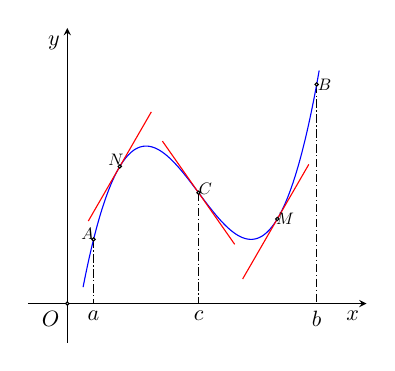
\begin{tikzpicture}
			\def\hsf(#1){((#1)^3-5*(#1)^2+7*(#1)-1}%ham so f
			\draw[-stealth,very thin](-.5,0)--(3.8,0)node[below left,scale=.8]{$x$};%truc Ox
			\draw[-stealth,very thin](0,-.5)--(0,3.5) node[below left,scale=.8]{$y$};%truc Oy
			\draw[fill=white](0,0)circle(.6pt)node[below left,scale=.8]{$O$};%goc toa do O
			\path (1/3,{\hsf(1/3)})coordinate(A) (19/6,{\hsf(19/6)})coordinate(B) (5/3,{\hsf(5/3)})coordinate(C)
			(8/3,{\hsf(8/3)})coordinate(M) (2/3,{\hsf(2/3)})coordinate(N);
			\draw[color=black,densely dash dot, thin] (A)--(1/3,0)node[below ,scale=.8] {$a$} (B)--(19/6,0)node[below ,scale=.8] {$b$} (C)--(5/3,0)node[below ,scale=.8] {$c$};
			\draw[blue,smooth,samples=100] plot[domain=.2:3.2](\x,{\hsf(\x)});
			\draw[red] (C)--+(125:.8)(C)--+(-55:.8) 
			(N)--+(60:.8)(N)--+(-120:.8) 
			(M)--+(60:.8)(M)--+(-120:.88);
			\foreach \p/\g in{A/140,B/0,C/30,M/0,N/120} \draw[fill=white](\p)circle(.6pt)+(\g:.1)node[scale=.6]{$\p$};
		\end{tikzpicture}
	\end{center}
	Điểm phân cách giữa cung lồi và cung lõm được gọi là \textbf{\color{diendantoanhoc}\itshape điểm uốn}. Điểm $C$ của đồ thị trong hình là điểm uốn.
	\vskip 0.1cm
	Nói cách khác thì: 
	Nếu hàm số $y=f(x)$ có đạo hàm trên khoảng $I$ ta nói rằng
	\vskip 0.1cm
	$a)$ Đồ thị ($C$) của hàm số $y = f(x)$ lồi trên khoảng $I$ nếu tiếp tuyến của ($C$) tại mỗi điểm của nó đều nằm phía trên đồ thị.
	\vskip 0.1cm
	$b)$ Đồ thị ($C$) của hàm số $ y = f(x)$ lõm trên khoảng $I$ nếu tiếp tuyến của nó tại mỗi điểm của nó đều nằm phía dưới đồ thị.
	\vskip 0.1cm
	\textbf{\color{diendantoanhoc}Nhận xét:} Một hàm được gọi là lồi (tương ứng, lõm) nếu đồ thị của nó là lồi (tương ứng, lõm). Đồ thị hàm lồi có hình dạng giống như một cái mũ $\cap $ còn của hàm lõm thì có hình dạng giống như một cái cốc  $\cup $.
	\vskip 0.1cm
	\textbf{\color{diendantoanhoc}$\pmb{2.}$ Dấu hiệu lồi, lõm và điểm uốn của đồ thị}
	\vskip 0.1cm
	Ta thừa nhận dấu hiệu lồi, lõm sau đây:
	\vskip 0.1cm
	\textbf{\color{diendantoanhoc}Định lý:} Cho hàm số $y = f(x)$ có đạo hàm đến cấp hai trên khoảng $I$.
	\vskip 0.1cm
	$1)$ Nếu $f "(x)< 0$ với mọi $x\in I$ thì đồ thị của hàm số \textbf{\color{diendantoanhoc}\itshape lồi} trên khoảng đó. 
	\vskip 0.1cm
	$2)$ Nếu $f "(x)> 0$ với mọi $x\in I$ thì đồ thị của hàm số  \textbf{\color{diendantoanhoc}\itshape lõm} trên khoảng đó.
	\vskip 0.1cm
	\textbf{\color{diendantoanhoc}Định lý:} Giả sử hàm số $y = f(x)$ có đạo hàm cấp hai trên một khoảng $I$ chứa điểm $ x _0$. Nếu $f"(x_0) = 0$ và $f"(x) $ đổi dấu khi $x$ qua điểm $x_0$ thì $U(x_0;f(x_0))$ là một điểm uốn của đồ thị hàm số $y = f(x)$.
	\vskip 0.1cm
	Tại điểm uốn tiếp tuyến đi xuyên qua đồ thị.
	\vskip 0.1cm
	\textbf{\color{diendantoanhoc}$\pmb{3.}$ Điều kiện để hai đường cong tiếp xúc nhau}
	\vskip 0.1cm
	Điều kiện để hai đường cong $y= f(x)$ và $y=g(x) $ tiếp xúc nhau là hệ phương trình sau có nghiệm và nghiệm của hệ là hoành độ giao điểm của hai đường cong đó \begin{align*}
		\begin{cases}f(x)=g(x)\\ f'(x)=g'(x)\end{cases}\tag{$*$}
	\end{align*}
	Vậy, đồ thị của $f$ và $g$ tiếp xúc nhau tại $x_0$ khi và chỉ khi $x_0$ là nghiệm của hệ ($*$).
	\vskip 0.1cm
	Thêm vào đó, nếu hai đường cong $y=f(x)$ và $y=g(x)$ có tính lồi lõm trái ngược nhau, ngoài ra có chung nhau tiếp tuyến thì khi đó phương trình $f(x)=g(x)$ có nghiệm duy nhất.
	\begin{center}
		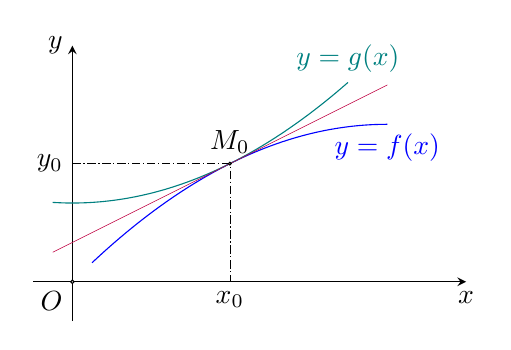
\begin{tikzpicture}
			\def\hsf(#1){-.125*(#1)^2+(#1)}%ham so f
			\def\hsg(#1){.125*(#1)^2+1}%ham so g
			\draw[-stealth] (-.5,0)--(5,0)node[below]{$x$};
			\draw[-stealth] (0,-.5)--(0,3)node[left]{$y$};
			\draw[fill=white](0,0)circle(.6pt)node[below left]{$O$};
			\draw[densely dash dot,very thin] (0,3/2)node[left]{$y_0$}-|(2,0) node[below]{$x_0$};
			\draw[smooth,blue]plot[domain=.25:4](\x,{\hsf(\x)}) node[below]{$y=f(x)$};
			\draw[smooth,teal]plot[domain=-.25:3.5](\x,{\hsg(\x)}) node[above]{$y=g(x)$};
			\draw[smooth,very thin,purple]plot[domain=-.25:4](\x,{.5*\x+1/2});
			\draw[fill=white](2,3/2)circle(.5pt)node[above]{$M_0$};
		\end{tikzpicture}
	\end{center}
	Cần phải chú ý rằng nhiều tài liệu trong và ngoài nước hiện nay định nghĩa về tính lồi (convex), lõm (concave) của đồ thị hàm số khác như đã nêu ở trên. Cụ thể là hàm lồi trong bài viết này được gọi là hàm lõm trong một số tài liệu, còn hàm lõm trong bài viết này thì lại được họ gọi là hàm lồi. 
	\vskip 0.1cm
	\textit{\textbf{\color{diendantoanhoc}Ta sẽ vận dụng những tính chất và nhận xét trên để ứng dụng trong việc giải một số bài toán về phương trình, bất phương trình, đây cũng chính là cở sở của phương pháp tiếp tuyến trên}}.
	\vskip 0.1cm
	Trong bài viết này chúng ta viết tắt VT cho vế trái, VP cho vế phải.
	Việc kiểm tra dấu hiệu lồi, lõm của hàm số bằng cách tính đạo hàm cấp hai trong một số ví dụ sẽ được dành cho bạn đọc.
	\vskip 0.1cm
	\textbf{\color{diendantoanhoc}$\pmb{4.}$ Các ví dụ}
	\vskip 0.1cm
	\textbf{\color{diendantoanhoc}Ví dụ $\pmb{1.}$} Giải phương trình
	\begin{align*}
		x^2-2x+5=\sqrt{x+3}+\sqrt{5-x}.
	\end{align*}
	\textit{Lời giải.} Điều kiện $-3\leq x\leq 5$. Vế trái là hàm lõm còn vế phải là hàm lồi (bạn đọc tự kiểm tra), chúng có chung tiếp tuyến tại $(1;4)$. Vậy $x=1$ là nghiệm duy nhất của phương trình.
	\vskip 0.1cm
	\textbf{\color{diendantoanhoc}Nhận xét:} Bài tập kiểu như trên rất quen thuộc với nhiều bạn đọc, phương pháp thường dùng là đánh giá bất đẳng thức. Ở đây, chúng ta sử dụng tiếp cận khác thông qua tiếp tuyến.
	\vskip 0.1cm
	Ta sẽ đến với những ví dụ khác, đòi hỏi đến cả kỹ năng nhẩm nghiệm.
	\vskip 0.1cm
	\textbf{\color{diendantoanhoc}Ví dụ $\pmb{2.}$} Giải phương trình
	\begin{align*}
		\sqrt[6]{6x-5}=\dfrac{x^{7}}{8x^{2}-10x+3}.
	\end{align*}
	\textit{Lời giải.} Điều kiện $x\ge \frac{5}{6}$. Với $x\ge \frac{5}{6}$ thì $VT$ là hàm lồi, liên tục, vì vậy đồ thị hàm số nằm dưới tiếp tuyến của nó tại điểm $x=1$ là $y=x+1$.
	Với $x\ge\frac{5}{6}$ thì $VP$ là hàm lõm, liên tục, vì vậy đồ thị hàm số nằm trên tiếp tuyến của nó tại điểm $x=1$ là $y=x+1$.
	\vskip 0.1cm
	Vậy $x=1$ là nghiệm duy nhất của phương trình. 
	\vskip 0.1cm
	\textbf{\color{diendantoanhoc}Ví dụ $\pmb{3.}$} Cho hai hàm số $f(x)$ và $g(x)$ được xác định như sau: $f(x)=\sqrt{13x^{2} - 6x + 10 } + \sqrt{5x^{2} -13x + \frac{17}{2}} + \sqrt{17x^{2} - 48x + 36} $ và $g(x)= \dfrac{1}{2}(36x - 8x^{2} - 21)$.
	\vskip 0.1cm
	Giải phương trình $f(x)=g(x)$.
	\vskip 0.1cm
	\textit{Lời giải.} Điều kiện $x\in \mathbb R$. Đặt $h(x)=f(x)-g(x)$\\ Không khó để chỉ ra $h(x)$ là hàm lõm, liên tục. Nhận thấy $h(\dfrac{3}{2})=0$ và $h'(\dfrac 32)=0$ , do đó đồ thị hàm số tiếp xúc với trục hoành tại điểm $x=\dfrac{3}{2}$.
	\vskip 0.1cm
	Vậy $x=\dfrac{3}{2}$ là nghiệm duy nhất của phương trình của bài toán.
	\vskip 0.1cm
	\textbf{\color{diendantoanhoc}Ví dụ $\pmb{4.}$} Giải phương trình
	\begin{align*}
		x\sqrt{x^2\!+\!6}\!+\!(x\!+\!1)\sqrt{x^2\!+\!2x\!+\!7}\!=\!\dfrac{13}{5}(2x\!+\!1)
	\end{align*}
	\textit{Lời giải.}  Điều kiện $x\in\mathbb R$. Đặt $g(x)=x\sqrt{x^2+6}$ và $f(x)=g(x+1)+g(x)$.
	\vskip 0.1cm
	Ta dễ kiểm tra thấy rằng:
	\vskip 0.1cm
	$a)$ $g(x)$ là hàm lẻ và $g''(x)$ cũng là hàm lẻ; hơn nữa ta cũng có $f(-\dfrac 12)=f''(-\dfrac 12)=0$.
	\vskip 0.1cm
	$b)$ $g(x)$ và $g''(x)$ là hàm đồng biến, suy ra $f(x)$ và $f''(x)$ cũng là hàm đồng biến.
	\vskip 0.1cm
	$c)$ Tiếp tuyến với đồ thị của hàm số  $f(x)$ tại $x=-\dfrac 12$ là $y=\dfrac{13}5(2x+1)$.
	\vskip 0.1cm
	Vậy đồ thị hàm số $f(x)$ nằm dưới tiếp tuyến của nó khi $x<-\dfrac 12$ và đồ thị hàm số $f(x)$ nằm trên tiếp tuyến của nó khi $x>-\dfrac 12$.
	\vskip 0.1cm
	Vậy $x=-\dfrac{1}{2}$ là nghiệm duy nhất của phương trình.
	\vskip 0.1cm
	\textbf{\color{diendantoanhoc}Chú ý:} Ở ví dụ này nghiệm của phương trình chính là hoành độ điểm uốn của đồ thị.
	\vskip 0.1cm
	\textbf{\color{diendantoanhoc}Ví dụ $\pmb{5.}$} Giải phương trình
	\begin{align*}
		&3\left(x^{3}+\frac{x}{\sqrt{\left(1+x^{2} \right)^{3}}} \right)+2\\
		=\,\,&\sqrt{\left(1+x \right)^{3}}+\sqrt{\left(1-x \right)^{3}}.
	\end{align*}
	\textit{Lời giải.}  Điều kiện xác định $x\in[-1;1]$. Nhận xét rằng $x=0$ là một nghiệm của phương trình. Đặt $f(x)=x+(1+x)^{-\frac 32}$ và $g(x)=\dfrac{(1+x)^{\frac 32}+(1-x)^{\frac 32}-2}x$.
	\vskip 0.1cm
	Giả sử $x\ne 0$. Phương trình đã cho có thể được viết lại thành $3f(x^2)=g(x)$.
	\vskip 0.1cm
	Chú ý rằng:
	\vskip 0.1cm
	Một mặt, $g(x)$ là hàm lẻ, nhận giá trị âm trên $[-1;0)$ và dương trên $(0, 1]$ và đồng biến trên mỗi khoảng này (bạn đọc tự kiểm tra), nên $g(x)\le g(1)=2\sqrt 2-1 <1$ với mọi $0\ne  x\in[-1,1]$.
	\vskip 0.1cm
	Mặt khác, $f(x)$ là hàm lõm trên $[0,1]$ (bạn đọc tự kiểm tra), vì vậy đồ thị hàm số nằm trên tiếp tuyến của nó tại điểm $x=0$ : $f(x)\ge 1-\frac x2\ge \frac 12$.
	\vskip 0.1cm
	Vậy $f(x^2)\ge \frac 12$, suy ra $3f(x^2)\ge \frac 32 > 1\ge g(x)$, do đó phương trình không còn nghiệm nào nữa. 
	\vskip 0.1cm
	Vậy $x=0$ là nghiệm duy nhất của phương trình đã cho.
	\vskip 0.1cm
	\textbf{\color{diendantoanhoc}Ví dụ $\pmb{6.}$} Cho số lẻ $n>1$. Giải phương trình
	\begin{align*}
		n^{x^n-1}+n^{\frac{1}{x}}=n+1.
	\end{align*}
	\textit{Lời giải.} Điều kiện xác định: $x \neq 0$. 
	Nếu $x<0$ thì VT$<2<$VP nên trường hợp này phương trình vô nghiệm.
	\vskip 0.1cm
	Xét trường hợp $x>0$. Xét hàm số $f(x):\mathbb R^+\to \mathbb R$ xác định bởi:
	\begin{align*}
		f(x)=n^{x^n-1}+n^{\frac 1x}-n-1
	\end{align*}
	Ta lần lượt có:
	\begin{align*}
		f'(x)=&\,n(\ln n)x^{n-1}n^{x^n-1}-\frac {\ln n}{x^2}n^{\frac 1x}.\\
		f''(x)=&\,n(\ln n)\left(n(\ln n)x^{2n-2}+(n-1)x^{n-2}\right)\\
		&\times n^{x^n-1}+\ln n\left(\frac {\ln n}{x^4}+\frac 2{x^3}\right)n^{\frac 1x}.
	\end{align*}
	Nhận thấy rằng $f(1)=f'(1)=0$, do đó tiếp tuyến của hàm số $f(x)$ tại điểm $x=1$ là trục hoành.
	\vskip 0.1cm 
	Vì $f(x)$ là hàm lõm và liên tục ($f''(x)>0$) do đó $x=1$ là nghiệm duy nhất của phương trình. 
	\vskip 0.1cm
	\textbf{\color{diendantoanhoc}Ví dụ $\pmb{7.}$} Giải bất phương trình
	\begin{align*}
		45x^3\!-\!17x^2\!-\!37x\!+\!25\!\ge\! 4\sqrt{\!\!(x\!+\!1)(5x\!-\!3)^3}.
	\end{align*}
	\textit{Lời giải.} Bất phương trình đã cho được viết lại thành 
	\begin{align*}
		(x\!+\!1\!)(45x^2\!-\!62x\!+\!25)\!\ge\! 4\sqrt{\!\!(x\!+\!1\!)(5x\!-\!3)^3}.
	\end{align*}
	Nhận thấy rằng một nghiệm là $x=-1$; các nghiệm khác phải thỏa mãn $x>-1$ (trái lại thì VT$<0\le$ VP), và thật ra $x\ge\frac 35$ (trái lại thì VP không xác định).
	\vskip 0.1cm
	Khi đó (với điều kiện $x\ge\frac 35$) bất phương trình trở thành
	\begin{align*}
		45x^2-62x+25\ge 4(5x-3)\sqrt{\dfrac{5x-3}{x+1}}.
	\end{align*}
	Nhận thấy một nghiệm thứ hai là $x=\frac 35$. Vậy với $x>\frac 35$ bất phương trình trở thành
	\begin{align*}
		\dfrac{45x^2-62x+25}{4(5x-3)}\ge \sqrt{\dfrac{5x-3}{x+1}}.
	\end{align*}
	VT là hàm lõm (bạn đọc tự kiểm tra) với tiếp tuyến $y=x$ tại $x=1$, VP là hàm lồi (bạn đọc tự kiểm tra) với tiếp tuyến $y=x$ tại $x=1$. Vậy đồ thị hàm số VT luôn nằm trên đồ thị của VP,  do đó bất phương trình luôn đúng.
	\vskip 0.1cm
	Vậy nghiệm của bất phương trình là: \linebreak $x\in\{-1\}\cup\left[\frac 35,+\infty\right)$
	\vskip 0.1cm
	\textbf{\color{diendantoanhoc}$\pmb{5.}$ Bài tập đề nghị}
	\vskip 0.1cm
	\textbf{\color{diendantoanhoc}Bài $\pmb{1.}$} Giải các phương trình sau trên tập số thực
	\vskip 0.1cm
	$a)$  $\sqrt[4]{x}=\frac{3}{8}+2x$.
	\vskip 0.1cm
	$b)$ $8x^2+\sqrt{\frac{1}{x}}=\frac{5}{2}.$
	\vskip 0.1cm
	$c)$ $16x^4+5=6\sqrt[3]{4x^3+x}.$
	\vskip 0.1cm
	$d)$ $ 2\sqrt[4]{\dfrac{x^{2}}{3}+4}=1+\sqrt{\dfrac{3x}{2}}.$
	\vskip 0.1cm
	$e)$ $x^2+2x+4=3\sqrt{x^3+4x}.$
	\vskip 0.1cm
	$f)$ $2^{x^2}+3^{x^2}+4^{x^2}+5^{x^2}=4^{1-x^2}.$
	\vskip 0.1cm
	$g)$ $x^2+x = (6x-x^2-2)\sqrt{x-1}.$
	\vskip 0.1cm
	$h)$ $2x^2-11x+21-3\sqrt[3]{4x-4}=0.$
	\vskip 0.1cm
	$i)$ $x^{3}+x^{2}-15x+30=4\sqrt[4]{27(x+1)}.$
	\vskip 0.1cm
	$j)$ $2\sqrt[4]{27x^2+24x+\frac{28}{3}}=1+\sqrt{\frac{27x}{2}+6}.$
	\vskip 0.1cm
	$k)$ $\sqrt{x^2+x-1}+\sqrt{x-x^2+1}=x^2-x+2.$
	\vskip 0.1cm
	$l)$ $x^2-2x+3=\sqrt{2x^2-x}+\sqrt{1+3x-3x^2}.$
	\vskip 0.1cm
	$m)$ $\sqrt{x^2+x+19}+\sqrt{7x^2+22x+28}$\\
	$\quad\,\,+\sqrt{13x^2+43x+37}=3\sqrt{3}(x+3)$.
	\vskip 0.1cm
	$n)$ $\log_2 \dfrac{2x+1}{4x} = \log_{x} \dfrac{2x+1}{2}.$\\
	\vskip 0.1cm
	\textbf{\color{diendantoanhoc}Bài $\pmb{2.}$} Tồn tại hay không các cặp số thực âm $(x,y)$ thoả mãn phương trình \linebreak$x2^y+y2^{-x}=x+y$?
	\vskip 0.1cm
	\textbf{\color{diendantoanhoc}Bài $\pmb{3.}$} Tìm tất cả các số thực $a$ sao cho bất phương trình $a^x\geq 1+x\log _{11}12$ đúng với mọi số thực $x$.
	\vskip 0.1cm
	\textbf{\color{diendantoanhoc}Tài liệu tham khảo}
	\vskip 0.1cm
	[$1$] Ngô Thúc Lanh (chủ biên), {\it Giải tích $12$ }(SGK), Nhà xuất bản Giáo Dục ($2006$).
	\vskip 0.1cm
	[$2$] Nguyễn Huy Đoan (chủ biên), {\it Giải tích $12$ nâng cao} (SGK), Nhà xuất bản Giáo Dục ($2008$).
	\vskip 0.1cm
	[$3$] Phan Đức Chính (chủ biên), {\it Một số phương pháp chọn lọc giải các bài toán sơ cấp (Tập $2$)}, Nhà xuất bản Đại học Quốc gia Hà Nội ($2003$). 
	\vskip 0.1cm
	[$4$] Nguyễn Quang Nam, {\it Kỹ thuật tạo nhân tử kép}, Tạp chí Toán học và Tuổi trẻ, Nhà xuất bản Giáo Dục (Số $511$, tháng $1/2020)$.
	\vskip 0.1cm
	[$5$]~\url{https://artofproblemsolving.com/com} \url{munity}
	\end{multicols}
%\newpage

%
%	\setcounter{figure}{0}
%	\thispagestyle{doisongtoanhocnone}
\pagestyle{doisongtoanhoc}
\everymath{\color{doisongtoanhoc}}
\graphicspath{{../doisongtoanhoc/pic/}}
%\blfootnote{$^1$\color{doisongtoanhoc}Trung tâm Thông tin -- Tư liệu, Viện Hàn lâm Khoa học và Công nghệ Việt Nam.}
\begingroup
\AddToShipoutPicture*{\put(0,616){\includegraphics[width=19.3cm]{../bannerdoisong}}}
\AddToShipoutPicture*{\put(43,527){\includegraphics[scale=0.95]{../tieude.pdf}}}\centering
\endgroup

\vspace*{185pt}


\begin{multicols}{2}	
	Đại hội Toán học Quốc tế (International Congress of Mathematicians, sau đây sẽ viết tắt là ICM) là sự kiện khoa học quan trọng hàng đầu của các nhà toán học trên thế giới. Nhiều người trong chúng ta đã quen thuộc với Kỳ thi Olympic Toán quốc tế (IMO). Vậy ICM có gì giống và khác với IMO? Mục đích của ICM là gì? Những hoạt động chính tại một kỳ ICM là gì? ICM $2022$ có những dấu ấn gì đặc biệt? Chúng tôi sẽ thử giải đáp các câu hỏi này.
	\vskip 0.1cm
	$\pmb{1.}$ \textbf{\color{doisongtoanhoc}ICM có gì giống và khác với IMO?}
	\vskip 0.1cm
	Cũng giống như IMO, ICM là một hoạt động cộng đồng hướng đến mục tiêu phát triển sự quan tâm đến toán học. Có lịch sử lâu đời hơn IMO một chút, ICM đầu tiên được tổ chức từ năm $1897$ tại Z\"urich, Thụy Sĩ, nhưng trong khi IMO được tổ chức hầu như hằng năm, thì ICM được tổ chức bốn năm một lần. Nếu IMO tập trung vào việc giải các bài toán, thì ICM hướng đến trình bày những thành tựu nghiên cứu toán học đáng kể nhất gần đây. Không có sự khác biệt đáng kể giữa nghiên cứu toán học và giải các bài toán Olympic, vì cả hai công việc đều đòi hỏi kỹ năng giải quyết vấn đề. Chúng ta biết rằng có những bài toán mở nổi tiếng trong toán học, như  định lý lớn Fermat (là bài toán mở đến trước $1994$), giả thuyết về số nguyên tố sinh đôi, hay giả thuyết Riemann (cả hai hiện vẫn chưa được giải quyết). Những tiến bộ về các bài toán mở nổi tiếng, nếu có, cũng là một điểm nhấn quan trọng của những kỳ ICM. Nhưng so với việc thi olympic, có thể nói các nhà toán học có nhiều tự do hơn trong việc làm nghiên cứu của mình, họ không nhất thiết phải làm việc với một vấn đề có sẵn. Có những nhà toán học lớn theo đuổi một vấn đề  hàng năm, thậm chí hàng chục năm trời. Việc một nhà số học ngồi nghe một bài giảng hình học đại số, hay một nhà đại số dự một bài giảng vật lý toán, để mở mang kiến thức, cũng là một việc thường xảy ra và được ICM khuyến khích.
	\vskip 0.1cm
	$\pmb{2.}$ \textbf{\color{doisongtoanhoc}Vì sao cần tổ chức ICM?}
	\vskip 0.1cm
	Mục đích chính của ICM là để tạo điều kiện cho các nhà toán học từ khắp nơi trên thế giới gặp gỡ những chuyên gia hàng đầu, và để tôn vinh những thành tựu toán học nổi bật nhất gần đây.
	\vskip 0.1cm
	Các nhà toán học gặp gỡ nhau? Chẳng phải các nhà toán học chỉ cần có giấy bút (và máy tính) để làm việc đó sao? Đúng là phần lớn các nhà toán học  có thiên hướng lý thuyết,  không cần nhiều trang thiết bị để làm việc. Nhưng ngoài giấy bút và máy tính, họ cũng thường cần một người đồng nghiệp ăn ý để thử nghiệm những ý tưởng chợt đến, tranh cãi về một chứng minh trong một bài báo, hay đơn giản tán gẫu về trận bóng tối qua. 
	\vskip 0.1cm
	Như bất cứ ngành khoa học có truyền thống nào, toán học ngày càng đa dạng hóa và chuyên môn hóa cao độ, với rất nhiều phân ngành khác nhau. ICM đầu tiên năm $1897$ chỉ có năm tiểu ban, mỗi tiểu ban phụ trách một chuyên môn, gồm có số học và đại số, giải tích và lý thuyết hàm, hình học, cơ học và vật lý toán, lịch sử và thư mục toán học. Nửa thế kỷ sau, ICM $1958$ mới có tám tiểu ban\footnote{\color{doisongtoanhoc}Xem Guillermo P. Curbera, \emph{Mathematicians of the World, Unite!}, Wellesley, Massachusetts: A.K. Peters, Ltd ($2009$), trang $14$ và $141$.}. Đến ICM $2022$, ta có đến hai mươi tiểu ban: logic, đại số, hình học đại số và hình học phức, tôpô, lý thuyết Lie và các mở rộng, giải tích, động lực học, phương trình vi phân, vật lý toán... Mỗi tiểu ban ngày nay lại có nhiều tiểu mục nhỏ hơn, ví dụ tiểu ban đại số có bốn tiểu mục.  Ngay từ ICM năm $1908$ ở Rome, Poincar\'e đã nhận ra: ``Khi một khoa học càng phát triển, ta càng khó nắm bắt được toàn bộ khoa học đó. Từ đó người ta phải chia nhỏ khoa học ấy ra nhiều phần, và bằng lòng với việc chỉ quan tâm tới đúng một trong các phần đó, nói cách khác là phải chuyên môn hóa. Chuyên môn hóa quá sâu sẽ làm cản trở nghiêm trọng đến tiến bộ chung của khoa học (...) Chính nhờ những tương tác bất ngờ giữa các hướng nghiên cứu khác nhau mà khoa học mới có thể phát triển."\footnote{\color{doisongtoanhoc}``In proportion as the science develops, it becomes more difficult to take it in its entirety. Then an attempt is made to
		cut it in pieces and to be satisfied with one of these pieces -- in
		a word, to specialize. Too great a movement in this direction
		would constitute a serious obstacle to the progress of science. As I have said, it is by unexpected concurrences
		between its different parts that it can make progress." Xem The Mathematical Intelligencer, Tập $34$, số $2$ ($2012$), trang $15-29$.} Nhà toán học nổi tiếng Hoàng Tụy ($1927-2019$) sinh thời thường cảnh báo về nguy cơ của chủ nghĩa tỉnh lẻ, khi một nhà khoa học làm việc trong tinh thần bế quan tỏa cảng và khiến bản thân thui chột. Gặp gỡ và tương tác với những chuyên gia hàng đầu tại những sự kiện lớn như ICM là cách giúp một nhà khoa học ``mở con mắt hướng ra những bờ cõi khoa học nơi những người khác đang chiếm cứ, và buộc ta phải so sánh thành tựu của mình với họ, qua đó nhận ra ngôi làng mình đang sống nhỏ bé chừng nào", theo lời của Poincar\'e\footnote{\color{doisongtoanhoc}Tài liệu đã dẫn, trang $20$.}.
	\vskip 0.1cm
	$\pmb{3.}$ \textbf{\color{doisongtoanhoc}Hoạt động chính ở các ICM là gì?}
	\vskip 0.1cm
	Hoạt động chính của ICM là các bài giảng của các chuyên gia, và phần trao giải thưởng ghi nhận những thành tựu toán học cao nhất đã đạt được giữa hai kỳ đại hội. Các bài giảng của chuyên gia gồm hai loại là các bài giảng toàn thể (khoảng $20$ bài) và các bài giảng tiểu ban (khoảng 180 bài). Được đọc bài giảng tại một ICM là một vinh dự lớn, nếu ta biết rằng mỗi năm có khoảng gần một trăm nghìn công trình toán học được xuất bản trên các tạp chí chuyên ngành. Các giải thưởng được trao ở các kỳ ICM gần đây là huy chương Fields (cho nhà toán học trẻ xuất sắc), giải thưởng Nevanlinna (khía cạnh toán học trong tin học), giải Gauss (toán ứng dụng), huy chương Chern (những người có thành tựu toán học xuất chúng, không hạn chế tuổi tác), và giải Leelavati (phổ biến kiến thức và quảng bá toán học). Trong số này, huy chương Fields nói chung được coi là giải thưởng danh giá nhất.
	\vskip 0.1cm
	$\pmb{4.}$ \textbf{\color{doisongtoanhoc}Ai có thể giành được huy chương Fields?}
	\vskip 0.1cm
	Huy chương Fields được trao cho những nhà toán học dưới $40$ tuổi với thành tựụ xuất sắc và tiềm năng phát triển lớn. Nhìn vào những người đoạt huy chương Fields gần đây, ta thấy họ nói chung là những người tài năng, được đào tạo bài bản (có bằng tiến sĩ), và theo đuổi những lĩnh vực quan trọng hoặc những bài toán quan trọng trong một thời gian dài. Có lẽ cách chắc chắn nhất để \emph{không} giành được giải Fields là lao vào những bài toán nổi tiếng, nhiều người biết, như giả thuyết Collatz, hay giả thuyết Riemann, bằng tay không, không quan tâm đến việc tích lũy kiến thức và các kỹ thuật cơ bản dần dần. Những huy chương Fields, ngoài sự dũng cảm tấn công những vấn đề khó khăn, còn ghi dấu ấn cụ thể, thuyết phục với những bài báo với nhiều người đọc, được bình duyệt chặt chẽ, trên những tạp chí toán học uy tín. Thông thường họ đã có một công chúng rộng lớn, những ý tưởng của họ đã có ích lợi đáng kể cho công việc của nhiều người khác, \emph{trước khi} được vinh danh với huy chương Fields, chứ không phải ngược lại. Tất nhiên không có quy tắc chung cho những tài năng đặc biệt, họ thường  phá vỡ những quy tắc mà chúng ta coi như hiển nhiên.
	\vskip 0.1cm
	$\pmb{5.}$ \textbf{\color{doisongtoanhoc}Đại hội Toán học Quốc tế $2022$ có gì đặc biệt?}
	\vskip 0.1cm
	ICM $2022$ được tổ chức từ ngày mùng $6$ đến $14/7/2022$. Lễ trao các giải thưởng được tổ chức trực tiếp tại Helsinki, Phần Lan vào ngày $5/7$. Về hình thức, sau $125$ năm lịch sử, đây là lần đầu tiên chương trình khoa học của ICM được tổ chức theo hình thức trực tuyến. Tại ICM năm nay, huy chương Fields đã được trao cho Hugo Dominil--Copin (Pháp), June Huh (Hàn Quốc), James Maynard (Vương quốc Anh), và Maryna Viazovska (Ukraina). Đây đều là những tên tuổi hàng đầu của toán học đương đại, những người sẽ còn tiếp tục ảnh hưởng lâu dài đến toán học. Nếu bạn nghĩ một bài giảng toán học là đối cực của một tiểu thuyết hấp dẫn/một bộ phim hay? Mời bạn xem bài giảng hết sức sáng sủa với đoạn cao trào tuyệt vời của June Huh, một người làm toán (những bài toán không hề đơn giản!) với hồn thơ đặc biệt. Nếu bạn, sau khi sở hữu một cỗ máy tiêu diệt hàng loạt các loại bài toán khó muôn hình vạn trạng, nghĩ quảng bá toán học là một việc nhàm chán và không cần công phu gì? Mời bạn xem bài giảng của Nikolai Andreev (giải Leelavati $2022$) và trang mạng độc đáo của ông\footnote{\color{doisongtoanhoc}https://etudes.ru/}.
	\vskip 0.1cm
	Trong một thế giới còn rất nhiều xung đột và đối kháng, các kỳ ICM và Liên đoàn Toán học Quốc tế (IMU) hướng đến gắn kết con người bằng toán học và tinh thần quốc tế, vượt qua những giới hạn về tư tưởng, ngôn ngữ, văn hóa, mặc cảm thượng đẳng/mặc cảm thấp kém thường ám ảnh con người. Từ khi kỳ ICM đầu tiên được tổ chức đến nay, toán học đã gánh chung tác động của hai thế chiến, chiến tranh lạnh, kỳ thị và phân biệt đối xử, với những hoạt động khác của con người. Vượt qua những khó khăn đó, cộng đồng toán học đã tiếp tục đi tới với lý tưởng bình đẳng, nhân văn, và chủ nghĩa quốc tế, di sản to lớn của những nhà toán học hàng đầu trong quá khứ. Chúng ta hy vọng vào thành công trong tương lai của toán học và của những lý tưởng này.
\end{multicols}

%	\newpage

%	\setcounter{figure}{0}
%	\thispagestyle{toanhocvadoisongnone}
\pagestyle{toanhocvadoisong}
\everymath{\color{toanhocdoisong}}
\graphicspath{{../toanhocdoisong/pic/}}
\begingroup
\blfootnote{$^1$\color{toanhocdoisong}Viện Sinh thái và Môi trường Đông Dương.}
\AddToShipoutPicture*{\put(0,616){\includegraphics[width=19.3cm]{../bannertoanhocdoisong}}}
\AddToShipoutPicture*{\put(79,520){\includegraphics[scale=1]{../tieude.pdf}}}
\centering
\endgroup

\vspace*{190pt}

\begin{multicols}{2}
	Bài toán cây kim của Buffon vẫn luôn xuất hiện trong sách giáo khoa toán dưới dạng một phương pháp để tính số $\pi$. Trong bài này, chúng ta hãy cũng Pi tìm hiểu chi tiết về bài toán này cũng như một số ứng dụng thú vị của nó trong thực tiễn.
	
	\vskip 0.1cm
	\textbf{\color{toanhocdoisong}$\pmb{1.}$ Bài toán cây kim của Buffon}
	\begin{figure}[H]
		\vspace*{-5pt}
		\centering
		\captionsetup{labelformat= empty, justification=centering}
		\includegraphics[width=0.6\linewidth]{1}
		\caption{\small\textit{\color{toanhocdoisong}Georges--Louis Leclerc, Comte de Buffon $(1707-1788)$.}}
		\vspace*{-10pt}
	\end{figure}
	Nhà toán học Pháp thế kỉ $18$, Georges Louis Leclerc, được phong Bá tước tại vùng có một ngôi làng tên Buffon nên ông còn có danh hiệu Comte de Buffon (Bá tước Buffon). Do đó các tài liệu thường gọi tắt là Buffon. Bài toán nổi tiếng mang tên ông có nội dung như sau:
	\vskip 0.1cm
	``Trên một tờ giấy với các đường kẻ cách đều nhau khoảng cách $d$, thả ngẫu nhiên một cây kim chiều dài $l$ $(d>l)$, hãy tìm xác suất để cây kim cắt một đường nằm ngang trên trang giấy".
	\begin{figure}[H]
		\vspace*{-5pt}
		\centering
		\captionsetup{labelformat= empty, justification=centering}
		\includegraphics[width=0.95\linewidth]{2}
		\caption{\small\textit{\color{toanhocdoisong}Hình $1$. Minh họa bài toán cây kim của Buffon.}}
		\vspace*{-10pt}
	\end{figure}
	Chúng ta hãy xét một lời giải không sử dụng tích phân được E. Barbier đưa ra năm $1860$.
	\vskip 0.1cm 
	Do $l<d$ nên chỉ có hai trường hợp xảy ra: cây kim cắt một đường kẻ và cây kim không đè lên đường kẻ nào; không tồn tại trường hợp cây kim cắt nhiều hơn một đường kẻ.
	\vskip 0.1cm
	Gọi $P(l)$ là xác suất để cây kim có độ dài $l$ cắt một đường kẻ khi được thả. Lấy một điểm bất kỳ trên cây kim chia nó thành hai đoạn thẳng độ dài $l_1$ và $l_2$. Ta có:
	\begin{align*}
		P(l)=P(l_1 )+P(l_2).
	\end{align*}
	Quan hệ trên có thể được mở rộng ra thành dạng $P(l)=n\cdot P(\dfrac{l}{n})$. Tức là xác suất để một cây kim cắt đường kẻ khi được thả sẽ bằng $n$ lần xác suất này của cây kim có độ dài bằng $\dfrac{1}{n}$ lần độ dài cây kim ban đầu.
	\vskip 0.1cm
	Do đó, $P(l)=c\cdot l$ với $c$ là một hằng số, $c=P(1)$ (khi $l=1$ và $d > 1$).
	\begin{figure}[H]
		\vspace*{-5pt}
		\centering
		\captionsetup{labelformat= empty, justification=centering}
		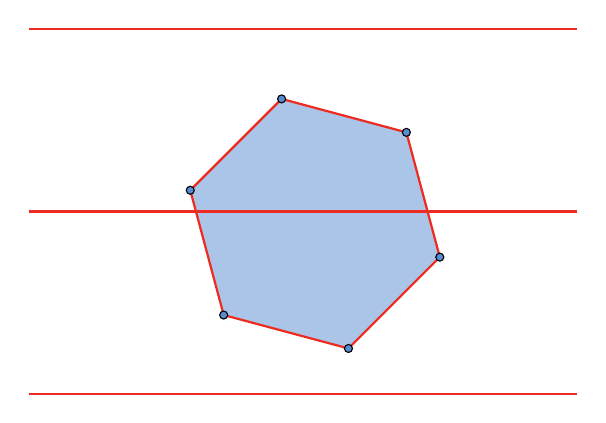
\begin{tikzpicture}[scale=0.58]
			\definecolor{qqqqff}{rgb}{0.,0.,1.}
			\definecolor{ududff}{rgb}{0.30196078431372547,0.30196078431372547,1.}
				\fill[line width=0.8pt,color=cackithi,fill=cackithi,fill opacity=0.5] (1.,3.) -- (3.,5.) -- (2.267949192431123,7.732050807568878) -- (-0.46410161513775494,8.464101615137755) -- (-2.4641016151377553,6.464101615137756) -- (-1.7320508075688794,3.7320508075688785) -- cycle;
				\draw [line width=0.8pt,color=toanhocdoisong] (1.,3.)-- (3.,5.);
				\draw [line width=0.8pt,color=toanhocdoisong] (3.,5.)-- (2.267949192431123,7.732050807568878);
				\draw [line width=0.8pt,color=toanhocdoisong] (2.267949192431123,7.732050807568878)-- (-0.46410161513775494,8.464101615137755);
				\draw [line width=0.8pt,color=toanhocdoisong] (-0.46410161513775494,8.464101615137755)-- (-2.4641016151377553,6.464101615137756);
				\draw [line width=0.8pt,color=toanhocdoisong] (-2.4641016151377553,6.464101615137756)-- (-1.7320508075688794,3.7320508075688785);
				\draw [line width=0.8pt,color=toanhocdoisong] (-1.7320508075688794,3.7320508075688785)-- (1.,3.);
				\draw [toanhocdoisong,line width=0.8pt] (-6.,6.)-- (6.,6.);
				\draw [toanhocdoisong,line width=0.8pt] (-6.,2.)-- (6.,2.);
				\draw [toanhocdoisong,line width=0.8pt] (-6.,10.)-- (6.,10.);
			
				\draw [fill=cackithi] (1.,3.) circle (2.5pt);
				\draw [fill=cackithi] (3.,5.) circle (2.5pt);
				\draw [fill=cackithi] (2.267949192431123,7.732050807568878) circle (2.5pt);
				\draw [fill=cackithi] (-0.46410161513775494,8.464101615137755) circle (2.5pt);
				\draw [fill=cackithi] (-2.4641016151377553,6.464101615137756) circle (2.5pt);
				\draw [fill=cackithi] (-1.7320508075688794,3.7320508075688785) circle (2.5pt);
		\end{tikzpicture}
		\caption{\small\textit{\color{toanhocdoisong}Hình $2$. Thả một đa giác cạnh $l$ lên tờ giấy với các đường kẻ ngang cách đều nhau.}}
		\vspace*{-10pt}
	\end{figure}
	Ta hãy tiếp tục xét một đa giác đều $N$ cạnh có độ dài mỗi cạnh bằng $l$ (Hình $2$). Ta đã biết ở trên rằng xác suất để mỗi cạnh của đa giác cắt một đường kẻ là $P(l)$. Đây cũng chính là giá trị kỳ vọng của số giao điểm của một cạnh với các đường kẻ, vì số giao điểm nói chung chỉ có thể là $0$ hoặc $1$ tương ứng với không cắt và cắt. Theo tính chất cộng tính của kỳ vọng, giá trị kỳ vọng của số giao điểm của đa giác với các đường kẻ khi thả lên tờ giấy là:
	\begin{align*}
		E &= \sum\nolimits_{i = 1}^N {P(l) = N \cdot } P(l) \\
		&= N \cdot c \cdot l = c \cdot L, \tag{$1$}
	\end{align*}
	với $L=N \cdot l$ là chu vi của đa giác đều.
	\vskip 0.1cm
	\columnbreak
	\PIbox{\textbf{\color{toanhocdoisong}Giá trị kỳ vọng}
		\vskip 0.1cm
		Trong một thí nghiệm ngẫu nhiên, nếu kết quả có giá trị $x_i$ có xác suất xảy ra là $p_i$ thì giá trị kỳ vọng của kết quả thu được được tính theo công thức:
		\setlength{\abovedisplayskip}{4pt}
		\setlength{\belowdisplayskip}{4pt}
		\begin{align*}
			E=x_1 p_1+x_2 p_2+ \cdots +x_n p_n.
		\end{align*}
		Ví dụ, với thí nghiệm gieo con xúc xắc, giá trị kỳ vọng của số chấm thu được là:
		\begin{align*}
			E=\frac{1}{6}\cdot 1 + \frac{1}{6} \cdot 2 + \cdots + \frac{1}{6}\cdot6 = 3{,5}.
		\end{align*}
		Chú ý rằng giá trị kỳ vọng có thể không trùng với một trong các giá trị có thể xảy ra. Theo định luật số lớn trong xác suất, với số lần thực hiện thí nghiệm càng lớn thì giá trị trung bình của các kết quả sẽ càng đến gần với giá trị kỳ vọng.}
	\vskip 0.1cm
	Mặt khác, nếu giữ chu vi $L$ của đa giác không đổi, khi $N \to \infty$, đa giác của ta sẽ trở thành một đường tròn có chu vi $L$ và bán kính $\dfrac{L}{2\pi}$.
	\vskip 0.1cm
	Để tính hệ số $c$, ta xét một trường hợp đặc biệt, khi đường tròn có đường kính đúng bằng khoảng cách $d$ giữa các dòng kẻ. Khi đó, ta có $L=\pi d$.
	\begin{figure}[H]
		\vspace*{-5pt}
		\centering
		\captionsetup{labelformat= empty, justification=centering}
		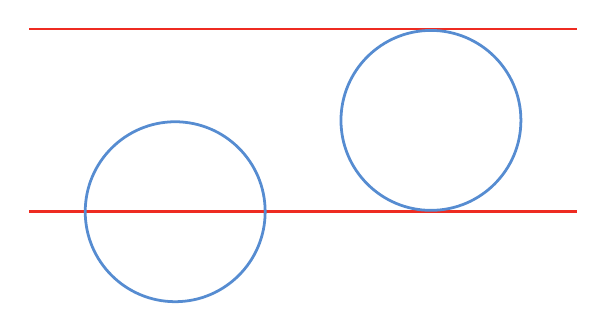
\begin{tikzpicture}[scale=0.58]
			\draw [toanhocdoisong, line width=1.pt] (-6.,6.)-- (6.,6.);
			\draw [toanhocdoisong, line width=1.pt] (-6.,10.)-- (6.,10.);
			\draw [cackithi, line width=1.pt] (2.8,8.) circle (1.97cm);
			\draw [cackithi, line width=1.pt] (-2.8,6.) circle (1.97cm);
		\end{tikzpicture}
		\caption{\small\textit{\color{toanhocdoisong}Hình $3$. Đường tròn có đường kính $d$ sẽ luôn cắt một đường kẻ tại hai điểm hoặc tiếp xúc hai đường kẻ.}}
		\vspace*{-10pt}
	\end{figure}
	Đường tròn có đường kính $d$ sẽ luôn cắt một đường kẻ tại $2$ giao điểm hoặc tiếp xúc với $2$ đường kẻ liên tiếp, do đó với đường tròn này $E=2$. Thay vào ($1$) ta có:
	\begin{align*}
		2=c\cdot\pi d
	\end{align*}
	hay $c = \dfrac{2}{\pi d}$.
	\vskip 0.1cm
	Vậy xác suất để một cây kim khi thả cắt đường nằm ngang trên giấy là 
	\begin{align*}
		P(l) = \frac{2l}{\pi d}. \tag{$2$}
	\end{align*}
	\begin{figure}[H]
		\vspace*{-5pt}
		\centering
		\captionsetup{labelformat= empty, justification=centering}
		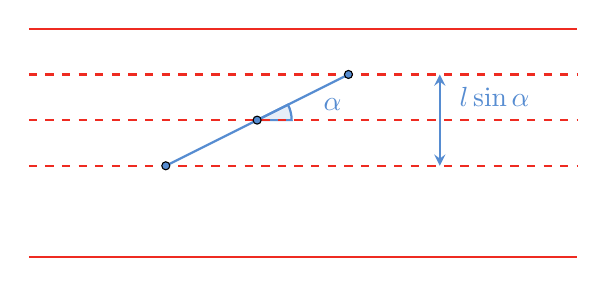
\begin{tikzpicture}[scale=0.58]
			\draw [shift={(-1.,8.)},line width=0.8pt,color=cackithi,fill=cackithi,fill opacity=0.15000000596046448] (0,0) -- (0.:0.7555063451882832) arc (0.:26.56505117707799:0.7555063451882832) -- cycle;
			\draw [toanhocdoisong,line width=0.8pt] (-6.,10.)-- (6.,10.);
			\draw [toanhocdoisong,dashed, line width=0.8pt] (-6.,9.)-- (6.,9.);
			\draw [toanhocdoisong,dashed, line width=0.8pt] (-6.,8.)-- (6.,8.);
			\draw [toanhocdoisong,dashed, line width=0.8pt] (-6.,7.)-- (6.,7.);
			\draw [toanhocdoisong, line width=0.8pt] (-6.,5.)-- (6.,5.);
			\draw [cackithi,line width=0.8pt] (-3.,7.)-- (1.,9.);
			\draw [fill=cackithi] (-3,7) circle (2.5pt);
			\draw [fill=cackithi] (1,9) circle (2.5pt);
			\draw [fill=cackithi] (-1,8) circle (2.5pt);
			\draw [cackithi,-stealth,line width=0.8pt] (3.,8.)-- (3.,9.);
			\draw [cackithi,-stealth,line width=0.8pt] (3.,8.)-- (3.,7.);
			
			\draw[color=cackithi] (0.65,8.347966297286694) node {$\color{cackithi}\alpha$};
			\draw[color=cackithi] (4.2,8.5) node {$\color{cackithi}l\sin\alpha$};
		\end{tikzpicture}
		\caption{\small\textit{\color{toanhocdoisong}Hình $4$. Chứng minh công thức $(2)$ sử dụng tích phân.}}
		\vspace*{-10pt}
	\end{figure}
	Ta cũng có thể thu được đáp án này bằng cách sử dụng tích phân. Cụ thể là ta xây dựng một mô hình xác suất cho vị trí rơi của cây kim. Gọi $\alpha$ $(0\le \alpha \le \dfrac{\pi}{2})$ là góc mà cây kim tạo với phương nằm ngang. Hình chiếu của nó theo phương vuông góc với các đường kẻ sẽ có độ dài $l\sin\alpha$, mà khoảng cách giữa hai đường kẻ là $d$, do đó xác suất để nó cắt một đường kẻ là $\dfrac{l\sin\alpha}{d}$. Coi phân bố của $\alpha$ là đều trên khoảng $[0,\dfrac{\pi}{2}]$, ta tính giá trị trung bình bằng cách lấy tích phân trên khoảng này rồi chia cho $\dfrac{\pi}{2}$ để thu được ($2$):
	\begin{align*}
		P(l) &= \frac{2}{\pi }\int_0^{\frac{\pi }{2}} {\frac{{l\sin \alpha }}{d}} d\alpha  = \frac{2}{\pi }\frac{l}{d}\left[ { - \cos \alpha } \right]|_0^{\frac{\pi }{2}}\\
		& = \frac{2}{\pi }\frac{l}{d}.
	\end{align*}
	Với cây kim có độ dài lớn hơn $d$, xác suất để nó cắt ít nhất một đường kẻ trong khoảng $\left[\arcsin\left(\dfrac{d}{l}, \dfrac{\pi}{2}\right)\right]$ sẽ luôn là $1$, do đó:
	\begin{align*}
		&P(l) \\
		= \,&\frac{2}{\pi }\left( {\int_0^{\arcsin \left( {\frac{d}{l}} \right)} {\frac{{l\sin \alpha }}{d} + } \int_{\arcsin \left( {\frac{d}{l}} \right)}^{\frac{\pi }{2}} {1d\alpha } } \right)\\
		=\,&1 \!\!+\!\! \frac{2}{\pi }\!\left( \!\!{\frac{l}{d}\!\!\left(\!\! {1 \!-\! \sqrt {\!\!1 \!-\! \frac{{{d^2}}}{{{l^2}}}} \!} \right) \!\!-\! \arcsin\! \frac{d}{l}}\! \right)\!\!.\tag{$3$}
	\end{align*}
	Bài toán này cũng được Laplace mở rộng cho trường hợp lưới trên tờ giấy là lưới chữ nhật và  tính xác suất để cây kim không cắt một đường kẻ dọc hay ngang nào. 
	\vskip 0.1cm
	Cũng chính Laplace đã đề xuất sử dụng thí nghiệm này để tính giá trị của số $\pi$. Đây cũng là khía cạnh được biết đến nhiều nhất về bài toán cây kim của Buffon. Thật vậy, nếu trong $M$ lần thả cây kim, ta thu được $m$ lần mà nó cắt một đường kẻ, công thức ($2$) cho ta:
	\begin{align*}
		\pi = \frac{2l}{d\cdot\left(\frac{m}{M}\right)},
	\end{align*}
	với $\dfrac{m}{M}$ là xác suất thực nghiệm của sự kiện cây kim cắt một đường kẻ.
	\vskip 0.1cm
	Đề xuất này của Laplace rất gần với phương pháp Monte Carlo của hơn một thế kỉ sau. Tuy vậy, về mặt thực tế, nó gập phải một số vấn đề. Nhiều thí nghiệm được tiến hành và cho kết quả của $\pi$ không quá chính xác: $3{,}1596$; $3{,}1553$; $3{,}137$.
	\vskip 0.1cm 
	Năm $1901$, Lazzarini công bố giá trị $3{,}1415929$ cho $3408$ lần thả cây kim, một giá trị khá chính xác (so với giá trị đã biết hiện nay, thì chỉ có chữ số cuối là không đúng). Tuy vậy, một số nghiên cứu đã chỉ ra kết quả này hầu như là ngụy tạo. Theo các lí thuyết về ước lượng tham số, để có độ chính xác đến $6$ chữ số sau dấu phẩy, cần phải tiến hành thí nghiệm trên $1{,}34×10^{14}$ lần chứ không phải vài nghìn lần. Đồng thời, số liệu của Lazzarini sử dụng phân số $\dfrac{355}{113}$, một số hữu tỉ được biết là một xấp xỉ tốt cho $\pi$. 
	\vskip 0.1cm
	Ngay cả với máy tính điện tử thì việc ước lượng $\pi$ bằng cách sử dụng thí nghiệm Buffon cũng không đạt được độ chính xác quá cao do việc làm tròn số trên máy tính. Đồng thời, các chữ số của $\pi$ cũng có thể được tính toán một cách chính xác hơn bởi các phương pháp khác.
	\vskip 0.1cm
	Tuy vậy, bài toán cây kim của Buffon có một ý nghĩa quan trọng trong lịch sử toán học bởi sự liên hệ giữa xác suất và hình học. Đây là một hướng tiếp cận mới khác với hướng tiếp cận xác suất sử dụng tổ hợp như truyền thống.
	\vskip 0.1cm
	\textbf{\color{toanhocdoisong}Bài tập}
	\vskip 0.1cm
	$1$. Chứng minh rằng khi cây kim vô cùng dài thì một cách hầu chắc chắn nó sẽ luôn cắt ít nhất một đường kẻ, tức là biểu thức trong ($3$) có giới hạn là $1$ khi $l\to \infty$.
	\vskip 0.1cm
	$2$. Trên tờ giấy với các đường kẻ ngang cách nhau khoảng $d$, thả ngẫu nhiên một đường tròn với bán kính $r < \dfrac{d}{2}$. Hãy tính xác suất để đường tròn cắt và không cắt các đường kẻ.
	\vskip 0.1cm
	$3$. Tương tự bài trên nhưng thả một hình vuông có cạnh $a<d$. Hãy tính xác suất để số giao điểm của các cạnh hình vuông với các đường kẻ ngang là:
	\vskip 0.1cm
	$a)$ $0$\quad\quad		$b)$ $1$\quad\quad		$c)$ $2$\quad\quad
	$d)$ $3$\quad\quad		$e)$ $4$
	\vskip 0.1cm
	Gợi ý: Xét trường hợp $a<\dfrac{d}{\sqrt{2}}$ và $a> \dfrac{d}{\sqrt{2}}$.
	\vskip 0.1cm	
	$4$. Trong thí nghiệm Buffon, với cây kim có độ dài $l>d$, hãy chứng minh giá trị kỳ vọng của số giao điểm của cây kim với các đường kẻ ngang là $E = \dfrac{2l}{\pi d}$. (Gợi ý: Gọi $N$ là số nguyên lớn nhất sao cho $d<\dfrac{l}{N}$, coi cây kim là hình gồm $N$ đoạn thẳng bằng nhau).
	\vskip 0.1cm
	$5$. Mở rộng của Laplace. Trên một lưới chữ nhật, với mỗi hình chữ nhật có chiều dài $a$ và chiều rộng $b$, thả ngẫu nhiên một cây kim chiều dài $l$ (biết rằng $l$ nhỏ hơn cả $a$ và $b$). Hãy tính xác suất để cây kim không chạm bất kỳ cạnh nào của lưới.
	\vskip 0.1cm
	$6$. Lưới Uspensky. Cho một lưới tam giác đều như hình vẽ với $d$ là chiều cao của mỗi tam giác đều. Thả một cây kim chiều dài \linebreak$l<d$ lên lưới tam giác đều này. Hãy tính xác suất để số giao điểm của cây kim với các đường trong lưới là:
	\vskip 0.1cm
	\quad\quad$a)$ $0$\quad\quad		$b)$ $1$\quad\quad		$c)$ $2$	\quad\quad	$d)$ $3$
	\begin{figure}[H]
		\vspace*{5pt}
		\centering
		\captionsetup{labelformat= empty, justification=centering}
		\includegraphics[width=1\linewidth]{6}
		\vspace*{-15pt}
	\end{figure}
	$7$. Bài toán sợi mì của Buffon. Trên một tờ giấy với các đường kẻ ngang song song cách nhau khoảng $d$, ném ngẫu nhiên một sợi mì ướt có độ dài $l$. Chứng minh rằng giá trị kì vọng của số giao điểm của sợi mì với các đường kẻ ngang là $E=\dfrac{2l}{\pi d}$. Giả sử rằng khi ném sợi mì, chiều dài của nó không đổi nhưng nó có thể uốn thành một đường cong bất kỳ.
	\vskip 0.1cm
	\textbf{\color{toanhocdoisong}$\pmb{2.}$ Đo độ dài bằng phương pháp ngẫu nhiên}
	\vskip 0.1cm
	Với một số thay đổi, thí nghiệm của Buffon có thể được sử dụng để giải quyết một vấn đề thực tế trong khoa học: đo độ dài của rễ cây (Newman, $1966$). Xét một bản thủy tinh mà trên đó một mẫu vật (ví dụ rễ cây) được trải phẳng. Khi quan sát mẫu vật qua kính hiển vi, người ta sử dụng một thị kính với một đường sợi tóc để soi các vùng khác nhau của bản thủy tinh.
	\vskip 0.1cm
	Với mỗi lần quan sát, thị kính được quay một góc bất kì và đường sợi tóc cũng được quay theo. Sau đó, số giao điểm của đường sợi tóc với rễ cây sẽ được ghi lại. Cách thức này được lặp lại nhiều lần với các vị trí quan sát ngẫu nhiên khác nhau trên bản thủy tinh. Để tiện lợi hơn, ta có thể đặt bản thủy tinh trên một tấm giấy với các điểm ngẫu nhiên đã được đánh dấu trước. Các điểm quan sát cũng có thể là một lưới ô vuông các điểm cách đều.
	\begin{figure}[H]
%		\vspace*{5pt}
		\centering
		\captionsetup{labelformat= empty, justification=centering}
		\includegraphics[width=1\linewidth]{7}
		\includegraphics[width=1\linewidth]{8}
		\caption{\small\textit{\color{toanhocdoisong}Hình $5$. Trên: Thị kính của kính hiển vi có đường sợi tóc (đường thẳng đứng). Dưới: minh họa phép đo độ dài rễ cây (màu xanh) với các vị trí và góc quay khác nhau của đường sợi tóc (màu đỏ). Số lượng đường sợi tóc trong hình chỉ mang tính minh họa, trong thực tế, cấu trúc rễ cây càng phức tạp thì số lượng đường sợi tóc cần sử dụng lại càng nhiều. Mỗi lần quan sát qua kính, ta chỉ thấy được một vùng hình tròn có đường kính là đường sợi tóc.}}
		\vspace*{-10pt}
	\end{figure}
	Về mặt bản chất, thay vì đếm số giao điểm của cây kim được thả ngẫu nhiên với các đường kẻ ngang, ta đếm số giao điểm của các đường sợi tóc được phân bố ngẫu nhiên với mẫu vật rễ cây (gồm nhiều đường cong) trên bản thủy tinh.
	\vskip 0.1cm
	Độ dài của rễ cây có thể được tính theo công thức:
	\begin{align*}
		R= \frac{\pi N A}{2H},	\tag{$4$}
	\end{align*}
	với $N$ là số giao điểm đã được đếm, $A$ là diện tích bản thủy tinh và $H$ là tổng độ dài của tất cả các đường sợi tóc.
	\vskip 0.1cm
	Thật vậy, xét một đoạn rễ cây $PQ$ có chiều dài $\Delta R$ và một đường sợi tóc $MN$ chiều dài $h$. Nếu khoảng cách từ trung điểm $D$ của $PQ$ đến $MN$ lớn hơn $\dfrac{1}{2}\Delta R$ thì $PQ$ và $MN$ chắc chắn không cắt nhau. Miền giới hạn này được biểu diễn bằng đường nét đứt trong hình. Giả sử $\dfrac{\Delta R}{h}$ là nhỏ, diện tích miền này có thể được xấp xỉ bằng $\Delta R \cdot h$. Do $MN$ được phân bố ngẫu nhiên trên bản thủy tinh, xác suất để $D$ nằm trong miền này là $\dfrac{\Delta R \cdot h}{A}$.
	\vskip 0.1cm
	Khi $D$ nằm trong miền cách $MN$ một khoảng không quá $\dfrac{1}{2}\Delta R$, khoảng cách từ $D$ đến $MN$ cần phải không lớn hơn $\dfrac{1}{2}\Delta R |\sin \theta |$, với $\theta$ là góc tạo bởi hai đường thẳng $PQ$ và $MN$, để $PQ$ và $MN$ cắt nhau. Xác suất để $PQ$ và $MN$ cắt nhau khi $D$ đã nằm trong miền trên là:
	\begin{align*}
		\frac{\frac{1}{2}\Delta R|\sin\theta|}{\frac{1}{2}\Delta R} = |\sin\theta|.
	\end{align*}
	Do đó, theo công thức nhân xác suất, xác suất để $PQ$ và $MN$ cắt nhau là:
	\begin{align*}
		p = \frac{\Delta R\cdot h}{A} |\sin\theta|.
	\end{align*}
	\begin{figure}[H]
		\vspace*{-5pt}
		\centering
		\captionsetup{labelformat= empty, justification=centering}
		\includegraphics[width=1\linewidth]{9}
		\caption{\small\textit{\color{toanhocdoisong}Hình $6$. Đoạn rễ cây $PQ$ và đường sợi tóc $MN$.}}
		\vspace*{-10pt}
	\end{figure}
	Tổng độ dài của các đoạn sợi tóc được phân bố ngẫu nhiên trên miền diện tích $A$ là $H$. Các góc $\theta$ cũng nhận giá trị ngẫu nhiên trong khoảng $[0,2\pi]$ nên giá trị kì vọng của số giao điểm của $PQ$ với các đường sợi tóc là:
	\begin{align*}
		\frac{1}{2\pi}\int_0^{2\pi}{\frac{{\Delta R \cdot H}}{A}}|\sin\theta|d\theta= \frac{2\left(\Delta R \cdot H\right)}{\pi A}.
	\end{align*}
	Coi rễ cây là một hình với nhiều đoạn có độ dài $\Delta R$, ta được giá trị kì vọng của số giao điểm của rễ cây với tất cả các đường sợi tóc là:
	\begin{align*}
		N = \frac{2RH}{\pi A}.
	\end{align*}
	Do $N$ là giá trị kỳ vọng nên khi đo đạc người ta cần phải tiến hành nhiều lần quan sát với các vị trí ngẫu nhiên của đường sợi tóc để kết quả thí nghiệm gần với giá trị của $N$ trong công thức.
	\vskip 0.1cm
	Ví dụ, với bản thủy tinh $10\times 20$ cm; tiến hành quan sát $40$ lần, độ dài đường sợi tóc (đường kính của thị trường vùng quan sát được) là $1{,}88$ cm; số giao điểm quan sát được là $344$ thì tổng độ dài của rễ cây là:
	\begin{align*}
		R - \frac{\pi \cdot 344\cdot 10 \cdot 20}{2\cdot40 \cdot1{,}88} = 1436 \text{ cm}.
	\end{align*}
	Cách đo độ dài này đã được các nhà thực vật học sử dụng trong nhiều thập kỉ mãi cho đến gần đây mới được thay thế bởi các phần mềm xử lí ảnh từ các camera có độ phân giải cao.
	\vskip 0.1cm
	\textbf{\color{toanhocdoisong}$\pmb{3.}$ Kiến biết đo diện tích bằng xác suất?}
	\vskip 0.1cm
	Phương pháp đo độ dài ở phần trước cũng có thể được biến đổi để tiến hành đo diện tích.
	\vskip 0.1cm
	Một nghiên cứu khá thú vị trên loài kiến \textit{Leptothorax albipennis} đưa ra giả thuyết rằng loài kiến này đã sử dụng xác suất để tính diện tích khi chọn tổ (kiến thường cố gắng chọn tổ có diện tích lớn nhất trong các vị trí khảo sát) (Mallon \& Franks, $2000$).
	\vskip 0.1cm
	Khi sử dụng camera để theo dõi kiến trinh sát trong phòng thí nghiệm, người ta thấy trong lần thứ nhất đến một vị trí để khảo sát, con kiến sẽ đi một cách ngẫu nhiên trong hộp theo một đường cong bao phủ phần lớn các vị trí trong hộp (gọi là đường cong $L$). Trong những lần tiếp theo (thường nó sẽ quay lại lần thứ hai hoặc có thể là lần thứ $3$), nó sẽ đi một đường cong đơn giản hơn (gọi là đường cong $S$). Đồng thời, khi đến các vị trí đã đi qua (kiến khi di chuyển có thể tiết ra pheromone để đánh dấu đường đi của mình), tức là các giao điểm của $L$ và $S$, kiến dành thời gian lâu hơn nhiều.
	\begin{figure}[H]
		\vspace*{-5pt}
		\centering
		\captionsetup{labelformat= empty, justification=centering}
		\includegraphics[width=0.65\linewidth]{10}
		\caption{\small\textit{\color{toanhocdoisong}Hình $7$. Từ trên xuống: Đường đi của kiến trinh sát khi khảo sát tổ được camera ghi lại trong lần khảo sát thứ nhất, thứ hai và thứ ba.}}
		\vspace*{-10pt}
	\end{figure}
	Theo các tác giả, số giao điểm của $L$ và $S$ được kiến trinh sát sử dụng để đánh giá diện tích của một vị trí làm tổ. Trong công thức ($4$), nếu ta thay các đường sợi tóc bằng một đường cong $L$ và rễ cây $R$ bằng đường cong $S$, công thức này vẫn đúng và diện tích có thể được xấp xỉ theo 
	\begin{align*}
		A = \frac{2SL}{\pi N}, \tag{$5$}
	\end{align*}
	với $N$ là số giao điểm của $S$ và $L$.
	\vskip 0.1cm
	Để kiểm chứng việc này, thí nghiệm được tiến hành với nhiều con kiến trinh sát khác nhau trên các loại hộp để làm tổ như trong hình vẽ.
	\vskip 0.1cm
	Trong thí nghiệm để chọn giữa hai tổ cùng chu vi (hình $8a$ và hình $8c$), kiến luôn chọn tổ có diện tích lớn hơn sau khi khảo sát cả hai. Do đó, diện tích chứ không phải chu vi mới là tiêu chí chọn tổ. Vì các tổ có một tấm chắn ở giữa (hình $8d$) cũng được chọn với khả năng tương tự như tổ bình thường, cho thấy số lần va chạm với chướng ngại vật trong tổ cũng không phải nhân tố quyết định.
	\begin{figure}[H]
		\vspace*{-5pt}
		\centering
		\captionsetup{labelformat= empty, justification=centering}
		\includegraphics[width=1\linewidth]{11}
		\caption{\small\textit{\color{toanhocdoisong}Hình $8$. Các loại tổ được sử dụng trong thí nghiệm về việc chọn tổ của kiến trinh sát. $a)$ tổ tiêu chuẩn; $b)$ tổ đồng dạng và có diện tích bằng một nửa tổ tiêu chuẩn; $c)$ tổ có diện tích bằng một nửa tổ tiêu chuẩn nhưng có cùng chu vi; $d)$ tổ tiêu chuẩn có tấm chắn ở giữa; $e)$ tổ dạng $b$ với một nửa được phủ các tấm đệm có thể nhấc ra.}}
		\vspace*{-10pt}
	\end{figure}
	Thí nghiệm cũng cho thấy khi kiến trở lại lần thứ hai, nếu tổ đã được thay bằng một tổ mới hoặc một tổ đã được một con kiến khác đi qua, nó sẽ tiến hành khảo sát lại như là đang đi qua lần thứ nhất. Điều này cho thấy trong lần khảo sát thứ nhất, kiến sẽ lưu lại pheromone đánh dấu đường đi và pheromone này đặc trưng cho từng cá thể. Việc này cũng cho phép các con kiến không làm ảnh hưởng đến quá trình khảo sát của nhau khi một vị trí có thể được nhiều hơn một con kiến đến thăm dò.
	\vskip 0.1cm
	Nếu kiến trở lại lần thứ ba hoặc sau đó, thời gian nó tiến hành khảo sát cũng không khác nhiều lắm so với lần thứ hai, do đó có thể thấy pheromone chỉ được rải ở lần thăm dò thứ nhất còn các lần lặp lại sau để tăng độ chính xác của việc ước lượng.
	\vskip 0.1cm
	Loại tổ trong hình $8e$ được thiết kế đồng dạng với tổ trong hình $8a$ nhưng có diện tích bằng một nửa. Đồng thời, ở nền của loại tổ này, một nửa diện tích là các tấm đệm có thể lấy ra. Sau khi kiến khảo sát tổ dạng này lần thứ nhất, người ta sẽ lấy các tấm đệm ra trước khi kiến quay lại lần thứ hai. Khi kiến trở lại, do các vị trí có đệm bị lấy ra không còn pheromone nên số giao điểm của đường đi của nó trong lần thứ hai với đường đi trong lần thứ nhất sẽ giảm một nửa. Trong thí nghiệm chọn giữa tổ dạng $8a$ và dạng $8e$, một nửa số kiến chọn $8e$ dù diện tích chỉ có một nửa. Thí nghiệm với kích thước tổ lớn gấp đôi cho thấy khoảng cách $L$ của mỗi con kiến là không đổi giữa các tổ với diện tích khác nhau. Kết hợp với với ($5$), có thể thấy thấy kiến đánh giá diện tích theo tỉ lệ nghịch với tần số gặp giao điểm $\dfrac{N}{S}$.
	\vskip 0.1cm
	Việc nghiên cứu những thuật toán liên quan đến hành vi của kiến không chỉ có ý nghĩa về mặt sinh học mà còn có nhiều ứng dụng khác, ví dụ như trong việc lập trình điều khiển hành vi của robot.
	\vskip 0.1cm
	$\pmb{4.}$ \textbf{\color{toanhocdoisong}Lời kết}
	\vskip 0.1cm
	Lĩnh vực xác suất hình học còn có nhiều bài toán khác có giá trị về cả mặt lý thuyết lẫn thực tiễn. Pi cũng sẽ tiếp tục giới thiệu các bài toán này đến với độc giả trong tương lai không xa.
	\vskip 0.1cm
	\textbf{\color{toanhocdoisong}Tài liệu tham khảo}
	\vskip 0.1cm
	[$1$] Aigner, M., \& Ziegler, G. ($2004$). \textit{Proof from} THE BOOK. Springer--Verlag.
	\vskip 0.1cm
	[$2$] Mallon, E. B., \& Franks, N. R. ($2000$). Ants estimate area using Buffon's needle. \textit{Proc. R. Soc. Lond.} B($267$), $765-770$.
	\vskip 0.1cm
	[$3$] Mugford, S. T., Mallon, E. B., \& Franks, N. R. ($2001$). The accuracy of Buffon's needle: a rule of thumb used by ants to estimate area. \textit{Behavioral Ecology}, $12(6)$, $655-658$.
	\vskip 0.1cm
	[$4$] Newman, E. I. ($1966$). A Method of Estimating the Total Length of Root in a Sample. \textit{Journal of Applied Ecology}, $139-145$.
	\vskip 0.1cm
	[$5$] Ramaley, J. F. ($1969$). Buffon's Noodle Problem. \textit{The American Mathematical Monthly}, $78(8)$, $916-918$.
\end{multicols}
%	\newpage

%	 
%	 \setcounter{figure}{0}
%	 \thispagestyle{hoccungpinone}
\pagestyle{hoccungpi}
\everymath{\color{hoccungpi}}
\graphicspath{{../hoccungpi/pic/}}
\blfootnote{$^{1}$\color[named]{hoccungpi}THPT chuyên Nguyễn Quang Diêu -- Đồng Tháp.}
\begingroup
\AddToShipoutPicture*{\put(0,616){\includegraphics[width=19.3cm]{../bannerhoccungpi}}}
\AddToShipoutPicture*{\put(98,522){\includegraphics[scale=1]{../tieude1.pdf}}}
\centering
\endgroup
\vspace*{188pt}

\begin{multicols}{2}
		\textbf{\color{hoccungpi}Giới thiệu}
		\vskip 0.1cm
		Trong tạp chí Pi tháng $10$ năm $2021$, tác giả Trần Nam Dũng  giới thiệu đến bất đẳng thức Bernoulli, ở đó tác giả có đề cập đến việc bất đẳng thức Cauchy (hay còn gọi là bất đẳng thức trung bình cộng và trung bình nhân) tương đương với bất đẳng thức Bernoulli. Bài viết này sẽ tổng hợp nhiều hơn các bất đẳng thức tương đương như vậy cũng như một số chứng minh đặc sắc có liên quan. Bài viết kết thúc với một số bài toán xuất hiện trong các kỳ thi Olympic mà ở đó bất đẳng thức Bernoulli có vai trò then chốt trong lời giải.
		\vskip 0.1cm
		$\pmb{1.}$ \textbf{\color{hoccungpi}Một số bất đẳng thức tương đương với bất đẳng thức Bernoulli}
		\vskip 0.1cm
		Nhắc lại rằng bất đẳng thức Bernoulli cho số mũ thực được phát biểu như sau (xem [$1$, Định lý $2$]: Cho số thực $x > -1$ và số thực $\alpha$. Khi đó, 
		\vskip 0.1cm
		$(1)$ Với $0 < \alpha < 1$, ta có  $(1+x)^\alpha \le 1 + \alpha x$.
		\vskip 0.1cm
		$(2)$ Với  $\alpha > 1$ hoặc $\alpha < 0$, ta có  $(1+x)^\alpha \ge 1 + \alpha x$.
		\vskip 0.1cm
		Dấu ``$=$" xảy ra khi và chỉ khi $x = 0$.
		\vskip 0.1cm
		Chúng ta sẽ bắt đầu với  kết quả sau đây.
		\vskip 0.1cm
		\textbf{\color{hoccungpi}Định lý} $\pmb{1.}$ \textit{Các mệnh đề sau là tương đương:
		\vskip 0.1cm
		$(a)$ Với $x>-1$ và $\alpha \in (0;1)$ thì $(1+x)^{\alpha} \le 1+\alpha x.$
		\vskip 0.1cm
		$(b)$ Với mọi số thực dương $\alpha, x,y$, trong đó $\alpha \in (0;1)$, ta có
		$x^{\alpha}y^{1-\alpha} \le \alpha x +(1-\alpha)y.$
		\vskip 0.1cm
		$(c)$ Hàm số $y=\ln x$ là hàm lõm trên $(0;+\infty)$. (Ở đây, ta nói một hàm số $f$ trên khoảng $I$ là lõm nếu với mọi $x, y\in I$ và $\alpha \in (0, 1)$ thì $f(\alpha x+(1-\alpha) y) \ge \alpha f(x) + (1-\alpha)f(y)$.\footnote[2]{\color{hoccungpi}Lưu ý rằng định nghĩa này khác với một số tài liệu, trong đó hàm số như vậy được gọi là lồi!})
		\vskip 0.1cm
		$(d)$ (Bất đẳng thức Young.) Với $x,y,p,q$ là các số thực dương thỏa mãn
		$\dfrac{1}{p}+\dfrac{1}{q}=1$ thì 
		\begin{align*}
			xy \le \dfrac{x^{p}}{p}+\dfrac{y^{q}}{q}.
		\end{align*}}
		\textit{Chứng minh.}
		\setlength{\abovedisplayskip}{7.2pt}
		\setlength{\belowdisplayskip}{7.2pt}
		\vskip 0.1cm
		$\bullet$ $(a) \Rightarrow (b)$.  Thay $x+1$ bằng $x$ vào bất đẳng thức (a) ta có $x^{\alpha} \le 1+\alpha(x-1)$, hay 
		\begin{align*}
			x^{\alpha} \le (1-\alpha) + \alpha x
		\end{align*}
		với mọi $ x>0,\alpha \in (0;1)$. Nhân cả hai vế của bất đẳng thức vừa nhận được với số thực dương $y$ ta được:
		\begin{align*}
			x^{\alpha}y \le (1-\alpha)y + \alpha xy.
		\end{align*}
		(Bất đẳng thức này đúng với mọi $x>0, y>0, \alpha \in (0;1)$.) Thay $x$ bằng $\dfrac{x}{y}$ vào bất đẳng thức này, ta thu được:
		\begin{align*}
			x^{\alpha}y^{1-\alpha} \le (1-\alpha)y + \alpha x,
		\end{align*}
		nghĩa là bất đẳng thức $(b)$ là đúng.
		\vskip 0.1cm
		$\bullet$ $(b) \Rightarrow (c)$ Sử dụng định nghĩa của hàm lõm.
		\vskip 0.1cm
		$\bullet$ $(c) \Rightarrow (d)$. Vì $y=\ln x$ là hàm lõm nên:
		\begin{align*}
			\ln \left( {\frac{1}{p}{x^p} + \frac{1}{q}{y^q}} \right) \ge   \frac{1}{p}\ln {x^p} + \frac{1}{q}\ln {x^q},
		\end{align*}
		do đó
		\begin{align*}
			\frac{{{x^p}}}{p} + \frac{{{y^q}}}{q} \ge xy,
		\end{align*}
		hay nói cách khác, $(d)$ đúng.
		\vskip 0.1cm
		$\bullet$ $(d) \Rightarrow (a)$. Xét $\alpha \in (0;1)$. Khi đó tồn tại số thực $p>1$ sao cho $\dfrac{1}{p}=\alpha$. Đặt $1-\alpha=\dfrac{1}{q}$ (như vậy $q>1$). Thay $x, y$ tương ứng bởi $x^p, y^q$ vào bất đẳng thức Young ta nhận được
		\begin{align*}
			x^{\alpha}y^{1-\alpha} \le \alpha x + (1-\alpha)y.
		\end{align*}
		Bất đẳng thức này đúng với mọi số thực $ x,y>0,\alpha \in (0;1)$. Đặc biệt, với $y=1$ ta được:
		\begin{align*}
			x^{\alpha} \le \alpha x + (1-\alpha),
		\end{align*}
		với mọi $x,\alpha \in (0;1)$, hay nói cách khác:
		\begin{align*}
			x^{\alpha} \le 1+\alpha (x-1).
		\end{align*}
		Thay $x$ bằng $x+1$, ta thu được:
		\begin{align*}
			(x+1)^{\alpha} \le 1+\alpha x
		\end{align*}
		với mọi $x>-1,\alpha \in (0;1)$. Vậy $(a)$ đúng.
		\vskip 0.1cm
		Tóm lại
			$(a) \Leftrightarrow (b) \Leftrightarrow (c) \Leftrightarrow (d).$
		\vskip 0.1cm
		Tiếp theo, tác giả xin trình bày một mạch tương đương dài hơn giữa nhiều bất đẳng thức quen thuộc với bất đẳng thức Bernoulli.
		\vskip 0.1cm
		\textbf{\color{hoccungpi}Định lý} $\pmb{2.}$
		\textit{Các mệnh đề sau là tương đương:
		\vskip 0.1cm
		$(T_1)$: Với $x>-1,\alpha \geq 1$ thì $(1+x)^{\alpha} \geq 1+\alpha x.$
		\vskip 0.1cm
		$(T_2)$: Với $x>-1,\alpha \leq 0$ thì
		$(1+x)^{\alpha} \geq 1+\alpha x.$
		\vskip 0.1cm
		$(T_3)$: Với $x>-1,0 \le \alpha \le 1$ thì
		$(1+x)^{\alpha} \le 1+\alpha x.$
		\vskip 0.1cm
		$(T_4)$: Với mọi số nguyên dương $n$ và các số thực $a_i,q_i>0$ ($1\le i \le n$), $ \alpha \geq 1$ thỏa mãn  $\sum_{i=1}^n q_i=1$ thì
		\begin{align*}
			\sum_{i=1}^n q_i a_i^{\alpha} \leq \left(\sum_{i=1}^n q_i a_i
			\right)^{\alpha}.
		\end{align*}
		$(T_5)$: Với mọi số nguyên dương $n$ và các số thực$a_i,q_i>0$ ($1\le i \le n$), $ \alpha \geq 1$ thỏa  mãn  $\sum_{i=1}^n q_i=1$ thì
		\begin{align*}
			\sum_{i=1}^n q_i a_i^{\alpha} \geq \left(\sum_{i=1}^n q_i a_i
			\right)^{\alpha}.
		\end{align*}
		$(T_6)$: Với mọi số nguyên dương $n$ và các số thực dương $a_i,p_i$ ($1\le i \le n$), định nghĩa $M_r$ ($r>0$) như sau:
		\begin{align*}
			M_{r}\!=\!\begin{cases}
				\!\!\left(\dfrac{p_{1} a_{1}^{r}+p_{2} a_{2}^{r}+\ldots+p_{n} a_{n}^{r}}{p_{1}+p_{2}+\ldots+p_{n}}\right)^{\frac{1}{r}}\!\!\!\!, r \neq 0 \\[+1ex]
				\left(a_{1}^{p_{1}} a_{2}^{p_{2}} \cdots a_{n}^{p_{n}}\right)^{\frac{1}{p_{1}+p_{2}+\cdots+p_{n}}}, r=0
			\end{cases}
		\end{align*}
		Khi đó, với mọi $r<s$ thì
		\begin{align*}
			M_{r} \leq M_{s}.
		\end{align*}
		$(T_7)$: (Bất đẳng thức Holder.) Với mọi số nguyên dương $n$ và các số thực dương $a_i,b_i$ ($1\le i \le n$), $p,q$ thỏa mãn $\dfrac{1}{p}+\dfrac{1}{q}=1.$ Khi đó:
		\begin{align*}
			\sum_{i=1}^{n} a_{i} b_{i} \leq\left(\sum_{i=1}^{n} a_{i}^{p}\right)^{\frac{1}{p}}\left(\sum_{i=1}^{n} b_{i}^{q}\right)^{\frac{1}{q}}.
		\end{align*}
		$(T_8)$: (Bất đẳng thức Cauchy--Schwarz.) Với mọi số nguyên dương $n$ và các số thực dương $a_i,b_i$ ($1\le i \le n$) thì
		\begin{align*}
			\left(\sum_{i=1}^{n} a_{i} b_{i}\right)^{2} \leq\left(\sum_{i=1}^{n} a_{i}^{2}\right)\left(\sum_{i=1}^{n} b_{i}^{2}\right).
		\end{align*}
		$(T_{9})$: Với mọi số thực dương $a,b$,
		\begin{align*}
			\dfrac{1}{2}\ln a+\dfrac{1}{2}\ln b \le \ln \left(\dfrac{a+b}{2} \right).
		\end{align*}
		$(T_{10})$: Với mọi số nguyên dương $n$ và các số thực dương $a_i,p_i$ ($1\le i \le n$) thì
		\begin{align*}
			\dfrac{\sum_{i=1}^n p_i\ln a_i}{\sum_{i=1}^n p_i} \le \ln \left(\dfrac{ \sum_{i=1}^n p_ia_i}{\sum_{i=1}^n p_i} \right).
		\end{align*}
		$(T_{11})$: Với mọi số nguyên dương $n$ và các số thực dương $a_i,p_i$ ($1\le i \le n$) thì
		\begin{align*}
			\prod_{i=1}^{n} a_{i}^{\frac{p_{i}}{\sum_{k=1}^{n} p_{k}}} \leq \dfrac{\sum_{i=1}^{n} p_{i} a_{i}}{\sum_{k=1}^{n} p_{k}}.
		\end{align*}
		$(T_{12})$:  Với mọi số nguyên dương $m, n$ và các số thực
		dương $\alpha_{j}, \beta_{i}$ $(1\le i \le n, 1\le j \le m$) thỏa mãn $\sum_{j=1}^{n} \alpha_{j}=\sum_{i=1}^{m} \beta_{i}=1$, định nghĩa
		\begin{align*}
			&G_{i}=a_{i,1}^{\alpha_{1}} a_{i, 2}^{\alpha_{2}} \cdots a_{i,n}^{\alpha_{n}} \\
			\text{và } &A_{j}=\beta_{1} a_{1,j}+\beta_{2} a_{2,j}+\cdots+\beta_{m} a_{m,j},
		\end{align*}
		(với $i=1,2, \ldots, m$; $j=1,2, \ldots, n$ và \linebreak$a_{k,l}>0$).
		Khi đó:
		\begin{align*}
			\sum_{i=1}^{m} \beta_{i} G_{i} \leq \prod_{j=1}^{n} A_{j}^{\alpha_{j}}.
		\end{align*}
		$(T_{13})$: Với mọi số nguyên dương $m, n$ và $a_{i,j}$, ($1\le i\le m, 1\le j \le n$), $\alpha_k$, ($1\le k \le n$) là các số thực dương thỏa mãn $\sum_{i=1}^n \alpha_i=1$, ta~có
		\begin{align*}
			&\sum_{i=1}^{m} a_{i, 1}^{\alpha_{1}} a_{i, 2}^{\alpha_{2}} \cdots a_{i, n}^{\alpha_{n}} \\
			\leq &\prod_{j=1}^{n}\left(a_{1, j}+a_{2,j}+\cdots+a_{m, j}\right)^{\alpha_{j}}.
		\end{align*}
		$(T_{14})$: Với mọi số nguyên $m,n \geq 2$ và các số thực dương $a_{i, j}$ ($1\le i \le m, 1\le j \le n$), đặt
		\begin{align*}
			&A_{j}=\frac{1}{m} \sum_{i=1}^{m} a_{i,j}, G_{i}=\left(\prod_{j=1}^{n} a_{i,j}\right)^{\frac{1}{n}} \\
			&(1\le j \le n, 1\le i \le m).
		\end{align*} 
		Khi đó,
		\begin{align*}
			\sqrt[n]{A_{1} A_{2} \cdots A_{n}} \geq \frac{G_{1}+G_{2}+\cdots+G_{m}}{m}.
		\end{align*}
		$(T_{15})$: (Bất đẳng thức trung bình cộng và trung bình nhân.) Với mọi số nguyên dương $n$ và các số thực dương $a_i$ ($1\le i \le n$), ta có:
		\begin{align*}
			A_{n}\!=\!\frac{a_{1}\!+\!a_{2}\!+\!\cdots\!+\!a_{n}}{ n} \!\geq\! \sqrt[n]{a_{1} a_{2} \cdots a_{n}}\!=\!G_{n}.
		\end{align*}
		$(T_{16})$: Với mọi số thực dương $a,b$ là các số thực và số hữu tỷ $r \in (0;1)$, ta có:
		\begin{align*}
			a^{r} b^{1-r} \leq r a+(1-r) b.
		\end{align*}
		$(T_{17})$: Với mọi số thực $x \geq 0$ và số nguyên dương $n$,}
		\begin{align*}
			x-1 \geq n\left(x^{\frac{1}{n}}-1\right).
		\end{align*}
		\textit{Chứng minh.}
		Sơ đồ chứng minh:
		\begin{figure}[H]
			\vspace*{-5pt}
			\centering
			\captionsetup{labelformat= empty, justification=centering}
			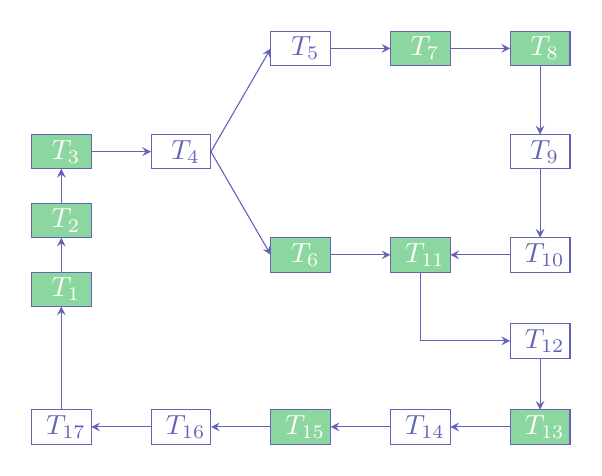
\begin{tikzpicture}[scale=0.38,yscale=1.15]
				%\draw (1,1) grid (19,13);
				\draw[hoccungpi](1,1) rectangle (3,2);
				\draw[hoccungpi](2,1.5) node[] {{ $T_{17}$}};
				\fill[diendantoanhoc!60] (1,5) rectangle (3,6);
				\draw[hoccungpi] (1,5) rectangle (3,6);
				\draw[hoccungpi](2,5.5) node[white] {{ $T_{1}$}};
				\fill[diendantoanhoc!60](1,7) rectangle (3,8);
				\draw[hoccungpi](1,7) rectangle (3,8);
				\draw[hoccungpi](2,7.5) node[white] {{ $T_{2}$}};
				\fill[diendantoanhoc!60] (1,9) rectangle (3,10);
				\draw[hoccungpi] (1,9) rectangle (3,10);
				\draw[hoccungpi] (1,9) rectangle (3,10);
				\draw[hoccungpi](2,9.5) node[white] {{ $T_{3}$}};
				\draw[hoccungpi](5,9) rectangle (7,10);
				\draw[hoccungpi](6,9.5) node[] {{ $T_{4}$}};
				\draw[hoccungpi](5,1) rectangle (7,2);
				\draw[hoccungpi](6,1.5) node[] {{ $T_{16}$}};
				\fill[diendantoanhoc!60](9,1) rectangle (11,2);
				\draw[hoccungpi](9,1) rectangle (11,2);
				\draw[hoccungpi](10,1.5) node[white] {{ $T_{15}$}};
				\fill[diendantoanhoc!60] (9,6) rectangle (11,7);
				\draw[hoccungpi] (9,6) rectangle (11,7);
				\draw[hoccungpi](10,6.5) node[white] {{ $T_{6}$}};
				\draw[hoccungpi](9,12) rectangle (11,13);
				\draw[hoccungpi](10,12.5) node[] {{ $T_{5}$}};
				\draw[hoccungpi](13,1) rectangle (15,2);
				\draw[hoccungpi](14,1.5) node[] {{ $T_{14}$}};
				\draw[hoccungpi] (13,6) rectangle (15,7);
				\fill[diendantoanhoc!60] (13,6) rectangle (15,7);
				\draw[hoccungpi] (13,6) rectangle (15,7);
				\draw[hoccungpi](14,6.5) node[white] {{ $T_{11}$}};
				\fill[diendantoanhoc!60] (13,12) rectangle (15,13);
				\draw[hoccungpi] (13,12) rectangle (15,13);
				\draw[hoccungpi](14,12.5) node[white] {{ $T_{7}$}};
				\fill[diendantoanhoc!60] (17,12) rectangle (19,13);
				\draw[hoccungpi] (17,12) rectangle (19,13);
				\draw[hoccungpi](18,12.5) node[white] {{ $T_{8}$}};
				\draw[hoccungpi](17,9) rectangle (19,10);
				\draw[hoccungpi](18,9.5) node[] {{ $T_{9}$}};
				\draw[hoccungpi](17,6) rectangle (19,7);
				\draw[hoccungpi](18,6.5) node[] {{ $T_{10}$}};
				\draw[hoccungpi](17,3.5) rectangle (19,4.5);
				\draw[hoccungpi](18,4) node[] {{ $T_{12}$}};
				\fill[diendantoanhoc!60] (17,1) rectangle (19,2);
				\draw[hoccungpi] (17,1) rectangle (19,2);
				\draw[hoccungpi](18,1.5) node[white] {{ $T_{13}$}};
				\draw[hoccungpi,-stealth] (2,2) -- (2,5);
				\draw[hoccungpi,-stealth] (2,6) -- (2,7);
				\draw[hoccungpi,-stealth] (2,8) -- (2,9);
				\draw[hoccungpi,-stealth] (3,9.5) -- (5,9.5);
				\draw[hoccungpi,-stealth] (7,9.5) -- (9,12.5);
				\draw[hoccungpi,-stealth] (7,9.5) -- (9,6.5);
				\draw[hoccungpi,-stealth] (11,12.5) -- (13,12.5);
				\draw[hoccungpi,-stealth] (11,6.5) -- (13,6.5);
				\draw[hoccungpi,-stealth] (15,12.5) -- (17,12.5);
				\draw[hoccungpi,-stealth] (18,12) -- (18,10);
				\draw[hoccungpi,-stealth] (18,9) -- (18,7);
				\draw[hoccungpi,-stealth] (17,6.5) -- (15,6.5);
				\draw[hoccungpi,-stealth] (14,6) --(14,4)-- (17,4);
				\draw[hoccungpi,-stealth] (18,3.5) -- (18,2);
				\draw[hoccungpi,-stealth] (17,1.5) -- (15,1.5);
				\draw[hoccungpi,-stealth] (13,1.5) -- (11,1.5);
				\draw[hoccungpi,-stealth] (9,1.5) -- (7,1.5);
				\draw[hoccungpi,-stealth] (5,1.5) -- (3,1.5);
			\end{tikzpicture}
			\caption{\small\textit{\color{hoccungpi}(Các mệnh đề $T_i$ được tô màu xanh là các bất đẳng thức cổ điển, thường được sử dụng.)}}
			\vspace*{-10pt}
		\end{figure}
		Bạn đọc có thể thử sức mình bằng cách tự chứng minh các mũi tên $(T_i)\Rightarrow (T_{j})$ trong sơ đồ trên hoặc tham khảo bài viết [$2$]. (Bạn đọc sẽ tìm thấy trong tài liệu đã dẫn một mạch dài hơn của các bất đẳng thức tương đương với bất đẳng thức Bernoulli). Dưới đây, để minh họa, người viết chỉ điểm qua chứng minh mũi tên $(T_{17}) \Rightarrow (T_{1}).$  Xét số nguyên dương $n$ và số thực $x>0$. Ta có:
		\begin{align*}
			&\dfrac{{{x^{n + 1}} - 1}}{{n + 1}} - \dfrac{{{x^n} - 1}}{n} \\
			= &\dfrac{{x - 1}}{{n(n + 1)}}\left( {n{x^n} - {x^{n - 1}} - {x^{n - 2}} -  \ldots  - 1} \right)\\
			= &\dfrac{{{{(x - 1)}^2}}}{{n(n + 1)}}\left[ {x^{n - 1}} + \left( {{x^{n - 1}} + {x^{n - 2}}} \right) +  \ldots \right. \\
			& \left.+ \left( {{x^{n - 1}} + {x^{n - 2}} +  \ldots  + 1} \right) \right].
		\end{align*}
		Hệ thức trên đây, kết hợp với lập luận bằng quy nạp, dẫn đến
		\begin{align*}
			\frac{{{x^m} - 1}}{m} \geq \frac{{{x^n} - 1}}{n},
		\end{align*}
		với mọi số nguyên dương $m \geq n$. Thay $x^n$ bằng $x$ và $r= \frac{n}{m}$ vào bất đẳng thức vừa thu được, ta có
		\begin{align*}
			{x^r} - 1 \geq  r\left( {x - 1} \right).
		\end{align*}
		Bất đẳng thứuc này đúng với mọi số hữu tỷ $r \geq 1$ và  số thực $x>0$. Lại vì tập các số hữu tỷ
		lớn hơn hoặc bằng $1$ trù mật trong tập các số thực lớn hơn hoặc bằng $1$ nên ta có thể kết luận rằng
		\begin{align*}
			{x^{\alpha} } - 1 \geq  \alpha \left( {x - 1} \right)
		\end{align*}
		với mọi số thực $\alpha \geq 1,x>0$. Thay $x$ bởi $x+1$ ta có bất đẳng thức $(T_1)$. 
		\vskip 0.1cm
		$\pmb{2.}$ \textbf{\color{hoccungpi}Nét đẹp qua phép chứng minh}
		\vskip 0.1cm
		Một lời giải hay, đáng học hỏi chưa hẳn là một lời giải ngắn gọn. Bởi vì điểm hay có thể đến từ ý tưởng hoặc từ kỹ thuật xử lý bài toán (kéo theo là lời giải có thể tương đối dài hoặc không đơn giản). Trong mục này, mời bạn đọc đến với những lời giải như vậy.
		\vskip 0.1cm
		\textbf{\color{hoccungpi}Ví dụ} $\pmb{1.}$
		\textit{Ta nhắc lại hai bất đẳng thức sau:
		\vskip 0.1cm
		$\bullet$ \textbf{\color{hoccungpi}(AM -- GM)} Với mọi số thực dương $a_1, a_2, \ldots, a_n$, ta có
		\begin{align*}
			\dfrac{a_1+a_2+\cdots+a_n}{n} \geq \sqrt[n]{a_1a_2\cdots a_n}.
		\end{align*}
		$\bullet$ \textbf{\color{hoccungpi}(Bất đẳng thức Bernoulli cơ bản)} Với mọi số tự nhiên $n$ và số thực dương $x$, ta có
		\begin{align*}
			x^n \geq 1+n(x-1).
		\end{align*}	
		$a)$ Sử dụng bất đẳng thức AM -- GM, hãy chứng minh bất đẳng thức Bernoulli cơ bản.
		\vskip 0.1cm
		$b)$ Sử dụng bất đẳng thức Bernoulli cơ bản, hãy chứng minh bất đẳng thức AM -- GM.}
		\vskip 0.1cm
		\textit{Lời giải.}
		$a)$ Với $n=0,1$ thì bất đẳng thức Bernoulli cơ bản là hiển nhiên vì nó trở thành đẳng thức. Giả sử $n \geq 2$. Ta xét hai trường hợp 
		\vskip 0.1cm
		$\bullet$ Với $0<x \le 1-\dfrac{1}{n}$ thì bất đẳng thức là hiển nhiên do vế trái dương trong khi vế phải không dương.
		\vskip 0.1cm
		$\bullet$ Với $x>1-\dfrac{1}{n}$, áp dụng bất đẳng thức AM -- GM, ta có
		\begin{align*}
			{x^n}{\rm{ }} &= {\left\{ {\frac{{[1 + n(x - 1)] + \overbrace {1 +  \ldots  + 1}^{n - 1}}}{n}} \right\}^n} \\
			&\ge [1 + n(x - 1)] \cdot 1 \cdot  \ldots  \cdot 1 = 1 \!+\! n(x \!-\! 1).
		\end{align*}
		Ta chứng minh xong bất đẳng thức Bernoulli cơ bản.
		\vskip 0.1cm	
		$b)$ Đặt
		\begin{align*}
			A_n=\dfrac{a_1+a_2+\cdots+a_n}{n},
		\end{align*}
		trong đó $a_1, a_2, \ldots$ là các số thực dương. 
		Trước hết, với $n=1$ thì bất đẳng thức cần chứng minh là tầm thường 
		Xét trường hợp $n \geq 2$. Áp dụng bất đẳng thức Bernoulli, ta có
		\begin{align*}
			\left(\frac{A_{n}}{A_{n-1}}\right)^{n} & \geq 1+n\left(\frac{A_{n}}{A_{n-1}}-1\right) \\
			&=\frac{A_{n-1}+n A_{n}-n A_{n-1}}{A_{n-1}} \\
			&=\frac{n A_{n}-(n-1) A_{n-1}}{A_{n-1}}=\frac{a_{n}}{A_{n-1}}.
		\end{align*}
		Hay nói cách khác,
		\begin{align*}
			A_{n}^{n} \geq a_{n} \cdot A_{n-1}^{n-1}.
		\end{align*}		
		Áp dụng liên tục các bất đẳng thức như vậy, ta thu được
		\begin{align*}
			A_{n}^{n}  &\geq a_{n} \cdot A_{n-1}^{n-1} \geq a_{n} \cdot a_{n-1} \cdot A_{n-2}^{n-2}  \\
			&\geq \cdots \geq a_{n} \cdot a_{n-1} \cdots a_{3} \cdot A_{2}^{2} \\
			&\geq a_{n} \cdot a_{n-1} \cdots a_{3} \cdot a_2 \cdot a_1.
		\end{align*}
		Thế nhưng bất đẳng thức $A_n^n \geq a_1a_2 \cdots a_n$ tương đương với $\dfrac{a_1+a_2+\cdots+a_n}{n} \geq \sqrt[n]{a_1a_2\cdots a_n}$ nên bất đẳng thức AM -- GM được chứng minh.
		\vskip 0.1cm
		\textbf{\color{hoccungpi}Ví dụ} $\pmb{2.}$ \textit{Cho số thực $x>-1$ và số nguyên $k$. Chứng minh rằng $(1+x)^{k} \geq 1+ k x.$}
		\vskip 0.1cm
		 Lưu ý: trong ví dụ trên, số nguyên $k$ có thể âm.
		\vskip 0.1cm
		Với mỗi $x>-1$ cố định, ta xét hàm $\mathscr{B}$  sau đây:
		\begin{align*}
			\mathscr{B}: \mathbb{Z} & \rightarrow \mathbb{R} \\
			k&  \mapsto (1+x)^{-k}(1+k x).
		\end{align*}
		Có thể thấy rằng  $\mathscr{B}(0)= \mathscr{B}(1)=1$. 
		Ta sẽ chứng minh $1$ cũng chính là giá trị lớn nhất của $\mathscr{B}$, từ đó ta thu được kết luận của bài toán. Ta có
		\begin{align*}
			&\mathscr{B}(k)-\mathscr{B}(k-1) \\
			=&\frac{1+k x}{(1+x)^{k}}-\frac{1+(k-1) x}{(1+x)^{k-1}} \\
			=&\frac{1\!+\!k x\!-\![1\!+\!(k\!-\!1) x](1\!+\!x)}{(1\!+\!x)^{k}}=\frac{(1-k) x^{2}}{(1+x)^{k}}.
		\end{align*}
		Vì thế $\mathscr{B}(k)-\mathscr{B}(k-1) \ge 0$ nếu $k\le 0$ và $\mathscr{B}(k)-\mathscr{B}(k-1) \le 0$ nếu $k\ge 2$.
		Ta suy ra giá trị lớn nhất của
		$\mathscr{B}$ là $1$ và do đó chứng minh hoàn tất.
		\vskip 0.1cm
		\textbf{\color{hoccungpi}Ví dụ $\pmb{3.}$ (Bất đẳng thức Bernoulli cho số mũ nằm trong khoảng $\pmb{(0;1)}$).}
		\textit{Cho các số thực $x>-1$ và $0<\alpha <1$. Chứng minh rằng}
			$(1+x)^{\alpha} \le 1+ \alpha x.$
		\vskip 0.1cm
		\textit{Lời giải.} Ta xét tập hợp $T$ sau đây:
		\begin{align*}
			&T=\{\alpha \in (0;1): \forall \,\,y>-1 \\
			&\textrm{ thì } (1+y)^{\alpha} \le 1+ \alpha y\}.
		\end{align*}
		Trước tiên, ta sẽ chứng minh $T$ có ba tính chất sau:
		\vskip 0.1cm
		$(1)$ $\dfrac{1}{2} \in T$.
		\vskip 0.1cm
		$(2)$ Nếu $\alpha \in T$ thì $1-\alpha \in T$.
		\vskip 0.1cm
		$(3)$ Nếu $\alpha, \beta \in T$ thì $\alpha \beta \in T$. Hơn nữa, nếu $\alpha + \beta<1$ thì $\alpha + \beta\in T$.
		\vskip 0.1cm
		Thật vậy,
		\vskip 0.1cm 
		$(1)$ Trước hết ta thấy rằng $\left(1+\frac{y}{2}\right)^{2}=1+y+\frac{y^{2}}{4} \geq 1+y $, cho nên $1+\dfrac{y}{2} \geq  (1+y)^{\frac{1}{2}}$. Hay nói cách khác $\dfrac{1}{2} \in T$.
		\vskip 0.1cm 
		$(2)$ Giả sử $\alpha \in T$. Với mọi $y>-1$ ta có
		\begin{align*}
			\frac{-y}{1+y}=-1+\frac{1}{1+y}>-1.
		\end{align*}
		Từ đó ta được
		\begin{align*}
			(1+y)^{1-\alpha}&=(1+y)\left(1+\frac{-y}{1+y}\right)^{\alpha} \\
			&\le (1+y)\left(1+\frac{-\alpha y}{1+y}\right) \\
			&=1+(1-\alpha) y .
		\end{align*}
		Như vậy $1- \alpha \in  T$.
		\vskip 0.1cm
		$(3)$ Giả sử $\alpha, \beta \in T$ với $0<\alpha < \beta <1$. Khi~đó:
		\begin{align*}
			(1\!\!+\!\!y)^{\alpha  \beta}\!=\!\left[(1\!\!+\!\!y)^{\alpha}\right]^{\beta} \!\!\leq\!\! (1\!\!+\!\alpha y)^{\beta} \!\!\le\!\! 1\!\!+\!\alpha  \beta y.
		\end{align*}
		Tức là $\alpha \beta \in T$. Hơn nữa,
		\begin{align*}
			&(1+y)^{\alpha+\beta} \\
			=&(1+y)^{\alpha}(1+y)^{\beta} \leq (1+\alpha y)(1+\beta y) \\
			=&1+(\alpha+\beta) y+(\alpha  \beta) y^{2} \\
			=&\left(\!1\!+\!\frac{\alpha+\beta}{2} y\right)^{2}\!+\!\left[\alpha  \beta\!-\!\left(\frac{\alpha\!+\!\beta}{2}\right)^{2}\right] y^{2} \\
			\leq&\left(\!1+\frac{\alpha+\beta}{2} y\right)^{2}.
		\end{align*}
		Tức là
		\begin{align*}
			(1+y)^{\frac{\alpha+\beta}{2}} \leq 1+\frac{\alpha+\beta}{2} y.
		\end{align*}
		Như vậy ta được $\dfrac{\alpha +\beta }{2} \in T.$
		\vskip 0.1cm
		Tiếp theo, bằng phương pháp quy nạp theo $n,$ và sử dụng các tính chất $(1)$ và $(3)$, ta chứng minh được rằng: 
		\begin{align*}
			A=\left\{\dfrac{m}{2^n}:m,n \in \mathbb{N}^*,m<2^n\right\} \subseteq T.
		\end{align*}
		Cuối cùng, vì $A$ trù mật trong $(0;1)$ nên $T$ cũng trù mật trong $(0;1)$. Từ đây, bằng cách lập luận dựa vào tính chất liên tục, ta thấy rằng $T=(0,1)$. (Cụ thể, với một dãy số $\alpha_i\in T$ mà $\lim\alpha_i= \alpha$ thì $\alpha \in T$).
		Suy ra với mọi số thực $0<\alpha <1$ và mọi số thực $x>-1$ thì
		\begin{align*}
			(1+x)^{\alpha} \le 1+ \alpha x.
		\end{align*}
			Chứng minh hoàn tất.
		\vskip 0.1cm
		$\pmb{3.}$ \textbf{\color{hoccungpi}Bất đẳng thức Bernoulli qua một số bài toán Olympic}
		\vskip 0.1cm
		Bất đẳng thức Bernoulli khi áp dụng cũng đòi hỏi một số kỹ thuật nhất định. Mời bạn đọc khám phá chúng qua các bài toán sau.
		\vskip 0.1cm
		\textbf{\color{hoccungpi}Bài tập $\pmb{1}$ (Olympic New Zealand  năm $\pmb{2019}$).}
		\textit{Cho $a,b,c$ là các số thực dương có tổng bằng $3$. Chứng minh rằng:}
		\begin{align*}
			a^a + b^b + c^c \ge 3.
		\end{align*}
		\textbf{\color{hoccungpi}Bài tập $\pmb{2.}$ (Olympic Nhật Bản năm $\pmb{2005}$).}
		\textit{Cho $a, b, c$ là các số thực dương có tổng bằng $1$. Chứng minh rằng:}
		\begin{align*}
			a \sqrt[3]{\!1\!+\!b\!-\!c}\!+\!b \sqrt[3]{\!1\!+\!c\!-\!a}\!+\!c \sqrt[3]{\!1\!+\!a\!-\!b} \!\leq\! 1 .
		\end{align*}
		\textbf{\color{hoccungpi}Bài tập $\pmb{3.}$ (Dự tuyển kỳ thi IMO năm $\pmb{2004}$).}
		\textit{Cho $a,b,c$ là các số thực dương thỏa mãn $ab+bc+ca=1$. Chứng minh rằng:}
		\begin{align*}
			\sqrt[3]{\frac{1}{a}+6 b}+\sqrt[3]{\frac{1}{b}+6 c}+\sqrt[3]{\frac{1}{c}+6 a} \leq \frac{1}{a b c}.
		\end{align*}
		\textbf{\color{hoccungpi}Bài tập $\pmb{4.}$ (Olympic Bắc Trung Quốc  năm $\pmb{2009}$).}
		\textit{Cho $x,y,z$ là các số thực dương thỏa mãn $ x^2+y^2+z^2 = 3.$ Chứng minh rằng:}
		\begin{align*}
				&\dfrac{{{x^{2009}} - 2008(x - 1)}}{{y + z}} + \dfrac{{{y^{2009}} - 2008(y - 1)}}{{x + z}} \\
				&+ \dfrac{{{z^{2009}} - 2008(z - 1)}}{{x + y}} \ge \dfrac{1}{2}(x + y + z).
		\end{align*}
		\textbf{\color{hoccungpi}Bài tập $\pmb{5.}$ (Kỳ thi tuyển chọn đội tuyển Đài Loan năm $\pmb{2016}$).}
		\vskip 0.1cm
		\textit{Cho $a,b,c$ là các số thực không âm thỏa mãn:
		\begin{align*}
			(a+b)(b+c)(c+a) \neq 0.
		\end{align*}
		Tìm giá trị nhỏ nhất của biểu thức:}
		\begin{align*}
			P=&{(a + b + c)^{2016}}\left(\frac{1}{{{a^{2016}} + {b^{2016}}}}\right.\\
			 &\left.+ \frac{1}{{{b^{2016}} + {c^{2016}}}} + \frac{1}{{{c^{2016}} + {a^{2016}}}}.\right)
		\end{align*}
		\textbf{\color{hoccungpi}Bài tập $\pmb{6.}$ (IMO Shortlist năm $\pmb{2001}$).} \textit{Cho $\{a_n\}$ là một dãy các số thực dương. Chứng minh rằng có vô số $n$ sao cho:}
		\begin{align*}
			1 + a_n > a_{n-1} \sqrt[n]{2}.
		\end{align*}
		\textbf{\color{hoccungpi}Bài tập $\pmb{7.}$ (IMO Shortlist năm $\pmb{2017}$).}
		\textit{Cho $a_1,a_2,\cdots,a_n,k,M$ là các số nguyên dương sao cho: 
		\begin{align*}
			\frac{1}{a_1}\!+\!\frac{1}{a_2}\!+\!\cdots\!+\!\frac{1}{a_n}\!=\!k\,\,\text{ và }\,\, a_1a_2\cdots a_n=M.
		\end{align*}
		Chứng minh rằng nếu $M>1$ thì
		$M(x+1)^k <(x+a_1)(x+a_2)\cdots (x+a_n)$ với mọi $ x>0.$}
		\vskip 0.1cm
		\textbf{\color{hoccungpi}Lời kết}
		\vskip 0.1cm
		Việc nhìn lại các bất đẳng thức và tìm ra sợi dây liên kết giữa chúng cũng là một cách học bất đẳng thức  thú vị. Chắc hẳn những sợi dây như vậy sẽ còn rất nhiều, chúng đang chờ bạn đọc khám phá.  Cuối cùng, người viết gửi lời cảm ơn đến tác giả Trần Nam Dũng đã có bài viết gợi mở cho bài viết này, và đến người phản biện vì những góp ý bổ ích cho bài viết.
		\vskip 0.1cm
		\textbf{\color{hoccungpi}Tài liệu tham khảo.}
		\vskip 0.1cm
		[$1$] Trần Nam Dũng, \textit{Bất đẳng thức Bernoulli}. Tạp chí Pi, số $10$ năm $2021$. 
		\vskip 0.1cm
		[$2$] Yuan--Chuan Li, Cheh--Chih Yeh. \textit{Some Equivalent Forms of Bernoulli's Inequality: A Survey}.  Applied Mathematics, $2013$.
		\vskip 0.1cm
		[$3$] Maligranda, L. \textit{The AM--GM Inequality is Equivalent to the Bernoulli Inequality}. Math Intelligencer $34$, $1-2$ ($2012$).
\end{multicols}
%	 \newpage